% Options for packages loaded elsewhere
\PassOptionsToPackage{unicode}{hyperref}
\PassOptionsToPackage{hyphens}{url}
\PassOptionsToPackage{dvipsnames,svgnames,x11names}{xcolor}
%
\documentclass[
  letterpaper,
  DIV=11,
  numbers=noendperiod]{scrreprt}

\usepackage{amsmath,amssymb}
\usepackage{iftex}
\ifPDFTeX
  \usepackage[T1]{fontenc}
  \usepackage[utf8]{inputenc}
  \usepackage{textcomp} % provide euro and other symbols
\else % if luatex or xetex
  \usepackage{unicode-math}
  \defaultfontfeatures{Scale=MatchLowercase}
  \defaultfontfeatures[\rmfamily]{Ligatures=TeX,Scale=1}
\fi
\usepackage{lmodern}
\ifPDFTeX\else  
    % xetex/luatex font selection
\fi
% Use upquote if available, for straight quotes in verbatim environments
\IfFileExists{upquote.sty}{\usepackage{upquote}}{}
\IfFileExists{microtype.sty}{% use microtype if available
  \usepackage[]{microtype}
  \UseMicrotypeSet[protrusion]{basicmath} % disable protrusion for tt fonts
}{}
\makeatletter
\@ifundefined{KOMAClassName}{% if non-KOMA class
  \IfFileExists{parskip.sty}{%
    \usepackage{parskip}
  }{% else
    \setlength{\parindent}{0pt}
    \setlength{\parskip}{6pt plus 2pt minus 1pt}}
}{% if KOMA class
  \KOMAoptions{parskip=half}}
\makeatother
\usepackage{xcolor}
\setlength{\emergencystretch}{3em} % prevent overfull lines
\setcounter{secnumdepth}{5}
% Make \paragraph and \subparagraph free-standing
\makeatletter
\ifx\paragraph\undefined\else
  \let\oldparagraph\paragraph
  \renewcommand{\paragraph}{
    \@ifstar
      \xxxParagraphStar
      \xxxParagraphNoStar
  }
  \newcommand{\xxxParagraphStar}[1]{\oldparagraph*{#1}\mbox{}}
  \newcommand{\xxxParagraphNoStar}[1]{\oldparagraph{#1}\mbox{}}
\fi
\ifx\subparagraph\undefined\else
  \let\oldsubparagraph\subparagraph
  \renewcommand{\subparagraph}{
    \@ifstar
      \xxxSubParagraphStar
      \xxxSubParagraphNoStar
  }
  \newcommand{\xxxSubParagraphStar}[1]{\oldsubparagraph*{#1}\mbox{}}
  \newcommand{\xxxSubParagraphNoStar}[1]{\oldsubparagraph{#1}\mbox{}}
\fi
\makeatother

\usepackage{color}
\usepackage{fancyvrb}
\newcommand{\VerbBar}{|}
\newcommand{\VERB}{\Verb[commandchars=\\\{\}]}
\DefineVerbatimEnvironment{Highlighting}{Verbatim}{commandchars=\\\{\}}
% Add ',fontsize=\small' for more characters per line
\usepackage{framed}
\definecolor{shadecolor}{RGB}{241,243,245}
\newenvironment{Shaded}{\begin{snugshade}}{\end{snugshade}}
\newcommand{\AlertTok}[1]{\textcolor[rgb]{0.68,0.00,0.00}{#1}}
\newcommand{\AnnotationTok}[1]{\textcolor[rgb]{0.37,0.37,0.37}{#1}}
\newcommand{\AttributeTok}[1]{\textcolor[rgb]{0.40,0.45,0.13}{#1}}
\newcommand{\BaseNTok}[1]{\textcolor[rgb]{0.68,0.00,0.00}{#1}}
\newcommand{\BuiltInTok}[1]{\textcolor[rgb]{0.00,0.23,0.31}{#1}}
\newcommand{\CharTok}[1]{\textcolor[rgb]{0.13,0.47,0.30}{#1}}
\newcommand{\CommentTok}[1]{\textcolor[rgb]{0.37,0.37,0.37}{#1}}
\newcommand{\CommentVarTok}[1]{\textcolor[rgb]{0.37,0.37,0.37}{\textit{#1}}}
\newcommand{\ConstantTok}[1]{\textcolor[rgb]{0.56,0.35,0.01}{#1}}
\newcommand{\ControlFlowTok}[1]{\textcolor[rgb]{0.00,0.23,0.31}{\textbf{#1}}}
\newcommand{\DataTypeTok}[1]{\textcolor[rgb]{0.68,0.00,0.00}{#1}}
\newcommand{\DecValTok}[1]{\textcolor[rgb]{0.68,0.00,0.00}{#1}}
\newcommand{\DocumentationTok}[1]{\textcolor[rgb]{0.37,0.37,0.37}{\textit{#1}}}
\newcommand{\ErrorTok}[1]{\textcolor[rgb]{0.68,0.00,0.00}{#1}}
\newcommand{\ExtensionTok}[1]{\textcolor[rgb]{0.00,0.23,0.31}{#1}}
\newcommand{\FloatTok}[1]{\textcolor[rgb]{0.68,0.00,0.00}{#1}}
\newcommand{\FunctionTok}[1]{\textcolor[rgb]{0.28,0.35,0.67}{#1}}
\newcommand{\ImportTok}[1]{\textcolor[rgb]{0.00,0.46,0.62}{#1}}
\newcommand{\InformationTok}[1]{\textcolor[rgb]{0.37,0.37,0.37}{#1}}
\newcommand{\KeywordTok}[1]{\textcolor[rgb]{0.00,0.23,0.31}{\textbf{#1}}}
\newcommand{\NormalTok}[1]{\textcolor[rgb]{0.00,0.23,0.31}{#1}}
\newcommand{\OperatorTok}[1]{\textcolor[rgb]{0.37,0.37,0.37}{#1}}
\newcommand{\OtherTok}[1]{\textcolor[rgb]{0.00,0.23,0.31}{#1}}
\newcommand{\PreprocessorTok}[1]{\textcolor[rgb]{0.68,0.00,0.00}{#1}}
\newcommand{\RegionMarkerTok}[1]{\textcolor[rgb]{0.00,0.23,0.31}{#1}}
\newcommand{\SpecialCharTok}[1]{\textcolor[rgb]{0.37,0.37,0.37}{#1}}
\newcommand{\SpecialStringTok}[1]{\textcolor[rgb]{0.13,0.47,0.30}{#1}}
\newcommand{\StringTok}[1]{\textcolor[rgb]{0.13,0.47,0.30}{#1}}
\newcommand{\VariableTok}[1]{\textcolor[rgb]{0.07,0.07,0.07}{#1}}
\newcommand{\VerbatimStringTok}[1]{\textcolor[rgb]{0.13,0.47,0.30}{#1}}
\newcommand{\WarningTok}[1]{\textcolor[rgb]{0.37,0.37,0.37}{\textit{#1}}}

\providecommand{\tightlist}{%
  \setlength{\itemsep}{0pt}\setlength{\parskip}{0pt}}\usepackage{longtable,booktabs,array}
\usepackage{calc} % for calculating minipage widths
% Correct order of tables after \paragraph or \subparagraph
\usepackage{etoolbox}
\makeatletter
\patchcmd\longtable{\par}{\if@noskipsec\mbox{}\fi\par}{}{}
\makeatother
% Allow footnotes in longtable head/foot
\IfFileExists{footnotehyper.sty}{\usepackage{footnotehyper}}{\usepackage{footnote}}
\makesavenoteenv{longtable}
\usepackage{graphicx}
\makeatletter
\def\maxwidth{\ifdim\Gin@nat@width>\linewidth\linewidth\else\Gin@nat@width\fi}
\def\maxheight{\ifdim\Gin@nat@height>\textheight\textheight\else\Gin@nat@height\fi}
\makeatother
% Scale images if necessary, so that they will not overflow the page
% margins by default, and it is still possible to overwrite the defaults
% using explicit options in \includegraphics[width, height, ...]{}
\setkeys{Gin}{width=\maxwidth,height=\maxheight,keepaspectratio}
% Set default figure placement to htbp
\makeatletter
\def\fps@figure{htbp}
\makeatother
% definitions for citeproc citations
\NewDocumentCommand\citeproctext{}{}
\NewDocumentCommand\citeproc{mm}{%
  \begingroup\def\citeproctext{#2}\cite{#1}\endgroup}
\makeatletter
 % allow citations to break across lines
 \let\@cite@ofmt\@firstofone
 % avoid brackets around text for \cite:
 \def\@biblabel#1{}
 \def\@cite#1#2{{#1\if@tempswa , #2\fi}}
\makeatother
\newlength{\cslhangindent}
\setlength{\cslhangindent}{1.5em}
\newlength{\csllabelwidth}
\setlength{\csllabelwidth}{3em}
\newenvironment{CSLReferences}[2] % #1 hanging-indent, #2 entry-spacing
 {\begin{list}{}{%
  \setlength{\itemindent}{0pt}
  \setlength{\leftmargin}{0pt}
  \setlength{\parsep}{0pt}
  % turn on hanging indent if param 1 is 1
  \ifodd #1
   \setlength{\leftmargin}{\cslhangindent}
   \setlength{\itemindent}{-1\cslhangindent}
  \fi
  % set entry spacing
  \setlength{\itemsep}{#2\baselineskip}}}
 {\end{list}}
\usepackage{calc}
\newcommand{\CSLBlock}[1]{\hfill\break\parbox[t]{\linewidth}{\strut\ignorespaces#1\strut}}
\newcommand{\CSLLeftMargin}[1]{\parbox[t]{\csllabelwidth}{\strut#1\strut}}
\newcommand{\CSLRightInline}[1]{\parbox[t]{\linewidth - \csllabelwidth}{\strut#1\strut}}
\newcommand{\CSLIndent}[1]{\hspace{\cslhangindent}#1}

\KOMAoption{captions}{tableheading}
\makeatletter
\@ifpackageloaded{tcolorbox}{}{\usepackage[skins,breakable]{tcolorbox}}
\@ifpackageloaded{fontawesome5}{}{\usepackage{fontawesome5}}
\definecolor{quarto-callout-color}{HTML}{909090}
\definecolor{quarto-callout-note-color}{HTML}{0758E5}
\definecolor{quarto-callout-important-color}{HTML}{CC1914}
\definecolor{quarto-callout-warning-color}{HTML}{EB9113}
\definecolor{quarto-callout-tip-color}{HTML}{00A047}
\definecolor{quarto-callout-caution-color}{HTML}{FC5300}
\definecolor{quarto-callout-color-frame}{HTML}{acacac}
\definecolor{quarto-callout-note-color-frame}{HTML}{4582ec}
\definecolor{quarto-callout-important-color-frame}{HTML}{d9534f}
\definecolor{quarto-callout-warning-color-frame}{HTML}{f0ad4e}
\definecolor{quarto-callout-tip-color-frame}{HTML}{02b875}
\definecolor{quarto-callout-caution-color-frame}{HTML}{fd7e14}
\makeatother
\makeatletter
\@ifpackageloaded{bookmark}{}{\usepackage{bookmark}}
\makeatother
\makeatletter
\@ifpackageloaded{caption}{}{\usepackage{caption}}
\AtBeginDocument{%
\ifdefined\contentsname
  \renewcommand*\contentsname{Table of contents}
\else
  \newcommand\contentsname{Table of contents}
\fi
\ifdefined\listfigurename
  \renewcommand*\listfigurename{List of Figures}
\else
  \newcommand\listfigurename{List of Figures}
\fi
\ifdefined\listtablename
  \renewcommand*\listtablename{List of Tables}
\else
  \newcommand\listtablename{List of Tables}
\fi
\ifdefined\figurename
  \renewcommand*\figurename{Figure}
\else
  \newcommand\figurename{Figure}
\fi
\ifdefined\tablename
  \renewcommand*\tablename{Table}
\else
  \newcommand\tablename{Table}
\fi
}
\@ifpackageloaded{float}{}{\usepackage{float}}
\floatstyle{ruled}
\@ifundefined{c@chapter}{\newfloat{codelisting}{h}{lop}}{\newfloat{codelisting}{h}{lop}[chapter]}
\floatname{codelisting}{Listing}
\newcommand*\listoflistings{\listof{codelisting}{List of Listings}}
\makeatother
\makeatletter
\makeatother
\makeatletter
\@ifpackageloaded{caption}{}{\usepackage{caption}}
\@ifpackageloaded{subcaption}{}{\usepackage{subcaption}}
\makeatother
\newcounter{quartocallouttipno}
\newcommand{\quartocallouttip}[1]{\refstepcounter{quartocallouttipno}\label{#1}}

\ifLuaTeX
  \usepackage{selnolig}  % disable illegal ligatures
\fi
\usepackage{bookmark}

\IfFileExists{xurl.sty}{\usepackage{xurl}}{} % add URL line breaks if available
\urlstyle{same} % disable monospaced font for URLs
\hypersetup{
  pdftitle={OpenCollections Manual},
  pdfauthor={Daniel Antal, CFA; Ádám Lázár; Andor Kornél Barát; Anna Márta Mester},
  colorlinks=true,
  linkcolor={blue},
  filecolor={Maroon},
  citecolor={Blue},
  urlcolor={Blue},
  pdfcreator={LaTeX via pandoc}}


\title{OpenCollections Manual}
\author{Daniel Antal, CFA \and Ádám Lázár \and Andor Kornél
Barát \and Anna Márta Mester}
\date{2025-01-09}

\begin{document}
\maketitle

\renewcommand*\contentsname{Table of contents}
{
\hypersetup{linkcolor=}
\setcounter{tocdepth}{2}
\tableofcontents
}

\bookmarksetup{startatroot}

\chapter*{Introduction}\label{introduction}
\addcontentsline{toc}{chapter}{Introduction}

\markboth{Introduction}{Introduction}

Reprex's new \texttt{OpenCollections} system wants to help small and
large enterprises work with big data without huge investments into data
infrastructure. \texttt{OpenCollections} is an element of our
collaborative toolkits that enables owners of small, local databases to
remain competitive in training AI in the age of big data. It helps to
fill your databases with up-to-date information, find and correct
errors, and connect your database entries to new information as you need
them without further IT and data investments.

The \texttt{OpenCollections} component of our solutions aims to
interconnect inventories, collections, and repertoires. We want to
enable private entities, like music distributors, rights management
agencies, and film producers, to synchronise their IT systems with
public GLAM memory institutions: archives, libraries, museums, and
statistical agencies. We want to enable the enrichment of your inventory
or repertoire management from interconnected databases to improve
automated sales processes and the training or sales, inventory
management or other AI algorithms.

Like many applications in the European open data field,
\texttt{OpenCollections} is built around Wikibase. This open-source
software system has built one of the world's most extensive knowledge
graphs and knowledge bases, Wikidata, which synchronises the knowledge
base of the 329 versions of Wikipedia with global databases, libraries,
statistical authorities, company houses and other digital
infrastructure.

This manual is not aimed at IT professionals or engineers. Wikibase has
many thousands users with a simple and intuitive user interface. With
this manual we are aiming for data stewards, data curators, librarians,
archivists, inventory managers, who are responsible for documenting,
updating repertoires, intellectual property assets, rights claims,
webshop inventories, inventory management, and want to automate their
processes, or train AI algorithms to do a better job for them.

Chapter~\ref{sec-inspiration} will need to be rewritten; it is currently
taken from our observatory handbook, which deals with data collection
programs, not broader collecting programs.

Chapter~\ref{sec-tidy} is a very brief introduction to tidy data and
text. It is a very brief introduction to keeping information tidy for
automated computer use and easy database import.

Chapter~\ref{sec-collections} offers a typology of collections and the
most prevalent problems with collections: ambiguous names,
hard-to-translate descriptions, mismatched names and titles. Such
problems appear in all large-scale applications and can negatively
affect business, sales, legal or research integrity. We give some tips
on how to work with our systems to prevent such problems or to resolve
existing collection management problems with automated data improvement,
enrichment or updating.

Chapter~\ref{sec-wikidata-open-graph} introduces Wikidata and other Open
Knowledge Graphs. Using Wikidata, Wikipedia's document database, as an
example, we show how to organise knowledge into a graph database and
connect it with other knowledge graphs on the Internet of Data.

Chapter~\ref{sec-wikibase} introduces the adaptability of Wikibase and
enterprise knowledge graphs that are tailored to your needs, and can
handle highly confidential data.

Chapter~\ref{sec-reprex-sandbox} shows how to get familiar with the
system in our Sandbox.

The creation of \texttt{OpenCollections} accounts is explained
step-by-step in Section~\ref{sec-opencollections-create-account}.

Wikibase has been open source for a long time, but it is in its infancy
as a supported open-source product. \texttt{ReprexBase}, our
distribution, is enhanced with know-how, and our software libraries help
you manage this knowledge system to be tailored to your needs. Wikibase
has been successfully used in many EU projects, including the creation
of the \href{https://linkedopendata.eu/wiki/The_EU_Knowledge_Graph}{EU
Knowledge Graph↗} (see: Section~\ref{sec-eu-knowledge-graph},
(Diefenbach, Wilde, and Alipio 2021)). It also has training material on
the EU Academy. While Wikibase is fully open-source and accessible, it
is a complicated system that requires many extensions and adoptions to
support a data-sharing space or a public-private knowledge base like
ours. Reprex's extensions aim to make data importing and enrichment
easier and less costly and make data export more reusable.

Using Wikibase allows coordination with Wikidata, which evolved into a
central hub on the web of data and it is one of the largest existing
knowledge graphs, and perhaps the best known open one. It is
synchronised with knowledge from respected public institutions like
Eurostat, the German National Library or BBC, and it is one of the
backbones of many web services like Google Search. Wikibase \emph{is
scalable} to very big graphs.

\bookmarksetup{startatroot}

\chapter*{Glossary}\label{glossary}
\addcontentsline{toc}{chapter}{Glossary}

\markboth{Glossary}{Glossary}

Our glossary is harmonised with the ISO \emph{Information technology ---
Vocabulary} (ISO 2023); \emph{Information technology --- Cloud computing
--- Taxonomy based data handling for cloud services} (ISO 2020) and
\emph{Information technology --- Cloud computing --- Interoperability
and portability} (ISO 2017).

\section*{Data science terms}\label{data-science-terms}
\addcontentsline{toc}{section}{Data science terms}

\markright{Data science terms}

\begin{longtable}[]{@{}
  >{\raggedright\arraybackslash}p{(\columnwidth - 2\tabcolsep) * \real{0.2500}}
  >{\raggedright\arraybackslash}p{(\columnwidth - 2\tabcolsep) * \real{0.7500}}@{}}
\caption{Data and information science terms, definitions}\tabularnewline
\toprule\noalign{}
\begin{minipage}[b]{\linewidth}\raggedright
Term
\end{minipage} & \begin{minipage}[b]{\linewidth}\raggedright
Description
\end{minipage} \\
\midrule\noalign{}
\endfirsthead
\toprule\noalign{}
\begin{minipage}[b]{\linewidth}\raggedright
Term
\end{minipage} & \begin{minipage}[b]{\linewidth}\raggedright
Description
\end{minipage} \\
\midrule\noalign{}
\endhead
\bottomrule\noalign{}
\endlastfoot
\texttt{conceptualisation} & an abstract, simplified view of some
selected part of the world, containing the objects, concepts, and other
entities that are presumed of interest for some particular purpose and
the relationships between them \\
\texttt{data} & reinterpretable representation of information in a
formalized manner suitable for communication, interpretation, or
processing Note 1 to entry: Data can be processed by humans or by
automatic means.{[}SOURCE:ISO/IEC 2382:2015, 2121272{]} \\
\texttt{database} & collection of \texttt{data} organized according to a
conceptual structure describing the characteristics of these data and
the relationships among their corresponding entities, supporting one or
more application areas. {[}SOURCE:ISO/IEC 2382:2015, 2121413{]} \\
\texttt{data\ set} or \texttt{dataset} & identifiable collection of
\texttt{data} available for access or download in one or more formats
{[}SOURCE:Adapted from ISO 19115-2:2009, 4.7{]} \emph{Beware: various
conceptual and information models use different dataset definitions}. \\
\texttt{datatype} & defined set of \texttt{data} objects of a specified
data structure and a set of permissible operations, such that these data
objects act as operands in the execution of any one of these
operations \\
\texttt{big\ data} & \begin{minipage}[t]{\linewidth}\raggedright
extensive datasets -- primarily in the data characteristics of
\texttt{volume}, \texttt{variety}, \texttt{velocity}, and/or
\texttt{variability}~ -- that require a scalable technology for
efficient storage, manipulation, management, and analysis\\
note : Big data is commonly used in many different ways, for example as
the name of the scalable technology used to handle big data extensive
datasets.\strut
\end{minipage} \\
\texttt{data\ variability} & changes in transmission rate, format or
structure, semantics, or quality of datasets \\
\texttt{data\ variety} & range of formats, logical models, timescales,
and semantics of a dataset. Note: Data veracity refers to descriptive
data and self-inquiry about objects to support real-time
decision-making. \\
\texttt{data\ velocity} & rate of flow at which data is created,
transmitted, stored, analysed or visualised \\
\texttt{data\ volatility} & \begin{minipage}[t]{\linewidth}\raggedright
characteristic of data pertaining to the rate of change of these data
over time\\
{[}SOURCE:ISO/IEC 2382:2015, 17.06.06{]}\strut
\end{minipage} \\
\texttt{register} & an official list or record of names or items; it
aims to be a complete list of the objects in a specific group of objects
or population, for example, all copyright-protected musical works in a
country, or all legal person enterprises in another country. \\
\texttt{data\ flow\ definition} & a structure which describes,
categorises and constrains the allowable content of a data set that
providers will supply for different reference periods. {[}SDMX 3.0{]} \\
\texttt{datacube} & A statistical data set created in a
multi-dimensional space (e.g., time, geography, gender), or hyper-cube,
indexed by those dimensions. \emph{The term cube shouldn't be taken
literally, it is not meant to imply that there are exactly three
dimensions.} \\
\texttt{data\ science} & extraction of actionable knowledge from
\texttt{data} through a process of discovery, or hypothesis and
hypothesis testing \\
\texttt{cluster} & \textless distributed data processing\textgreater{}
set of functional units under common control {[}SOURCE:ISO/IEC
2382:2015, 2120586{]} \\
\texttt{scatter} & distribution of processing across multiple nodes in a
\texttt{cluster} \\
\texttt{file} & named set of records treated as a unit

{[}SOURCE:ISO/IEC 2382:2015, 04.07.10{]} \\
\texttt{knowledge\ base} or \texttt{K-base} & database that contains
inference rules and information about human experience and expertise in
a domain. 1: In self-improving systems, the knowledge base additionally
contains information resulting from the solution of previously
encountered problems. The terms \texttt{knowledge\ base} and
\texttt{K-base} are standardized by ISO/IEC {[}ISO/IEC
2382-1:1993{]}. \\
\texttt{knowledge\ representation} & process or result of encoding and
storing knowledge in a knowledge base. Term and definition standardized
by ISO/IEC {[}ISO/IEC 2382-28:1995{]}. \\
\texttt{knowledge\ graph} & a \texttt{knowledge\ representation} that
uses a graph-structured data model to represent and operate on data. \\
\texttt{knowledge\ source} & source of information from which a
knowledge base has been created for a specific kind of problem Term and
definition standardized by ISO/IEC {[}ISO/IEC 2382-28:1995{]}. \\
\texttt{knowledge\ engineering\ tool} & functional tool designed to
facilitate the rapid development of knowledge-based systems. 1. A
knowledge engineering tool incorporates specific strategies for
knowledge representation, inference, and control, as well as elementary
modeling constructs for easy handling of typical problems.Term and
definition standardized by ISO/IEC {[}ISO/IEC 2382-28:1995{]}. \\
\texttt{conceptual\ model} & representation of the characteristics of a
universe of discourse by means of entities and entity relationships
(ISO/IEC 2382-17:1999). \emph{In this document, we use conceptual models
for models that can be used by humans and computers, too, and we use the
information model term for use in IT systems.} \\
\texttt{interoperability} & Ability of two or more systems or
applications to exchange information and to mutually use the information
that has been exchanged. {[}SOURCE:ISO/IEC 19941:2017{]} \\
\texttt{data\ portability} & Ability to easily transfer data from one
system to another without being required to re-enter data. \\
\texttt{metadata} & data that define and describe other data {[}ISO/IEC
11179-1:2023{]}; we use the more functional definition ``a statement
about a potentially informative object.''

{[}SOURCE:ISO/IEC 2382:2015, 17.06.05{]}: metadata is \texttt{data}
about data or data elements, possibly including their data descriptions,
and data about data ownership, access paths, access rights and data
volatility \\
\texttt{NERD} & Named-entity recognition and disambiguation \\
\texttt{persistent\ identifier} & A persistent identifier (or
\emph{permanent Identifier} or \emph{handle}), is one that never
changes, so that your bookmarks and links don't break when a website or
a database or an API service gets updated. \\
\texttt{CIDOC-CRM} & The conceptual model of CIDOC, the standard
conceptualisation of collection management systems in heritage
organisations. \\
\texttt{RiC} & \emph{Records in Context}, a new conceptual model that
replaces the four most important international archiving standards. \\
\texttt{Wikibase} & Wikibase is a software system that help the
collaborative management of knowledge in a central repository. It was
originally developed for the management of Wikidata, but it is available
now for the creation of private, or public-private partnership knowledge
graphs. It is developed by Wikimedia Deutschland. \\
\texttt{relational\ model} & \begin{minipage}[t]{\linewidth}\raggedright
\texttt{data\ model} whose structure is based on a set of relations\\
{[}SOURCE:ISO/IEC 2382:2015, 17.04.04{]}\strut
\end{minipage} \\
\texttt{non-relational\ model} & logical \texttt{data\ model} that does
not follow a \texttt{relational\ model} for the storage and manipulation
of data \\
\texttt{structured\ data} & \texttt{data} which are organized based on a
pre-defined (applicable) set of rules

Notey: The predefined set of rules governing the basis on which the data
is structured needs to be clearly stated and made known. \\
\texttt{partially\ structured\ data} & \texttt{data} that has some
organization

Note 1: Partially structured data is often referred to as
semi-structured data by industry.

Note 2: examples of partially structured data are records with free text
fields in addition to more structured fields. Such data is frequently
represented in computer interpretable/parsible formats such as XML or
JSON \\
\texttt{horizontal\ scaling} & providing a single logical unit through
the connection of multiple hardware and software.

Note: The example of horizontal scaling is increasing the performance of
distributed data processing through the addition of nodes in the cluster
for additional resources. \\
\texttt{vertical\ scaling} & act of increasing the performance of data
processing through improvements to processors, memory, storage, or
connectivity. \\
\texttt{algorithm} & \begin{minipage}[t]{\linewidth}\raggedright
finite ordered set of well-defined rules for the solution of a problem\\
definition standardized by ISO/IEC 2382-1:1993\strut
\end{minipage} \\
\end{longtable}

\section*{Naming}\label{naming}
\addcontentsline{toc}{section}{Naming}

\markright{Naming}

\begin{longtable}[]{@{}
  >{\raggedright\arraybackslash}p{(\columnwidth - 2\tabcolsep) * \real{0.2500}}
  >{\raggedright\arraybackslash}p{(\columnwidth - 2\tabcolsep) * \real{0.7500}}@{}}
\caption{Named entity terms, definitions}\tabularnewline
\toprule\noalign{}
\begin{minipage}[b]{\linewidth}\raggedright
Term
\end{minipage} & \begin{minipage}[b]{\linewidth}\raggedright
Description
\end{minipage} \\
\midrule\noalign{}
\endfirsthead
\toprule\noalign{}
\begin{minipage}[b]{\linewidth}\raggedright
Term
\end{minipage} & \begin{minipage}[b]{\linewidth}\raggedright
Description
\end{minipage} \\
\midrule\noalign{}
\endhead
\bottomrule\noalign{}
\endlastfoot
\texttt{party} & natural person or legal person, whether or not
incorporated, or a group of either (ISNI 3.1, (ISO 2012, p15)) \\
\texttt{registrant} & \texttt{party} that requests an ISNI from the
Registration Authority (ISNI 3.2 (ISO 2012, p15)) \\
\texttt{identity\ of\ a\ party} & identity of a party or a fictional
character that is or was presented to the public (3.2, (ISO 2012,
p15)) \\
\texttt{name} & (3.2, (ISO 2012, p15)) \\
\texttt{name} & word or phrase used for identification (Wikidata
\href{https://www.wikidata.org/wiki/Q82799}{Q82799}) \\
\texttt{common\ name} & name generally used for a taxon, group of taxa
or organism(s) (Wikidata
\href{https://www.wikidata.org/wiki/Q502895}{Q502895}) \\
\texttt{family\ name} & part of a naming scheme for individuals, used in
many cultures worldwide (Wikidata
\href{https://www.wikidata.org/wiki/Q101352}{Q101352}) \\
\texttt{given\ name} & name typically used to differentiate people from
the same family, clan, or other social group who have a common last name
(Wikidata \href{https://www.wikidata.org/wiki/Q202444}{Q202444}) \\
\texttt{company\ name} & \\
\texttt{geographical\ name} & Toponym. Name for a geographical entity or
location. (Wikidata
\href{https://www.wikidata.org/wiki/Q7884789}{Q7884789}) \\
\texttt{namespace} & collection of identifiers with a unique meaning
within the namespace (Wikidata
\href{https://www.wikidata.org/wiki/Q873636}{Q873636}) \\
\texttt{thesaurus} & controlled vocabulary expanded with relations of
broader, narrower and related terms, serving subject indexing and
vocabulary control (Wikidata
\href{https://www.wikidata.org/wiki/Q17152639}{Q17152639}) \\
\texttt{authority\ file} & \\
\texttt{register} & \\
\texttt{name\ ambiguity} \textbar{} \textbar{} & \\
\end{longtable}

\section*{VIAF definitions}\label{viaf-definitions}
\addcontentsline{toc}{section}{VIAF definitions}

\markright{VIAF definitions}

Based on the VIAF website and the OCLC glossary.

\begin{longtable}[]{@{}
  >{\raggedright\arraybackslash}p{(\columnwidth - 2\tabcolsep) * \real{0.0569}}
  >{\raggedright\arraybackslash}p{(\columnwidth - 2\tabcolsep) * \real{0.9431}}@{}}
\toprule\noalign{}
\begin{minipage}[b]{\linewidth}\raggedright
Term
\end{minipage} & \begin{minipage}[b]{\linewidth}\raggedright
Description
\end{minipage} \\
\midrule\noalign{}
\endhead
\bottomrule\noalign{}
\endlastfoot
\texttt{VIAF} & The
\texttt{Virtual\ International\ Authority\ File\ (VIAF)} combines
multiple name authority files into a single OCLC-hosted name authority
service. The goal of the service is to lower the cost and increase the
utility of library authority files by matching and linking widely-used
authority files and making that information available on the Web. VIAF
does not create data but only processes data submitted by VIAF
participants. \\
\texttt{OCLC} & A nonprofit global library cooperative providing shared
technology services, original research, and community programs for its
membership and the library community at large. Originally ``Ohio College
Library Center,'' later ``Online Computer Library Center, Inc.'' or
``OCLC, Inc.''. \\
\texttt{authority\ record} & A collection of information about a name
(personal, corporate, family, or meeting), preferred title, or subject
term (topical, geographic, genre, etc.). \\
\texttt{bibliographic\ record} & A description of the physical or
virtual format and intellectual content of a single resource (a book,
video, map, etc.) encoded in a standardized format such as
\texttt{MARC}. \\
\texttt{MARC\ (Machine-Readable\ Cataloging)} & A family of
international standards for the representation and communication of
bibliographic, authority, holdings, classification, and related
information in machine-readable form, based upon the Format for
Information Exchange, ISO 2709.~MARC standards define the three elements
of record structure, content designation, and data content.~ MARC 21,
originally developed by the Library of Congress in the 1960s, is the
most widely used of the MARC standards.~ UNIMARC (Universal MARC
Format), developed by the International Federation of Library
Associations and Institutions (IFLA) in the 1970s, is the second most
widely used MARC standard. \\
\texttt{authority\ control} & Verifies an access point in a
\texttt{bibliographic\ record} against an internal or external authority
file such as the Library of Congress Authority File and, if a matching
authority record exists, links the access point to the corresponding
authority record. If the authority record is updated, the controlled
(linked) access point in bibliographic records is updated
automatically. \\
\texttt{access\ point} & A name, term, code, etc., representing a
specific entity that is indexed. \\
\texttt{authorized\ access\ point} & An access point,~representing an
entity, formulated according to a specified standard. \\
\texttt{surname} & A name used as a family name that may precede or
follow a \texttt{given\ name}, depending on the culture. \\
\texttt{multipart\ surname} & \texttt{Surname} that includes prefixes,
hyphenated names, or names that begin with articles or prepositions. \\
\texttt{given\ name} & A name chosen for a person at birth that
identifies and differentiates that person from others in the same
family. Depending on the culture a person is born into, the given name
can precede or follow a \texttt{surname} (i.e.~family name). A given
name may also be known as a \texttt{forename}, \texttt{first\ name}, or
\texttt{personal\ name}. \\
\texttt{corporate\ name} & The name of an agency, association, business,
firm, government, institution, nonprofit enterprise, performing group,
etc. used as an authorized access point in a bibliographic record. \\
\texttt{title} & A word, phrase, character, or group of characters,
normally appearing on a resource, that names the manifestation or the
work contained in it. \\
\texttt{subtitle} & A word, character(s), or phrase that appears in
conjunction with, and is subordinate to, a title proper of a
manifestation. Also known as other title information. \\
\texttt{preferred\ title} & A title forming the
\texttt{authorized\ access\ point} that identifies a resource,
especially if it has appeared under varying titles. Preferred titles
generally serve one of two purposes: collocating versions of the
resource including complete works, works in a particular literary or
musical form (sonatas, songs) and distinguishing between different
resources with the same or similar titles. Uniform title is the term
used by AACR2, and Preferred title is the term used by \texttt{RDA}. \\
\texttt{RDA} & \texttt{Resource\ Description\ and\ Access}.An
international standard for creating library and cultural heritage
resource metadata that are well-formed according to international models
for user-focused linked data applications. RDA was created by the RDA
Steering Committee (RSC) to replace the Anglo-American Cataloguing
Rules, 2nd Edition Revised (AACR2), which were first published in 1978.
RDA continues to be developed in a collaborative process led by the RSC
in line with a set of objectives and principles informed by the
Statement of International Cataloguing Principles. \\
\texttt{metadata} & Literally, data about data. It is descriptive
information about a particular data set, object, or resource, including
how it is formatted, and when and by whom it was collected. Originally
metadata most commonly referred to digital resources, but now can refer
to any physical or electronic resource. It may be created automatically
using software or entered by hand. \\
\texttt{identifier} & A term, number, or name used to refer to a library
resource, library metadata description, or an entry within an
ontology. \\
\texttt{subject} & The topic treated, or matter discussed, in a
resource. What a resource is about. \texttt{Subject\ schemes} (for
example, Library of Congress Subject Headings {[}LCSH{]}) use a
controlled vocabulary to categorize library materials about the same
subject. \\
\texttt{subject\ scheme} & \texttt{Subjects} categorize library material
and provide controlled access to the content of resources.
\texttt{Schemes} define concepts and relationships between concepts to
support user navigation. \texttt{Subject\ schemes}, such as Library of
Congress Subject Headings (LCSH), use a controlled vocabulary; that is,
they use the same terms to categorize the library material about the
same subject. For example, a resource about atomic structure and another
resource about neutrons can have the same subject entry, Nuclear
physics. \\
\end{longtable}

\section*{}\label{section}
\addcontentsline{toc}{section}{}

\markright{}

\texttt{statement}: a simple element of knowledge with a true or false
value; an \emph{atomic statement} is a declarative sentence that
attributes one property or relationship to an object or event.

semantic triple, or RDF triple or simply triple,

\bookmarksetup{startatroot}

\chapter{Inspiration}\label{sec-inspiration}

Data curators, as professionals, are responsible for managing,
maintaining, and enhancing the quality of an organisation's data. Their
work is instrumental in making data easily accessible, accurate, and
relevant to the organisation's needs. Large organisations collaborate
closely with data and knowledge engineers, analysts, scientists, and
other stakeholders to establish a robust data ecosystem.

Because of the dominance of micro- and small enterprise (institution)
sizes in the music sector and many other creative industries and service
sectors, very few competent data curators and specialised data or
knowledge engineers are present. Our approach to solving this problem is
to do the curatorial and engineering work collectively.

\begin{itemize}
\item[$\boxtimes$]
  We pool those music experts within the stakeholder network who have
  data curatorial skills (for example, music librarians) or, due to
  their job, have background skills or an affinity to data curation.
\item[$\boxtimes$]
  We provide these data curators with robust tools that only require a
  little learning.
\item[$\boxtimes$]
  We centralise all the knowledge and data engineering work in the
  centre of the data-sharing space, i.e., at the Open Music Observatory.
\end{itemize}

To become a data curator, you do not need to be a data scientist,
statistician, librarian, or data engineer. We are looking for
professionals, researchers, or citizen scientists who have deep
subject-domain knowledge about the data we want to improve: they know a
lot about organs in churches, about species of wild bees, music
publishing, or any other domain on which we collect data. Our ideal
curators share a passion for data-driven evidence or visualisations, can
learn tools that Wikipedia editors use, and have a robust and subjective
idea about the data that would inform them in their work.

\section{We need data}\label{sec-inspiration-data-need}

\subsection{No Data is Available: This Scientist Stung Himself With
Dozens Of Insects Because No One Else
Would}\label{no-data-is-available-this-scientist-stung-himself-with-dozens-of-insects-because-no-one-else-would}

\begin{figure}[H]

{\centering 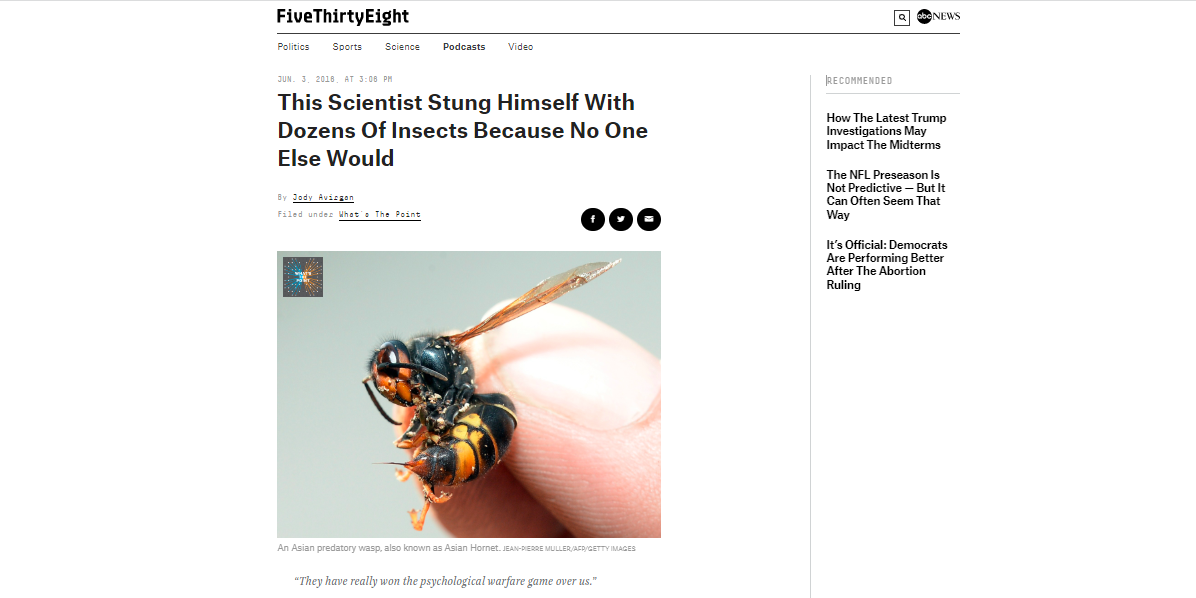
\includegraphics{png/inspiration/schmidt_pain_index.png}

}

\caption{Good data curators are people who share a passion for
measuring, recording and categorising the knowledge about their field,
be it insects, music, or informal economy.}

\end{figure}%

The \texttt{Schmidt\ Pain\ Index}, as its informally known, runs from
1-4. The common honey bee serves as its anchor point, a solid 2. At the
top end of the scale lie the bullet ant and the tarantula hawk (which is
neither a tarantula nor a hawk; it's
\href{https://www.wired.com/2015/07/absurd-creature-of-the-week-tarantula-hawk/}{a
wasp}). Watch the video with
\href{https://youtu.be/i0LjT-qkUes}{Dr.~Schmidt}, and listen to the
whole interview
\href{https://podcasts.apple.com/us/podcast/48-the-schmidt-sting-pain-index/id1011406983?i=1000391467968}{here}.
\href{https://fivethirtyeight.com/features/this-scientist-stung-himself-with-dozens-of-insects-because-no-one-else-would/}{⏯
This Scientist Stung Himself With Dozens Of Insects Because No One Else
Would}.

\subsection{Nobody Counted Them Before: Big Data Is Saving This Little
Bird}\label{nobody-counted-them-before-big-data-is-saving-this-little-bird}

``We need to improve conservation by improving wildlife monitoring.
Counting plants and animals is really tricky business.''
\href{https://fivethirtyeight.com/features/big-data-is-saving-this-little-bird/}{⏯
Big Data Is Saving This Little Bird}

\section{From Datasets and Files to Living Web
Resoures}\label{sec-web-30}

\subsection{Web 3.0}\label{web-3.0}

\begin{figure}[H]

{\centering 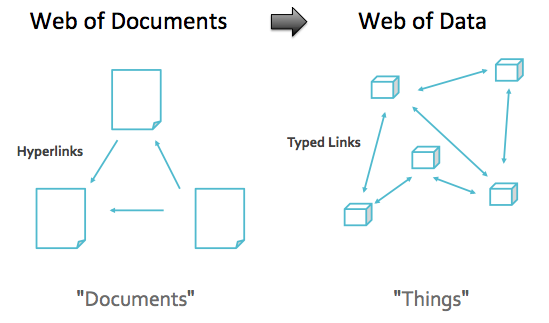
\includegraphics{png/inspiration/weblinks.png}

}

\caption{We are structuring your knowledge in a way that it results in
datasets that can be connected similarly to the World Wide Web pages.}

\end{figure}%

\section{Remain Critical: Ethical Data, Trustworthy
AI}\label{critical-attitude}

Sometimes we put our hands on data that looks like a unique starting
point to create a new indicator. But our indicator will be flawed if the
original dataset is flawed. And it can be flawed in many ways, most
likely that some important aspect of the information was omitted, or the
data is autoselected, for example, under-sampling women, people of
colour, or observations from small or less developed countries.

\subsection{Machine Learning from Bad Data: Weapons of Math Destruction,
Algorithms of
Oppression}\label{machine-learning-from-bad-data-weapons-of-math-destruction-algorithms-of-oppression}

Cathy O'Neil:
\href{https://en.wikipedia.org/wiki/Weapons_of_Math_Destruction}{⏯
Weapons of math destruction}, which O'Neil are mathematical models or
algorithms that claim to quantify important traits: teacher quality,
recidivism risk, creditworthiness but have harmful outcomes and often
reinforce inequality, keeping the poor poor and the rich rich. They have
three things in common: opacity, scale, and damage.
https://blogs.scientificamerican.com/roots-of-unity/review-weapons-of-math-destruction/{]}(https://blogs.scientificamerican.com/roots-of-unity/review-weapons-of-math-destruction/)

In \href{https://nyupress.org/9781479837243/algorithms-of-oppression/}{⏯
Algorithms of Oppression}, Safiya Umoja Noble challenges the idea that
search engines like Google offer an equal playing field for all forms of
ideas, identities, and activities. Data discrimination is a real social
problem; Noble argues that the combination of private interests in
promoting certain sites, along with the monopoly status of a relatively
small number of Internet search engines, leads to a biased set of search
algorithms that privilege whiteness and discriminate against people of
colour, especially women of colour.

\subsection{Big Data Creates Inequalities: Data
Feminism}\label{big-data-creates-inequalities-data-feminism}

Catherine D'Ignazio and Lauren F. Klein:
\href{https://mitpress.mit.edu/books/data-feminism}{⏯ Data Feminism}.
This is a much-celebrated book and with a good reason. It views AI and
data problems from a feminist point of view, but the examples and the
toolbox can be easily imagined for small-country biases, racial, ethnic,
or small enterprise problems. A very good introduction to the injustice
of big data and the fight for a fairer use of data, and how bad data
collection practices through garbage in-garbage out lead to misleading
information or even misinformation.

\subsection{Bad Data collection Used for Modeling: Why The Bronx
Burned}\label{bad-data-collection-used-for-modeling-why-the-bronx-burned}

\href{https://fivethirtyeight.com/features/why-the-bronx-really-burned/}{Why
The Bronx Burned}. Between 1970 and 1980, seven census tracts in the
Bronx lost more than 97 percent of their buildings to fire and
abandonment. In his book
\href{https://www.amazon.com/Fires-Computer-Intentions-City-Determined/dp/1594485062}{⏯
The Fires}, Joe Flood blames the misguided ``best and brightest'' effort
by New York City to increase government efficiency. With the help of the
Rand Corp., the city tried to measure fire response times, identify
redundancies in service, and close or re-allocate fire stations
accordingly. What resulted, though, was a perfect storm of bad data: The
methodology was flawed, the analysis was rife with biases, and the
results were interpreted in a way that stacked the deck against poorer
neighbourhoods. The slower response times allowed smaller fires to rage
uncontrolled in the city's most vulnerable communities. Listen to the
podcast
\href{https://podcasts.apple.com/us/podcast/19-why-the-bronx-burned/id1011406983?i=1000391467912}{here}.

\subsection{Bad Incentives Are Blocking Better
Science}\label{bad-incentives-are-blocking-better-science}

\href{https://fivethirtyeight.com/features/podcast-bad-incentives-are-blocking-better-science/}{Bad
Incentives Are Blocking Better Science} ``There's a difference between
an answer and a result. But all the incentives are pointing toward
telling you that as soon as you get a result, you stop.'' After the
deluge of retractions, the stories of fraudsters, the false positives,
and the high-profile failures to replicate landmark studies, some people
have begun to ask:
``\href{https://fivethirtyeight.com/features/science-isnt-broken/}{⏯ Is
science broken?}''. Listen to the pdocast {[}⏯Science is
Hard{]}tttps://podcasts.apple.com/us/podcast/10-science-is-hard/id1011406983?i=1000391467935)

\section{Reality Check}\label{reality-check}

\subsection{Looking Behind Data: Moving to America's Worst Place to
Live}\label{looking-behind-data-moving-to-americas-worst-place-to-live}

Christopher Ingraham wrote
\href{https://www.washingtonpost.com/gdpr-consent/?next_url=https\%3a\%2f\%2fwww.washingtonpost.com\%2fnews\%2fwonk\%2fwp\%2f2015\%2f08\%2f17\%2fevery-county-in-america-ranked-by-natural-beauty\%2f}{⏯
a quick blog post} for The Washington Post about an obscure USDA data
set called the \texttt{natural\ amenities\ index}, which attempts to
quantify the natural beauty of different parts of the country. He
described the rankings, noted the counties at the top and bottom, hit
publish and did not think much of it. Almost immediately, he started to
hear from the residents of northern Minnesota, who were not very happy
that Chris had written, ``The absolute worst place to live in America is
(drumroll, please) \ldots{} Red Lake County, Minn.'' He could not have
been more wrong \ldots{} a year later
\href{https://fivethirtyeight.com/features/he-called-it-americas-worst-place-to-live-now-hes-moving-there/}{he
moved} to Red Lake County with his family.

\bookmarksetup{startatroot}

\chapter{Tidy work}\label{sec-tidy}

\begin{quote}
Все счастливые семьи похожи друг на друга, каждая несчастливая семья
несчастлива по-своему. All happy families are alike; each unhappy family
is unhappy in its own way.
\end{quote}

Our \texttt{OpenCollections} systems are complex system which are
intended to be used in trustworthy AI applications. They follow the Anna
Karenina principle: a deficiency in any of a number of factors dooms an
endeavour to fail. Consequently, a successful endeavour (subject to this
principle) is one for which every possible deficiency has been avoided.

Once the data is messy, there is a semantic ambiguity (an ambiguity in
the intended use or meaning of data) that will render automation
impossible or will lead to logical faults when software agents or
algorithms use your data. You must keep your numeric and text data tidy
at all times. The best way to keep data and text tidy is to keep it
simple. Very simple.

Simplicity is simple, if you start simple and keep it that way.
Simplifying messy text and messy data is always challenging.

Collective work involving data and data annotations and descriptions
requires a shared understanding of the syntax and file formats.

Our curators need to be familiar with two ideas.

\begin{itemize}
\item[$\boxtimes$]
  Tidy data means that tabular datasets are organised in a simple but
  particular manner. All observations are in rows, and all measured
  variables or characteristics are in columns, with no merged columns or
  rows. This is the optimal formatting for working with relational
  databases, and it is also a helpful start for graph databases. (See:
  Section~\ref{sec-tidy-data}.)
\item[$\boxtimes$]
  Word processors like Word Work on different operational systems like
  Windows, MacOS, and Linux, creating very different text files and
  adding their formatting and other metadata to what you type. When we
  work together on the World Wide Web, we need something simpler than
  HTML but a bit more rich than a plain text file, clearly separating
  text editing from text formatting. The various markup notations, for
  example, \emph{markdown}, are conventions for indicating that you want
  to make a text part \textbf{bold} or \emph{italics} that works on all
  computer systems exactly the same way.(See:
  Section~\ref{sec-markup-text}.)
\end{itemize}

\section{Tidy data}\label{sec-tidy-data}

Our data stewardship must follow the tidy data principle, which has very
complex computer science and information management consequences, but
for the curators of data, it boils down to an organised simplicity.

Tidy data is a standard way of mapping the meaning of a dataset to its
structure. A dataset is messy or tidy depending on how rows, columns and
tables are matched up with observations or collection items, and the
measures and types of variables.

\begin{figure}[H]

{\centering \includegraphics{index_files/mediabag/tidy-1.png}

}

\caption{Following three rules makes a dataset tidy: variables are in
columns, observations are in rows, and values are in cells. From
\href{https://r4ds.had.co.nz/tidy-data.html}{R For Data Science - 12.
Tidy Data}}

\end{figure}%

In tidy data:

\begin{itemize}
\item[$\boxtimes$]
  \textbf{1. Every table column is a variable}. We do not use colours
  (our machine-to-machine pipelines is colourblind). If we need comments
  or specifications, we add a new column.
\item[$\boxtimes$]
  \textbf{2. Every row in the table represents an observation, or an
  individual piece of a collection.} Every variable belonging to
  \texttt{Bulgaria} is in the \texttt{Bulgaria} row, and there is one
  and only \texttt{Bulgaria\ row}.
\item[$\boxtimes$]
  \textbf{3. Every cell is a single value}. Your blue male apron length
  is 97? The length column of the blue male apron row is 97.
\end{itemize}

\begin{tcolorbox}[enhanced jigsaw, opacityback=0, bottomrule=.15mm, rightrule=.15mm, toptitle=1mm, breakable, colbacktitle=quarto-callout-note-color!10!white, colback=white, title=\textcolor{quarto-callout-note-color}{\faInfo}\hspace{0.5em}{Note}, leftrule=.75mm, toprule=.15mm, left=2mm, arc=.35mm, colframe=quarto-callout-note-color-frame, coltitle=black, titlerule=0mm, bottomtitle=1mm, opacitybacktitle=0.6]

A \texttt{tidy\ dataset} is black-and-white, and each table cells
contains one element of knowledge that cannot be further divided.

\end{tcolorbox}

We repeat in negative terms these seamingly simple principles:

\begin{itemize}
\item[$\square$]
  \textbf{Two observed values: two columns}. We do not use colours (our
  machine-to-machine pipelines is colourblind). If we need comments or
  specifications, we add a new column. The apron has a variable length
  of 96-98? Use a column for min and max length, and in the cases when
  there is a single number, put 97 as both max length and minimum
  length. But never write 96-98 in on column, it must be either 96 or
  98.
\item[$\square$]
  \textbf{Two items or two observations: two rows}: Do you have two
  types of blue male aprons: write a separate line for the kitchen apron
  and the gardening apron. Or just call it apron 1 and apron 2. Do you
  have two responsdents in the apron customer satisfaction form: that
  will be two rows.
\item[$\boxtimes$]
  \textbf{We never merge cells!} A tidy dataset has no divided or joined
  columns and no divided or joined rows. Never write 96-98 into a cell,
  because 96 goes to a separate cell than 98 because it has a different
  meaning: 96 means the minimum length of the apron, and 98 the maximum.
  Is there an apron with a length of 85 cm? That goes to a different
  row, because it refers to the length of a different type of apron.
\end{itemize}

Looks easy? If you start with a tidy table, it \emph{is} very easy. If
you have to tidy up a messy data table or an entire database, it often
requires many years of data-wrangling experience to get it right first.

Is there science behind this? Yes, and it is more complicated than it
sounds. In computer science or algebraic terms, you must organise your
data to Codd's 3rd standard form. If you start from a well-organised
table, it is a piece of cake to keep it that way. Reorganising messy
information into a tidy format requires a lot of experience.
Understanding that the ambiguity in the meaning of 96-98 should be
resolved by treating them as two separate values, one meaning minimum
possible length and the other maximum length, will not come naturally
for everybody. But we will help in those cases.

\subsection{Wide \& Long Formats}\label{wide-long-formats}

\begin{figure}[H]

{\centering 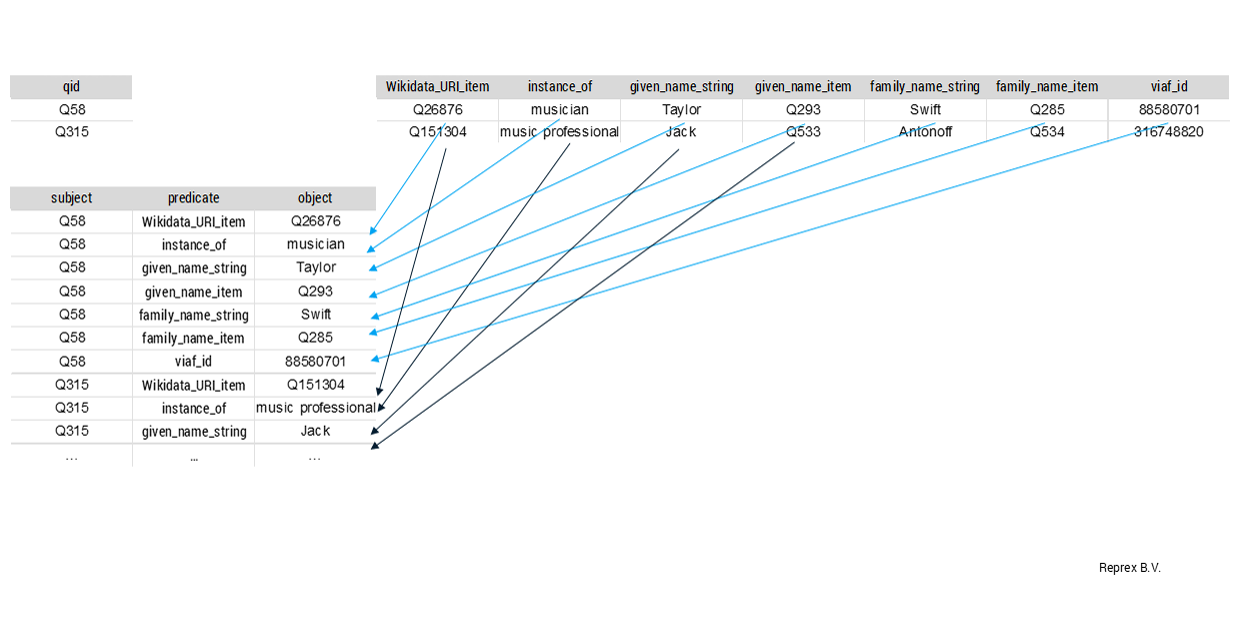
\includegraphics{png/tidy/pivot_longer_to_statements_notitle_2x1.png}

}

\caption{Tidy data tables can be pivoted: in this example a tidy
wide-format data table is pivoted to a long-form table which has exactly
three columns, a subject, a predicate and object, i.e., the semantic
triples of knowledge management.}

\end{figure}%

The tidy format is unambiguous: we always know that a number or string
(value) belongs to its observational subject (in the rows) and the
measured property variable (in the columns). Because the meaning is
unambiguous, it can be transposed to different formats without loss of
knowledge or misunderstandings.

Our knowledge base applications and Wikibase requires the three-column
semantic triple format, because it can be organised into a graph;
relational database managers usually prefer the wide format, because in
this case every observed property of a data subject is in one record.

\begin{tcolorbox}[enhanced jigsaw, opacityback=0, bottomrule=.15mm, rightrule=.15mm, toptitle=1mm, breakable, colbacktitle=quarto-callout-note-color!10!white, colback=white, title=\textcolor{quarto-callout-note-color}{\faInfo}\hspace{0.5em}{Note}, leftrule=.75mm, toprule=.15mm, left=2mm, arc=.35mm, colframe=quarto-callout-note-color-frame, coltitle=black, titlerule=0mm, bottomtitle=1mm, opacitybacktitle=0.6]

A \texttt{tidy\ dataset} is black-and-white, and each table cells
contains one element of knowledge that cannot be further divided.

\end{tcolorbox}

If your table is tidy, it will be easy to reuse in relational or graph
database, or it can import easily into a spreadsheet or statistical
program. Any further formatting with colours, divided columns, merged
rows will stop the data portability, because only you will know why
columns or rows are merged, divided, or coloured.

\section{Markup text}\label{sec-markup-text}

We create interconnected, interoperable (web) resources. We want to
ensure that our research results are findable, accessible, and reusable.
It must work in Word and Works, Notebook and VIM, Windows, MacOS, and
Linux, with Latvian, English, Greek, and Thai character sets.

The World Wide Web has been a source of high interoperability and
findability in the last 30 years, with the introduction of the HTTP
protocol and the standardization of the HTML text markup language. We
use a much-simplified version of HTML called Markdown.

Markdown text opens on MacOS, Windows, or Linux. It is very easy to
translate into HTML, Word, Libre Office, Google Docs, LaTeX, or PDF.
Markdown is a simplified HTML text notation that works well with word
processors.

\begin{center}
\includegraphics{index_files/mediabag/markdown-flowchart.png}
\end{center}

If you want Word output, Word is rendered instead of HTML. You can also
create a PDF or EPUB and even a PPTX output.

\subsection{Markdown editors}\label{markdown-editors}

There are countless Markdown editors. Because Markdown is so simple, you
can, if you want to, edit markdown files in Notepad, WordPad (Windows)
or VIM (Linux).

Most word processors support markdown. For example, Google Docs has a
\href{https://workspace.google.com/marketplace/app/docs_to_markdown/700168918607}{free
extension} that converts and document from Docs to markdown.

\begin{figure}[H]

{\centering 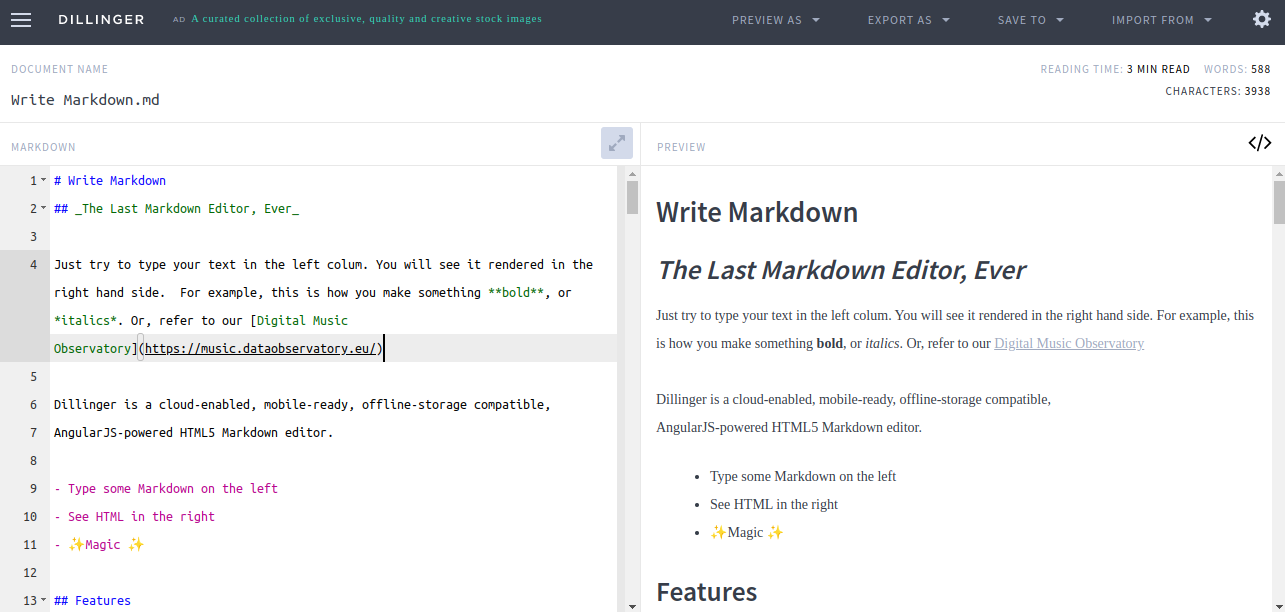
\includegraphics{png/dilliger_example.png}

}

\caption{Dilinger is one of the best editors, and it is particularly
suitable foor first-time markup users, as you immediately get visual
feedback on how you mark up your text.}

\end{figure}%

There are several online Markdown editors that you can use to try
writing in Markdown. \href{https://dillinger.io/}{Dillinger} is one of
the best online Markdown editors. Just open the site and start typing in
the left pane. A preview of the rendered document appears in the right
pane.

\begin{itemize}
\tightlist
\item
  \href{https://www.markdownguide.org/basic-syntax/}{Basic Syntax}
\item
  \href{https://www.markdownguide.org/extended-syntax/}{Extended Syntax}
\end{itemize}

\begin{tcolorbox}[enhanced jigsaw, opacityback=0, bottomrule=.15mm, rightrule=.15mm, toptitle=1mm, breakable, colbacktitle=quarto-callout-tip-color!10!white, colback=white, title=\textcolor{quarto-callout-tip-color}{\faLightbulb}\hspace{0.5em}{Using Word or Works}, leftrule=.75mm, toprule=.15mm, left=2mm, arc=.35mm, colframe=quarto-callout-tip-color-frame, coltitle=black, titlerule=0mm, bottomtitle=1mm, opacitybacktitle=0.6]

You can work on Word, your iWorks suite, or any preferred word
processor. However, you will lose margin settings, font typefaces and
sizes, background colors, and other finishing touches.

We discourage the use of word processors for footnotes and bibliographic
references due to their varying treatment of such metadata. Our systems
rely on standard BibLatex bibliographic references and a simple notation
for footnotes, ensuring consistency and reliability.

Our recommended markdown editor is Quarto. You can copy and paste text
from Word or other word processors into Quarto, and it will retain
\textbf{bold}, \emph{italics}, and headings.

Remember, we want to create text that machines and people can read, too,
to avoid fancy aesthetics. Keep the text fancy (but of course, you can
dress it up in Word or Adobe Illustrator later).

\end{tcolorbox}

\subsection{Wikipedia \& MediaWiki}\label{wikipedia-mediawiki}

The documentation of our knowledge base and terminological agreements is
documented in MediaWiki, the software that makes Wikipedia editable,
too. It uses a form of markdown for an interoperable and simple editing
of interlinked documents, images, and data documents.

\bookmarksetup{startatroot}

\chapter{Collections}\label{sec-collections}

The term ``collection'' is elusive. Museums, libraries, and archives
have never reached a consensus on what it means because there are so
many ways and motivations to collect things. Physical collections often
spoke for themselves. The idea of a digital collection made the process
of collecting more abstract and fuzzy, as we can generate very large and
heterogeneous collections.

Our manual aims to remain practical and seeks no definition of
collection or curation. For our purposes, a digital collection is an
organised set of digital artefacts organised by a curator or successive
curators in institutions, following a more or less well-defined policy.
The collection aims to preserve digital artefacts that users can use or
consult, and the users need to find these artefacts: books, articles,
photographs, historical dresses, sound recordings, stamps, and
biographies. To retrieve individual items from the collection, we employ
names (name titles) and identifiers, and to help with searching,
browsing, and learning, we use categorisations in the collection.

\section{Curator}\label{curator}

Curators of physical collections have been recognised as professionals
who search, acquire, preserve, research and communicate the individual
items of collections to be preserved for further generation in musea:
``\ldots the notions of curation and curator to denote the person in
charge of all tasks directly related to objects in a museum collection
(i.e.~their preservation, research, and communication) become firmly
established in the English-speaking world only as late as the nineteenth
century, their generalised use coinciding with the rise of museum
professionalism.'' (Dallas 2016)

In the digital era, without the limitations of transport costs, storage
space costs, temperature or lightning requirements, we can create much
larger collections; on the Internet they can attract a global user base.
Digital curation requires a reflection on the physical curatorial
policies.

\begin{quote}
``In a pragmatic approach, actors of digital curation include not just
information professionals but also those involved in all aspects of the
creation and reuse of a broad range of information objects. The latter
comprise not just digital research data, static digital resources, and
databases, but also derivations and performances of such objects, and
representations of domain knowledge, including indigenous and community
based.'' (Dallas 2016)
\end{quote}

\section{Collection types}\label{collection-types}

\subsection{Playlists, repertoires,
libraries}\label{playlists-repertoires-libraries}

The archetype of libraries contains books organized by title, author and
topic, or music libraries by title, author and genre.

Library-type collections use the Dublin Core metadata set, organized
around titles, authors, and short descriptions.

\begin{tcolorbox}[enhanced jigsaw, opacityback=0, bottomrule=.15mm, rightrule=.15mm, toptitle=1mm, breakable, colbacktitle=quarto-callout-tip-color!10!white, colback=white, title=\textcolor{quarto-callout-tip-color}{\faLightbulb}\hspace{0.5em}{Libraries, playlist}, leftrule=.75mm, toprule=.15mm, left=2mm, arc=.35mm, colframe=quarto-callout-tip-color-frame, coltitle=black, titlerule=0mm, bottomtitle=1mm, opacitybacktitle=0.6]

Your collection will likely depend on the Dublin Core, DataCite or
Europena mandatory metadata fields. For example, to place an item of
your collection into Europeana you must identify each item with a
\texttt{title} and/or a \texttt{description}; in a library system you
will use titles, often with subtitles or alternative (translated)
titles.

\begin{itemize}
\tightlist
\item[$\boxtimes$]
  You will use the names of author(s), like \emph{Mark Twain}, or
  \emph{John Lennon} and \emph{Paul McCartney}.
\item[$\boxtimes$]
  You will use titles, like \emph{The Adventures of Huckleberry Finn}
  and \emph{Hey Jude} and \emph{Symphony No.~2.}. Literary works and
  classical music works often have translated titles like \emph{2.
  szimfónia}.
\item[$\boxtimes$]
  You will use publication or public release or copyright registration
  dates (or at least years.)
\end{itemize}

Because there may be several identically named authors or titles (think
about the Symphony No.~2.), you will need unique identifiers for your
items.

\end{tcolorbox}

Libraries suffer from name ambiguities and often name entity
disambiguation. For example, many songs are called ``Machinist,'' and
many authors are called ``James Campbell.'' Sometimes, names and titles
need to be matched, which causes search errors, royalty payment errors,
etc. See further details in the subsequent
Section~\ref{sec-naming-individual-entities} part of this chapter.

\subsection{Webshops, galleries,
museums}\label{webshops-galleries-museums}

Galleries and other exhibition places often show only (on the front
page) a selection of diverse items available in your inventory. You do
not only keep books or sound recordings but also keep various items
(merchandise, tote bags, etc.); the items need to be better described
with author-title relationships; after all, who is the `author' of a
tote bag?

Gallery-type collections use a CIDOC-like information model for metadata
and usually rely more heavily on thesauri to describe many different
entities or things with a consistent language that is well understood by
machines and people alike.

\begin{tcolorbox}[enhanced jigsaw, opacityback=0, bottomrule=.15mm, rightrule=.15mm, toptitle=1mm, breakable, colbacktitle=quarto-callout-tip-color!10!white, colback=white, title=\textcolor{quarto-callout-tip-color}{\faLightbulb}\hspace{0.5em}{Webshops, galleries, museums}, leftrule=.75mm, toprule=.15mm, left=2mm, arc=.35mm, colframe=quarto-callout-tip-color-frame, coltitle=black, titlerule=0mm, bottomtitle=1mm, opacitybacktitle=0.6]

Your collection will likely depend on a broader conceptual model like
CIDOC, and well-established controlled vocabularies like AAT.

\begin{itemize}
\item[$\boxtimes$]
  You will use titles, like \emph{Mona Lisa} and \emph{Ohne Titel}.
  Titles are often translated (\emph{Without title}) or not useful for
  identification (like \emph{Ohne Titel}).
\item[$\boxtimes$]
  Because the title may not be a good identifier, you will use short
  descriptions, like Tour \emph{T-Shirt Female Medium}, \emph{Tour
  T-Shirt Male XL}, \emph{Blue kitchen apron from the 19th century}. In
  such cases, the title may be a shorter version of the description
  \emph{This wonderful Tour T-Shirt is available in blue, yellow, and
  green for women}.
\item[$\boxtimes$]
  Various further information points on provenance may be recorded
  (``Designed in California'', ``Found in the Friesland region of the
  Netherlands'') etc.
\end{itemize}

Good descriptions are essential because your users may look for very
different items in your collections. Good descriptions can be easily
translated from English to Dutch or Latvian, and machines can read them
or translate them without error. You will focus on using keywords,
keyword chains, or descriptions that come from a controlled vocabulary,
a classification, or a thesaurus.

Unless your enterprise or organisation has its ontology, we will use
CIDOC as a basis. CIDOC is a complex, event-based information model and
you do not have to learn it. We need to ensure that the most important
metadata about your collection is imported or entered into Wikibase so
that we can export it, for example, into a CIDOC-compliant RDF.

\end{tcolorbox}

The challenge with galleries is that they have to describe many things
consistently and independently from natural languages. For example, a
dress historian may use the colour
\href{http://vocab.getty.edu/page/aat/300129361}{blue} to describe a
\href{http://vocab.getty.edu/page/aat/300422315}{cooking aprons}. How do
we make sure that \texttt{blue}, \texttt{blauw}, \texttt{kék},
\texttt{ლურჯი}, or \texttt{синий}, labels are understood the same way,
so that we can compare English, Dutch, Russian or Georgian collections?
(See Section~\ref{sec-nerd} later in this chapter.)

\subsection{Documents, question banks,
archives}\label{documents-question-banks-archives}

Archives and document databases often contain millions of various
documents or other records. Compared to libraries and galleries,
individual collection items usually have a lower value and a much lower
level of documentation. An archive may contain millions of documents,
but only a few may be interesting for our age or use case. Titles are
often non-existent because the \texttt{document\ \#3217454} is not very
helpful for the user.

Archives emphasize the provenance of their collections. We may have
thousands of emails, which must be those of a late novelist or a former
CEO. If they are boxed, the origin of the box, when it was boxed, and
other aspects of their recording history are the most important guides
for the person who wants to find \emph{that} email sent to the editor
about the final changes in a novel, or the \emph{final aproval} of an
investment project.

Archives use the RiC conceptual model, ontology, or a metadata system on
prior international archival standards.

\subsection{Registers}\label{sec-collections-registers}

Registers are collections that aim for completeness. They register every
limited liability company in a jurisdiction, every copyright-protected
musical work in a country, every living person, and every living
musician in a city.

Registers can be library-like (for example, for copyright-protected
literary or musical works), or more archival, for registering every
birth and death certificate to create a population register. Like in the
case of archives, data provenance is important. As opposed to archives,
registers add new items and delete or make them obsolete; when people
move away, companies are liquidated, or the copyright term of musical
work expires.

\begin{tcolorbox}[enhanced jigsaw, opacityback=0, bottomrule=.15mm, rightrule=.15mm, toptitle=1mm, breakable, colbacktitle=quarto-callout-tip-color!10!white, colback=white, title=\textcolor{quarto-callout-tip-color}{\faLightbulb}\hspace{0.5em}{From business records to archives}, leftrule=.75mm, toprule=.15mm, left=2mm, arc=.35mm, colframe=quarto-callout-tip-color-frame, coltitle=black, titlerule=0mm, bottomtitle=1mm, opacitybacktitle=0.6]

Your main challenge is that you have many very similar items in your
collections, which are usually not very interesting and therefore
researchers or curators do not spend time to individual describe and
title them.

\begin{itemize}
\tightlist
\item[$\boxtimes$]
  It is important to retain information about the record's structure:
  the letter has 3 pages, and the individual page is the 2nd of 3 pages.
\item[$\boxtimes$]
  Provenance is recorded with utmost care: the letters from the private
  drawer of the CEO, the private journal of the author, and the
  company's the counts in the year 1832.
\item[$\boxtimes$]
  Like libraries, our role is to connect people to the collection item,
  broadening the understanding of its significance. This connection is
  not limited to an author or editor role but extends to various roles
  such as project sponsor, judge, correspondence partner, sibling, etc.
\end{itemize}

The international archival standards were modernised into RiC (Records
in Context) for linking on the internet in 2023. We use the RIC ontology
and conceptual model to work with archival documents. Our curators do
not have to work with RIC directly in all cases, but they must use
OpenCollections in a way that records they record the key metadata of
RIC. We will set up a Wikibase for you in a way that can be translated
to RIC (and earlier archival standards.)

\end{tcolorbox}

Registers can be formed around libraries, galleries, and archives, but
they always have a time dimension, showing valid from and valid till
date of every item.

\section{Identifying, Naming, and Describing Collection
Items}\label{identifying-naming-and-describing-collection-items}

\subsection{Naming people and indvidual
things}\label{sec-naming-individual-entities}

When interacting with the world of persons, things, and relations, we
use human language and name the persons and things. When naming people,
for example, we use a first name or a full name. Names can be
unambiguous or have a certain level of ambiguity that can be resolved in
a context. In the United States alone, more than 38,000 men were named
James Smith, and more than 32,000 women were named Maria Garcia in 2013
(Hartman n.d.); identification by full name is an error-prone process.

\texttt{Taylor} is a unisex English name, and \texttt{Swift} is a family
name that is not uncommon in English-speaking countries. The full name
\texttt{Taylor\ Swift} name can refer to the American female superstar
Taylor (Alison) Swift, the American male photographer Taylor Swift, or
the event manager of Grand Hyatt New York, a woman who grew up in
Missouri and used to sing in groups. (Newsweek:
\href{https://www.newsweek.com/two-people-named-taylor-swift-talk-about-being-named-taylor-swift-age-taylor-283861}{What
It's Like to Be Named Taylor Swift in 2014})

Taylor M. Swift, woman from New York:

\begin{quote}
Taylor Swift, New York: Facebook shut off my profile because they
thought I was impersonating her. She must have been 15, so I was 18 or
19. She started to get popular and Facebook contacted me saying, ``We
are so sorry, but any impersonation of any kind is forbidden.'' I sing,
too, and in college I was in a singing group and they thought I was
literally impersonating her because people would write on my wall
{[}about performances{]}. I had to send in three forms of ID. I think it
took three-and-a-half weeks to get it back. Now my {[}Facebook{]} name
is Taylor {[}middle name{]} because I can't have my first and last name
on there\ldots{} On my business cards, I have Taylor M. Swift.
\end{quote}

Another Taylor Swift, a man from Seattle:

\begin{quote}
Taylor Swift, Seattle: I get probably two or three emails {[}meant for
Swift{]} a day. I've incorporated my middle name into my primary email,
but I've held onto that one because why not?
\end{quote}

The management of large collections and their databases requires
unambiguous identification. It is avoidable that Taylor Swift, the
photographer in Seattle, receives the royalties of the
\texttt{Gold\ Rush} song; it is equally unacceptable that he cannot sell
his photographs because his name is confused with the famous musician's
namesake.

The names are replaced with a unique string in a database or an
application that works with databases, like a museum inventory book, a
copyright register, or a library catalogue. This string is often a
string of numeric digits.

\begin{itemize}
\item
  \texttt{Uniqueness}: a given identifier must specify (``point to'')
  one and only one person in the name space; in a personal record
  collection, there may not be identically named artist, however, in a
  global collection like the complete catalogue of Spotify, YouTube or
  Apple Music, there are many namesakes. With the ability to connect,
  link, join digital collections, names are less and less likely to be
  unique.
\item
  \texttt{Persistence}: people's names are not permanent, and do not
  enable unambiguous specification of entities for an indefinite period.
  In many cultures, people change names when married (or divorced),
  particularly women; but there are many other reasons for a change of a
  person's name. In music and other arts, artist often use pseudonyms
  from a given time period.
\end{itemize}

\begin{tcolorbox}[enhanced jigsaw, opacityback=0, bottomrule=.15mm, rightrule=.15mm, toptitle=1mm, breakable, colbacktitle=quarto-callout-tip-color!10!white, colback=white, title=\textcolor{quarto-callout-tip-color}{\faLightbulb}\hspace{0.5em}{Tips for people's names}, leftrule=.75mm, toprule=.15mm, left=2mm, arc=.35mm, colframe=quarto-callout-tip-color-frame, coltitle=black, titlerule=0mm, bottomtitle=1mm, opacitybacktitle=0.6]

\begin{itemize}
\tightlist
\item[$\boxtimes$]
  Try to record all name variants.
\item[$\boxtimes$]
  Be aware of the differences of the Eastern and Western name order.
\item[$\boxtimes$]
  Thrive to use global, unique, persistent identifiers.
\item[$\boxtimes$]
  When there is no truly global identifier, create one in
  OpenCollections.
\end{itemize}

\end{tcolorbox}

The \texttt{Eiffel\ Tower}, \texttt{Tour\ Eiffel},
\texttt{Eiffel-torony}, \texttt{Eiffeltoren} names refer to the same
building in English, French, Hungarian and Dutch. While the building is
individual, it has many names. Using a street address or the
geocoordinates would be tempting; but street addresses keep changing.
The geocoordinates do not show elevation (in case you would need the
storey number), and there was \emph{something} in another time, before
the Eiffel Tower was built on the location of 48° 51' 29.1348'\,' North
and 2° 17' 40.8984'\,' East. A popular location identifier,
\texttt{geonames} identifies this famous building with
\href{https://www.geonames.org/6254976/tour-eiffel.html}{6254976};
Wikidata uses the \href{https://www.wikidata.org/wiki/Q243}{Q243}
identifier.

The \texttt{Symphony\ No.\ 2} suffers from the same problem (it is
\texttt{2.\ szimfónia} in Hungarian and \texttt{Symfonie\ nr.\ 2} in
Dutch), but also from the fact that it is given to many musical works:
it may refer to Opus 36 of Ludwig van Beethoven
(\href{https://www.wikidata.org/wiki/Q210451}{Symphony No.~2 in D Major,
Op. 36}), or \href{https://www.wikidata.org/wiki/Q210549}{Symphony No.~2
in C Minor} by Gustav Mahler, or
\href{https://www.wikidata.org/wiki/Q210469}{Opus 73, Symphony No.~2 in
D Major}, by Johannes Brahms.

In collections, ``information for display should be in a format and with
syntax that is easily read and understood by users. This may be
accomplished through data in the form of free text or concatenated
displays, allowing for the expression of the nuances of language
necessary to relay the uncertainty and ambiguity that are common in art
information.'' (Harpring and Baca 2016, p429) Most collection management
systems use a \texttt{title} and a \texttt{description} field to achieve
this effect; titles and descriptions are used in library, archive and
museum-type memory institutions. Software codes and information systems
also need good names, and coming up with good names is often considered
as the one of the most difficult task in computer science. (Allamanis et
al. 2015)

\begin{tcolorbox}[enhanced jigsaw, opacityback=0, bottomrule=.15mm, rightrule=.15mm, toptitle=1mm, breakable, colbacktitle=quarto-callout-tip-color!10!white, colback=white, title=\textcolor{quarto-callout-tip-color}{\faLightbulb}\hspace{0.5em}{Tips for individual names of things}, leftrule=.75mm, toprule=.15mm, left=2mm, arc=.35mm, colframe=quarto-callout-tip-color-frame, coltitle=black, titlerule=0mm, bottomtitle=1mm, opacitybacktitle=0.6]

\begin{itemize}
\tightlist
\item[$\boxtimes$]
  Choose a preferred name that is easy to read, and may be understood
  for most (or a plurality) of your users.
\item[$\square$]
  It may not be possible to record all name variants; use the ones that
  may be relevant for your users.
\item[$\boxtimes$]
  Thrive to use global, unique, persistent identifiers.
\item[$\boxtimes$]
  When there is no truly global identifier, create one in
  OpenCollections.
\end{itemize}

\end{tcolorbox}

\subsection{Naming categories, groups of individual entities, and
non-individual
items}\label{naming-categories-groups-of-individual-entities-and-non-individual-items}

\begin{quote}
When discussing art vocabulary for categorizing works of art, we are
really talking about the controlled terminology used to \emph{index} art
works. For our purposes, \emph{indexing} refers to a conscious activity
performed by knowledgeable cataloguers who consider the retrieval
implications of the indexing terms that they apply to information
objects; we are not referring to an automated process that simply parses
every word in a text into indexes, as search engines like Google do on
the open Web. Controlled vocabulary for art refers to standardised words
and phrases used to refer to ideas, physical characteristics, people,
places, events, subject matter, and many other concepts related to art,
architecture, and other cultural heritage. The most important functions
of a controlled vocabulary are to gather together variant terms and
synonyms referring to concepts, and to link concepts in a logical order
or into categories. Are a \emph{rose window} and a \emph{Catherine
wheel} the same thing? How is \emph{pot-metal glass} related to the more
general term \emph{stained glass}? The links and relationships in a
controlled vocabulary ensure that these relationships are defined and
maintained, for both cataloguing and retrieval.(Harpring and Baca 2016,
p426)
\end{quote}

Information for display should be in a format and with syntax that is
easily read and understood by users. This may be accomplished through
data in the form of free text or concatenated displays, allowing for the
expression of the nuances of language necessary to relay the uncertainty
and ambiguity that are common in art information. In addition, certain
key elements of information must be formatted to allow for retrieval,
using controlled vocabularies where appropriate.

\begin{tcolorbox}[enhanced jigsaw, opacityback=0, bottomrule=.15mm, rightrule=.15mm, toptitle=1mm, breakable, colbacktitle=quarto-callout-tip-color!10!white, colback=white, title=\textcolor{quarto-callout-tip-color}{\faLightbulb}\hspace{0.5em}{Tips for naming things}, leftrule=.75mm, toprule=.15mm, left=2mm, arc=.35mm, colframe=quarto-callout-tip-color-frame, coltitle=black, titlerule=0mm, bottomtitle=1mm, opacitybacktitle=0.6]

\begin{itemize}
\tightlist
\item[$\boxtimes$]
  Whenever possible, use an open, public, trusted controlled vocabulary
  or thesaurus to create generic names (``male shirt'')
\item[$\square$]
  It is a good practice to use several thesauri, even though for
  usability a preferred (main) thesaurus may be preferred.
\item[$\boxtimes$]
  Use the same controlled vocabularies to identify categories,
  subgroups, keywords.
\item[$\boxtimes$]
  Thrive to use global, unique, persistent identifiers of the
  definitions of your controlled vocabulary.
\item[$\boxtimes$]
  When there is no truly global definition, create one in
  OpenCollections.
\end{itemize}

\end{tcolorbox}

\section{Identifiers}\label{identifiers}

``An identifier is an unambiguous label which specifies an entity. In
computer science terms, an identifier is a name; the entities named
occupy a specific domain of application,the namespace, and identify
points in that namespace.'' (N. Paskin 1999)

\begin{itemize}
\item
  \texttt{Uniqueness}: a given identifier must specify (``point to'')
  one and only one person or thing in the name space. If we work on the
  internet, then the identifier must be a globally unique string,
  because the name space can perpetually grow.
\item
  \texttt{Persistence}: is permanence of naming, enabling unambiguous
  specification of entities for an indefinite period.
\end{itemize}

\begin{quote}
A numbering scheme is a formal standard, an industry convention, or an
arbitrary internal system such as an incremented production serial
number etc., to arrive at a consistent syntax for denoting and
distinguishing separate members of a class of entities. {[}\ldots{]} The
important point here is that the resulting number is simply a label
string (a ``noun''). It does not, of itself, create a string that is
actionable in a digital or physical environment (a ``verb'') without
further steps being taken. It may be used (and probably will be used) in
databases, or it may be incorporated into another mechanism later.
(Norman Paskin 2003, 30--31).
\end{quote}

Because modern IT systems can contain information about billions and
billions of things, it is less and less desirable to only use the
0\ldots9 numeric characters for this purpose, and often, a random string
of alphanumeric characters is used. Many so-called hash applications
ensure that even if you record billions of entities or transactions,
they are given a unique string. Following Norman Paskin, it is a good
distinction to consider these identifiers as a simple label string or a
``noun''. \texttt{0000\ 0004\ 6613\ 4394} is simply a computer-language
equivalent of Taylor (Alison) Swift; it is the International Standard
Name Identifier for the said artist. In the universe of the Spotify
music platform, the string
\href{https://open.spotify.com/artist/06HL4z0CvFAxyc27GXpf02}{06HL4z0CvFAxyc27GXpf02}
identifies the same famous artist.

\begin{itemize}
\item[$\boxtimes$]
  A library catalogue contains information about books. Books are
  usually identified by title, author name, publisher, and publishing
  data because often the same library has many James Campbells or
  similar-titled books, etc. A unique global identifier is the
  International Standard Book Number.
\item[$\boxtimes$]
  A music playlist contains sound recordings. The recordings are often
  referred to by the name of the performer(s) and the title of the music
  work that they perform; however, in global systems, we may have dozens
  of same-name performers and even hundreds of same-title works (just
  think about Symphony No.2!). Instead, we can identify the performers
  with the ISNI International Standard Name Identifier and the
  recordings with the Spotify Track ID or the ISRC International
  Standard Recording Code.
\item[$\boxtimes$]
  A dress history database may identify specimens of shirts and aprons;
  as there may be many similar aprons, they usually do not have a
  specific name. Instead, they are either identified with a generic
  name, like \texttt{Male\ apron\ from\ the\ 19th\ century}, or by an
  inventory number.
\end{itemize}

\begin{tcolorbox}[enhanced jigsaw, opacityback=0, bottomrule=.15mm, rightrule=.15mm, toptitle=1mm, breakable, colbacktitle=quarto-callout-note-color!10!white, colback=white, title=\textcolor{quarto-callout-note-color}{\faInfo}\hspace{0.5em}{Note}, leftrule=.75mm, toprule=.15mm, left=2mm, arc=.35mm, colframe=quarto-callout-note-color-frame, coltitle=black, titlerule=0mm, bottomtitle=1mm, opacitybacktitle=0.6]

The most common standard numbering schemes of interest in digital rights
management and digital asset management include

\begin{itemize}
\tightlist
\item
  ISBN: International Standard Book Numbering (ISBN)
\item
  ISSN: International Standard Serial Number (ISSN)
\item
  ISRC: International Standard Recording Code (ISRC)
\item
  ISRN: International Standard Technical Report Number (ISRN)
\item
  ISMN: ISO 10957:1993 International Standard Music Number (ISMN)
\item
  ISWC: ISO 15707:2001 International Standard Musical Work Code (ISWC)
\item
  ISAN: Draft ISO 15706: International Standard Audiovisual Number
  (ISAN)
\item
  ISTC: Draft ISO 21047: International Standard Text Code (ISTC)
\end{itemize}

\end{tcolorbox}

\subsection{Actionable identifiers}\label{actionable-identifiers}

Paskin calls identifiers that can initiate an action in a digital or
physical environment actionable identifiers, similar to verbs.

If in your home database, \texttt{artist-0001} refers to Taylor Swift,
it is just a ``noun'', a replacement of Taylor Swift. However,
\href{https://isni.org/isni/0000000078519858}{0000 0004 6613 4394} and
\href{https://open.spotify.com/artist/06HL4z0CvFAxyc27GXpf02}{06HL4z0CvFAxyc27GXpf02}
are actionable. Clicking \url{https://isni.org/isni/0000000078519858}
informs you via your browser or your library system by sending a package
of standard metadata that this woman is not Taylor M. Swift from New
York or the Taylor Swift, the photographer from Seattle. Similarly,
\url{https://open.spotify.com/artist/06HL4z0CvFAxyc27GXpf02} allows you
to check out and even listen to all the released songs of the most
famous Taylor Swift.

\subsection{Local and global
identifiers}\label{local-and-global-identifiers}

\texttt{Τέιλορ\ Σουίφτ}, \texttt{ტეილორ\ სვიფტი} both stand for ``Taylor
Swift'' with different character sets and \texttt{Teilora\ Svifta} is a
Latvian version of the same name. We can say that they are suitable in a
Greek, Georgian or Latvian database. Similarly, database management
systems provide (local) unique identifiers for every CD or music sheet
of the author.

If in your home database, \texttt{artist-0001} may refer to the same
artist. The problem with connecting databases and exchanging information
about the the artist known as ``Taylor Swift'' is to ensure that
\texttt{artist-0001}, \texttt{Teilora\ Svifta} is exchanged with data
about \href{https://isni.org/isni/0000000078519858}{0000 0004 6613
4394}, or
\href{https://open.spotify.com/artist/06HL4z0CvFAxyc27GXpf02}{06HL4z0CvFAxyc27GXpf02},
or \texttt{ტეილორ\ სვიფტი,} and not the photographer Taylor Swift or any
other person.

\texttt{Taylor\ Swift} is a name, not an identifier. In most contexts,
it correctly identifies Taylor M. Swift, Taylor Swift, and Taylor Alison
Swift, but there are mistakes.

\begin{itemize}
\item
  \href{https://open.spotify.com/artist/06HL4z0CvFAxyc27GXpf02}{06HL4z0CvFAxyc27GXpf02}
  is a local but public identifier. It works only in the Spotify
  universe, but you can check that any music connected to
  \texttt{06HL4z0CvFAxyc27GXpf02} is performed by Taylor Swift.
\item
  \href{https://isni.org/isni/0000000078519858}{0000000078519858} is a
  global identifier because the ISNI consortium ensures that nobody will
  ever get the same identifier again; furthermore, the identifier
  follows an international standard and remains forever open.
\end{itemize}

Global identifiers aim to work across databases; they are not specific
to your computer system or a specific library catalogue. The use of
global identifiers is essential to making various databases, data
carriers, or their systems interoperable.

The line between
\href{https://open.spotify.com/artist/06HL4z0CvFAxyc27GXpf02}{06HL4z0CvFAxyc27GXpf02}
and \href{https://isni.org/isni/0000000078519858}{0000000078519858} is
blurred. Both can be used almost all over the world, and the basic
services of
\href{https://open.spotify.com/artist/06HL4z0CvFAxyc27GXpf02}{06HL4z0CvFAxyc27GXpf02}
are free. Spotify offers plenty of relevant music metadata and
statements for free via its web player and its open API about Taylor
Swift.

\section{Identifiers and metadata}\label{identifiers-and-metadata}

\begin{quote}
The most common---and perhaps least useful---definition of metadata is
that it is ``data about data.'' As catchy as this definition is,
however, it is entirely ambiguous. First of all, what is data? And
second, what does ``about'' mean? (Pomerantz 2015, p19)
\end{quote}

We use the definition of Pomerantz about metadata. The new ISO standard
on Information technology --- Metadata registries (MDR) defines
\emph{metadata} as data that defines and describes other data. As
Pomerantz eloquently argues, this definition is not very helpful. We use
his more functional (but not contradictory) definition. ``Data is only
potential information, raw and unprocessed, prior to anyone actually
being informed by it. {[}\ldots{]} Data must be understood not as an
abstract concept but as objects that are potentially informative.
{[}\ldots{]} Metadata Is a Statement about a Potentially Informative
Object.'' (Pomerantz 2015, p26)

A \texttt{statement} in this semantic meaning is a meaningful
declarative sentence that is either true or false.

\begin{itemize}
\tightlist
\item
  Taylor Swift was born in 1989.
\end{itemize}

The World Wide Web standards for metadata exchange, which are
quasi-global standards, work with so-called semantic triples. Triples
are the shortest possible statements: they connect a subject and an
object through a predicate.

The most popular metadata language that is both human- and
machine-readable, Turtle ends every statement with a dot space separated
from the third element of a triple (to avoid the third string having a
dot character).

\begin{Shaded}
\begin{Highlighting}[]
\CommentTok{\# The URLs for the definitions:}
\SpecialCharTok{@}\NormalTok{prefix person}\SpecialCharTok{:} \ErrorTok{\textless{}}\NormalTok{http}\SpecialCharTok{:}\ErrorTok{//}\NormalTok{example.org}\SpecialCharTok{/}\NormalTok{persons}\SpecialCharTok{/}\ErrorTok{\textgreater{}}
\ErrorTok{@}\NormalTok{prefix relation}\SpecialCharTok{:} \ErrorTok{\textless{}}\NormalTok{http}\SpecialCharTok{:}\ErrorTok{//}\NormalTok{example.org}\SpecialCharTok{/}\NormalTok{relations}\SpecialCharTok{/}\ErrorTok{\textgreater{}}
\ErrorTok{@}\NormalTok{prefix book}\SpecialCharTok{:} \ErrorTok{\textless{}}\NormalTok{http}\SpecialCharTok{:}\ErrorTok{//}\NormalTok{example.org}\SpecialCharTok{/}\NormalTok{books}\SpecialCharTok{/}\ErrorTok{\textgreater{}}
\ErrorTok{@}\NormalTok{prefix works}\SpecialCharTok{:} \ErrorTok{\textless{}}\NormalTok{http}\SpecialCharTok{:}\ErrorTok{//}\NormalTok{example.org}\SpecialCharTok{/}\NormalTok{musical\_works}\SpecialCharTok{/}\ErrorTok{\textgreater{}}
  
\CommentTok{\# Simple triple statements:}
  
\NormalTok{person}\SpecialCharTok{:}\NormalTok{Mark\_Twain   relation}\SpecialCharTok{:}\NormalTok{author books}\SpecialCharTok{:}\NormalTok{Huckleberry\_Finn .}
\NormalTok{person}\SpecialCharTok{:}\NormalTok{Taylor\_Swift relation}\SpecialCharTok{:}\NormalTok{author works}\SpecialCharTok{:}\NormalTok{Gold\_Rush .}
\end{Highlighting}
\end{Shaded}

The standard \emph{Japanese breakfast} consists of steamed white rice, a
bowl of miso soup, and Japanese-style pickles (like takuan or umeboshi).
In the context of music, \texttt{Japanese\ Breakfast} is the stage name
of the Korean-American artist Michelle Zauner.

\begin{longtable}[]{@{}
  >{\raggedright\arraybackslash}p{(\columnwidth - 4\tabcolsep) * \real{0.2639}}
  >{\raggedright\arraybackslash}p{(\columnwidth - 4\tabcolsep) * \real{0.3333}}
  >{\raggedright\arraybackslash}p{(\columnwidth - 4\tabcolsep) * \real{0.4028}}@{}}
\caption{Semantic Triples}\tabularnewline
\toprule\noalign{}
\begin{minipage}[b]{\linewidth}\raggedright
Subject
\end{minipage} & \begin{minipage}[b]{\linewidth}\raggedright
Predicate
\end{minipage} & \begin{minipage}[b]{\linewidth}\raggedright
Object
\end{minipage} \\
\midrule\noalign{}
\endfirsthead
\toprule\noalign{}
\begin{minipage}[b]{\linewidth}\raggedright
Subject
\end{minipage} & \begin{minipage}[b]{\linewidth}\raggedright
Predicate
\end{minipage} & \begin{minipage}[b]{\linewidth}\raggedright
Object
\end{minipage} \\
\midrule\noalign{}
\endhead
\bottomrule\noalign{}
\endlastfoot
Japanese Breakfast & is a & music group \\
Japanese Breakfast & performs the works of & Michelle Zauner \\
Michelle Zauner & wrote & \texttt{Machinist} \\
\href{https://www.wikidata.org/wiki/Q44555381}{Q44555381} & identifies &
Michelle Zauner \\
\href{https://isni.org/isni/0000000466134394}{0000 0004 6613 4394} &
identifies & Michelle Zauner \\
\texttt{spotify:13FGWUlqQpGugvEcnEUqou} & identifies &
\href{https://open.spotify.com/track/13FGWUlqQpGugvEcnEUqou}{Machinist} \\
\end{longtable}

The simple' subject-predicate-object` semantic statements show how we
can use ``statements about potentially informative objects,'' i.e.,
these playlists contain information about the authorship, performers, or
identity of various music works and their recorded and sheet notation
manifestations.

It would be tempting to create an identifier like
\texttt{2014USJPNBRKMACH} for Machinist, and encode, for example, the
release year already in the identifier itself. This is exactly what the
International Standard Recording Code does. For example, the
International Standard Recording Codes (ISRC) used in the music industry
should refer to the country of registration, the registrant company or
entity, and the year of first registration. At the time of the creation
of the ISRC code, when only a few uses could be imagined (we did not
even have the internet, let alone music streaming services), this may
have shown foresight. But in 2024, the ISRC codes do not represent the
registration countries (because some countries ran out of their code
range, and there are international registrations), for various reasons,
often do not unambiguously refer to the registrant, and the practices of
assigning the year code allow little semantic inference to what they
mean.

In information science and digital curatorial practice, it is generally
accepted that identifiers should not embed and encode metadata.
Embedding metadata into an identifier usually creates an incentive to
later change the identifier, which can potentially harm the uniqueness
of the identifier as a string and stop its persistence. As identifiers
are used in newer and newer applications or contexts, issues may arise
regarding what should be embedded into the string. (Maybe not the
registering label but the artist? Not the release year, but the full
date instead? Or the location?)

\begin{quote}
``The intelligence derived from an identifier system must lie with
metadata rather than being embedded within intelligent identifiers if
the system is to be extensible and used in many contexts {[}\ldots{]} A
given entity to which an identifier is applied may have associated with
it, in the identifier system, data which provide additional information,
e.g., about its content, rights, etc. These metadata are potentially an
infinite set. There is no such thing as »all of the metadata« for an
entity, as someone may devise a system which uses a piece of associated
data not previously considered and recorded in the identifier system''
(N. Paskin 1999)
\end{quote}

We do not need to encode metadata into the identifier because we can
make it \emph{actionable}. The most common actionable identifier is a
URI, which looks like an internet URL but behaves differently when a
human reader clicks on it in a browser or a catalogue management
application tries to read it.

The ISNI identifier \href{https://isni.org/isni/0000000466134394}{0000
0004 6613 4394} is actionable. If you click on
\url{https://isni.org/isni/0000000466134394}, it displays displays the
following information:

\begin{quote}
\texttt{ISNI}: \href{https://isni.org/isni/0000000466134394}{0000 0004
6613 4394} \texttt{Name}: Breakfast, Japanese Japanese Breakfast Zauner,
Michelle Zauner, Michelle Chongmi \texttt{Dates}: born 1989-03-29
\texttt{Creation\ role}: author composer instrumentalist performer
singer \texttt{Related\ identities}: Zauner, Michelle (real name)
\texttt{Notes}: identity's home page
\url{http://japanesebreakfast.rocks/}
\url{https://www.discogs.com/artist/3602279}
\url{https://www.wikidata.org/wiki/Q28104185}
\end{quote}

URIs are usually created so that when you try to open them in a browser,
they display human-intended text; if a non-browser application uses
them, it allows the download of a standard, machine-readable metadata
description. Modern libraries, archives, museums, or rights management
applications use URIs as actionable identifiers that connect the
identified entity (a musical work, a sound recording, or its author)
with its metadata.

\subsection{Universal Resource
Identifiers}\label{universal-resource-identifiers}

A quasi-global standard of global, persistent, unique identifiers is the
definition of the World Wide Web Consortium on Universal Resource
Identifiers (URIs). A URI is ``a compact sequence of characters that
identifies an abstract or physical resource,'' which is by design
separates the identification from any actionable interaction
(Berners-Lee, Fielding, and Masinter 2005). At first sight, this is
confusing, because URIs usually look like URLs (Universal Resource
Locators), which do point to the resource, and for example, allows for
their retrieval in a web browser. For example,
\url{https://publications.europa.eu/resource/authority/country/BEL} is a
URI.

URIs are not URLs, because they are supposed to identify things that are
not on the internet: for example, physical objects, such as buildings in
physical space, or mediaeval manuscripts in libraries. They do look like
URL, because they often provide some service, for example, they connect
to a definition or description of the ``resource'' they identify. The
\url{https://publications.europa.eu/resource/authority/country/BEL}
identifies Belgium, as a country, which is not something that you can
download to your computer. By making the URI in a format of a URL, it
allows a human-reader to find a more detailed description of the thing
that is identified. This is particularly useful in the case of classes
that refer to many things, such as \texttt{adhesive-coated\ paper} and
\texttt{acid-free\ paper}, or for URIs that refer to people, who, as we
had seen, may have many namesakes.

The URI \url{http://vocab.getty.edu/page/aat/300444127} identifies
\texttt{adhesive-coated\ paper}, while
\url{http://vocab.getty.edu/page/aat/300311608} identifies the term
\texttt{acid-free\ paper}; these terms are important in the
identification, storage, preservation of paper-based artworks. Acid-free
paper can be also labelled as \texttt{papel\ alcalino} in Portuguese,
\texttt{Безкислотний\ папір} in Ukrainian. Using
\url{http://vocab.getty.edu/page/aat/300311608} is very practical to
connect catalogues of American, Portugese, Ukrainian and any other
catalogues without the ambigouity of translation or understanding the
type of paper we are talking about.

The URI \url{https://isni.org/isni/0000000078519858} helps to resolve
the \texttt{0000000078519858} numeric identifier; it refers to the most
famous Taylor Swift.

\section{Named entity recognition and disambiguation}\label{sec-nerd}

We started this chapter with the example that in the United States
alone, more than 38,000 men were named James Smith, and more than 32,000
women were named Maria Garcia; the number increases with the addition of
further English- and Spanish-language territories. We have also shown
some generic name titles, like \texttt{Symphony\ No.\ 2}. can refer to a
great many musical works or even more recorded or music sheet no

Named entity recognition and disambiguation (NERD) is the task of
identifying and determining the meaning of named entities in a given
context. It means that the text \texttt{Taylor\ Swift} is correctly
recognised as the name of the American singer-songwriter born in 1989,
or with the photographer or any other person with the same name.

NERD requires knowledge to connect the text \texttt{Machinist} correctly
with either Michelle Zauner a.k.a. \texttt{Japanese\ Breakfast} or Lloyd
Cole.

\begin{longtable}[]{@{}
  >{\raggedright\arraybackslash}p{(\columnwidth - 4\tabcolsep) * \real{0.2639}}
  >{\raggedright\arraybackslash}p{(\columnwidth - 4\tabcolsep) * \real{0.3333}}
  >{\raggedright\arraybackslash}p{(\columnwidth - 4\tabcolsep) * \real{0.4028}}@{}}
\caption{Identifiers help to connect metadata to informative
entities.}\tabularnewline
\toprule\noalign{}
\begin{minipage}[b]{\linewidth}\raggedright
Subject
\end{minipage} & \begin{minipage}[b]{\linewidth}\raggedright
Predicate
\end{minipage} & \begin{minipage}[b]{\linewidth}\raggedright
Object
\end{minipage} \\
\midrule\noalign{}
\endfirsthead
\toprule\noalign{}
\begin{minipage}[b]{\linewidth}\raggedright
Subject
\end{minipage} & \begin{minipage}[b]{\linewidth}\raggedright
Predicate
\end{minipage} & \begin{minipage}[b]{\linewidth}\raggedright
Object
\end{minipage} \\
\midrule\noalign{}
\endhead
\bottomrule\noalign{}
\endlastfoot
\href{https://open.spotify.com/track/13FGWUlqQpGugvEcnEUqou}{Machinist}
& is written by & Michelle Zauner \\
Japanese Breakfast & recorded &
\href{https://open.spotify.com/track/13FGWUlqQpGugvEcnEUqou}{Machinist} \\
Lloyd Cole & recorded &
\href{https://open.spotify.com/track/3OQ3DP6IzwE5KRzSp9pUJB?si=b15f7e789f6848fc}{Machinist} \\
\href{https://open.spotify.com/track/3OQ3DP6IzwE5KRzSp9pUJB?si=b15f7e789f6848fc}{Machinist}
& was released in & 2001 \\
\texttt{spotify:3OQ3DP6IzwE5KRzSp9pUJB} & identifies &
\href{https://open.spotify.com/track/3OQ3DP6IzwE5KRzSp9pUJB?si=b15f7e789f6848fc}{Machinist} \\
\texttt{spotify:13FGWUlqQpGugvEcnEUqou} & identifies &
\href{https://open.spotify.com/track/13FGWUlqQpGugvEcnEUqou}{Machinist} \\
\end{longtable}

Identifiers are unique names that help us connect data and metadata or
connect predicates to named entities. The recording identifier
\texttt{13FGWUlqQpGugvEcnEUqou} ensures that the
\href{https://open.spotify.com/track/13FGWUlqQpGugvEcnEUqou}{Machinist}
song can be unambiguously selected if we create a Japanese Breakfast
playlist on the Spotify platform, and for copyright royalty payments to
Michelle Zauner; and at the same time,
\href{https://open.spotify.com/track/3OQ3DP6IzwE5KRzSp9pUJB?si=b15f7e789f6848fc}{Machinist}
is never connected to Michelle Zauner or Japanese Breakfast.

High-quality identifiers are of utmost importance. In their absence, we
rely on well-structured knowledge to deduce or infer the identity of a
sound recording and its performer or author. For example, knowing that
Machinist was recorded in 2001 when Michelle Zauner was 12, makes it
unlikely that she is the performer. However, adding further information
that she first started to play the guitar at the age of 15 (in the year
2004, later than 2001) and made her recorded debut in 2011 excludes this
Machinist as hers.

We aim to create high-quality information resources that make such
inference possible even without a prior successful identification; for
example, a dress historian may find
\href{http://vocab.getty.edu/page/aat/300129361}{blue}
\href{http://vocab.getty.edu/page/aat/300422315}{cooking aprons} even if
their colour is recorded as \texttt{blue}, \texttt{blauw}, \texttt{kék},
\texttt{ლურჯი}, or \texttt{синий}, and the inventory book is not talking
about an apron but \texttt{schort}, \texttt{kötény}, \texttt{Фартук} or
\texttt{ผ้ากันเปื้อน}. Such disambiguation can be a great tool in scientific
research, or reduce the costs of copyright management.

\subsection{Identity \& Data Brokerage}\label{identity-data-brokerage}

\begin{quote}
In principle data infrastructures can be linked directly together.
Stable identifiers of digital entities on one infrastructure can be
maintained on another to link infrastructures in one direction, or there
can be reciprocal links to traverse infrastructures in either direction.
{[}\ldots{]} An alternative to linking infrastructures is for a third
party infrastructure to act as a broker between infrastructures.
Wikidata is a collaboratively edited multilingual database hosted by the
Wikimedia foundation, which can be used for this kind of data brokerage.
(Meeus et al. 2022, p10)
\end{quote}

The Dictionary of Archives Terminology identifiers use
\href{https://dictionary.archivists.org/entry/acid-free-paper.html}{acid-free-paper}
for \texttt{acid-free\ paper}, while the Art \& Architecture Thesaurus®
Online (a globally used resource of the Getty Research Institute; in
short: AAT) uses
\href{http://vocab.getty.edu/page/aat/300311608}{300311608}. Which is
better? There is no answer for this question, it depends on your
application. If you want to exchange data with another collection that
already uses AAT, then using the same thesaurus offers the most reward
with the least work. However, if you use AAT but you want to connect to
a collection that uses the Dictionary of Archives Terminology, then you
will have to find a way to reconcile
\href{https://dictionary.archivists.org/entry/acid-free-paper.html}{acid-free-paper}
with \href{http://vocab.getty.edu/page/aat/300311608}{300311608}.

Wikidata also identifies the different names, aliases, and potential
identifiers of \texttt{acid-free\ paper} with the QID of
\texttt{Q3178534} that resolves with
\url{https://www.wikidata.org/wiki/Q3178534}. The reason why we use
Wikidata QIDs whenever possible is that they offer a simple way to
connect our users to many potential identifiers. By clicking to
\href{https://www.wikidata.org/wiki/Q3178534}{Q3178534}, and scrolling
down to Identifiers, you will find a links to several widely used
thesauri.

\section{The promise of the internet of
data}\label{the-promise-of-the-internet-of-data}

\begin{quote}
An essential process is the joining together of subcultures when a wider
common language is needed. Often two groups independently develop very
similar concepts, and describing the relation between them brings great
benefits. {[}\ldots{]} A small group can innovate rapidly and
efficiently, but this produces a subculture whose concepts are not
understood by others. Coordinating actions across a large group,
however, is painfully slow and takes an enormous amount of
communication. The world works across the spectrum between these
extremes, with a tendency to start small---from the personal idea---and
move toward a wider understanding over time. {[}\ldots{]} The Semantic
Web, in naming every concept simply by a URI, lets anyone express new
concepts that they invent with minimal effort. Its unifying logical
language will enable these concepts to be progressively linked into a
universal Web. This structure will open up the knowledge and workings of
humankind to meaningful analysis by software agents, providing a new
class of tools by which we can live, work and learn together.
(Berners-Lee, Hendler, and Lassila 2001)
\end{quote}

Tim Berners-Lee is often credited as the inventor of the World Wide Web.
His seminal, co-authored paper in 2001 envisioned the semantic graph
that connects all knowledge and workings of humankind, supported by
intelligent software agents. This promise was much more difficult to
fulfill than the creation of the original World Wide Web, which allowed
the accessible publication of hypertext documents (pages of illustrated
text that cross-refer to other pages regardless of the server's physical
location that stores the URL-referred connecting page). It goes well
beyond the scope of our manual to describe the difficulties of working
with the semantic web; one of the many reasons why it took two decades
to become mainstream is partly the complex and expensive publication
infrastructure needed and partly the shortage of skills in knowledge
organisation. Wikipedia, Wikidata, and recently the Wikibase software as
a free, stand-alone open-source product have contributed the most to
democratising the semantic web.

Recalling the Turtle representation of a semantic statement:

\begin{Shaded}
\begin{Highlighting}[]
\SpecialCharTok{\textless{}}\NormalTok{http}\SpecialCharTok{:}\ErrorTok{//}\NormalTok{example.org}\SpecialCharTok{/}\NormalTok{person}\SpecialCharTok{/}\NormalTok{Mark\_Twain}\SpecialCharTok{\textgreater{}}
   \ErrorTok{\textless{}}\NormalTok{http}\SpecialCharTok{:}\ErrorTok{//}\NormalTok{example.org}\SpecialCharTok{/}\NormalTok{relation}\SpecialCharTok{/}\NormalTok{author}\SpecialCharTok{\textgreater{}}
   \ErrorTok{\textless{}}\NormalTok{http}\SpecialCharTok{:}\ErrorTok{//}\NormalTok{example.org}\SpecialCharTok{/}\NormalTok{books}\SpecialCharTok{/}\NormalTok{Huckleberry\_Finn}\SpecialCharTok{\textgreater{}}\NormalTok{ .}
\end{Highlighting}
\end{Shaded}

can be all represented by URIs:

\begin{Shaded}
\begin{Highlighting}[]
\SpecialCharTok{\textless{}}\NormalTok{https}\SpecialCharTok{:}\ErrorTok{//}\NormalTok{www.wikidata.org}\SpecialCharTok{/}\NormalTok{wiki}\SpecialCharTok{/}\NormalTok{Q7245}\SpecialCharTok{\textgreater{}}
   \ErrorTok{\textless{}}\NormalTok{https}\SpecialCharTok{:}\ErrorTok{//}\NormalTok{www.wikidata.org}\SpecialCharTok{/}\NormalTok{wiki}\SpecialCharTok{/}\NormalTok{Property}\SpecialCharTok{:}\NormalTok{P50}\SpecialCharTok{\textgreater{}}
   \ErrorTok{\textless{}}\NormalTok{https}\SpecialCharTok{:}\ErrorTok{//}\NormalTok{www.wikidata.org}\SpecialCharTok{/}\NormalTok{wiki}\SpecialCharTok{/}\NormalTok{Q215410}\SpecialCharTok{\textgreater{}}\NormalTok{ .}
\end{Highlighting}
\end{Shaded}

Which resolves into : \href{https://www.wikidata.org/wiki/Q7245}{Mark
Twain (Q7245)} \href{https://www.wikidata.org/wiki/Property:P50}{author
(P50)} \href{https://www.wikidata.org/wiki/Q215410}{Adventures of
Huckleberry Finn (Q215410)} .

Among the many advantages of this solution, one is resolving
multi-language use.

\begin{itemize}
\item[$\boxtimes$]
  \texttt{Mark\ Twain\ (Q7245)} is connected to the international
  standard ISNI number
  \href{https://isni.org/isni/0000000077209145}{0000000077209145}, and
  to the ID of the this particular author in numerous national library
  systems.
\item[$\boxtimes$]
  \texttt{author\ (P50)} resolves for \texttt{author} in English,
  \texttt{szerző} in Hungarian, \texttt{लेखक} in Hindi, and
  \texttt{συγγραφέας} in Greek; buy publishing this statement, you can
  connect with Indian or Greek sources even if you computer does not
  have such characters.
\item[$\boxtimes$]
  \texttt{Adventures\ of\ Huckleberry\ Finn\ (Q215410)} connects to the
  French library catalogue item
  \href{https://catalogue.bnf.fr/ark:/12148/cb120369031}{cb120369031}
  and \href{https://d-nb.info/gnd/4311319-9}{4311319-9} in the German
  national library system.
\end{itemize}

It is not only Wikidata (and Wikibase) that can provide a similar
solution; in fact, for librarian, archivist, or musicological uses,
there are better solutions available. But they all require specialist
knowledge and expensive infrastructure. In the subsequent chapters, we
introduce Wikidata (see Chapter~\ref{sec-wikidata-open-graph}) and
Wikibase (see Chapter~\ref{sec-wikibase}; where we continue the
explaining how to create the entries like the one for \emph{Adventures
of Huckleberry Finn}.) We believe that Wikidata offers the most
democratic, least costly and most accessible platform to create an
international consensus among researchers or collectors of a topic.
Wikibase, the software that powers Wikidata, is the easiest, less costly
start for an avantgarde group of collectors, a small research group, or
a niche research interest group to start building a shared knowledge
base.

\bookmarksetup{startatroot}

\chapter{Wikidata and Other Open Knowledge
Graphs}\label{sec-wikidata-open-graph}

A knowledge graph represents a network of real-world entities---such as
objects, events, situations, or concepts---and illustrates their
relationship.

Most companies and institutions work with a variety of information
systems that are not well integrated. Information is located in
different places, inside and outside the organisation, and cannot be
accessed as a whole. In recent decades, it has become clear that
unifying these information sources into central databases or data lakes
is rarely a good solution. Creating such centralised data stores is very
costly and requires a lot of organisation. By the time centralisation is
completed and finished, it often becomes apparent that the knowledge
requirements and the methodology for organising data have changed.

Here's where knowledge graphs come in. They can automatically integrate
and present a unified view of diverse and initially unrelated data
sources. For instance, in an enterprise, they can power initiatives like
Customer 360. Moreover, knowledge graphs are ideal for implementing the
Human-in-the-Loop (HITL) design principle in AI deployment. They offer a
comprehensive view of the knowledge base that algorithms rely on,
enhancing oversight and control.

\section{Connect to Wikidata}\label{sec-wikidata}

Wikidata is a collaboratively edited multilingual knowledge graph hosted
by the Wikimedia Foundation. It is a common source of open data that
Wikimedia projects, such as Wikipedia and anyone else, can use under the
CC0 public domain license\footnote{\href{https://creativecommons.org/public-domain/cc0/}{CC0}
  enables scientists, educators, artists and other creators and owners
  of copyright- or database-protected content to waive those interests
  in their works and thereby place them as completely as possible in the
  public domain, so that others may freely build upon, enhance and reuse
  the works for any purposes without restriction under copyright or
  database law.}. As of early 2023, Wikidata had 1.54 billion item
statements or small, verifiable scientific statements about our world.

\begin{tcolorbox}[enhanced jigsaw, opacityback=0, bottomrule=.15mm, rightrule=.15mm, toptitle=1mm, breakable, colbacktitle=quarto-callout-tip-color!10!white, colback=white, title=\textcolor{quarto-callout-tip-color}{\faLightbulb}\hspace{0.5em}{Tip \ref*{tip-statement}: Statements}, leftrule=.75mm, toprule=.15mm, left=2mm, arc=.35mm, colframe=quarto-callout-tip-color-frame, coltitle=black, titlerule=0mm, bottomtitle=1mm, opacitybacktitle=0.6]

\quartocallouttip{tip-statement} 

A statement is simple element of knowledge with a true or false value.
An \texttt{atomic\ statement} is a declarative sentence that attributes
one property or relationship to an object or event. For example, it
states the birthday of a person, or the location of an event.

A semantic triple, or RDF triple or simply triple, takes the form of an
subject-predicate-object form, for example, S:Jane Doe P:has a birthday
O:on 9 June.

\end{tcolorbox}

Wikidata is a
\href{https://en.wikipedia.org/wiki/Document-oriented_database}{document-oriented
database}, focusing on items, which represent any kind of topic,
concept, or object.

\begin{figure}[H]

{\centering 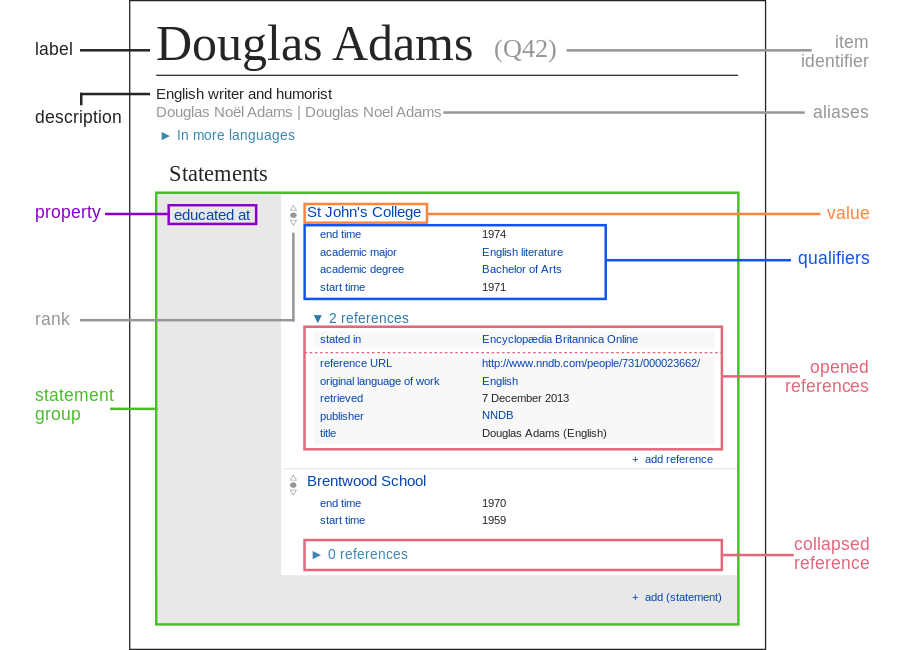
\includegraphics{png/wikidata/File_Datamodel_in_Wikidata.png}

}

\caption{Wikidata is a document-oriented database. This document
connects a lot of knowledge about the late English writer and humorist,
Douglas Adams.}

\end{figure}%

Knowledge graphs connect things in the real world, because their
nodes---in Wikidata, the conceptual document---, represent people,
objects, and their relationships as they are out there, and not as they
are represented by an ``ordinary'' database . The
\href{https://www.wikidata.org/wiki/Q42}{Q42} document about the late
English writer and humorist Douglas Adams connects facts about his life
(birthday, place of birth, time of death), and connects him to his
books, their translations, identifiers to look up these books, and so
on.

Wikidata is a knowledge graph: it connects the concept of Douglas Adams
(\href{https://www.wikidata.org/wiki/Q42}{Q42}), to the concept of his
most quoted humorous episode from his world-famous \emph{Hitchhiker's
Guide to the Galaxy}
(\href{https://www.wikidata.org/wiki/Q25169}{Q25169}) , which is a
similarly structured document about the five books of his series, which
document is further connected in the graph to the concept of the books'
Serbian translation
(\href{https://www.wikidata.org/wiki/Q117279887}{Q117279887}).

Wikidata is not a database but a very useful system for filling up and
keeping many databases in sync worldwide. If your own institutional or
private library has a catalogue, you may have a copy of the
\emph{Hitchhiker's Guide to the Galaxy}; in this case, your catalogue is
likely to have a local, private identifier to your copy of the book.
Imagine your little private catalogue, where you, like the editors of
Wikidata, reserved the \#42 entry to Douglas Adams' book.

\begin{longtable}[]{@{}
  >{\raggedright\arraybackslash}p{(\columnwidth - 4\tabcolsep) * \real{0.2000}}
  >{\raggedright\arraybackslash}p{(\columnwidth - 4\tabcolsep) * \real{0.3000}}
  >{\raggedright\arraybackslash}p{(\columnwidth - 4\tabcolsep) * \real{0.5000}}@{}}
\toprule\noalign{}
\begin{minipage}[b]{\linewidth}\raggedright
Local ID
\end{minipage} & \begin{minipage}[b]{\linewidth}\raggedright
Author
\end{minipage} & \begin{minipage}[b]{\linewidth}\raggedright
Title
\end{minipage} \\
\midrule\noalign{}
\endhead
\bottomrule\noalign{}
\endlastfoot
My-01 & Martell, Yann
(\href{https://www.wikidata.org/wiki/Q13914}{Q13914}) & \emph{Life of
Pi} (\href{https://www.wikidata.org/wiki/Q374204}{Q374204}) \\
\ldots{} & \ldots{} & \ldots{} \\
My-42 & Adams, Douglas (\href{https://www.wikidata.org/wiki/Q42}{Q42}) &
\emph{Hitchhiker's Guide to the Galaxy
(}\href{https://www.wikidata.org/wiki/Q25169}{Q25169}) \\
\ldots{} & \ldots{} & \ldots{} \\
\end{longtable}

If you can connect your \textbf{My-42} entry of \emph{Hitchhiker's Guide
to the Galaxy} with the books' Wikidata entry
\href{https://www.wikidata.org/wiki/Q25169}{Q25169}, you can import a
wealth of information into your private catalogue (the book's metadata,
information about its editions etc.). Furthermore, if you connect the
Wikidata item \href{https://www.wikidata.org/wiki/Q42}{Q42} of the
author Douglas Adams to your catalogue's own entry about the author, you
can import a lot of additional knowledge, for example, information about
his other works, or the end term of these books' copyright protection,
after which they will become public domain and they will be free to copy
and distribute.

In Wikidata, each item has a unique,
\href{https://en.wikipedia.org/wiki/Persistent_identifier}{persistent
identifier}, a positive integer number, prefixed with the upper-case
letter Q, known as a ``QID''.Global information systems like to anchor
authoritative information about people, books, musical works, and other
important things to persistent identifiers. For example, in VIAF, the
authority file that keeps information synchronised across national
libraries, Douglas Adams' persistent identifier is
\href{https://viaf.org/viaf/113230702/}{113230702}, whereas in the
Portuguese National Library it is
\href{http://id.bnportugal.gov.pt/aut/catbnp/68537}{68537}. Wikidata is
particularly useful because it serves as an ``identity broker'', and
this linking information can be retrieved directly from Douglas Adams'
\href{https://www.wikidata.org/wiki/Q42}{Q42} page.

\begin{center}
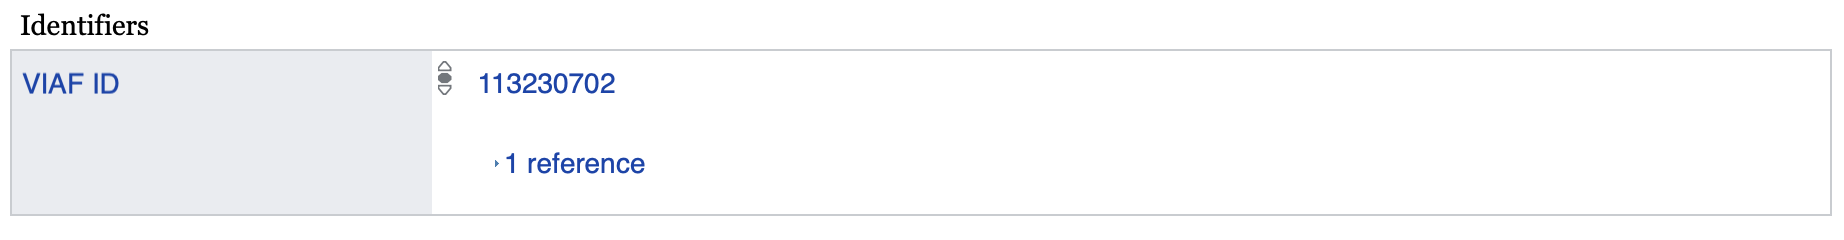
\includegraphics{png/wikidata-tutorial/Douglas-Adams_VIAF-identifier.png}
\end{center}

\begin{center}
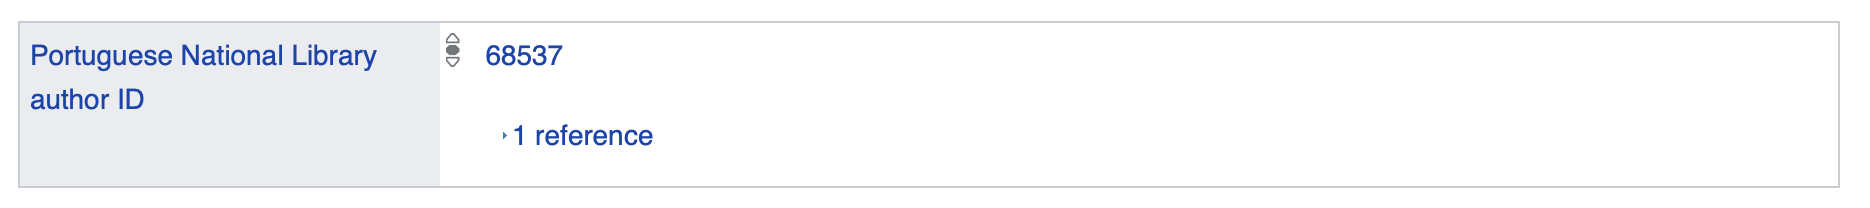
\includegraphics{png/wikidata-tutorial/Douglas-Adams_portugal-national-library-identifier.png}
\end{center}

\subsection{Getting started with
Wikidata}\label{sec-getting-started-wikidata}

\begin{tcolorbox}[enhanced jigsaw, opacityback=0, bottomrule=.15mm, rightrule=.15mm, toptitle=1mm, breakable, colbacktitle=quarto-callout-tip-color!10!white, colback=white, title=\textcolor{quarto-callout-tip-color}{\faLightbulb}\hspace{0.5em}{Tip}, leftrule=.75mm, toprule=.15mm, left=2mm, arc=.35mm, colframe=quarto-callout-tip-color-frame, coltitle=black, titlerule=0mm, bottomtitle=1mm, opacitybacktitle=0.6]

Wikidata, the world's biggest open knowledge graph uses the same
Wikibase software that we use. Editing entries on Wikidata is identical
to editing Wikibase. Depending on your needs, you can follow our
tutorial on working with the public, global, shared Wikidata or one of
our private (Wikibase) versions. See
Section~\ref{sec-first-edits-wikibase}.

\end{tcolorbox}

\subsection{First editing on Wikidata}\label{sec-first-edits-wikidata}

In the example below, you see an \texttt{Item} page. An \texttt{Item} is
a person, a living thing, a group of person, or an inanimate object
(thing). Each page collects knowledge in the form of \texttt{Statements}
about this person or thing.

\subsection{Definitions and their
translations}\label{definitions-and-their-translations}

Each \texttt{Item} page has a \texttt{label}, in this case,
\texttt{music\ artist}, which is a short title to the page. It also has
a \texttt{description} about the meaning of a \texttt{music\ artist}. It
may also have \texttt{alias} fields, which show that a
\texttt{music\ artist} is often just simply called a \texttt{musician}.

Probably the first and simplest editing is when you add a new
translation of a \texttt{label}, a new \texttt{description} of the
person or thing, or a new \texttt{alias} (an alternate name, a synonym
or a pseudonym.)

In this example, the Hungarian translation is changed from ``zenei
előadóművész'', which refers to only performers, to the broader
occupation of \emph{zeneművész}, which includes componists and
conductors, too, and a new description is added to a Wikidata page that
has no good Hungarian description.

\begin{center}
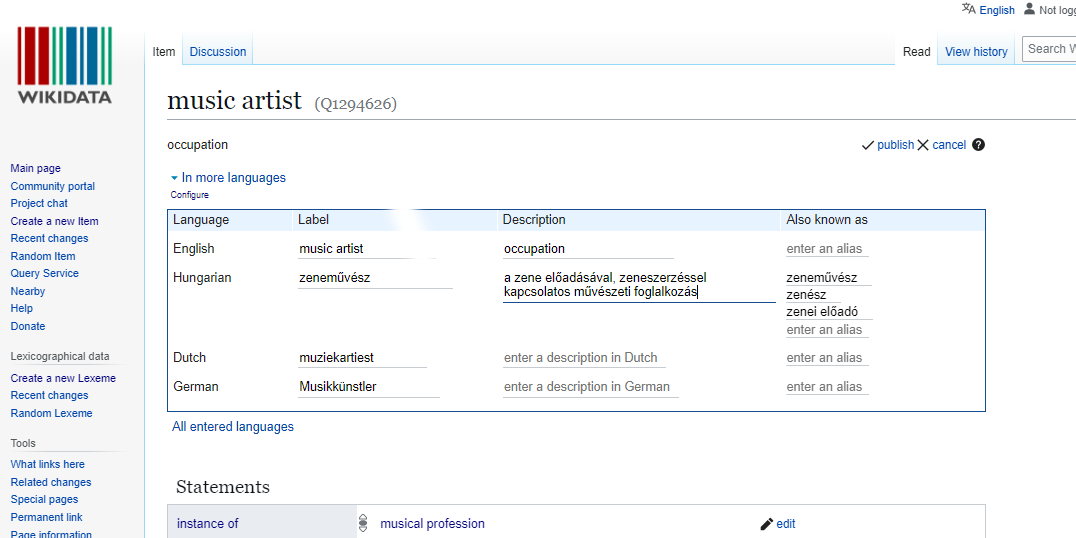
\includegraphics{png/wikidata/add_new_translation_wikidata_2x1.png}
\end{center}

\begin{tcolorbox}[enhanced jigsaw, opacityback=0, bottomrule=.15mm, rightrule=.15mm, toptitle=1mm, breakable, colbacktitle=quarto-callout-caution-color!10!white, colback=white, title=\textcolor{quarto-callout-caution-color}{\faFire}\hspace{0.5em}{Caution}, leftrule=.75mm, toprule=.15mm, left=2mm, arc=.35mm, colframe=quarto-callout-caution-color-frame, coltitle=black, titlerule=0mm, bottomtitle=1mm, opacitybacktitle=0.6]

You should only make changes on Wikidata when you \emph{really} know
what you do. Our Wikibase instances (private copies of Wikidata) allow
you place to experiment and learn in a near-identical user interface,
where only a few buttons are different from Wikidata. See
Section~\ref{sec-first-edits-wikibase}.

\end{tcolorbox}

\subsubsection{Global Identities}\label{global-identities}

Mr and Mrs Barasits, a.k.a. \texttt{János\ Barasits} (1859-1935) and his
wife, \texttt{Barasits,\ Jánosné}, born Pichler, Kornélia, were
prominent postcard producers and publishers at the beginning of the 20th
century. They produced plenty of beautiful postcards.

In the 1920s and 1930s, the authors' right (\textasciitilde copyright)
protection of photographs and postcards was relatively short, only 15
years, so their postcards went into the public domain in terms of
copying long ago. Plenty of their beautiful works are out there on the
internet, but it is very hard to put them into a collection, because
most databases know next to nothing about the identities of these
creators and their creations.

Unfortunately, you cannot find their name in the most commonly used
authority controls, i.e., VIAF or ISNI. Writing to VIAF is only possible
via member institutions, and ISNI costs money. A temporary solution is
to create a Wikidata QID for János Barasits
(\href{https://www.wikidata.org/wiki/Q124423018}{Q124423018}), until
somebody registers his name into VIAF. With this entry, it will be
easier to find further postcards from them, or other information about
them all over the world!

Writing in Wikidata is free for all and subject to community review. If
you read this tutorial, please pledge to record new persons (or other
items) into Wikidata, only if your knowledge is solid. You can verify
the information needed through proper research.

\subsubsection{Create a Wikidata Item}\label{create-a-wikidata-item}

In this tutorial, you can learn how to create a new item on Wikidata.
Countless web and AI applications and millions of people use Wikidata,
so in the beginning it is recommended to not experiment with it in the
live system. Wikidata has a
\href{https://www.wikidata.org/wiki/Wikidata:Sandbox}{Sandbox} for
practising. We recommend using it as a first step. If you work with
Wikibase, particularly with Reprex's OpenCollections, you will have
access to a similar sandbox. It will be prefilled with data, concepts,
and properties suitable for your learning needs, often going beyond what
you would find in the public Wikidata.

Let's see how you can create your own János Barasits item.

You can see how creating a new item looks like in the system:

\begin{center}
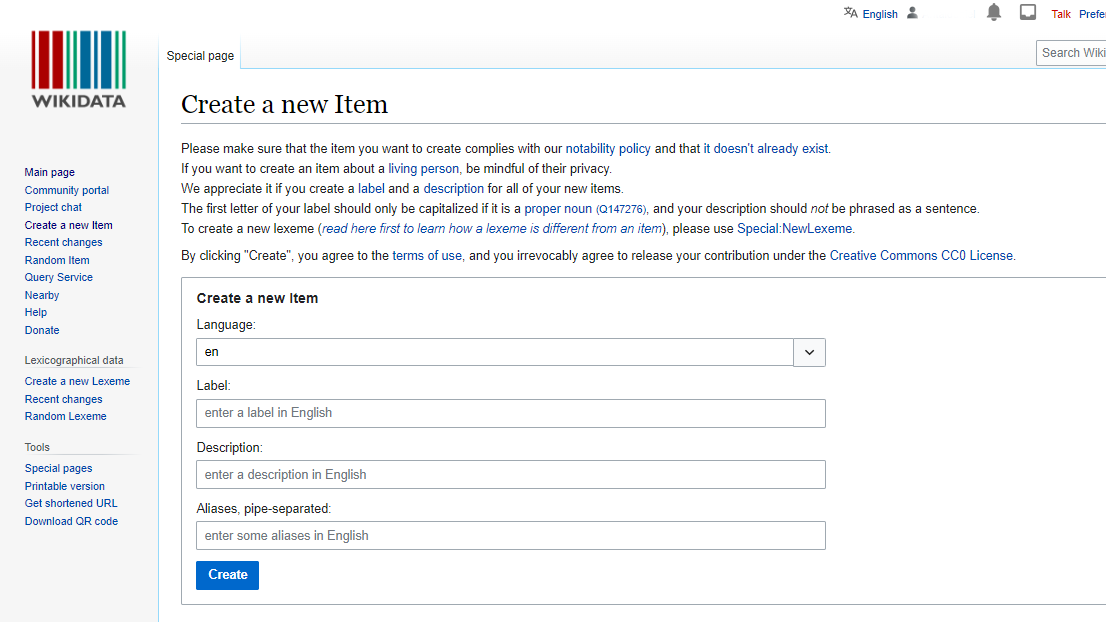
\includegraphics{png/wikidata-tutorial/wikidata-create-new-item-20240204.png}
\end{center}

The first step in creating an item (in this case an item for János
Barasits) is providing the two most important information for an item,
which is the \texttt{Label} and the \texttt{Description}.

The \texttt{Label} is the name of the item (in our case the label of the
item will be ``János Barasits'').

The \texttt{Description} contains a short explanation of our item (in
our case the description for the item will be ``Hungarian postcard maker
and publisher).

\texttt{Aliases} are alternative names for the item.

After creating the item with the basic information of \texttt{Label} and
\texttt{Description} we can weave this information entry into the
knowledge graph. At this point, \texttt{János\ Barasits} could be a
person, it could be a book titled after the person, or a photo of the
person. Connecting János Barasits to other entities, such as the concept
of a human being, will allow other people and their computer systems to
understand that we are talking about a person here.You can do that by
creating ``statements'' (See Tip~\ref{tip-statement}.)

The property ``instance of'' defines the class our item is a particular
example or member of. In this case we would like to make a statement
about our item ``János Barasits'' defining with the property ``instance
of'' that he is a member of the ``human'' class.

\begin{center}
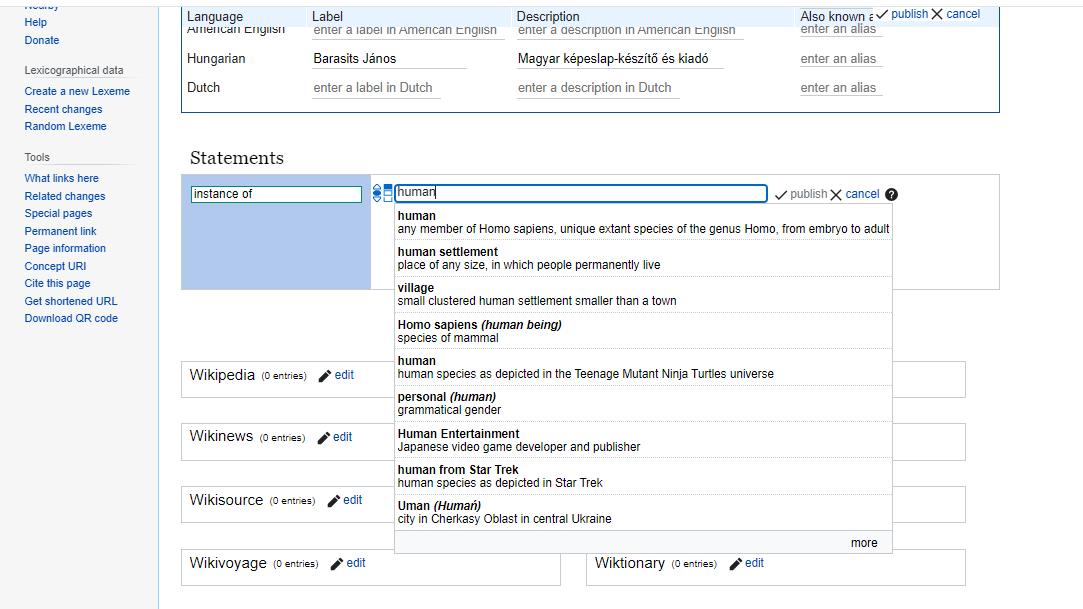
\includegraphics{png/wikidata-tutorial/wikidata-create-new-item-Janos-Barasits-20240204-2.png}
\end{center}

Through the sandbox explore the different type of properties and
statements. Add a few basic statement to your new item:

\begin{itemize}
\tightlist
\item
  János Barasits is a human---his gender was male---he was born in 1859
  (with the precision of a year only)---he died in 1935.
\end{itemize}

It should look similar to this:

\begin{center}
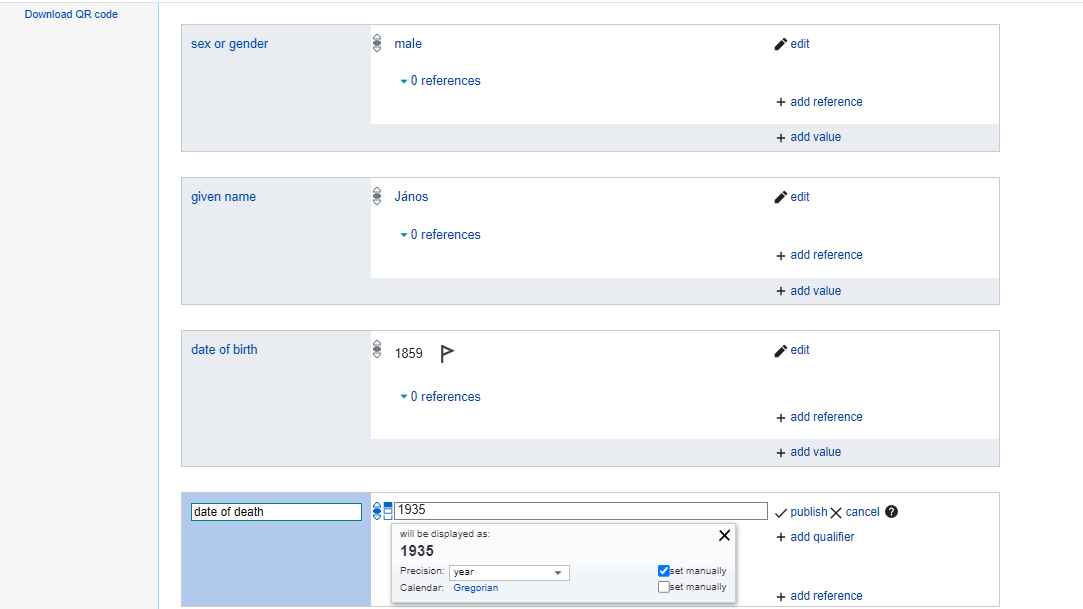
\includegraphics{png/wikidata-tutorial/wikidata-create-new-item-Janos-Barasits-20240204-3.png}
\end{center}

To see another example on how useful knowledge graphs can be consider
the following. The four characters, \texttt{1935} can be understood as a
number for most readers, but such a data point without a defined meaning
is useless. In a basic database you would see 1935 and know that it is a
number. However, in knowledge graphs, like here on Wikidata, when we add
the ``metadata'', and we connect 1935 to the definition of
\texttt{date\ of\ death}, we add a meaning (``semantics'') to the number
1935. Now, 1935 is not only a number but also a date of someone's death.

The definition of date of death is useful in itself, but in a knowledge
base, we can do even more with this piece of information. With this
information we can combine the fact that in Europe the copyright
protection term of people's creation runs up to 70 years after their
death. Thus, a knowledge base can infer the fact that currently János
Barasits's postcards are out of copyright and they can be freely copied
and distributed!

Here is a very basic Wikidata page for
\href{https://www.wikidata.org/wiki/Q124423018}{János Barasits}. What is
very important, is that we have a globally unique identifier,
\texttt{Q124423018} that uniquely identifies him as a human. If you have
a collection of postcards (digitals or analogue, vintage physical
objects), connecting your own database with \texttt{Q124423018} will
help you to import the knowledge of the expired copyright protection
term; it will help you finding other out-of-copyright scanned copies of
Barasits' postcards; it will be easier to connect to other collections
that hold items from them, and so on.

\begin{tcolorbox}[enhanced jigsaw, opacityback=0, bottomrule=.15mm, rightrule=.15mm, toptitle=1mm, breakable, colbacktitle=quarto-callout-tip-color!10!white, colback=white, title=\textcolor{quarto-callout-tip-color}{\faLightbulb}\hspace{0.5em}{Further tutorial}, leftrule=.75mm, toprule=.15mm, left=2mm, arc=.35mm, colframe=quarto-callout-tip-color-frame, coltitle=black, titlerule=0mm, bottomtitle=1mm, opacitybacktitle=0.6]

Working with Persons in Wikibase ---
\href{https://opencollections.net/documents/tutorials/wikibase_persons_tutorial.html\#/title-slide}{Adding
persons as named entities to Wikidata or a Wikibase}

\end{tcolorbox}

\subsection{Retrieve an item from
Wikidata}\label{retrieve-an-item-from-wikidata}

Many internal enterprise resource systems or APIs use SQL, a 50+
year-old data query language. SQL is the lingua franca of relational
database systems; you may be familiar with it. Can you query Wikidata in
SQL?

Not exactly. It requires a different querying language, which was
developed for knowledge graphs. It is called SPARQL because it is
similar to SQL, but they are rather distant cousins.

While SQL is widely used, it does have a significant limitation: your
query scripts are specific to one database system or API. What works in
your internal catalogue may not function in another organisation's. If
you've written a script to update your data from a specific web API, it
doesn't guarantee that the script will be compatible with another API.
Furthermore, it's not future-proof: if the API owner (or your database
manager) makes even a slight adjustment to the system, you may need to
modify or rewrite your retrieval code.

Remember, the significant advantage of Wikidata and other open knowledge
graphs is that millions of people work on improvements and extensions
daily. This means that an SQL request would be outdated every day.
Instead of SQL, SPARQL queries do not look for cells in data tables, but
they use intelligent knowledge to find the cells containing data about
what you need. In SQL, you need to know which table contains people's
birthdays and death dates to find out the year when János Barasits died.
In SPARQL, you are looking for the cell that contains the date of death
for the human known as János Barasits.

\subsection{SPARQL basics}\label{sec-sparql}

SPARQL, pronounced `sparkle', is the standard query language and
protocol for Linked Open Data and RDF databases. Having been designed to
query a great variety of data, it can efficiently extract information
hidden in non-uniform data and store it in various formats and sources.
The SPARQL standard is designed and endorsed by the World Wide Web
Consortium and helps users and developers focus on what they would like
to know instead of how a database is organised. With SPARQL, you can
access many large open knowledge resources, like the EU Open Data Portal
(see \href{https://data.europa.eu/data/sparql?locale=en}{here}), the
Eurostat data warehouse, or Wikidata (turorial
\href{https://www.wikidata.org/wiki/Wikidata:SPARQL_tutorial}{here}), or
the knowledge basis of the Dutch heritage organisations, including the
Rijksmuseum (see
\href{https://data.netwerkdigitaalerfgoed.nl/Rijksmuseum/collection/sparql}{here}).

Our data curators must be able to run SPARQL queries and make elementary
modifications to them. Because we often import very large datasets, it
would be very difficult to manually control every record on the
graphical user interface. We use pre-written SPARQL queries (the data
curator is expected to run via a simple URL link, perhaps modifying a
class's QID or a property's PID) that serve as so-called \emph{unit
tests}. These queries programmed by Reprex allow simple tests like
these:

\begin{itemize}
\tightlist
\item[$\boxtimes$]
  If the curator gave us 5432 person records, we have 5432 persons in
  the Reprexbase instance;
\item[$\boxtimes$]
  If the gender breakup of a person's records is 2834:2598, the instance
  results in exactly the same persons of two genders (assuming that no
  third gender is used in the original data.)
\item[$\boxtimes$]
  If we received data on Ján Levoslav Bella's Symphony in B minor, the
  publication year is 1982.
\end{itemize}

A simple SPARQL query looks like this:

\begin{Shaded}
\begin{Highlighting}[]
\NormalTok{SELECT ?a ?b ?c}
\NormalTok{WHERE}
\NormalTok{\{}
\NormalTok{  x y ?a.}
\NormalTok{  m n ?b.}
\NormalTok{  ?b f ?c.}
\NormalTok{\}}
\end{Highlighting}
\end{Shaded}

Suppose we want to list all children of the baroque composer Johann
Sebastian Bach. Using pseudo-elements like in the queries above, how
would you write that query?

Hopefully you got something like this:

\begin{Shaded}
\begin{Highlighting}[]
\NormalTok{SELECT ?child}
\NormalTok{WHERE}
\NormalTok{\{}
  \CommentTok{\#  child "has parent" Bach}
\NormalTok{  ?child parent Bach.}
  \CommentTok{\# (note: everything after a ‘\#’ is a comment and ignored by WDQS.)}
\NormalTok{\}}
\end{Highlighting}
\end{Shaded}

or this,

\begin{Shaded}
\begin{Highlighting}[]
\NormalTok{SELECT ?child}
\NormalTok{WHERE}
\NormalTok{\{}
  \CommentTok{\# child "has father" Bach }
\NormalTok{  ?child father Bach. }
\NormalTok{\}}
\end{Highlighting}
\end{Shaded}

or this,

\begin{Shaded}
\begin{Highlighting}[]
\NormalTok{SELECT ?child}
\NormalTok{WHERE}
\NormalTok{\{}
  \CommentTok{\#  Bach "has child" child}
\NormalTok{  Bach child ?child.}
\NormalTok{\}}
\end{Highlighting}
\end{Shaded}

The first two triples say that the ?child must have the parent/father
Bach; the third says that Bach must have the child ?child. Let's go with
the second one for now.

So what remains to be done in order to turn this into a proper WDQS
query? On Wikidata, items and properties are not identified by
human-readable names like ``father'' (property) or ``Bach'' (item). (For
good reason: ``Johann Sebastian Bach'' is also the name of a German
painter, and ``Bach'' might also refer to the surname, the French
commune, the Mercury crater, etc.) Instead, Wikidata items and
properties are assigned an identifier. To find the identifier for an
item, we search for the item and copy the Q-number of the result that
looks like it is the item we are looking for (based on the description,
for example). To find the identifier for a property, we do the same, but
search for ``P:search term'' instead of just ``search term'', which
limits the search to properties. This tells us that the famous composer
Johann Sebastian Bach is \texttt{Q1339}, and the property to designate
an item's father is \texttt{P:22}.

And last but not least, we need to include prefixes. For simple WDQS
triples, items should be prefixed with \texttt{wd:}, and properties with
\texttt{wdt:}. (But this only applies to fixed values -- variables don't
get a prefix!)

Putting this together, we arrive at our first proper WDQS query:

\begin{Shaded}
\begin{Highlighting}[]
\NormalTok{SELECT ?child}
\NormalTok{WHERE}
\NormalTok{\{}
\CommentTok{\# ?child  father   Bach}
\NormalTok{  ?child wdt}\SpecialCharTok{:}\NormalTok{P22 wd}\SpecialCharTok{:}\NormalTok{Q1339.}
\NormalTok{\}}
\end{Highlighting}
\end{Shaded}

Try the first query:

\begin{figure}[H]

{\centering 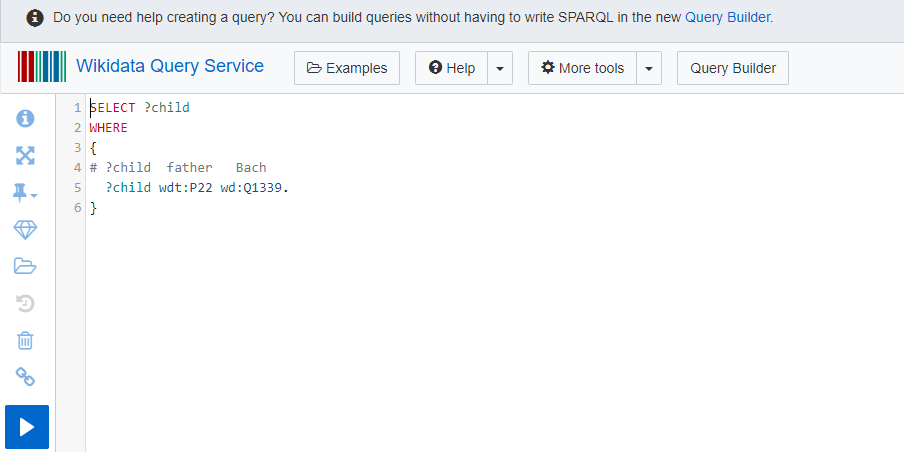
\includegraphics{png/wikidata-tutorial/sparql-example-bach-children-without-labels.png}

}

\caption{Click on the image to try it out live on the Wikidata SPARQL
Endpoint. The query will run if you press the ▶ sign on the endpoint in
the bottom left corner.}

\end{figure}%

\begin{tcolorbox}[enhanced jigsaw, opacityback=0, bottomrule=.15mm, rightrule=.15mm, toptitle=1mm, breakable, colbacktitle=quarto-callout-tip-color!10!white, colback=white, title=\textcolor{quarto-callout-tip-color}{\faLightbulb}\hspace{0.5em}{Tip \ref*{tip-timeout}: Query timeout limit reached}, leftrule=.75mm, toprule=.15mm, left=2mm, arc=.35mm, colframe=quarto-callout-tip-color-frame, coltitle=black, titlerule=0mm, bottomtitle=1mm, opacitybacktitle=0.6]

\quartocallouttip{tip-timeout} 

If you recieve a \texttt{Query\ timeout\ limit\ reached} error message,
it is likely that you tried to make a query that resulted in too many
responses, and you ran out of memory or some other resource. This can be
most likely solved with some kind of limitation on the number of
possible answer rows that you get.

The simplest limitation is adding a last line to your query:
\texttt{limit\ 10}, which limits the descendants of J.S. Back to the
first 10 people (see the previous example with
\href{https://query.wikidata.org/\#SELECT\%20\%3Fchild\%0AWHERE\%0A\%7B\%0A\%23\%20\%3Fchild\%20\%20father\%20\%20\%20Bach\%0A\%20\%20\%3Fchild\%20wdt\%3AP22\%20wd\%3AQ1339.\%0A\%7D\%20limit\%2010}{this
limit}.)

\end{tcolorbox}

The first querry will provide you with identifiers, which is great if
you are a programmer and you are wiring your database to Wikidata, but
less impressive if you are getting familiar with SPARQL and you want to
see clearly the fruits of your work.

Luckily, Wikidata has a human-friendly extension to SPARQL. If you add
the following command to your query:
\texttt{SERVICE\ wikibase:label\ \{\ bd:serviceParam\ wikibase:language\ "{[}AUTO\_LANGUAGE{]}".}somewhere
within the \texttt{WHERE} clause, you get additional variables: For
every variable \texttt{?foo} in your query, you now also have a variable
\texttt{?fooLabel}, which contains the label of the item behind
\texttt{?foo}.

If you add this to the \texttt{SELECT} clause, you get the item as well
as its label:

\begin{Shaded}
\begin{Highlighting}[]
\NormalTok{SELECT ?child ?childLabel}
\NormalTok{WHERE}
\NormalTok{\{}
\CommentTok{\# ?child  father   Bach}
\NormalTok{  ?child wdt}\SpecialCharTok{:}\NormalTok{P22 wd}\SpecialCharTok{:}\NormalTok{Q1339.}
\NormalTok{  SERVICE wikibase}\SpecialCharTok{:}\NormalTok{label \{ bd}\SpecialCharTok{:}\NormalTok{serviceParam wikibase}\SpecialCharTok{:}\NormalTok{language }\StringTok{"[AUTO\_LANGUAGE]"}\NormalTok{. \}}
\NormalTok{\}}
\end{Highlighting}
\end{Shaded}

\begin{figure}[H]

{\centering 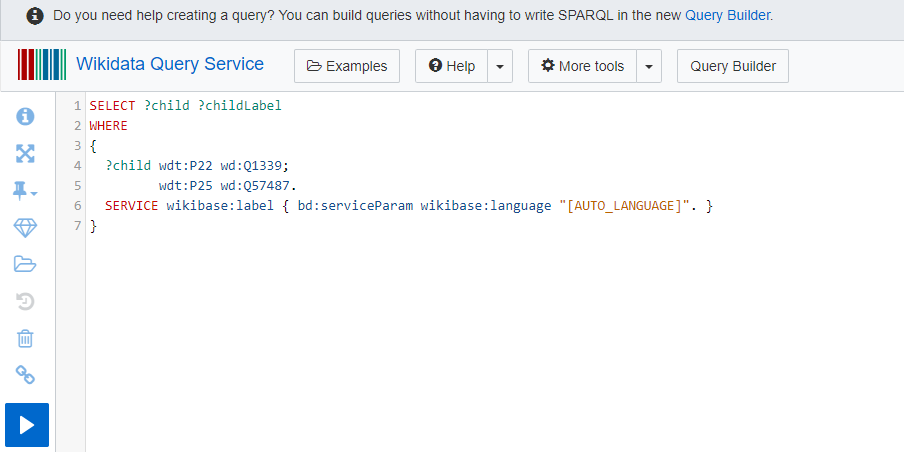
\includegraphics{png/wikidata-tutorial/sparql-example-bach-children-with-labels.png}

}

\caption{Click on the image to try it out live on the Wikidata SPARQL
Endpoint. The query will run if you press the ▶ sign on the endpoint in
the bottom left corner↗.}

\end{figure}%

Try running that query -- you should see not only the item numbers, but
also the names of the various children.

\begin{longtable}[]{@{}
  >{\raggedright\arraybackslash}p{(\columnwidth - 2\tabcolsep) * \real{0.6111}}
  >{\raggedright\arraybackslash}p{(\columnwidth - 2\tabcolsep) * \real{0.3889}}@{}}
\toprule\noalign{}
\begin{minipage}[b]{\linewidth}\raggedright
child
\end{minipage} & \begin{minipage}[b]{\linewidth}\raggedright
childLabel
\end{minipage} \\
\midrule\noalign{}
\endhead
\bottomrule\noalign{}
\endlastfoot
\href{http://www.wikidata.org/entity/Q76428}{wd:Q57225} & Johann
Christoph Friedrich Bach \\
\href{http://www.wikidata.org/entity/Q76428}{wd:Q76428} & Carl Philipp
Emanuel Bach \\
\ldots{} & \\
\end{longtable}

\subsection{Pre-filter Wikidata}\label{pre-filter-wikidata}

When you work with OpenCollections or Wikibase, you may want to
synchronize your knowledge graph with Wikidata. A straightforward way to
do this is to import a part of the Wikidata knowledge graph into your
instance.

Imagine you would like to copy the definition of a human, Béla Bartók,
to your Wikibase instances. The following querry

\begin{Shaded}
\begin{Highlighting}[]
\NormalTok{SELECT DISTINCT ?itemLabel ?itemLabelLang ?itemDescription ?itemDescriptionLang ?aliases ?aliasesLang WHERE \{}
\NormalTok{  wd}\SpecialCharTok{:}\NormalTok{Q83326 rdfs}\SpecialCharTok{:}\NormalTok{label ?itemLabel ;}
\NormalTok{            schema}\SpecialCharTok{:}\NormalTok{description ?itemDescription .}
\NormalTok{  OPTIONAL \{}
\NormalTok{    wd}\SpecialCharTok{:}\NormalTok{Q83326 skos}\SpecialCharTok{:}\NormalTok{altLabel ?aliases .}
    \FunctionTok{BIND}\NormalTok{(}\FunctionTok{LANG}\NormalTok{(?aliases) AS ?aliasesLang)}
\NormalTok{  \}}
  \FunctionTok{BIND}\NormalTok{(}\FunctionTok{LANG}\NormalTok{(?itemLabel) AS ?itemLabelLang)}
  \FunctionTok{BIND}\NormalTok{(}\FunctionTok{LANG}\NormalTok{(?itemDescription) AS ?itemDescriptionLang)}
  \FunctionTok{FILTER}\NormalTok{(?itemLabelLang }\FunctionTok{IN}\NormalTok{ (}\StringTok{"en"}\NormalTok{, }\StringTok{"de"}\NormalTok{, }\StringTok{"hu"}\NormalTok{, }\StringTok{"sk"}\NormalTok{, }\StringTok{"lt"}\NormalTok{, }\StringTok{"bg"}\NormalTok{))}
  \FunctionTok{FILTER}\NormalTok{(?itemDescriptionLang }\FunctionTok{IN}\NormalTok{ (}\StringTok{"en"}\NormalTok{, }\StringTok{"de"}\NormalTok{, }\StringTok{"hu"}\NormalTok{, }\StringTok{"sk"}\NormalTok{, }\StringTok{"lt"}\NormalTok{, }\StringTok{"bg"}\NormalTok{))}
  \FunctionTok{FILTER}\NormalTok{(?aliasesLang }\FunctionTok{IN}\NormalTok{ (}\StringTok{"en"}\NormalTok{, }\StringTok{"de"}\NormalTok{, }\StringTok{"hu"}\NormalTok{, }\StringTok{"sk"}\NormalTok{, }\StringTok{"lt"}\NormalTok{, }\StringTok{"bg"}\NormalTok{))}
\NormalTok{\}}
\end{Highlighting}
\end{Shaded}

\href{https://query.wikidata.org/\#SELECT\%20DISTINCT\%20\%3FitemLabel\%20\%3FitemLabelLang\%20\%3FitemDescription\%20\%3FitemDescriptionLang\%20\%3Faliases\%20\%3FaliasesLang\%20WHERE\%20\%7B\%0A\%20\%20wd\%3AQ83326\%20rdfs\%3Alabel\%20\%3FitemLabel\%20\%3B\%0A\%20\%20\%20\%20\%20\%20\%20\%20\%20\%20\%20\%20schema\%3Adescription\%20\%3FitemDescription\%20.\%0A\%20\%20OPTIONAL\%20\%7B\%0A\%20\%20\%20\%20wd\%3AQ83326\%20skos\%3AaltLabel\%20\%3Faliases\%20.\%0A\%20\%20\%20\%20BIND\%28LANG\%28\%3Faliases\%29\%20AS\%20\%3FaliasesLang\%29\%0A\%20\%20\%7D\%0A\%20\%20BIND\%28LANG\%28\%3FitemLabel\%29\%20AS\%20\%3FitemLabelLang\%29\%0A\%20\%20BIND\%28LANG\%28\%3FitemDescription\%29\%20AS\%20\%3FitemDescriptionLang\%29\%0A\%20\%20FILTER\%28\%3FitemLabelLang\%20IN\%20\%28\%22en\%22\%2C\%20\%22de\%22\%2C\%20\%22hu\%22\%2C\%20\%22sk\%22\%2C\%20\%22lt\%22\%2C\%20\%22bg\%22\%29\%29\%0A\%20\%20FILTER\%28\%3FitemDescriptionLang\%20IN\%20\%28\%22en\%22\%2C\%20\%22de\%22\%2C\%20\%22hu\%22\%2C\%20\%22sk\%22\%2C\%20\%22lt\%22\%2C\%20\%22bg\%22\%29\%29\%0A\%20\%20FILTER\%28\%3FaliasesLang\%20IN\%20\%28\%22en\%22\%2C\%20\%22de\%22\%2C\%20\%22hu\%22\%2C\%20\%22sk\%22\%2C\%20\%22lt\%22\%2C\%20\%22bg\%22\%29\%29\%0A\%7D}{Try
it out↗}

\begin{itemize}
\item[$\boxtimes$]
  You can modify the querry. In Line 3, the \texttt{wd:Q83326}
  identifies the QID for Béla Bartók. Try it out with
  \texttt{wd:\textasciigrave{}\textasciigrave{}28104185}!
\item[$\boxtimes$]
  We asked the labelling in six languages. You can use
  \texttt{IN\ ("en",\ "de")} or even \texttt{IN\ ("de")} if you want to
  reduce the number of languages or change the language codes.
\item[$\square$]
  If you reach the query timeout, try to limit your search (see (See
  Tip~\ref{tip-timeout}.)
\end{itemize}

You would like to copy property definitions to your Wikibase instance.
The following code will provide you the necessary information (without
additional statements) about the property \texttt{wd:P31}---a very
important property for data modelling.

\begin{Shaded}
\begin{Highlighting}[]
\NormalTok{SELECT ?property ?propertyLabel ?dataType ?propertyDescription ?lang ?alias WHERE \{}
\NormalTok{  VALUES ?property \{ wd}\SpecialCharTok{:}\NormalTok{P31 \}  }\CommentTok{\# Replace these IDs with the property IDs you are interested in}
\NormalTok{  ?property a wikibase}\SpecialCharTok{:}\NormalTok{Property .}
\NormalTok{  ?property wikibase}\SpecialCharTok{:}\NormalTok{propertyType ?dataType .}

  \CommentTok{\# Fetch labels in the specified languages}
\NormalTok{  ?property rdfs}\SpecialCharTok{:}\NormalTok{label ?propertyLabel .}
  \FunctionTok{BIND}\NormalTok{(}\FunctionTok{LANG}\NormalTok{(?propertyLabel) AS ?lang)}
  \FunctionTok{FILTER}\NormalTok{(?lang }\FunctionTok{IN}\NormalTok{ (}\StringTok{"en"}\NormalTok{, }\StringTok{"fr"}\NormalTok{, }\StringTok{"sk"}\NormalTok{, }\StringTok{"hu"}\NormalTok{, }\StringTok{"bg"}\NormalTok{, }\StringTok{"lt"}\NormalTok{))  }\CommentTok{\# Replace these your languages}
  \FunctionTok{BIND}\NormalTok{(}\FunctionTok{IF}\NormalTok{(?}\AttributeTok{lang =} \StringTok{"en"}\NormalTok{, }\DecValTok{1}\NormalTok{, }\DecValTok{2}\NormalTok{) AS ?labelRank)}

  \CommentTok{\# Fetch descriptions in the specified languages}
\NormalTok{  OPTIONAL \{}
\NormalTok{    ?property schema}\SpecialCharTok{:}\NormalTok{description ?propertyDescription .}
    \FunctionTok{FILTER}\NormalTok{(}\FunctionTok{LANG}\NormalTok{(?propertyDescription) }\FunctionTok{IN}\NormalTok{ (}\StringTok{"en"}\NormalTok{, }\StringTok{"fr"}\NormalTok{, }\StringTok{"sk"}\NormalTok{, }\StringTok{"hu"}\NormalTok{, }\StringTok{"bg"}\NormalTok{, }\StringTok{"lt"}\NormalTok{))}
    \FunctionTok{FILTER}\NormalTok{(}\FunctionTok{LANG}\NormalTok{(?propertyDescription) }\OtherTok{=}\NormalTok{ ?lang)  }\CommentTok{\# Ensure matching languages}
\NormalTok{  \}}
  \CommentTok{\# Fetch aliases in the specified languages}
\NormalTok{  OPTIONAL \{}
\NormalTok{  ?property skos}\SpecialCharTok{:}\NormalTok{altLabel ?alias .}
  \FunctionTok{FILTER}\NormalTok{(}\FunctionTok{LANG}\NormalTok{(?alias) }\FunctionTok{IN}\NormalTok{ (}\StringTok{"en"}\NormalTok{, }\StringTok{"fr"}\NormalTok{, }\StringTok{"sk"}\NormalTok{, }\StringTok{"hu"}\NormalTok{, }\StringTok{"bg"}\NormalTok{, }\StringTok{"lt"}\NormalTok{))}
  \FunctionTok{FILTER}\NormalTok{(}\FunctionTok{LANG}\NormalTok{(?alias) }\OtherTok{=}\NormalTok{ ?lang)  }\CommentTok{\# Ensure matching languages}
\NormalTok{  \}}

\NormalTok{\}}
\NormalTok{ORDER BY ?labelRank ?lang}
\end{Highlighting}
\end{Shaded}

\href{https://query.wikidata.org/\#SELECT\%20\%3Fproperty\%20\%3FpropertyLabel\%20\%3FdataType\%20\%3FpropertyDescription\%20\%3Flang\%20\%3Falias\%20WHERE\%20\%7B\%0A\%20\%20VALUES\%20\%3Fproperty\%20\%7B\%20wd\%3AP31\%20\%7D\%20\%20\%23\%20Replace\%20these\%20IDs\%20with\%20the\%20property\%20IDs\%20you\%20are\%20interested\%20in\%0A\%20\%20\%3Fproperty\%20a\%20wikibase\%3AProperty\%20.\%0A\%20\%20\%3Fproperty\%20wikibase\%3ApropertyType\%20\%3FdataType\%20.\%0A\%0A\%20\%20\%23\%20Fetch\%20labels\%20in\%20the\%20specified\%20languages\%0A\%20\%20\%3Fproperty\%20rdfs\%3Alabel\%20\%3FpropertyLabel\%20.\%0A\%20\%20BIND\%28LANG\%28\%3FpropertyLabel\%29\%20AS\%20\%3Flang\%29\%0A\%20\%20FILTER\%28\%3Flang\%20IN\%20\%28\%22en\%22\%2C\%20\%22fr\%22\%2C\%20\%22sk\%22\%2C\%20\%22hu\%22\%2C\%20\%22bg\%22\%2C\%20\%22lt\%22\%29\%29\%0A\%20\%20BIND\%28IF\%28\%3Flang\%20\%3D\%20\%22en\%22\%2C\%201\%2C\%202\%29\%20AS\%20\%3FlabelRank\%29\%0A\%0A\%20\%20\%23\%20Fetch\%20descriptions\%20in\%20the\%20specified\%20languages\%0A\%20\%20OPTIONAL\%20\%7B\%0A\%20\%20\%20\%20\%3Fproperty\%20schema\%3Adescription\%20\%3FpropertyDescription\%20.\%0A\%20\%20\%20\%20FILTER\%28LANG\%28\%3FpropertyDescription\%29\%20IN\%20\%28\%22en\%22\%2C\%20\%22fr\%22\%2C\%20\%22sk\%22\%2C\%20\%22hu\%22\%2C\%20\%22bg\%22\%2C\%20\%22lt\%22\%29\%29\%0A\%20\%20\%20\%20FILTER\%28LANG\%28\%3FpropertyDescription\%29\%20\%3D\%20\%3Flang\%29\%20\%20\%23\%20Ensure\%20matching\%20languages\%0A\%20\%20\%7D\%0A\%20\%20\%23\%20Fetch\%20aliases\%20in\%20the\%20specified\%20languages\%0A\%20\%20OPTIONAL\%20\%7B\%0A\%20\%20\%3Fproperty\%20skos\%3AaltLabel\%20\%3Falias\%20.\%0A\%20\%20FILTER\%28LANG\%28\%3Falias\%29\%20IN\%20\%28\%22en\%22\%2C\%20\%22fr\%22\%2C\%20\%22sk\%22\%2C\%20\%22hu\%22\%2C\%20\%22bg\%22\%2C\%20\%22lt\%22\%29\%29\%0A\%20\%20FILTER\%28LANG\%28\%3Falias\%29\%20\%3D\%20\%3Flang\%29\%20\%20\%23\%20Ensure\%20matching\%20languages\%0A\%20\%20\%7D\%0A\%0A\%7D\%0AORDER\%20BY\%20\%3FlabelRank\%20\%3Flang}{Try
it out↗}

The same query without
\href{https://query.wikidata.org/\#SELECT\%20\%3Fproperty\%20\%3FpropertyLabel\%20\%3FdataType\%20\%3FpropertyDescription\%20\%3Flang\%20WHERE\%20\%7B\%0A\%20\%20VALUES\%20\%3Fproperty\%20\%7B\%20wd\%3AP31\%20\%7D\%20\%20\%23\%20Replace\%20these\%20IDs\%20with\%20the\%20property\%20IDs\%20you\%20are\%20interested\%20in\%0A\%20\%20\%3Fproperty\%20a\%20wikibase\%3AProperty\%20.\%0A\%20\%20\%3Fproperty\%20wikibase\%3ApropertyType\%20\%3FdataType\%20.\%0A\%0A\%20\%20\%23\%20Fetch\%20labels\%20in\%20the\%20specified\%20languages\%0A\%20\%20\%3Fproperty\%20rdfs\%3Alabel\%20\%3FpropertyLabel\%20.\%0A\%20\%20BIND\%28LANG\%28\%3FpropertyLabel\%29\%20AS\%20\%3Flang\%29\%0A\%20\%20FILTER\%28\%3Flang\%20IN\%20\%28\%22en\%22\%2C\%20\%22fr\%22\%2C\%20\%22sk\%22\%2C\%20\%22hu\%22\%2C\%20\%22bg\%22\%2C\%20\%22lt\%22\%29\%29\%0A\%20\%20BIND\%28IF\%28\%3Flang\%20\%3D\%20\%22en\%22\%2C\%201\%2C\%202\%29\%20AS\%20\%3FlabelRank\%29\%0A\%0A\%20\%20\%23\%20Fetch\%20descriptions\%20in\%20the\%20specified\%20languages\%0A\%20\%20OPTIONAL\%20\%7B\%0A\%20\%20\%20\%20\%3Fproperty\%20schema\%3Adescription\%20\%3FpropertyDescription\%20.\%0A\%20\%20\%20\%20FILTER\%28LANG\%28\%3FpropertyDescription\%29\%20IN\%20\%28\%22en\%22\%2C\%20\%22fr\%22\%2C\%20\%22sk\%22\%2C\%20\%22hu\%22\%2C\%20\%22bg\%22\%2C\%20\%22lt\%22\%29\%29\%0A\%20\%20\%20\%20FILTER\%28LANG\%28\%3FpropertyDescription\%29\%20\%3D\%20\%3Flang\%29\%20\%20\%23\%20Ensure\%20matching\%20languages\%0A\%20\%20\%7D\%0A\%7D\%0AORDER\%20BY\%20\%3FlabelRank\%20\%3Flang}{aliases}

\begin{itemize}
\tightlist
\item[$\boxtimes$]
  Try it with replacing the property value to \texttt{wd:P434}.
\item[$\boxtimes$]
  Change the language codes for labelling. If a certain label does not
  exist on Wikidata in one of the languages, you will get no label.
\end{itemize}

Imagine you would like to work with the biographical data of
photographers connected to Hungary. The following query can show you who
has information on Wikidata. You may decide to import this information
and use it as a starting point.

\begin{Shaded}
\begin{Highlighting}[]
\CommentTok{\# Photographers: citizens of Hungary}

\NormalTok{SELECT ?item ?itemLabel  ?givenNameLabel ?lastnameLabel ?birthdate ?deathdate ?nationalityLabel ?itemDescription WHERE \{}
\NormalTok{    ?item wdt}\SpecialCharTok{:}\NormalTok{P31 wd}\SpecialCharTok{:}\NormalTok{Q5 .                }\CommentTok{\# instance of human}
\NormalTok{    ?item wdt}\SpecialCharTok{:}\NormalTok{P106}\SpecialCharTok{/}\NormalTok{wdt}\SpecialCharTok{:}\NormalTok{P279}\SpecialCharTok{*}\NormalTok{ wd}\SpecialCharTok{:}\NormalTok{Q33231.  }\CommentTok{\# occupation,subclass of occupation photographer }
\NormalTok{    ?item wdt}\SpecialCharTok{:}\NormalTok{P27 wd}\SpecialCharTok{:}\NormalTok{Q28.                }\CommentTok{\# country of citizenship is Hungary  }
\NormalTok{    optional \{ ?item wdt}\SpecialCharTok{:}\NormalTok{P735 ?lastname . \}}
\NormalTok{    optional \{ ?item wdt}\SpecialCharTok{:}\NormalTok{P734 ?givenName . \}}
\NormalTok{    optional \{ ?item wdt}\SpecialCharTok{:}\NormalTok{P569 ?birthdate . \}}
\NormalTok{    optional \{ ?item wdt}\SpecialCharTok{:}\NormalTok{P570 ?deathdate . \}}
\NormalTok{    optional \{ ?item wdt}\SpecialCharTok{:}\NormalTok{P27 ?nationality . \}}

\NormalTok{  SERVICE wikibase}\SpecialCharTok{:}\NormalTok{label \{ bd}\SpecialCharTok{:}\NormalTok{serviceParam wikibase}\SpecialCharTok{:}\NormalTok{language }\StringTok{"en,hu"}\NormalTok{ \}}
\NormalTok{\}}

\NormalTok{order by ?itemLabel}
\end{Highlighting}
\end{Shaded}

\href{https://query.wikidata.org/\#\%23\%20Photographers\%20who\%20were\%20citizens\%20of\%20Hungary\%0A\%0ASELECT\%20\%3Fitem\%20\%3FitemLabel\%20\%20\%3FgivenNameLabel\%20\%3FlastnameLabel\%20\%3Fbirthdate\%20\%3Fdeathdate\%20\%3FnationalityLabel\%20\%3FitemDescription\%20WHERE\%20\%7B\%0A\%20\%20\%20\%20\%3Fitem\%20wdt\%3AP31\%20wd\%3AQ5\%20.\%20\%20\%20\%20\%20\%20\%20\%20\%20\%20\%20\%20\%20\%20\%20\%20\%23\%20instance\%20of\%20human\%0A\%20\%20\%20\%20\%3Fitem\%20wdt\%3AP106\%2Fwdt\%3AP279\%2a\%20wd\%3AQ33231.\%20\%20\%23\%20occupation\%20or\%20subclass\%20of\%20occupation\%20that\%20is\%20photographer\%20\%0A\%20\%20\%20\%20\%23\%3Fitem\%20wdt\%3AP27\%20wd\%3AQ28.\%20\%20\%20\%20\%20\%20\%20\%20\%20\%20\%20\%20\%20\%20\%20\%20\%23\%20country\%20of\%20citizenship\%20is\%20Hungary\%20\%20\%0A\%20\%20\%20\%20optional\%20\%7B\%20\%3Fitem\%20wdt\%3AP735\%20\%3Flastname\%20.\%20\%7D\%0A\%20\%20\%20\%20optional\%20\%7B\%20\%3Fitem\%20wdt\%3AP734\%20\%3FgivenName\%20.\%20\%7D\%0A\%20\%20\%20\%20optional\%20\%7B\%20\%3Fitem\%20wdt\%3AP569\%20\%3Fbirthdate\%20.\%20\%7D\%0A\%20\%20\%20\%20optional\%20\%7B\%20\%3Fitem\%20wdt\%3AP570\%20\%3Fdeathdate\%20.\%20\%7D\%0A\%20\%20\%20\%20optional\%20\%7B\%20\%3Fitem\%20wdt\%3AP27\%20\%3Fnationality\%20.\%20\%7D\%0A\%0A\%20\%20SERVICE\%20wikibase\%3Alabel\%20\%7B\%20bd\%3AserviceParam\%20wikibase\%3Alanguage\%20\%22en\%2Chu\%22\%20\%7D\%0A\%7D\%0A\%0Aorder\%20by\%20\%3FitemLabel}{Try
it out↗}. Beware, that Wikidata is huge, and the query may take minutes
to run; you often get an error message that your query runs out of
resources. Then try again, or add a limit statement like in the previous
tipbox example with the descendants of J.S. Bach.

Or similarly, with composers connected to Slovakia:

\begin{Shaded}
\begin{Highlighting}[]
\CommentTok{\# Composers: citizens of Slovakia}

\NormalTok{SELECT ?item ?itemLabel  ?givenNameLabel ?lastnameLabel ?birthdate ?deathdate ?nationalityLabel ?itemDescription WHERE \{}
\NormalTok{    ?item wdt}\SpecialCharTok{:}\NormalTok{P31 wd}\SpecialCharTok{:}\NormalTok{Q5 .                }\CommentTok{\# instance of human}
\NormalTok{    ?item wdt}\SpecialCharTok{:}\NormalTok{P106}\SpecialCharTok{/}\NormalTok{wdt}\SpecialCharTok{:}\NormalTok{P279}\SpecialCharTok{*}\NormalTok{ wd}\SpecialCharTok{:}\NormalTok{Q36834.  }\CommentTok{\# occupation or subclass of occupation that is composer}
\NormalTok{    ?item wdt}\SpecialCharTok{:}\NormalTok{P27 wd}\SpecialCharTok{:}\NormalTok{Q214.               }\CommentTok{\# country of citizenship is Slovakia  }
\NormalTok{    optional \{ ?item wdt}\SpecialCharTok{:}\NormalTok{P735 ?lastname . \}}
\NormalTok{    optional \{ ?item wdt}\SpecialCharTok{:}\NormalTok{P734 ?givenName . \}}
\NormalTok{    optional \{ ?item wdt}\SpecialCharTok{:}\NormalTok{P569 ?birthdate . \}}
\NormalTok{    optional \{ ?item wdt}\SpecialCharTok{:}\NormalTok{P570 ?deathdate . \}}
\NormalTok{    optional \{ ?item wdt}\SpecialCharTok{:}\NormalTok{P27 ?nationality . \}}

\NormalTok{  SERVICE wikibase}\SpecialCharTok{:}\NormalTok{label \{ bd}\SpecialCharTok{:}\NormalTok{serviceParam wikibase}\SpecialCharTok{:}\NormalTok{language }\StringTok{"en,sk,de,hu"}\NormalTok{ \}}
\NormalTok{\}}

\NormalTok{order by ?itemLabel}
\end{Highlighting}
\end{Shaded}

\href{https://query.wikidata.org/\#\%23\%20Composers\%3A\%20citizens\%20of\%20Slovakia\%0A\%0ASELECT\%20\%3Fitem\%20\%3FitemLabel\%20\%20\%3FgivenNameLabel\%20\%3FlastnameLabel\%20\%3Fbirthdate\%20\%3Fdeathdate\%20\%3FnationalityLabel\%20\%3FitemDescription\%20WHERE\%20\%7B\%0A\%20\%20\%20\%20\%3Fitem\%20wdt\%3AP31\%20wd\%3AQ5\%20.\%20\%20\%20\%20\%20\%20\%20\%20\%20\%20\%20\%20\%20\%20\%20\%20\%23\%20instance\%20of\%20human\%0A\%20\%20\%20\%20\%3Fitem\%20wdt\%3AP106\%2Fwdt\%3AP279\%2a\%20wd\%3AQ36834.\%20\%20\%23\%20occupation\%20or\%20subclass\%20of\%20occupation\%20that\%20is\%20composer\%0A\%20\%20\%20\%20\%3Fitem\%20wdt\%3AP27\%20wd\%3AQ214.\%20\%20\%20\%20\%20\%20\%20\%20\%20\%20\%20\%20\%20\%20\%20\%23\%20country\%20of\%20citizenship\%20is\%20Slovakia\%20\%20\%0A\%20\%20\%20\%20optional\%20\%7B\%20\%3Fitem\%20wdt\%3AP735\%20\%3Flastname\%20.\%20\%7D\%0A\%20\%20\%20\%20optional\%20\%7B\%20\%3Fitem\%20wdt\%3AP734\%20\%3FgivenName\%20.\%20\%7D\%0A\%20\%20\%20\%20optional\%20\%7B\%20\%3Fitem\%20wdt\%3AP569\%20\%3Fbirthdate\%20.\%20\%7D\%0A\%20\%20\%20\%20optional\%20\%7B\%20\%3Fitem\%20wdt\%3AP570\%20\%3Fdeathdate\%20.\%20\%7D\%0A\%20\%20\%20\%20optional\%20\%7B\%20\%3Fitem\%20wdt\%3AP27\%20\%3Fnationality\%20.\%20\%7D\%0A\%0A\%20\%20SERVICE\%20wikibase\%3Alabel\%20\%7B\%20bd\%3AserviceParam\%20wikibase\%3Alanguage\%20\%22en\%2Csk\%2Cde\%2Chu\%22\%20\%7D\%0A\%7D\%0A\%0Aorder\%20by\%20\%3FitemLabel}{Try
it out↗}

\bookmarksetup{startatroot}

\chapter{Wikibase and Enterprise Knowledge Graphs}\label{sec-wikibase}

In the previous chapter, we introduced the idea of an open knowledge
graph that connects knowledge curated by many people and organisations.

We have shown how valuable an open knowledge graph, like Wikidata, can
be in reducing a private database's data curation, data control, and
other related costs. Can we rely on similar knowledge graphs that are
more specific to our professional domain and have more nuanced
information than Wikidata? What if we want to keep music rights
management databases or music distribution inventories updated and
prefilled with data? Do we want to connect reliable, science-based data
to our internal ESG systems?

Private enterprise knowledge graphs are usually made for precisely this
purpose. Wikidata was originally created to support the increasingly
automated corrections of the vast, open-source Wikipedia encyclopaedias.

Encyclopaedias have a limit of notability: they do not want to store
information about every human living on Earth, but only those whose
lives and work are notable enough to be interesting for the general
public and who are living anyway in the public eye. (It would be
unethical and even illegal to connect personal data about private
individuals who do not wish to go out to the public space.) A private
knowledge graph can connect information about all writers as
rightsholders or their heirs, if they are deceased, to pay out royalties
wherever they live.

\section{The promise of the semantic
web}\label{the-promise-of-the-semantic-web}

\begin{quote}
An essential process is the joining together of subcultures when a wider
common language is needed. Often two groups independently develop very
similar concepts, and describing the relation between them brings great
benefits. {[}\ldots{]} A small group can innovate rapidly and
efficiently, but this produces a subculture whose concepts are not
understood by others. Coordinating actions across a large group,
however, is painfully slow and takes an enormous amount of
communication. The world works across the spectrum between these
extremes, with a tendency to start small---from the personal idea---and
move toward a wider understanding over time. {[}\ldots{]} The Semantic
Web, in naming every concept simply by a URI, lets anyone express new
concepts that they invent with minimal effort. Its unifying logical
language will enable these concepts to be progressively linked into a
universal Web. This structure will open up the knowledge and workings of
humankind to meaningful analysis by software agents, providing a new
class of tools by which we can live, work and learn together.
(Berners-Lee, Hendler, and Lassila 2001)
\end{quote}

Tim Berners-Lee is often credited as the inventor of the World Wide Web.
His seminal, co-authored paper in 2001 envisioned the semantic graph
that connects all knowledge and workings of humankind, supported by
intelligent software agents\footnote{A part of this text is repeated
  from (\textbf{collections?}) for readability.}.

This promise was much more difficult to fulfil than the creation of the
original World Wide Web, which allowed the accessible publication of
hypertext documents (pages of illustrated text that cross-refer to other
pages regardless of the server's physical location that stores the
URL-referred connecting page).

It goes well beyond the scope of our manual to describe the difficulties
of working with the semantic web. One of the many reasons why it took
two decades to become mainstream is partly the need for complex and
expensive publication infrastructure and partly the shortage of skills
in knowledge organisation. Wikipedia, Wikidata, and recently the Wikbase
software as a free, stand-alone open-source product have contributed the
most to democratising the semantic web.

Recalling the Turtle representation of a semantic statement:

\begin{Shaded}
\begin{Highlighting}[]
\SpecialCharTok{\textless{}}\NormalTok{http}\SpecialCharTok{:}\ErrorTok{//}\NormalTok{example.org}\SpecialCharTok{/}\NormalTok{person}\SpecialCharTok{/}\NormalTok{Mark\_Twain}\SpecialCharTok{\textgreater{}}
   \ErrorTok{\textless{}}\NormalTok{http}\SpecialCharTok{:}\ErrorTok{//}\NormalTok{example.org}\SpecialCharTok{/}\NormalTok{relation}\SpecialCharTok{/}\NormalTok{author}\SpecialCharTok{\textgreater{}}
   \ErrorTok{\textless{}}\NormalTok{http}\SpecialCharTok{:}\ErrorTok{//}\NormalTok{example.org}\SpecialCharTok{/}\NormalTok{books}\SpecialCharTok{/}\NormalTok{Huckleberry\_Finn}\SpecialCharTok{\textgreater{}}\NormalTok{ .}
\end{Highlighting}
\end{Shaded}

In the semantic web,

\emph{Mark Twain} (the person) \emph{created} (the verb)
\emph{Huckleberry Finn} (the book as object)

can be all represented by URIs, in which case anybody, including a
software agent can read this statement. Substituting for
\texttt{http://example.org/}, a part of the WWW namespace that is
reserved for examples (and will never be allocated for any user), we can
write:

\begin{Shaded}
\begin{Highlighting}[]
\SpecialCharTok{\textless{}}\NormalTok{https}\SpecialCharTok{:}\ErrorTok{//}\NormalTok{www.wikidata.org}\SpecialCharTok{/}\NormalTok{wiki}\SpecialCharTok{/}\NormalTok{Q7245}\SpecialCharTok{\textgreater{}}
   \ErrorTok{\textless{}}\NormalTok{https}\SpecialCharTok{:}\ErrorTok{//}\NormalTok{www.wikidata.org}\SpecialCharTok{/}\NormalTok{wiki}\SpecialCharTok{/}\NormalTok{Property}\SpecialCharTok{:}\NormalTok{P50}\SpecialCharTok{\textgreater{}}
   \ErrorTok{\textless{}}\NormalTok{https}\SpecialCharTok{:}\ErrorTok{//}\NormalTok{www.wikidata.org}\SpecialCharTok{/}\NormalTok{wiki}\SpecialCharTok{/}\NormalTok{Q215410}\SpecialCharTok{\textgreater{}}\NormalTok{ .}
\end{Highlighting}
\end{Shaded}

Which resolves into : \texttt{Mark\ Twain\ (Q7245)} \emph{author (P50)}
\texttt{Adventures\ of\ Huckleberry\ Finn\ (Q215410)} .

Among the many advantages of this solution, one is resolving
multi-language use.

\begin{itemize}
\item[$\boxtimes$]
  \texttt{Mark\ Twain\ (Q7245)} is connected to the international
  standard ISNI number
  \href{https://isni.org/isni/0000000077209145}{0000000077209145}, and
  to the ID of the this particular author in numerous national library
  systems.
\item[$\boxtimes$]
  \texttt{author\ (P50)} resolves for \texttt{author} in English,
  \texttt{szerző} in Hungarian, \texttt{लेखक} in Hindi, and
  \texttt{συγγραφέας} in Greek; buy publishing this statement, you can
  connect with Indian or Greek sources even if you computer does not
  have such characters.
\item[$\boxtimes$]
  \texttt{Adventures\ of\ Huckleberry\ Finn\ (Q215410)} connects to the
  French library catalogue item
  \href{https://catalogue.bnf.fr/ark:/12148/cb120369031}{cb120369031}
  and \href{https://d-nb.info/gnd/4311319-9}{4311319-9} in the German
  national library system.
\end{itemize}

It is not only Wikidata (and Wikibase) that can provide a similar
solution; in fact, for librarian, archivist, or musicological uses,
there are better solutions available. But they all require specialist
knowledge and expensive infrastructure.

To paraphase Tim Berners-Lee from the previous larger quote,
\emph{``Coordinating actions across a large group, however, is painfully
slow and takes an enormous amount of communication''}, for example, it
took the world's archivists 10 years of hard work to come up with a
better conceptual model for connected records in archives. On Wikibase,
\emph{``\ldots{} a small group can innovate rapidly and efficiently, but
this produces a subculture whose concepts are not understood by
others''}. Wikibase can be thought of a local, private Wikidata; if it
reaches a critical size, it can be connected to Wikidata for a global
reach and a higher level of international consensus. Eventually, for
specialists needs, one may develop a more customised set of definitions
and relationships (a so-called ontology), for example, for handling
problems with copyright data management. But Wikibase provides the
easiest, less costly start for an avantgarde group to share knowledge
and build a shared knowledge base.

\section{Wikibase}\label{wikibase}

Wikibase is the software that runs Wikidata. Wikidata evolved into a
central hub on the web of data and one of the largest existing knowledge
graphs, with more than 100 million items maintained by a community
effort. Since its launch, an impressive 1.3 billion edits have been made
by 20,000+ active users. Today, Wikidata contains information about a
wide range of topics such as people, taxons, countries, chemical
compounds, astronomical objects, and more. This information is linked to
other key data repositories maintained by institutions such as Eurostat,
the German National Library, the BBC, and many others, using 6,000+
external identifiers. The knowledge from Wikidata is used by search
engines such as Google Search, and smart assistants including
Siri,Alexa, and Google Assistant in order to provide more structured
results.

While one of the main success factors of Wikidata is its community of
editors, the software behind it also plays an important role. It enables
the numerous editors to modify a substantial data repository in a
scalable, multilingual, collaborative effort.

\textbf{Wikibase} is a software system that helps the collaborative
management of knowledge in a central repository. It was originally
developed for the management of
\href{https://en.wikipedia.org/wiki/Wikidata}{Wikidata}, but it is
available now for the creation of private, or public-private partnership
knowledge graphs. Its primary components are the \emph{Wikibase
Repository}, an extension for storing and managing data, and the
\emph{Wikibase Client} which allows for the retrieval and embedding of
\href{https://en.wikipedia.org/wiki/Structured_data}{structured data}
from a Wikibase repository. It was developed by
\href{https://en.wikipedia.org/wiki/Wikimedia_Deutschland}{Wikimedia
Deutschland}.

The \href{https://en.wikipedia.org/wiki/Data_model}{data model} for
Wikibase links consists of ``entities'' which include individual
``items'', labels or identifiers to describe them (potentially in
multiple languages), and semantic statements that attribute
``properties'' to the item. These properties may either be other items
within the database, or textual information.

\begin{tcolorbox}[enhanced jigsaw, opacityback=0, bottomrule=.15mm, rightrule=.15mm, toptitle=1mm, breakable, colbacktitle=quarto-callout-note-color!10!white, colback=white, title=\textcolor{quarto-callout-note-color}{\faInfo}\hspace{0.5em}{Note}, leftrule=.75mm, toprule=.15mm, left=2mm, arc=.35mm, colframe=quarto-callout-note-color-frame, coltitle=black, titlerule=0mm, bottomtitle=1mm, opacitybacktitle=0.6]

\textbf{Wikidata} itself is a gigantic \emph{Wikibase instance}. Their
user interface is similar, but depending on what the administrator of
your Wikibase instance allows you to do, you are likely to have more
freedom to edit certain elements, like properties, than on Wikidata.
Wikidata must protect the integrity of one of the world's largest
knowledge systems, and does not allow editing access to certain
elements.

\end{tcolorbox}

Wikibase has a
\href{https://en.wikipedia.org/wiki/JavaScript}{JavaScript}-based user
interface, and provides exports of all or subsets of data in many
formats. Projects using it include Wikidata,
\href{https://en.wikipedia.org/wiki/Wikimedia_Commons}{Wikimedia
Commons},\textsuperscript{\href{https://en.wikipedia.org/wiki/Wikibase\#cite_note-5}{{[}5{]}}}
\href{https://en.wikipedia.org/wiki/Europeana}{Europeana}'s
\href{https://wiki.eagle-network.eu/wiki/Main_Page}{Eagle Project},
\href{https://en.wikipedia.org/wiki/Lingua_Libre}{Lingua
Libre},\textsuperscript{\href{https://en.wikipedia.org/wiki/Wikibase\#cite_note-6}{{[}6{]}}}
\href{https://en.wikipedia.org/wiki/FactGrid}{FactGrid}, and the
\href{https://en.wikipedia.org/wiki/OpenStreetMap}{OpenStreetMap}
wiki.\textsuperscript{\href{https://en.wikipedia.org/wiki/Wikibase\#cite_note-7}{{[}7{]}}}

\section{First edits on Wikibase}\label{sec-first-edits-wikibase}

In the example below, you see an \texttt{Item} page. An \texttt{Item} is
a person, a living thing, a group of person, or an inanimate object
(thing). Each page collects knowledge in the form of \texttt{Statements}
about this person or thing.

\subsection{Definitions and their
translations}\label{definitions-and-their-translations-1}

Each \texttt{Item} page has a \texttt{label}, in this case,
\texttt{music\ artist}, which is a short title to the page. It also has
a \texttt{description} about the meaning of a \texttt{music\ artist}. It
may also have \texttt{alias} fields, which show that a
\texttt{music\ artist} is often just simply called a \texttt{musician}.

Probably the first and simplest editing is when you add a new
translation of a \texttt{label}, a new \texttt{description} of the
person or thing, or a new \texttt{alias} (an alternate name, a synonym
or a pseudonym.)

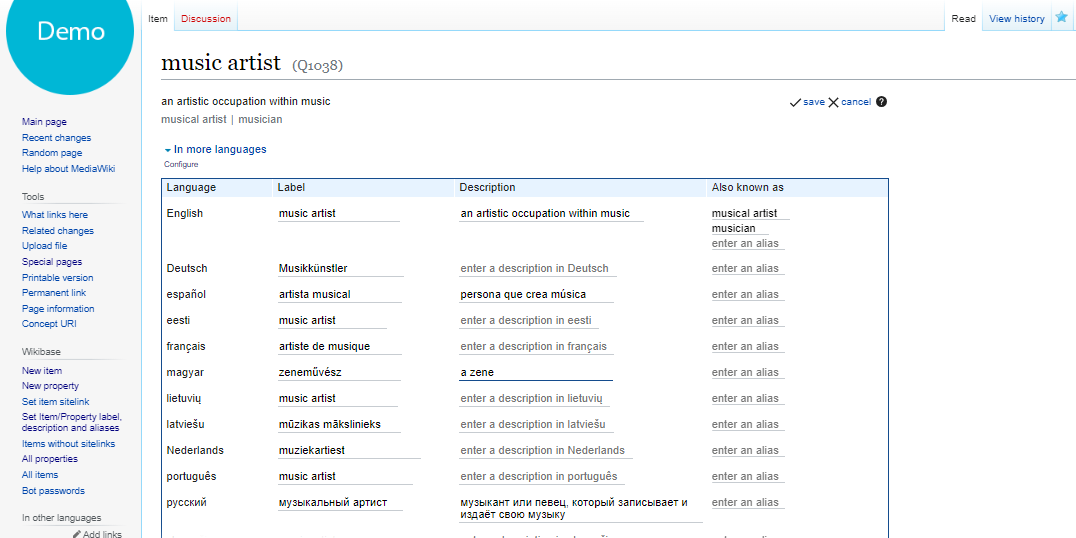
\includegraphics{png/wikibase/edit/add_new_translation_2x1.png}

\begin{tcolorbox}[enhanced jigsaw, opacityback=0, bottomrule=.15mm, rightrule=.15mm, toptitle=1mm, breakable, colbacktitle=quarto-callout-tip-color!10!white, colback=white, title=\textcolor{quarto-callout-tip-color}{\faLightbulb}\hspace{0.5em}{Tip}, leftrule=.75mm, toprule=.15mm, left=2mm, arc=.35mm, colframe=quarto-callout-tip-color-frame, coltitle=black, titlerule=0mm, bottomtitle=1mm, opacitybacktitle=0.6]

Wikidata, the world's biggest open knowledge graph uses the same
Wikibase software that we use. Editing entries on Wikidata is identical
to editing Wikibase. See Section~\ref{sec-first-edits-wikidata}.

\end{tcolorbox}

\subsection{Adding knowledge in
statements}\label{adding-knowledge-in-statements}

\section{Populating a Wikibase}\label{populating-a-wikibase}

Wikibase is an open knowledge base or universe when installed. We start
populating it with some \textbf{items}. In the Wikidata data model,
items are similar to things, and classes are also defined as items.

\begin{tcolorbox}[enhanced jigsaw, opacityback=0, bottomrule=.15mm, rightrule=.15mm, toptitle=1mm, breakable, colbacktitle=quarto-callout-note-color!10!white, colback=white, title=\textcolor{quarto-callout-note-color}{\faInfo}\hspace{0.5em}{Note}, leftrule=.75mm, toprule=.15mm, left=2mm, arc=.35mm, colframe=quarto-callout-note-color-frame, coltitle=black, titlerule=0mm, bottomtitle=1mm, opacitybacktitle=0.6]

A \emph{sandbox} instance is a Wikibase instance designated for
learning, testing, and experimenting. Reprex has created several sandbox
instances for onboarding our data curators and for educational purposes.
Please see Chapter~\ref{sec-reprex-sandbox} for getting an account on
such an instance.

\end{tcolorbox}

\subsection{Creating entities or
items}\label{creating-entities-or-items}

\begin{figure}[H]

{\centering 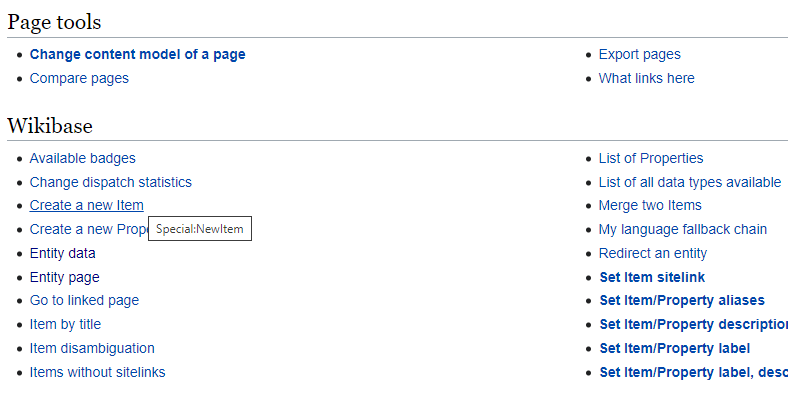
\includegraphics{png/wikibase/edit/create_new_item-1.png}

}

\caption{Special pages ➔ Wikibase ➔ Create a new item}

\end{figure}%%
\begin{figure}[H]

{\centering 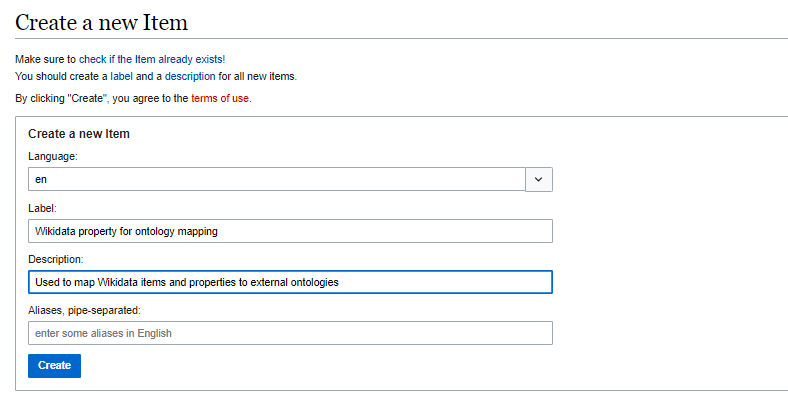
\includegraphics{png/wikibase/edit/create_new_item-2.png}

}

\caption{Identical to Wikidata: you must fill out at least the main
Label of the item, and a description. We use English (en) as the master
language for international cooperations.}

\end{figure}%

Suppose you want to make an item or property entity multi-lingual. In
that case, you must add at least a new label or description via the
Special Pages on the Graphical User Interface (i.e., using your
browser.) If you work with our import-export tool or the API, you can
set labels and descriptions in several languages in one command.

\begin{figure}[H]

{\centering 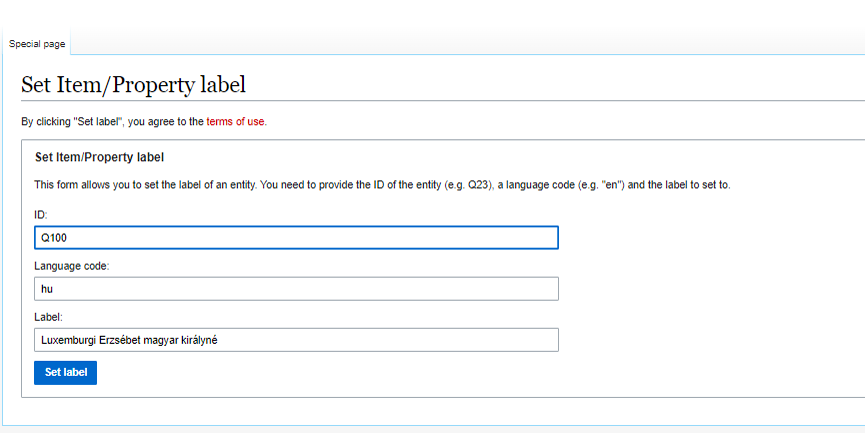
\includegraphics{png/wikibase/edit/add_new_language_label.png}

}

\caption{You can reach this form via the Special Pages ➔ Wikibase ➔ Set
Item/Property label or et Item/Description link.}

\end{figure}%

\subsection{Creating properties}\label{creating-properties}

Properties are describing relationships between items. You can create
them similarly to items, but navigating to Special pages ➔ Wikibase ➔
Create a new property (\emph{not item}). Properties are far more
important than items, because they define the rules of the knowledge
base. The type of relationships will allow our artificial intelligence
applications to make deductive or inductive new discoveries and expand
our knowledge.

In our introduction to Wikidata (Section~\ref{sec-wikidata}), you found
exactly the same graphical interface to work with items as on Wikibase,
but on the public Wikidata instance of Wikibase, you cannot find an add
new property button.

\begin{tcolorbox}[enhanced jigsaw, opacityback=0, bottomrule=.15mm, rightrule=.15mm, toptitle=1mm, breakable, colbacktitle=quarto-callout-note-color!10!white, colback=white, title=\textcolor{quarto-callout-note-color}{\faInfo}\hspace{0.5em}{Note}, leftrule=.75mm, toprule=.15mm, left=2mm, arc=.35mm, colframe=quarto-callout-note-color-frame, coltitle=black, titlerule=0mm, bottomtitle=1mm, opacitybacktitle=0.6]

On Wikidata, you are not allowed to create new properties: they are
created after a consultation with the Wikidata community. The addition
of properties determines who the knowledge graph will work in the
future.

\end{tcolorbox}

Needless to say that when you work with a Wikibase instance, you should
also be very careful with properties. While changing items usually
requires domain-specific knowledge, which you likely possess if you work
on an instance, the property sometimes requires knowledge about the
information or data model of the instance.

Not always: some properties are self-explanatory and very easy to create
and maintain. For example, the addition of identifiers to other data
systems is straightforward. Adding properties that define family
relationships (which have their logical rules) requires more careful
planning.

\begin{figure}[H]

{\centering 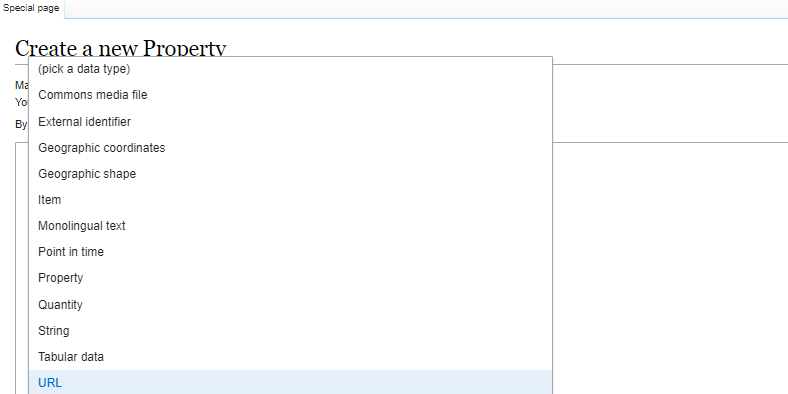
\includegraphics{png/wikibase/edit/create_new_property-2.png}

}

\caption{Properties have an extra field that you must fill out: the type
of expected data type.}

\end{figure}%

Properties have expected data types:

\begin{itemize}
\item
  Use a URL for connecting to other ontologies, data models (and add
  persistent URIs)
\item
  Use \emph{item} for entities that you want to weave together in the
  knowledge graph.
\item
  Use literal values like \emph{string} that for data that will be
  entered, but not will be placed on a graph.
\end{itemize}

For example, if you add \emph{Mai Manó} as a string, it will be
recorded, but you cannot connect with the works of Mai Manó, the
photographer. If you create an entity (item) for \texttt{Mai\ Manó}, you
will be able to link this entity to the works of Mai Manó, to his
children, to his house.

\subsection{Adding statements}\label{adding-statements}

Now we are ready to start to build an intelligent knowledge base. We
connect the \textbf{person} item in our Wikibase via the
\textbf{equivalent class} property to the
\href{https://www.cidoc-crm.org/html/cidoc_crm_v7.1.3.html\#E21}{E21\_Person}
definition of the CIDOC CRM. This will allow us to export our knowledge
base to a standard museological graph.

\begin{center}
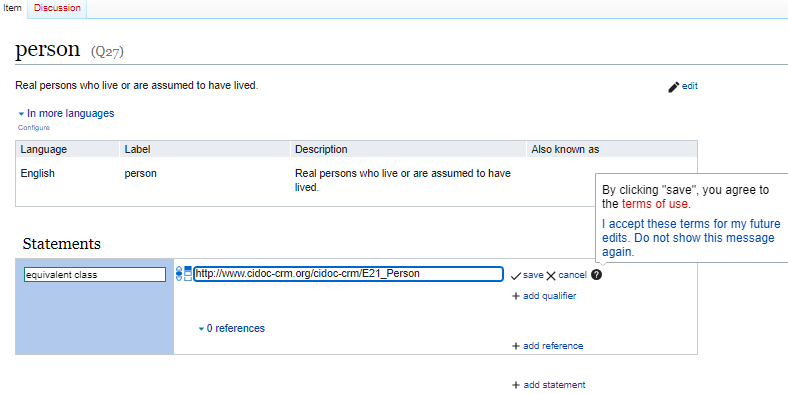
\includegraphics{png/wikibase/edit/add_new_statement-1.png}
\end{center}

In this case, the \texttt{equivalent\ class} property only accepts URLs.
The URI of the CIDOC definition of \texttt{E\_21\ Person} takes the
format of a URL so you can enter it here, but a simple string like E21
would not be allowed.

\begin{tcolorbox}[enhanced jigsaw, opacityback=0, bottomrule=.15mm, rightrule=.15mm, toptitle=1mm, breakable, colbacktitle=quarto-callout-note-color!10!white, colback=white, title=\textcolor{quarto-callout-note-color}{\faInfo}\hspace{0.5em}{Note}, leftrule=.75mm, toprule=.15mm, left=2mm, arc=.35mm, colframe=quarto-callout-note-color-frame, coltitle=black, titlerule=0mm, bottomtitle=1mm, opacitybacktitle=0.6]

Adding statements is exactly the same procedure on Wikibase as on
Wikidata (which is a gigantic Wikibase instance itself.) The only
difference is that you can only use properties (or items) that exist on
the Wikibase instance or Wikidata. Because Wikibase instances usually
should have a different knowledge coverage, some properties and items
are not available on others.

\end{tcolorbox}

\subsection{Synchronise with Wikidata}\label{synchronise-with-wikidata}

In our case, we want to be able to pre-fill data from Wikidata, and
then, eventually suggest changes in the public Wikidata. This requires
adding statements about Wikidata equivalent properties and items when
applicable.

\begin{figure}[H]

{\centering 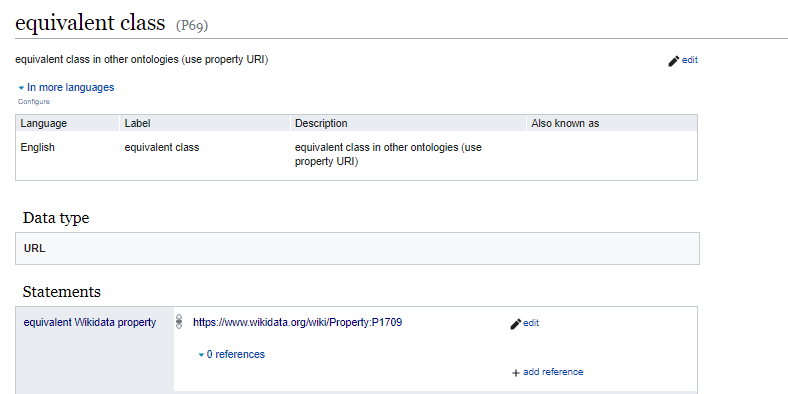
\includegraphics{png/wikibase/edit/data_fabric_property-1.png}

}

\caption{We created a special property, equivalent Wikidata property, to
link the P69 property definition in our Wikibase instance to Wikidata's
equivalent P1709. This will allow us synchronisation among the public
Wikidata and our Wikibase.}

\end{figure}%%
\begin{figure}[H]

{\centering 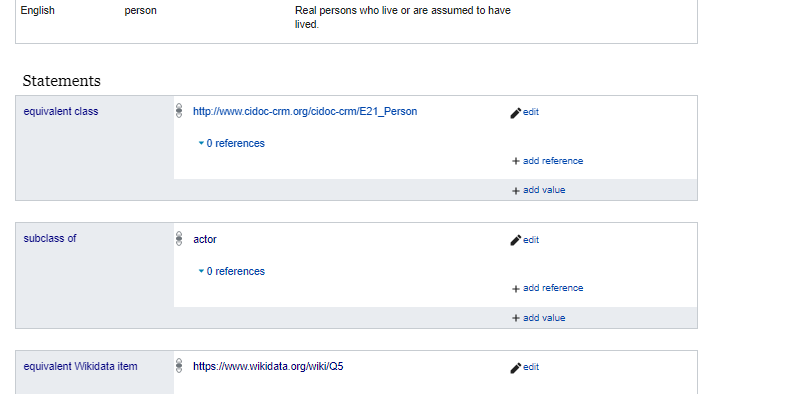
\includegraphics{png/wikibase/edit/data_fabric_entity-2.png}

}

\caption{For items (and classes are defined as items in Wikibase, just
like instances of persons), we created a special property equivalent
Wikidata item to keep the Person entity (see above its creation)
synchronised with Wikidata's Q5 item.}

\end{figure}%

Let us put this all together and create a bibliographic entry. Here we
will use a slight deviation from CIDOC, and use the
\href{https://www.wikidata.org/wiki/Property:P31}{instance of} property
(equivalently defined in our Wikibase with Wikidata) for class
inheritance. When we create a new entity (Manó Mai), we will define this
entity as an instance of a \texttt{person}. Persons have birth dates,
family members, they can create new creative works. In ontologies and in
RDF we call these abstract concepts classes.

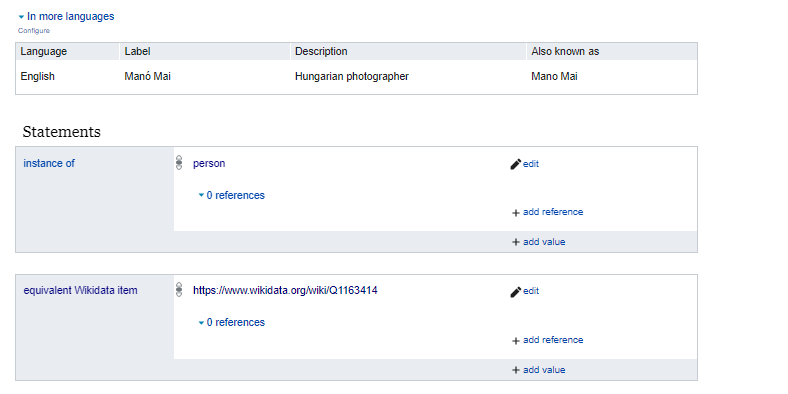
\includegraphics{png/wikibase/edit/create_new_item_mano-mai.png} We
immediately record that our entries about \emph{Manó Mai}, the great
photographer, should be talking about the same person as Wikidata's
\href{https://www.wikidata.org/wiki/Q1163414}{Q1163414} document item.

\section{Good practices}\label{good-practices}

Let us consider the creation of an entry for the Slovak composer,
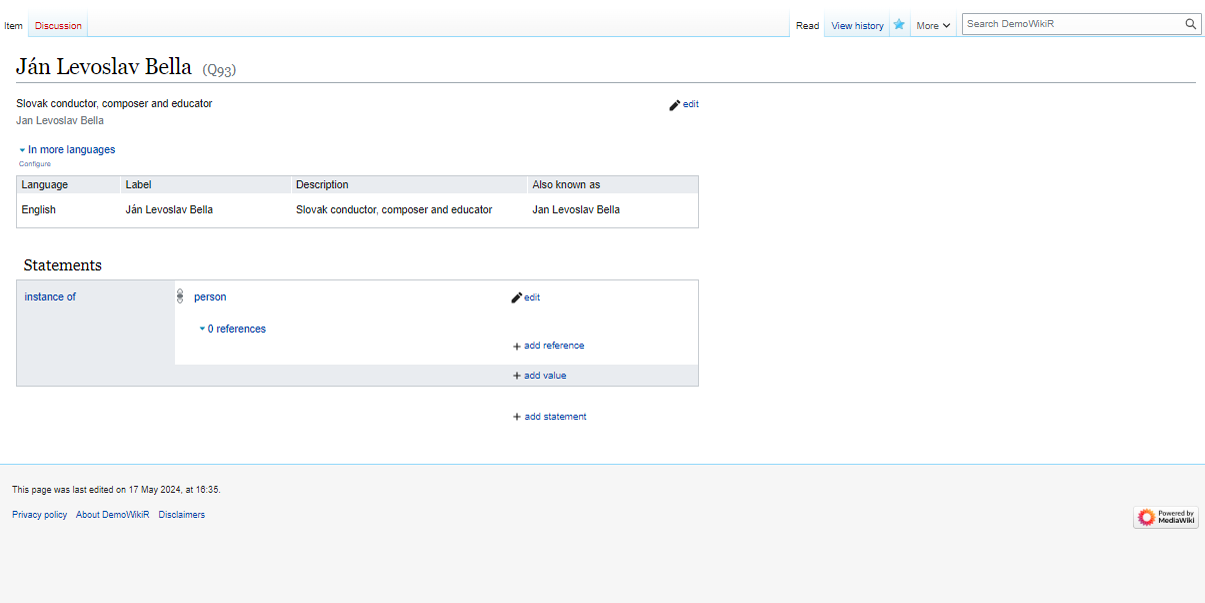
\includegraphics{png/wikibase/edit/bella/bella_1.png}

\subsection{Use of name strings or controlled
vocabularies}\label{use-of-name-strings-or-controlled-vocabularies}

In this case, we would like to code the \texttt{given\ name} property to
\texttt{Ján}. We can do it in two ways: - add the string \emph{Ján}
without further control, or, - add \texttt{Ján} as a controlled string
(an item \emph{datatype} on Wikibase.)

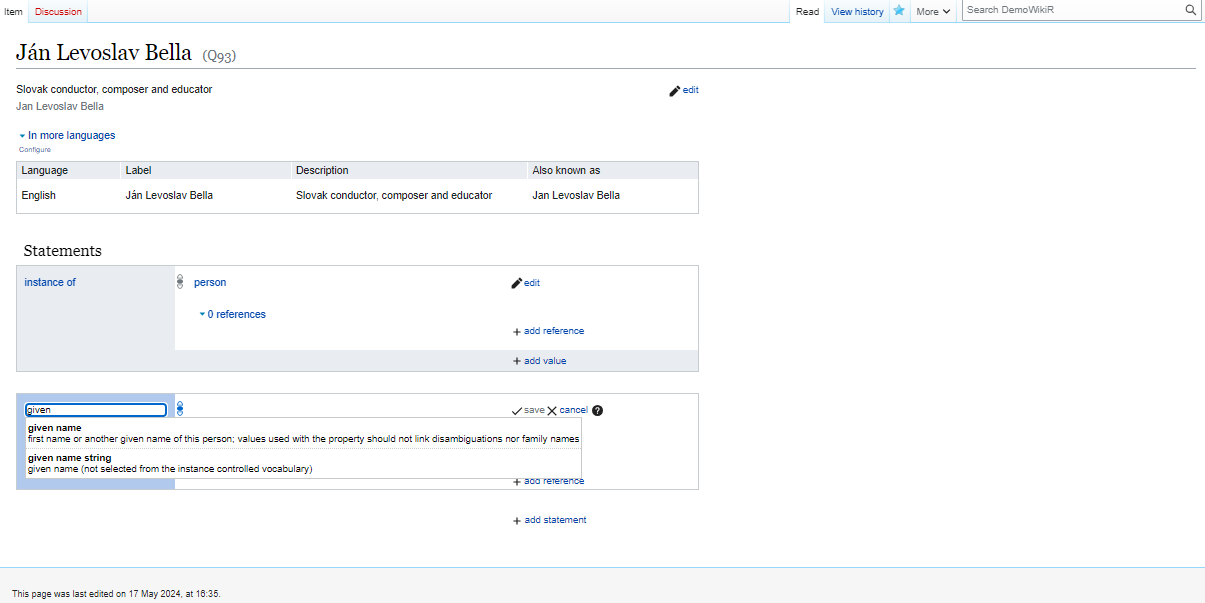
\includegraphics{png/wikibase/edit/bella/bella_2.png} Unless we can
import comprehensive datasets, usually data enrichment is a second step.
In such cases, we import first to a \texttt{name\ string} property given
names, locations, venue names, and other important nodes of our
knowledge graph.

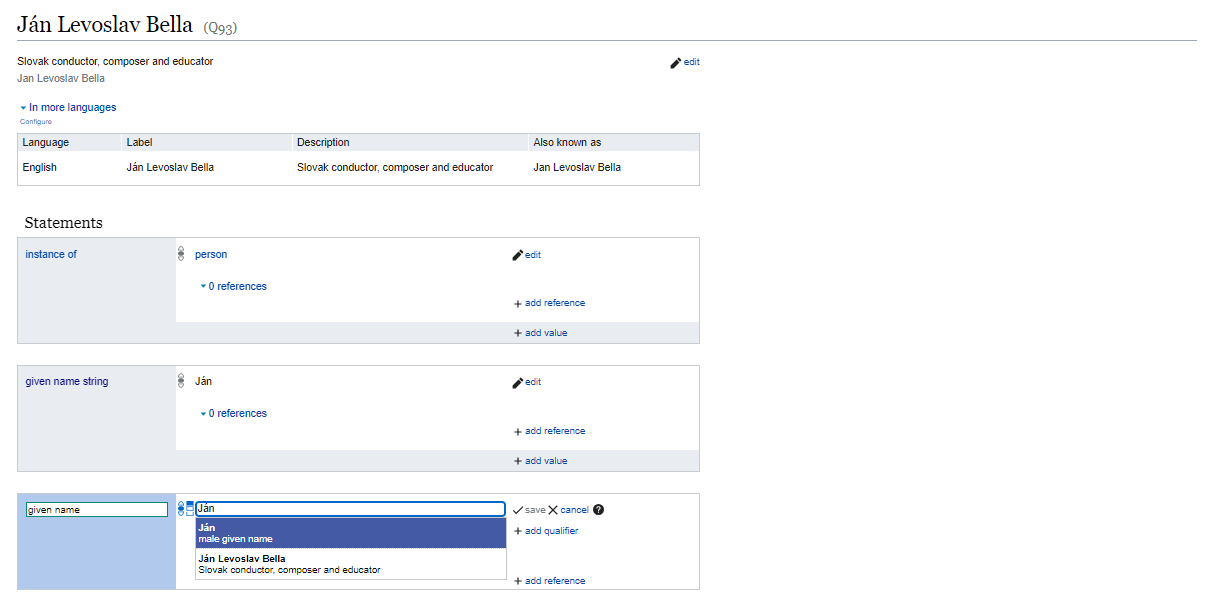
\includegraphics{png/wikibase/edit/bella/bella_3.png} The use of
controlled vocabularies makes filtering the database easier, and reduces
the likelihood of errorneous entries. In the Wikidata data model, we can
add a taxonomical class to such controlled vocabulary items. By coding
\texttt{Ján} as an instance of the \texttt{Slovak\ make\ given\ name},
we can later search composers or persons easer by this name given name
or we can infer that the composer was born as a man.

\begin{figure}[H]

{\centering 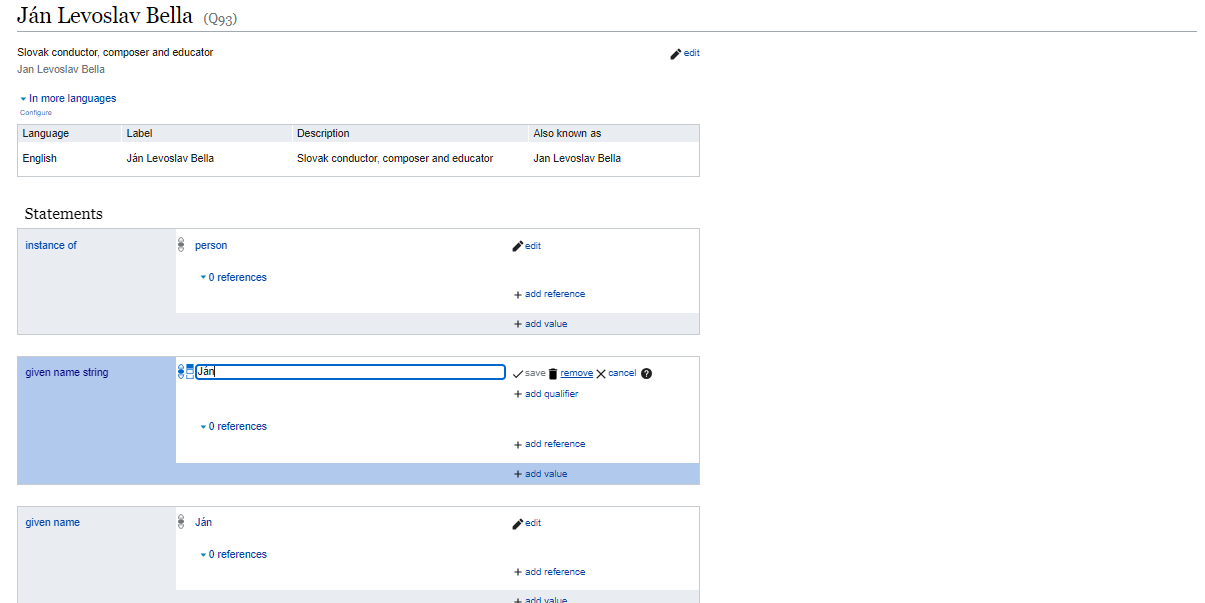
\includegraphics{png/wikibase/edit/bella/bella_4.png}

}

\caption{The use of controlled vocabularies (and items) have many
advantages.}

\end{figure}%

In this case, we would like to code the \texttt{given\ name} property to
\texttt{Ján}. We can do it in two ways: add \texttt{Ján} as a controlled
string (an item \emph{datatype} on Wikibase) and add the string
\emph{Ján} without further control.

Coding \texttt{Ján}. to Ján must be done with the knowledge of the data
curator. We can only make this coding if we know that the string
\emph{Ján} came from a \texttt{given\ name} (or equivalent) database
table column, if indeed it comes from a database of Slovak persons. This
is one of the reasons why our \texttt{bots}, i.e., automated importing
tools will map given names first to the \texttt{given\ name\ string}
property.

\textbf{Similar name string properties:}

\begin{itemize}
\item[$\square$]
  \texttt{location\ of\ first\ performance\ (string)},
  \texttt{location\ of\ creation\ (string)}: The strings
  \texttt{Bratislava}, \texttt{Bratislava,\ CS},
  \texttt{Bratislava,\ SK}, \texttt{Bratislava,\ Austria-Hungary} or map
  to the \texttt{item:Bratislava}.
\item[$\boxtimes$]
  \texttt{location\ of\ first\ performance},
  \texttt{location\ of\ creation}: locations must be items of the class
  \texttt{city}, \texttt{town}, \texttt{village} (they all have their
  regional and country entities), or \texttt{region} (they have their
  country) or \texttt{country}. The city item
  \href{https://www.wikidata.org/wiki/Q1780}{Bratislava} contains the
  knowledge that this is the current capital city of the Slovak
  Republic, and it is a former town in Czechoslovakia and
  Austria-Hungary (it has 232 statements which enrich the concept of
  \texttt{Bratislava}), and it is connected to lists like
  \href{https://en.wikipedia.org/wiki/List_of_people_from_Bratislava}{List
  of people from Bratislava}.
\item[$\square$]
  \texttt{venue\ of\ first\ performance\ (string)}: the string
  \emph{Jesuit Church of St.~Francis Xavier} will need to be matched to
  a venue item
\item[$\boxtimes$]
  \texttt{venue\ of\ first\ performance}:
  \href{https://reprexbase.eu/demowiki/index.php?title=Item:Q94}{Jesuit
  Church of St.~Francis Xavier, Skalica, Slovakia} as a venue item,
  which can be a class of building, or an atelier, or a concert hall
  within a building.
\item[$\square$]
  \texttt{event\ of\ the\ first\ performance\ (string)}:
  \texttt{Prague\ Spring\ International\ Music\ Festival}---this is not
  a venue but a festival event.
\item
  \texttt{event\ of\ the\ first\ performance}:
  \href{https://www.wikidata.org/wiki/Q1776937}{Prague Spring
  International Music Festival} is a repeating event, and it has its own
  entity among music festivals.
\end{itemize}

\section{The EU Knowledge Graph}\label{sec-eu-knowledge-graph}

\begin{figure}[H]

{\centering 
\includegraphics{png/wikibase/EU-academy-course/EU-knowledge-graph.png}

}

\caption{EU Academy Course: EU Knwoledge Graph}

\end{figure}%

Because of the success of Wikidata, many projects and institutions are
looking into Wikibase, the software that runs Wikidata. They aim to
reuse the software to construct institutional or cross-institutional,
domain-specific knowledge graphs. Several factors make Wikibase
attractive:

\begin{itemize}
\item[$\boxtimes$]
  the fact that it is a well-maintained open-source software;
\item[$\boxtimes$]
  there is a rich ecosystem of users and tools around it;
\item[$\boxtimes$]
  \href{https://www.wikimedia.de/}{Wikimedia Deutschland↗} (WMDE), the
  maintainer of Wikibase, has made considerable investments in
  optimising the software's use outside of Wikidata or other Wikimedia
  projects;
\item[$\boxtimes$]
  The \href{https://linkedopendata.eu/wiki/The_EU_Knowledge_Graph}{EU
  Knowledge Graph↗} runs on Wikibase;
\item[$\boxtimes$]
  The \emph{EU Academy} and the \emph{EU Open Data Portal} actively
  disseminate good practices and know-how on its implementation in
  cross-institutional data-sharing programs.
\end{itemize}

Our OpenCollections instances are prepared with a similar mindset to the
creation of the
\href{https://linkedopendata.eu/wiki/The_EU_Knowledge_Graph}{EU
Knowledge Graph↗}. We pre-populate a Wikibase instance from Wikidata
about many institutional, geographical or biographical facts of the
domain (Diefenbach, Wilde, and Alipio 2021), or with elements of the
Wikidata data model and its compatibility classes with other ontologies.

\section{EU Academy Course on
Wikibase}\label{eu-academy-course-on-wikibase}

\begin{figure}[H]

{\centering 
\includegraphics{png/wikibase/EU-academy-course/eu_academy_course.png}

}

\caption{The EU Academy course on using Wikibase and Semantic MediaWiki}

\end{figure}%

\textbf{Target audience}

Policymakers, public administrators, data maintainers, IT professionals.

\textbf{Learning objectives}

\begin{itemize}
\item
  Pros and cons of using Wikibase/SMW for your dataspace
\item
  Lessons learnt from projects already using Wikibase/SMW instances
\item
  Practical know-how about setting up a new Wikibase/SMW from scratch
\item
  What should be on Wikidata vs in a local Wikibase/SMW
\item
  Comparison between Wikibase and SMW
\end{itemize}

\textbf{Offered by}

This content is offered by the European Commission. The European
Commission is the European Union's politically independent executive
arm. It is alone responsible for drawing up proposals for new European
legislation, and it implements the decisions of the European Parliament
and the Council of the European Union.

\bookmarksetup{startatroot}

\chapter{Reprex's Sandbox}\label{sec-reprex-sandbox}

\section{Create an Account}\label{sec-opencollections-create-account}

Depending on the type of MediaWiki+Wikibase instance you are using, you
may need to create an account to access the site. The process may be
less or more strict, depending on how much private data the instance
holds.

\begin{enumerate}
\def\labelenumi{\arabic{enumi}.}
\item
  Access
  \href{https://reprexbase.eu/sandbox/index.php?title=Main_Page}{Reprex's
  Sandbox Environment.} Beware, we have multiple instances, so
  \emph{access the instance with its URL where you have an invitation}.
\item
  On this page, select \textbf{Request Account}.
\end{enumerate}

\begin{figure}[H]

{\centering 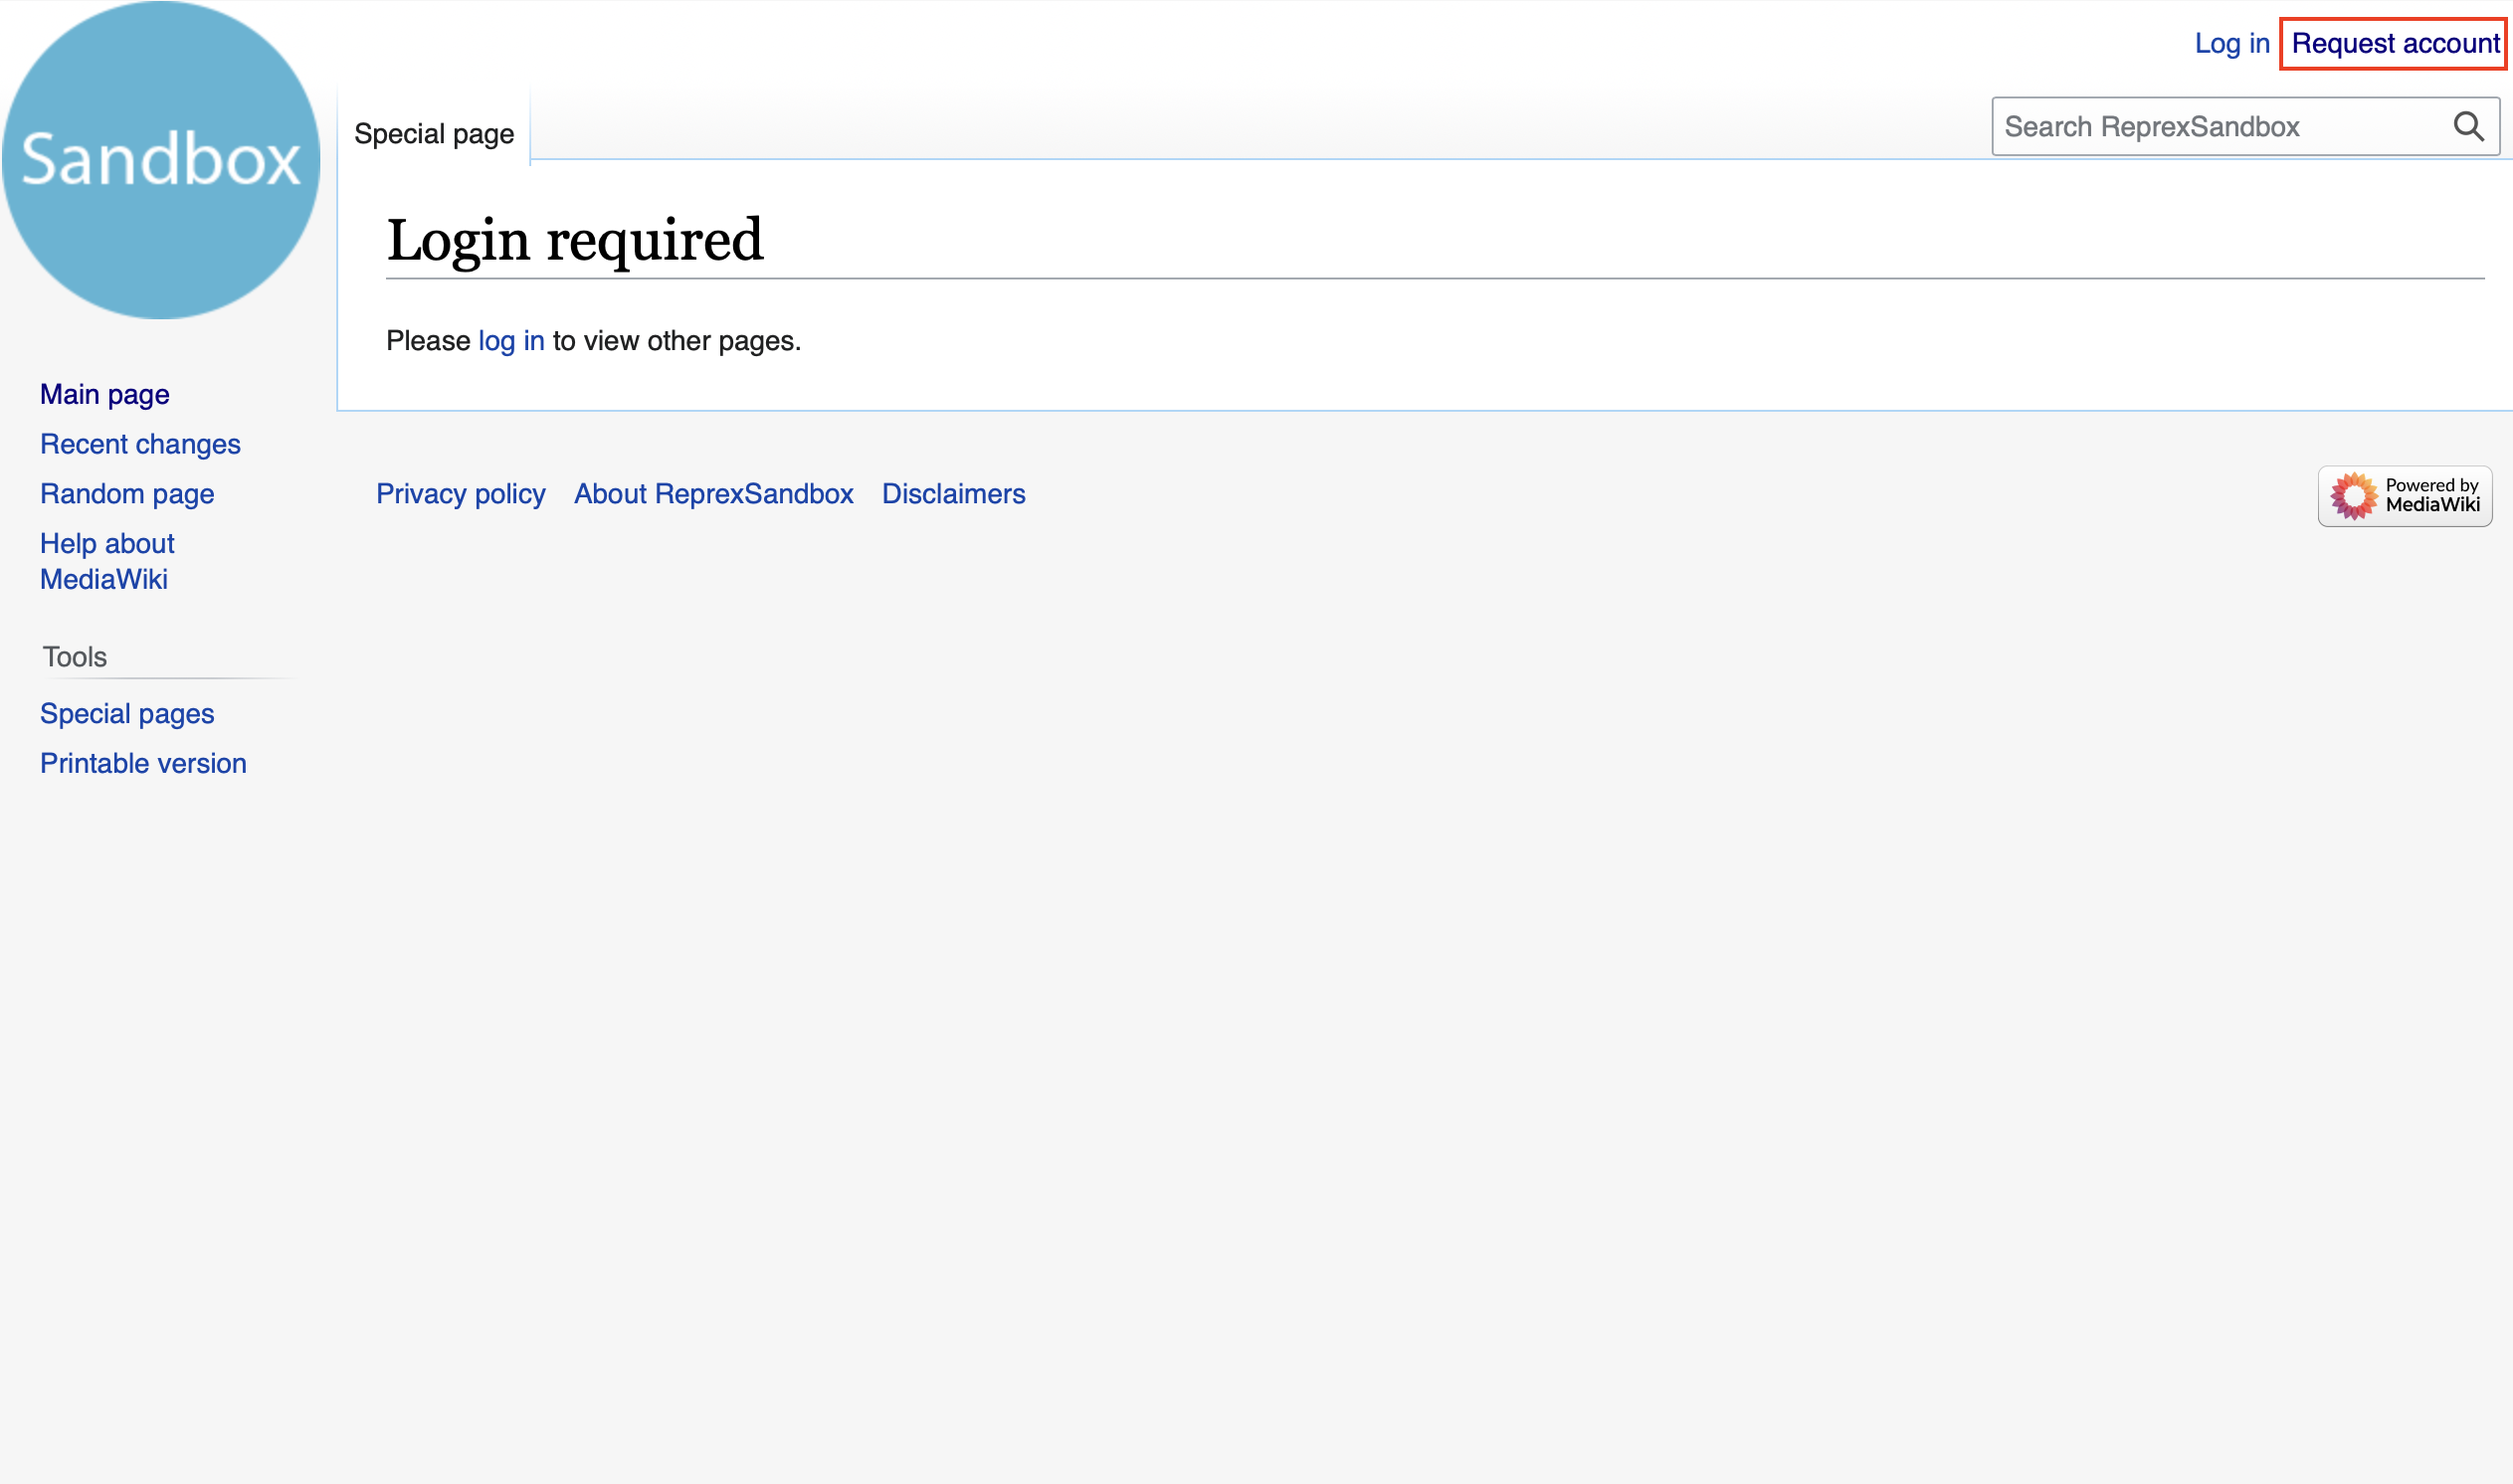
\includegraphics{png/wikibase/request-account_1.png}

}

\caption{Request account - beware, we maintain several sandbox and live
production instances, you must navigate to the one wher eyou really want
to have this account.}

\end{figure}%

\begin{enumerate}
\def\labelenumi{\arabic{enumi}.}
\setcounter{enumi}{2}
\tightlist
\item
  On the next page, type in your chosen \textbf{username} and your
  \textbf{email address}. For a username, use a professional one that is
  similar to what you use on Keybase, Github, etc. Then confirm by
  clicking \textbf{request account} again.
\end{enumerate}

\begin{figure}[H]

{\centering 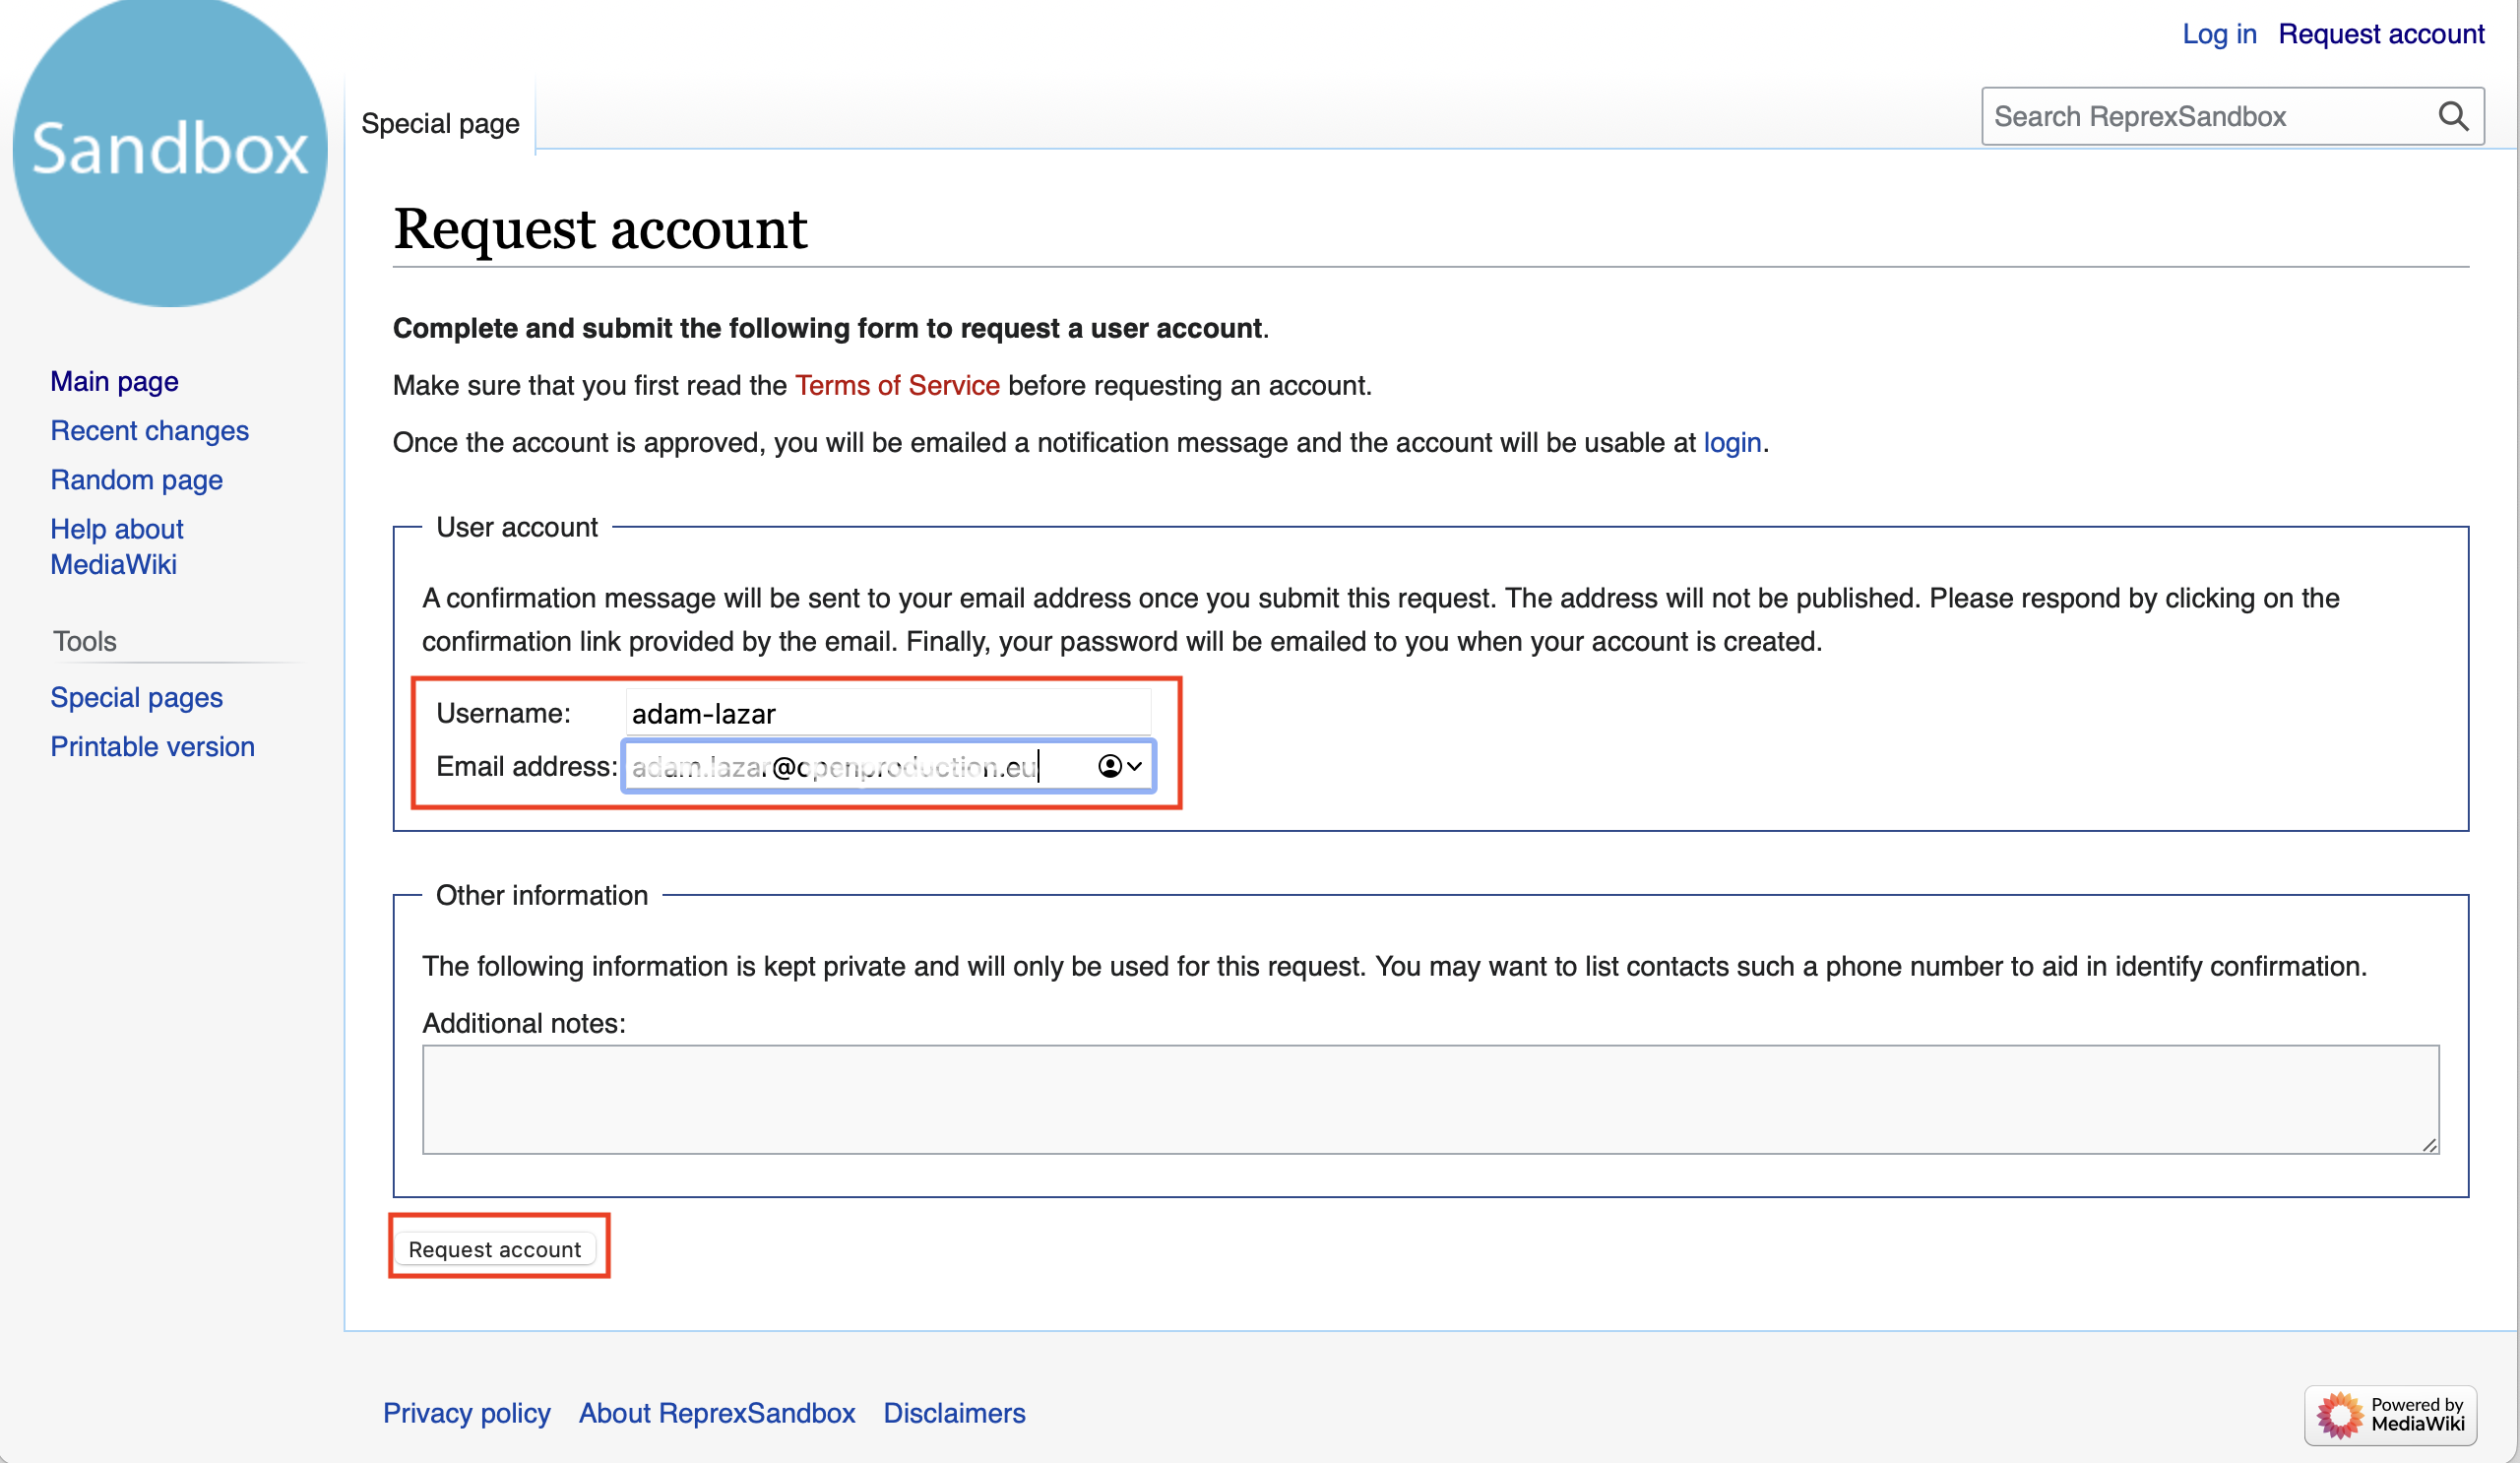
\includegraphics{png/wikibase/request-account_2.png}

}

\caption{Usernames on Wikibase always start wih a capital letter, i.e.,
Janedoe, or Jane.doe, Or Jane.Doe.}

\end{figure}%

\begin{enumerate}
\def\labelenumi{\arabic{enumi}.}
\setcounter{enumi}{3}
\tightlist
\item
  Check your email inbox now. You should receive an email with a
  confirmation link. Click on this confirmation link. (The
  machine-generated email may easily go to the spam box.)
\end{enumerate}

\begin{figure}[H]

{\centering 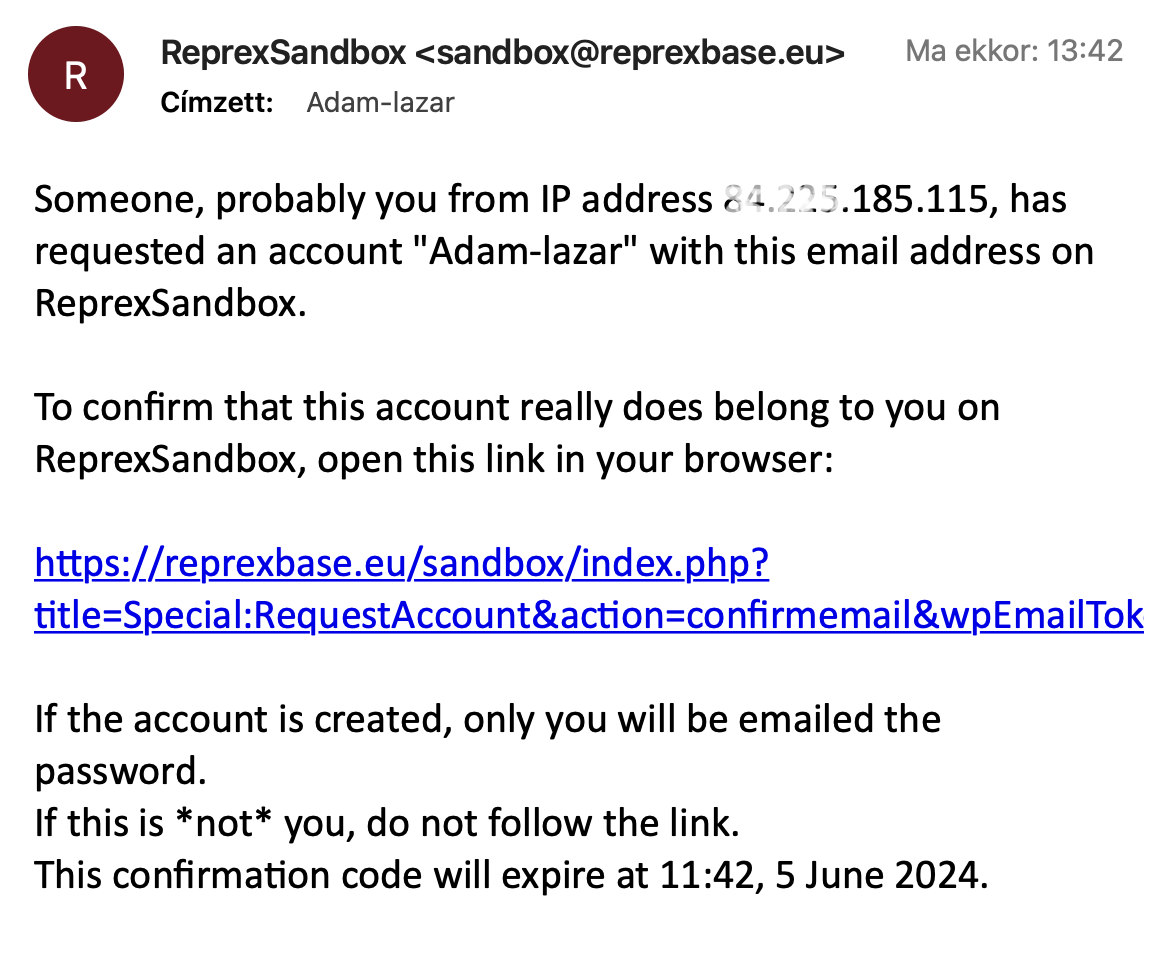
\includegraphics{png/wikibase/request-account_confirmation-email.png}

}

\caption{Often the confirmation mail ends up in your spam.}

\end{figure}%

\begin{enumerate}
\def\labelenumi{\arabic{enumi}.}
\setcounter{enumi}{4}
\tightlist
\item
  After you confirm your account request, the administrators of the
  Wikibase instance will evaluate it. Then, you will receive another
  email with your login credentials, including your temporary password.
\end{enumerate}

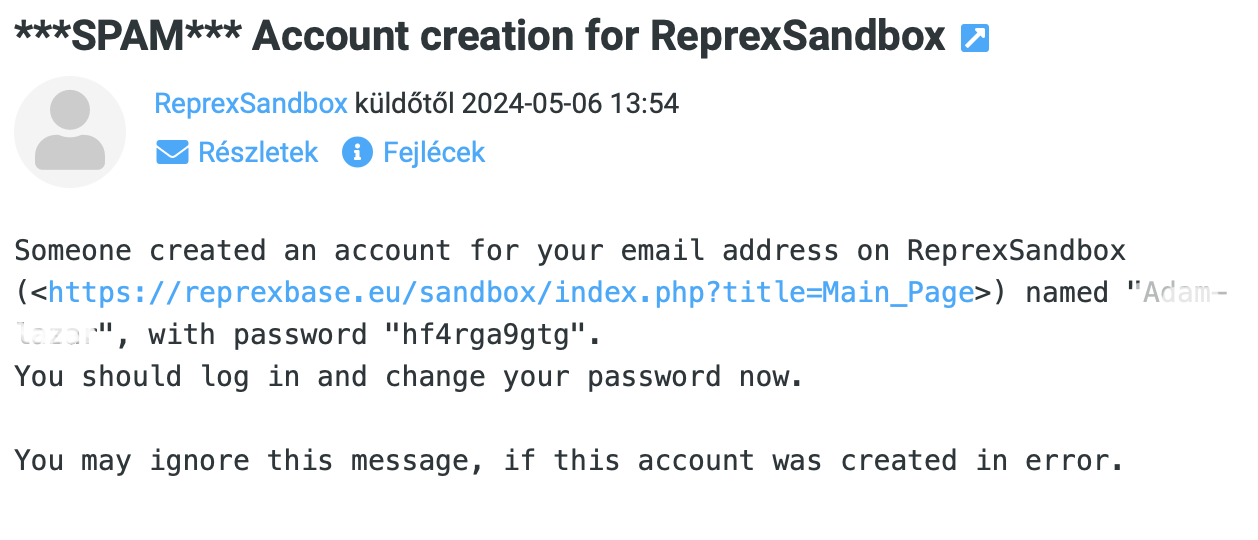
\includegraphics{png/wikibase/request-account_email-with-temporary-login-credentials.png}

\begin{enumerate}
\def\labelenumi{\arabic{enumi}.}
\setcounter{enumi}{5}
\tightlist
\item
  Revisit the sandbox page and log in. On the login page, type your
  username and the temporary password you received, then click
  \textbf{Log In}. You will be automatically taken to the next page,
  where you must change your password by typing your new permanent
  password. Provide your new password, then confirm it.
\end{enumerate}

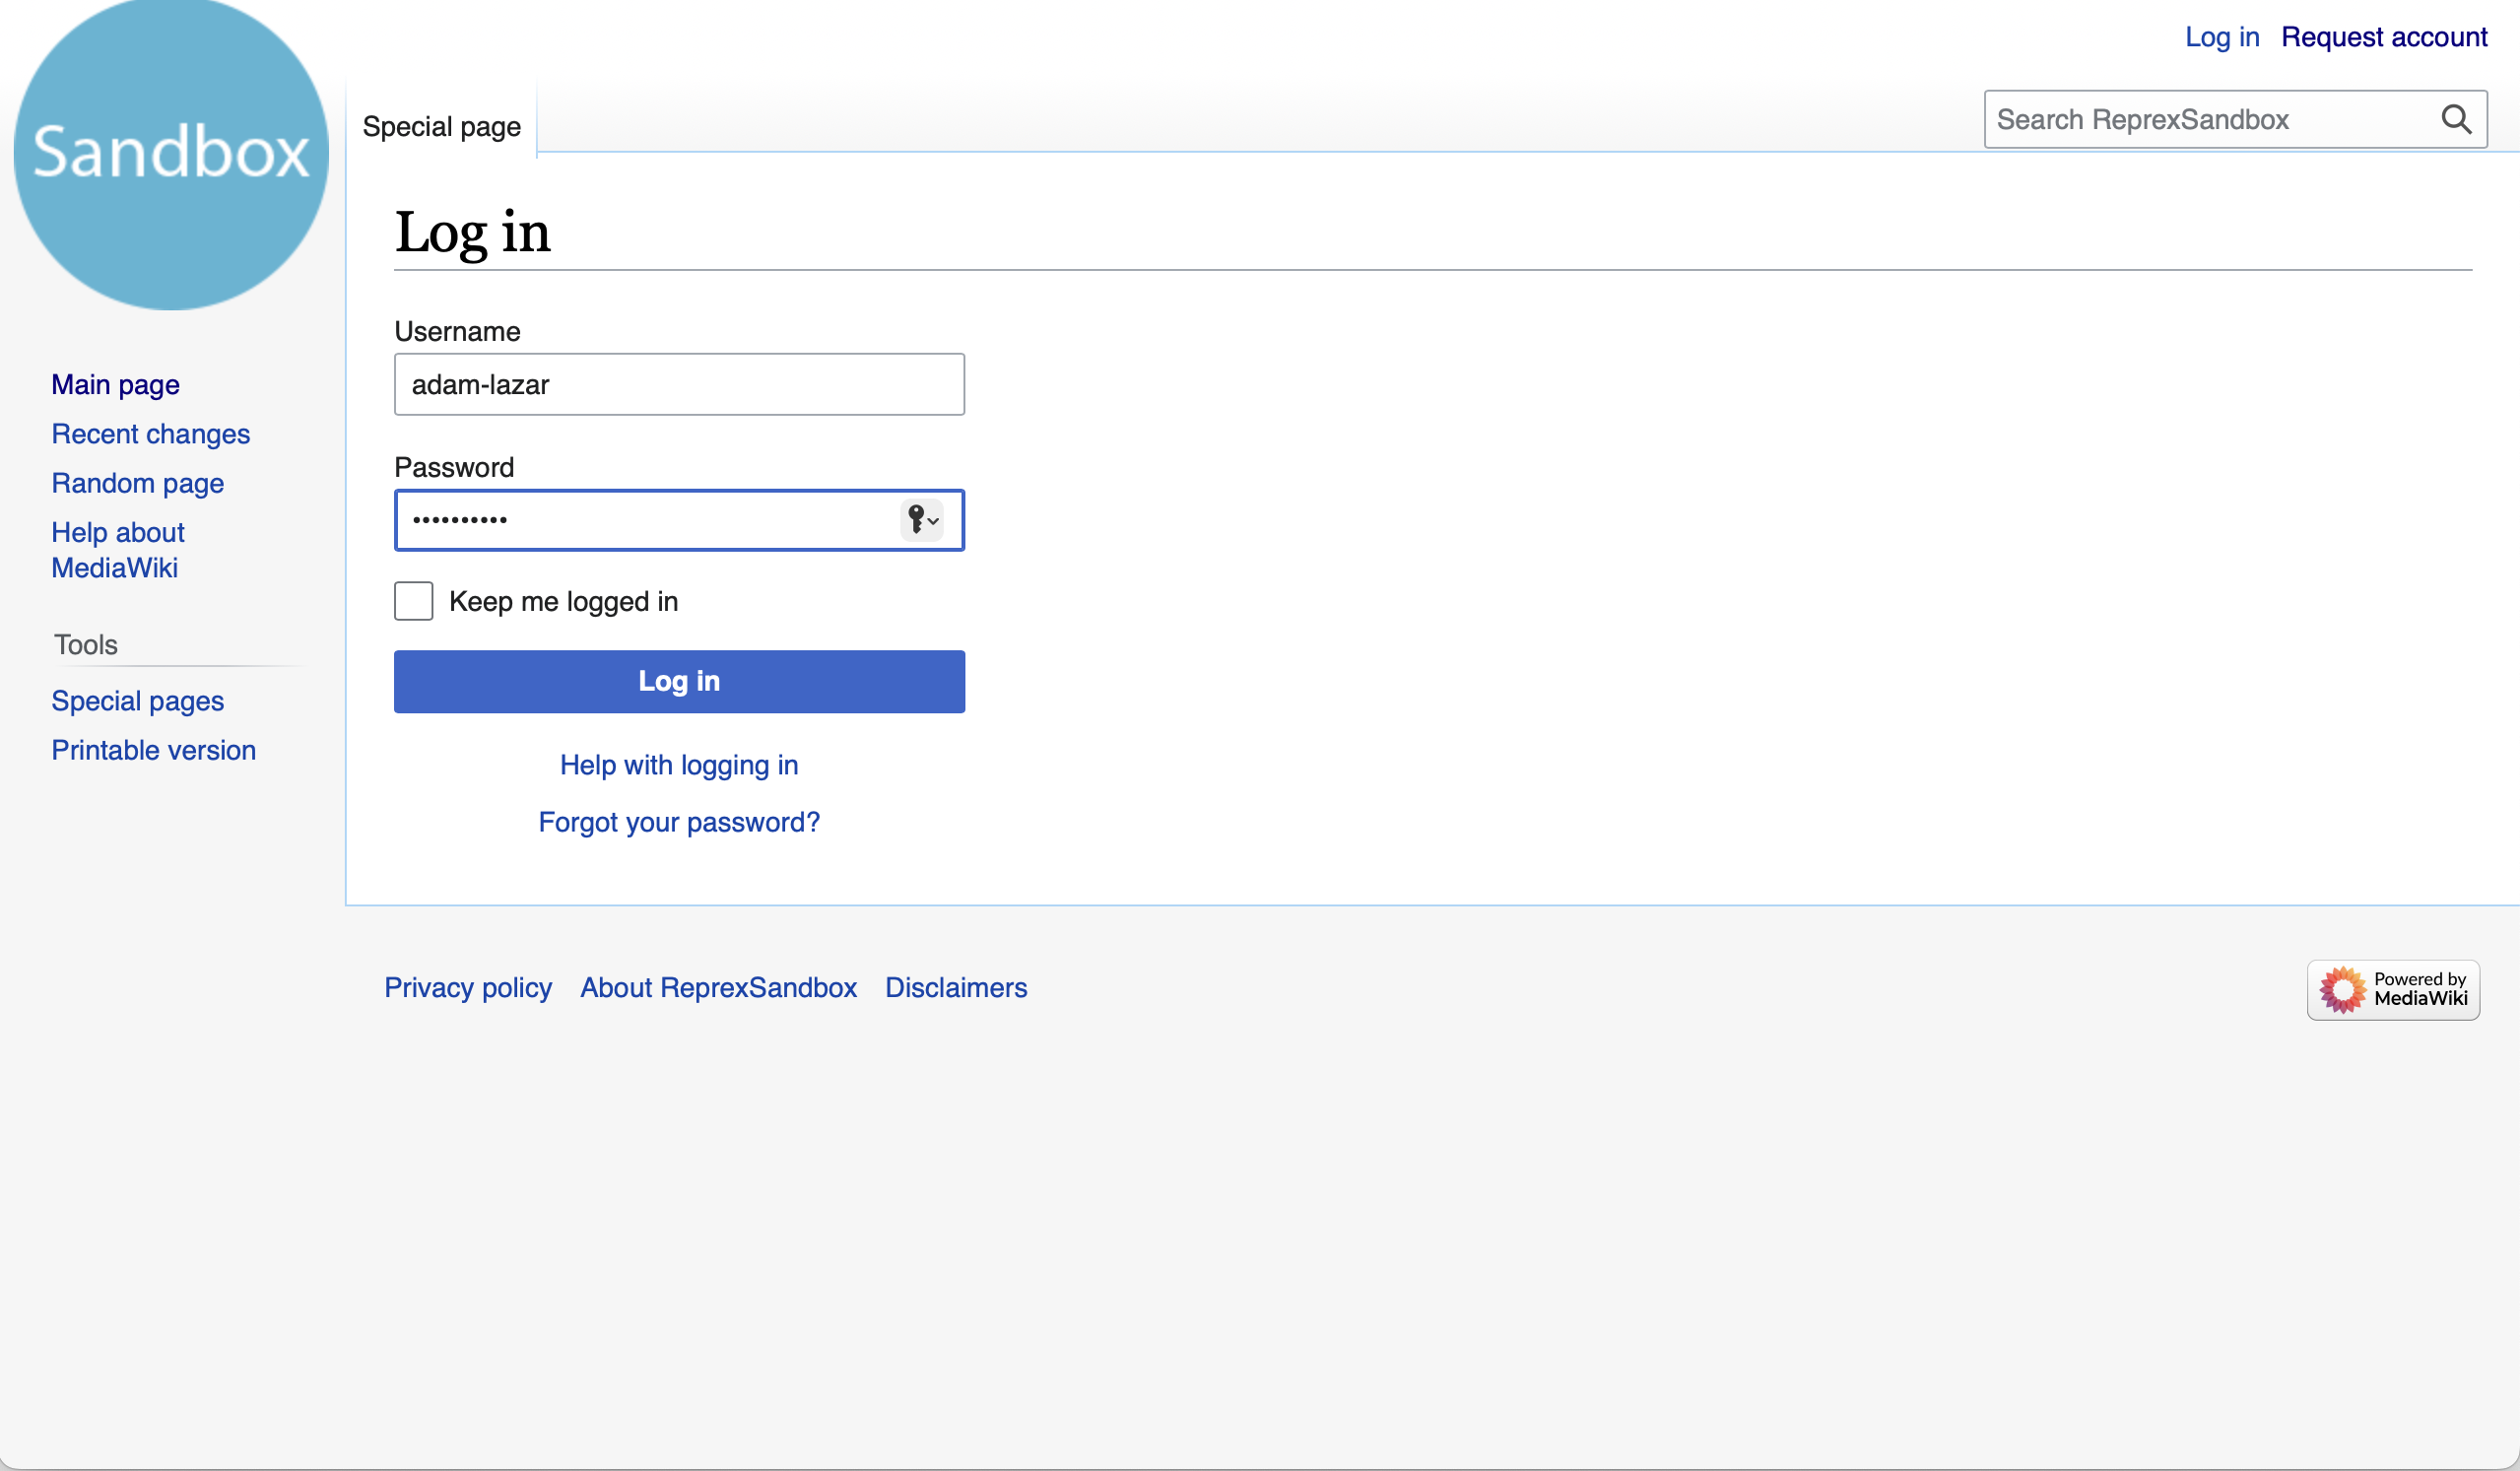
\includegraphics{png/wikibase/request-account_log-in-page.png}

\begin{enumerate}
\def\labelenumi{\arabic{enumi}.}
\setcounter{enumi}{6}
\tightlist
\item
  All done; you are now logged in to your account.
\end{enumerate}

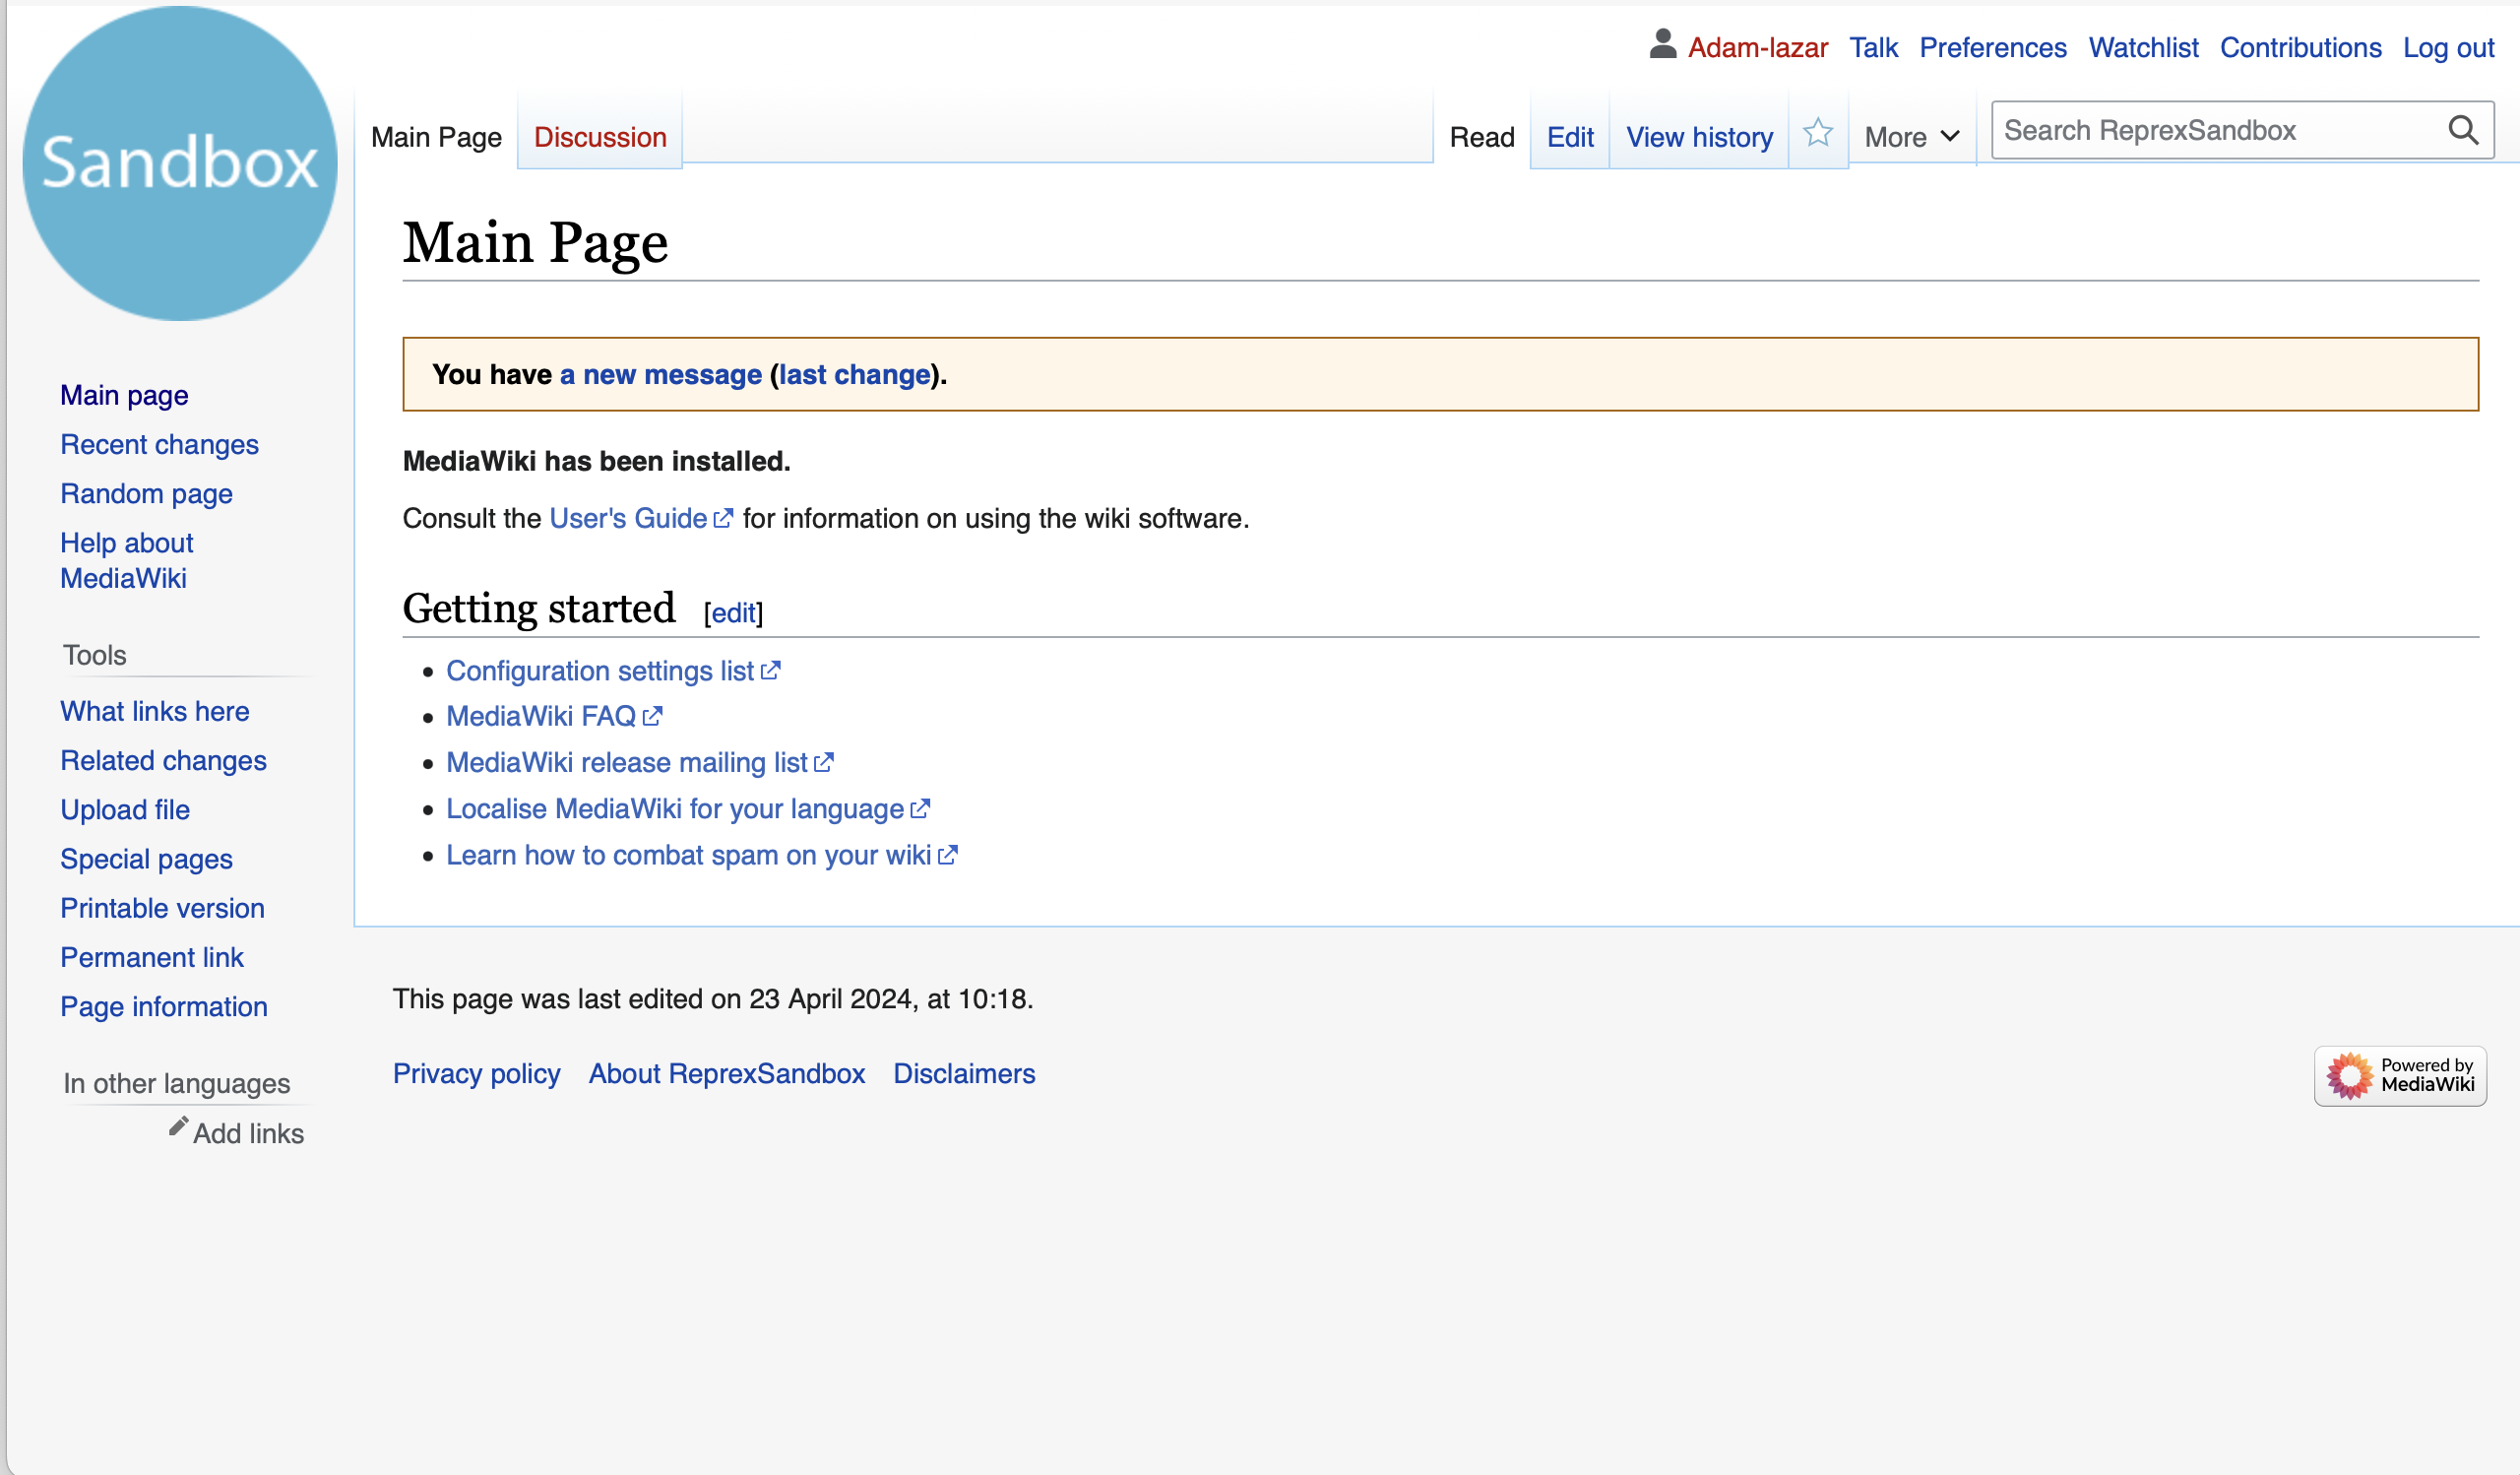
\includegraphics{png/wikibase/request-account_logged-in.png}

\section{Editing data}\label{editing-data}

\section{Weaving Data Into the Knowledge
Graph}\label{weaving-data-into-the-knowledge-graph}

Just because we edit data in a Wikibase instance, it will not
necessarily be more usable than a spreadsheet or a simple local
database. If we add \texttt{42} without a context, such as age or the
number of tracks, these two numeric characters will be only literal
numbers. We can increase knowledge by making every point of information
a node in the knowledge graph, an edge where new information can flow
in.

In Wikibase, we call these nodes entities. If we make Albert Einstein an
entity instead of the string Albert Einstein, we will be able connect
knowledge about his life, his scientific work, proofs, photographs of
his lectures, and other forms of knowledge.

When we start importing information into a knowledge graph or begin
editing and enriching information within the graph, we are faced with a
crucial decision. We must determine which data points, such as cells in
an original spreadsheet, or database table, or financial ledger, should
be elevated to the status of nodes in the graph. These nodes, or
entities, have the potential to develop their own relationships, thereby
enriching the overall knowledge graph. Understanding this
decision-making process empowers us to effectively utilize Wikibase for
our data management needs.

\subsection{Improving relational
databases}\label{improving-relational-databases}

When the aim is to improve the data quality, content, or timeliness of a
relational database system, the first and most essential candidates to
become entities are the database's primary and secondary keys. To recall
our simple example from Section~\ref{sec-wikidata},

\begin{longtable}[]{@{}
  >{\raggedright\arraybackslash}p{(\columnwidth - 4\tabcolsep) * \real{0.2361}}
  >{\raggedright\arraybackslash}p{(\columnwidth - 4\tabcolsep) * \real{0.3194}}
  >{\raggedright\arraybackslash}p{(\columnwidth - 4\tabcolsep) * \real{0.4444}}@{}}
\toprule\noalign{}
\begin{minipage}[b]{\linewidth}\raggedright
ID
\end{minipage} & \begin{minipage}[b]{\linewidth}\raggedright
Author
\end{minipage} & \begin{minipage}[b]{\linewidth}\raggedright
Title
\end{minipage} \\
\midrule\noalign{}
\endhead
\bottomrule\noalign{}
\endlastfoot
My-01 & Martell, Yann
(\href{https://www.wikidata.org/wiki/Q13914}{Q13914}) & \emph{Life of
Pi} (\href{https://www.wikidata.org/wiki/Q374204}{Q374204}) \\
\ldots{} & \ldots{} & \ldots{} \\
My-42 & Adams, Douglas (\href{https://www.wikidata.org/wiki/Q42}{Q42}) &
\emph{Hitchhiker's Guide to the Galaxy}
\href{https://www.wikidata.org/wiki/Q25169}{Q25169}) \\
\ldots{} & \ldots{} & \ldots{} \\
\end{longtable}

\begin{quote}
If you can connect your My-42 entry with
\href{https://www.wikidata.org/wiki/Q25169}{Q25169} on Wikidata, you can
import a wealth of information into your private catalogue. And if you
add \href{https://www.wikidata.org/wiki/Q42}{Q42} to the author Douglas
Adams, you can import a lot of knowledge, for example, information about
his other works or the end of the copyright protection term of these
books, after which they will become public domain and free for copying
and distribution.
\end{quote}

Intuitively, in Wikibase, this means that we ``conceptualise'' authors
and their books. The person known as \emph{Douglas Adams} becomes a
human, a creator, and a writer, with all the properties that writers
have\ldots{} such as books. The \emph{Hitchhiker's Guide to the Galaxy}
will turn from string into the concept of a \texttt{Book}. As soon as we
state that this is a book, not merely a text, we can start adding
book-specific knowledge to the
\texttt{Hitchhiker\textquotesingle{}s\ Guide\ to\ the\ Galaxy} book
entity: ISBN number, first publication date, translations. And what is
most important, we can connect this entity with the author,
\texttt{Douglas\ Adams}, who is no longer just one of the many people
who are known by this name, but the person who wrote quiet humorous
books.

Conceptualisation is possibly manually, as we have shown in
Section~\ref{sec-wikidata}; but usually we do this after data modelling
with bulk importing. You tells us what is your data about: books and
author, and we import them as \texttt{Books} and \texttt{Authors}, so
that we can start to look for more information about these books and
authors in various knowledge systems.

\subsection{Improving spreadsheet
databases}\label{improving-spreadsheet-databases}

Smaller organisations often do not use relational databases; instead,
they use Excel or OpenOffice spreadsheets maintained by workers, often
for decades. Turning such spreadsheets into knowledge base elements is
similar to working with a relational database, but sometimes, it is a
smaller and more difficult task.

Well-organised spreadsheets can be good databases because spreadsheet
applications like Excel, OpenOffice, or Google Spreadsheet allow the use
of primary and secondary keys by connecting worksheets and the creation
of pivot tables.

The key challenge with spreadsheets is identifying the Things that
should become entities. What is your spreadsheet about? Buildings? Then,
addresses and building names should become entities and nodes in the
graph. Addresses keep changing, building geometries keep changing, and
new additions are built or demolished. Street names change. Even city
names change; cities merge and divide.

\subsection{Improving annotated text, legal documents, lab notes,
regulatory
filings}\label{improving-annotated-text-legal-documents-lab-notes-regulatory-filings}

\subsection{Creating new indicators}\label{creating-new-indicators}

\bookmarksetup{startatroot}

\chapter{Bulk import}\label{bulk-import}

\section{Organise your data}\label{organise-your-data}

In the Chapter~\ref{sec-tidy} chapter on tidy data we have shown one of
the advantages of a tidy dataset: it can be pivoted into a sequence of
triple-form semantic statements. This is possible because tidy format is
unambiguous: we always know that a number or string (value) belongs to
its observational subject (in the rows) and the measured property
variable (in the columns). In other words, the meaning of a cell is
unambiguous, because we know the subject (from the rows) and the
predicate (from the column headings.)

\begin{center}
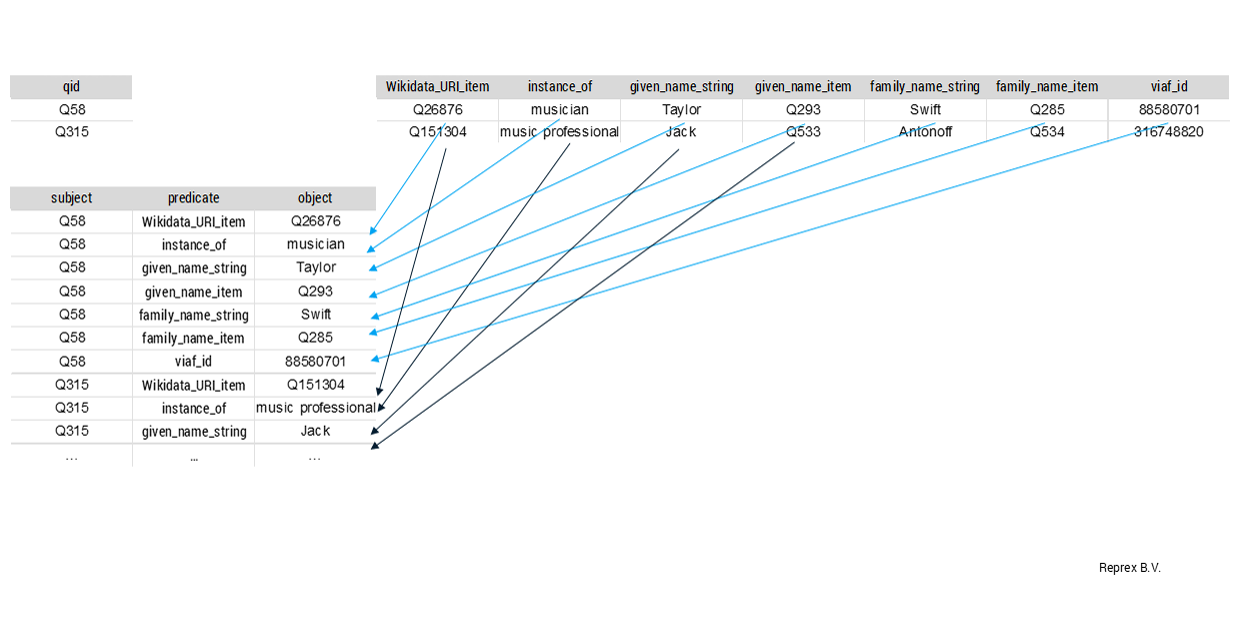
\includegraphics{png/tidy/pivot_longer_to_statements_notitle_2x1.png}
\end{center}

In the Chapter~\ref{sec-collections} chapter we have seen that naming is
hard. Weather we are talking about people, objects, or table variables,
it is difficult to come up with good names. Most programmers and
open-source communities apply variable naming conventions.

We apply the \texttt{snake\ case} convention, which creates variables
like \texttt{given\_name\_string}. We make these names tidier with
grouping semantic elements into the beginning or ending of the variable
name; this way the variable name can be filtered easily.

When importing into Wikibase, we need to know what should be the
\texttt{type} of the imported data. Shall we use a string for
\texttt{Taylor} and \texttt{Swift}, or we want to create an entity for
the name (variants) of \texttt{Taylor}?

\begin{itemize}
\item[$\boxtimes$]
  The Q number (\texttt{QID}) is unique to each Wikibase, including your
  Wikibase or Wikidata. The \texttt{qid} variable should always contain
  your QID.
\item[$\square$]
  If you want to connect your knowledge base with the public Wikidata
  and other wiki products, use the \texttt{Wikidata\ URI\ item} property
  to record the Wikidata QID, too. For example, in our demo wikibase the
  QID of Taylor Swift (the singer) is Q58, whereas on Wikidata it is
  Q26876.
\item[$\boxtimes$]
  Apply the \texttt{\_string} ending if the variable should be imported
  as a
  \href{https://www.wikidata.org/wiki/Special:MyLanguage/Help:Data_type\#string}{string};
  in this case, it cannot form a node in the knowledge graph (no further
  relations can be made.) The \texttt{given\_name\_string} should import
  \texttt{Taylor} as a character string.
\item[$\boxtimes$]
  Apply the \texttt{\_item} ending if the variable should be imported as
  as entity---in Wikibase, these entities are called items.The
  \texttt{given\_name\_item} should import
  \href{https://www.wikidata.org/wiki/Q3981665}{Taylor (Q3981665)} as an
  item that can be the node in the knowledge graph. You can connect
  further statements (elements of knowledge) to nodes and therefore
  nodes can be made intelligent. For example,
  \href{https://www.wikidata.org/wiki/Q3981665}{Taylor (Q3981665)}
  states that this is a unisex name, and it is wrong to assume that most
  Taylors are women.
\item[$\boxtimes$]
  Apply the \texttt{\_date} ending if the variable should be imported as
  date; for example \texttt{inception\_date}, \texttt{birth\_date}.
  Dates are points in time, and they must be converted to a time type.
  (See:
  \href{https://www.wikidata.org/wiki/Special:MyLanguage/Help:Dates}{Dates}.)
\item[$\boxtimes$]
  Apply the \texttt{\_id} ending if the variable should be imported as
  an actionable or not actionable
  \href{https://www.wikidata.org/wiki/Special:MyLanguage/Help:Data_type\#external-id}{external
  identifier}; for example, \texttt{viaf\_id}, or
  \texttt{my\_database\_id}. If the ID is actionable, like VIAF or ISNI,
  we will make them actionable, making sure that \texttt{88580701} as a
  \texttt{viaf\_id} points to \url{https://viaf.org/viaf/88580701}.
\item[$\boxtimes$]
  Apply the \texttt{\_url} ending if the variable should be imported as
  an URL, and not an actionable URI; for example
  \texttt{official\_website\_url}.
\item[$\boxtimes$]
  Apply the \texttt{\_monotext} for
  \href{https://www.wikidata.org/wiki/Special:MyLanguage/Help:Data_type\#monolingualtext}{monolingual
  text} types.
\item[$\square$]
  We have not yet written code to import geographical information, music
  notation, and some special data types.
\end{itemize}

\subsection{Correspondence}\label{correspondence}

Applying dual headings can help to map your column variables into
Wikibase properties easily while pivotting into longer format.

\begin{center}
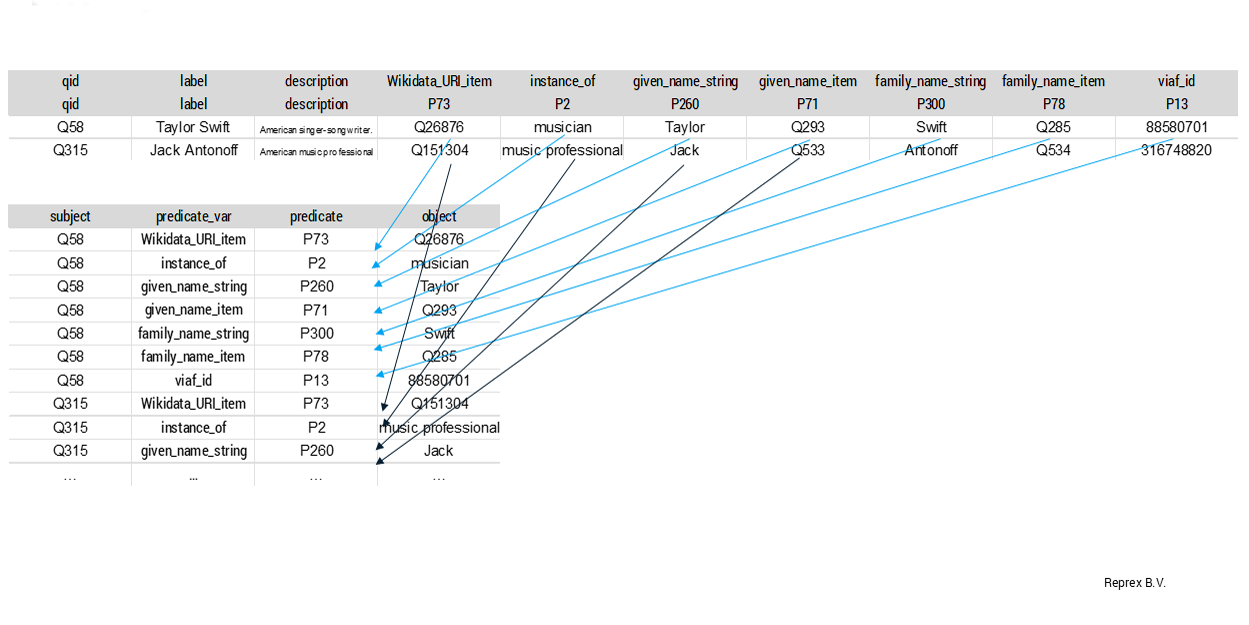
\includegraphics{png/tidy/pivot_longer_to_statements_dual_heading_notitle_2x1.png}
\end{center}

\bookmarksetup{startatroot}

\chapter{OpenCollections}\label{opencollections}

\texttt{OpenCollections} aims to provide a high degree of technical,
syntactic, and semantic interoperability among the data systems of the
partners in the data-sharing space. It imports data (or data maps) into
a graph format, which is optimal for using heterogeneous data sources.
Our innovative solutions aim to make this complex process as fast and
weightless as possible.

The system is built around Wikibase, an information management software
developed by Wikipedia based on the MariaDB relational database
management system. Wikibase manages the world's most extensive open
knowledge graph, Wikidata, and enables users to work in many natural
languages with little or no IT or information science knowledge. Many
use cases, including the creation of the EU Knowledge Graph, inspired us
because Wikibase has a much lower learning need than more optimised
graph database management systems.

\texttt{OpenCollections} improves the Wikibase experience with automated
data-importing components with suitable job aids for users and exporting
tools into more complex graphs that can provide data for training
trustworthy AI systems.

\begin{itemize}
\item[$\boxtimes$]
  We understand the importance of compatibility. That's why we provide
  tools for mass importing data and schematic information from existing
  relational database management systems like MySQL, PostgreSQL, or
  simpler, spreadsheet-based data sources. This reassures our users that
  OpenCollections can seamlessly integrate with their existing systems,
  providing a secure and confident data management experience.
\item[$\boxtimes$]
  We provide training and job aids for manual data processes to keep
  partners' domain-level experts in the loop and provide human agency
  and oversight for trustworthy AI systems.
\item[$\boxtimes$]
  We create a model supported by automation that translates the data
  held in Wikibase to standard machine-actionable ontologies like CIDOC,
  EDM, RiC, and DCAT-AP.
\end{itemize}

\section{Going Beyond Wikibase}\label{going-beyond-wikibase}

Our system is inspired by the WB-CIDOC model developed at the University
of Helsinki for translating knowledge stored in Wikibase into the
statements described with the CIDOC ontology used by intelligent
cultural heritage systems (Kesäniemi, Koho, and Hyvönen 2022). CIDOC is
a modern, events-based ontology that allows building trustworthy
inference and deduction AI engines.

The WB-CIDOC provides rules for writing data into Wikibase in a way that
translates correctly into an event-based model, but we find its use
counter-intuitive and laborious for domain expert data curators.

Most domain experts would think that a biographical entity of
\texttt{Albert\ Einstein} should have a birthday property with the date
of \texttt{March\ 14,\ 1879}, while an event-based ontology would create
first an abstract event, the \texttt{Birth\ of\ Albert\ Einstein}, with
a timespan of \texttt{March\ 14,\ 1879,\ 0:00} to \texttt{23.59}. It is
far easier to search for parallel events in this time window or connect
further information--- like persons present at birth, certificates
created, etc.---than to connect this information to a simple, literal
date.

Domain-level experts like copyright specialists, ESG experts,
musicologists, bank professionals, and other users usually need formal
computer- or information science training and find the entity-based
approach closer to real-world experience. We design our knowledge-base
instances with hooks for more complex knowledge-base ontologies. This
allows our users to review the information in a natural, entity-based
format; our intelligent applications translate the information to more
complex structures, such as event-based conceptual models, to allow more
reasoning capacity for our AI systems.

\subsection{Translation to more complex data
models}\label{translation-to-more-complex-data-models}

Our system is inspired by the WB-CIDOC model developed at the University
of Helsinki for translating knowledge stored in Wikibase into the
statements described with the CIDOC ontology used by intelligent
cultural heritage systems (Kesäniemi, Koho, and Hyvönen 2022). CIDOC is
a modern, events-based ontology that allows building trustworthy
inference and deduction AI engines.

The WB-CIDOC provides rules for writing data into Wikibase in a way that
translates correctly into an event-based model, but we find its use
counter-intuitive and laborious for domain expert data curators.

Most domain experts would think that a biographical entity of
\texttt{Albert\ Einstein} should have a birthday property with the date
of \texttt{March\ 14,\ 1879}, while an event-based ontology would create
first an abstract event, the \texttt{Birth\ of\ Albert\ Einstein}, with
a timespan of \texttt{March\ 14,\ 1879,\ 0:00} to \texttt{23.59}. It is
far easier to search for parallel events in this time window or connect
further information--- like persons present at birth, certificates
created, etc.---than to connect this information to a simple, literal
date.

\begin{tcolorbox}[enhanced jigsaw, opacityback=0, bottomrule=.15mm, rightrule=.15mm, toptitle=1mm, breakable, colbacktitle=quarto-callout-note-color!10!white, colback=white, title=\textcolor{quarto-callout-note-color}{\faInfo}\hspace{0.5em}{Note}, leftrule=.75mm, toprule=.15mm, left=2mm, arc=.35mm, colframe=quarto-callout-note-color-frame, coltitle=black, titlerule=0mm, bottomtitle=1mm, opacitybacktitle=0.6]

Domain-level experts like copyright specialists, ESG experts,
musicologists, bank professionals, and other users usually need formal
computer- or information science training and find the entity-based
approach closer to real-world experience. We design our knowledge-base
instances with hooks for more complex knowledge-base ontologies. This
allows our users to review the information in a natural, entity-based
format; our intelligent applications translate the information to more
complex structures, such as event-based conceptual models, to allow more
reasoning capacity for our AI systems.

\end{tcolorbox}

\subsection{Record-keeping and
retention}\label{record-keeping-and-retention}

National archives play a crucial role in preserving the collective
memory and history of a nation. Connecting national archives to
institutional enterprise record-keeping systems has many advantages.

\begin{enumerate}
\def\labelenumi{\arabic{enumi}.}
\item
  \textbf{Contextualising institutional or enterprise records}: Private
  organisations and users cannot copy all legally or historically
  relevant documents in their inventory. Connecting to memory
  institutions, such as records or legal databases, allows one to find
  precedents and understand one and one's own historical records in
  context without the need to hoard information on an excessive scale.
  Just the way we do not need to burden our office bookshelves with
  bilingual dictionaries or printed copies of changing regulations, we
  can further lower the burden by making our records system compatible
  with national records.
\item
  \textbf{Record retention and public archiving} is a regulated process
  that serves as the foundation of many business processes' regulatory
  or assurance oversight. Businesses often must deposit copies of
  legally important disclosures and certificates at public bodies.
  Larger institutions, primarily if they work for the public benefit,
  usually have a legal mandate to place some of their documents into a
  public archive. Private persons and companies often donate documents
  to such archives when they want to be credited with their work,
  intellectual property, or the value of their activities.
\end{enumerate}

Because OpenCollections is based around a document-based database, it is
very well suited to support document exchanges between private
institutions (e.g., the exchange of technical and delivery documentation
along the supply chain), public institutions (e.g., the exchange of
public documents), and public-private exchanges.

We provide mappings, software tools and training to apply Records in
Context (RiC), a novel ontology released in 2023 after over a decade's
work to replace the four international standards on archiving. The last
international standards on the topic were created before the commercial
Internet; RiC provides backwards compatibility to millennia of
historical records, corporate document inventories, and physical data
vaults on one hand, and opens up the use of modern knowledge graphs to
link information in the archives with your documents in use. RiC is the
gateway to corporate and institutional textual big data.

\subsection{Data catalogues, and the meaning of data
tables}\label{data-catalogues-and-the-meaning-of-data-tables}

Following the DCAT-AP specification of the EU Open Data Portal and
Stat-DCAT-AP to offer full compatibility with European statistical
portals and open data portals, we translate information about datasets,
data codes and structures, and variable descriptions. This translation
works with few limitations for global resources beyond Europe. It
connects corporate or institutional datasets and accounts with
statistical and national accounts data from public sources, offering
unparalleled ease in creating economic or sustainability-controlling
applications.

\subsection{Collections and
inventories}\label{collections-and-inventories}

\bookmarksetup{startatroot}

\chapter*{References}\label{references}
\addcontentsline{toc}{chapter}{References}

\markboth{References}{References}

\phantomsection\label{refs}
\begin{CSLReferences}{1}{0}
\bibitem[\citeproctext]{ref-allamanis_suggesting_method_class_names_2015}
Allamanis, Miltiadis, Barr, Earl T., Bird, Christian, and Sutton,
Charles. 2015. {``Suggesting Accurate Method and Class Names.''} In
\emph{Proceedings of the 2015 10th Joint Meeting on Foundations of
Software Engineering}, 38--49. Bergamo, Italy.
\url{https://dl-acm-org.proxy.uba.uva.nl/doi/abs/10.1145/2786805.2786849}.

\bibitem[\citeproctext]{ref-berners-lee_uri_generic_syntax_2005}
Berners-Lee, Tim, Roy T. Fielding, and Larry M. Masinter. 2005.
{``Uniform Resource Identifier ({URI}): Generic Syntax.''} Request for
Comments {RFC} 3986. Internet Engineering Task Force.
\url{https://doi.org/10.17487/RFC3986}.

\bibitem[\citeproctext]{ref-berners-lee_semantic_web_2001}
Berners-Lee, Tim, James Hendler, and Ora Lassila. 2001. {``The Semantic
Web.''} Scientific American, Incorporated.

\bibitem[\citeproctext]{ref-dallas_digital_curation_2016}
Dallas, Costis. 2016. {``Digital Curation Beyond the {`Wild Frontier'}:
A Pragmatic Approach.''} \emph{Archival Science} 16 (4): 421--57.
\url{https://doi.org/10.1007/s10502-015-9252-6}.

\bibitem[\citeproctext]{ref-ddi_lifecycle_3-3}
Data Documentation Initiative. 2020. {``DDI Lifecycle {(3.3)}
Documentation.''}
\url{https://ddi-lifecycle-documentation.readthedocs.io/en/latest/index.html}.

\bibitem[\citeproctext]{ref-diefenbach_wikibase_2021}
Diefenbach, Dennis, Max de Wilde, and Samantha Alipio. 2021. {``Wikibase
as an Infrastructure for Knowledge Graphs: The {EU} Knowledge Graph.''}
In \emph{{ISWC} 2021}. Online, France.
\url{https://hal.science/hal-03353225}.

\bibitem[\citeproctext]{ref-harpring_baca_categorizing_art_2016}
Harpring, Patricia, and Murtha Baca. 2016. {``19. Art Vocabulary:
Categorizing Works of Art.''} In \emph{Handbuch Sprache in Der
Kunstkommunikation}, edited by Heiko Hausendorf and Marcus Müller,
425--54. Berlin, Boston: De Gruyter.
\url{https://doi.org/doi:10.1515/9783110296273-020}.

\bibitem[\citeproctext]{ref-hartman_john_smith_et_al}
Hartman, Lee. n.d. {``John Smith Et Al.: Some Observations on How the 20
Most Popular First Names Combine with the 20 Most Popular Surnames in
the United States.''} Accessed August 16, 2024.
\url{https://web.archive.org/web/20190225042148/http://mypage.siu.edu/lhartman/johnsmith.html}.

\bibitem[\citeproctext]{ref-ddi-rdf_discovery_2024}
Hartmann, Thomas, Sarven Capadisli, Franck Cotton, Richard Cyganiak,
Arofan Gregory, Benedikt Kämpgen, Olof Olsson, Heiko Paulheim, Joachim
Wackerow, and Benjamin Zapilko. 2024. {``{DDI}-{RDF} Discovery
Vocabulary. A Vocabulary for Publishing Metadata about Data Sets
(Research and Survey Data) into the Web of Linked Data.''} Edited by
Thomas Hartmann, Richard Cyganiak, Joachim Wackerow, and Benjamin
Zapilko. W3C.
\url{https://rdf-vocabulary.ddialliance.org/discovery.html}.

\bibitem[\citeproctext]{ref-iso_isni_2012}
ISO. 2012. {``International Standard Musical Work Code ({ISNI}). {ISO}
27729:2012.''} International Organization for Standardization.
\url{https://www.iso.org/standard/44292.html}.

\bibitem[\citeproctext]{ref-iso_19941_2017}
---------. 2017. {``{ISO}/{IEC} 19941:2017(en), Information Technology
--- Cloud Computing --- Interoperability and Portability.''}
London:United Kingdom: International Organization for Standardization.
\url{https://www.iso.org/obp/ui/\#iso:std:iso-iec:19941:ed-1:v1:en}.

\bibitem[\citeproctext]{ref-iso_22624_2020}
---------. 2020. {``{ISO}/{IEC} 22624:2020(en), Information Technology
--- Cloud Computing --- Taxonomy Based Data Handling for Cloud
Services.''} London:United Kingdom: {International Organization for
Standardization}.
\url{https://www.iso.org/obp/ui/en/\#iso:std:iso-iec:22624:ed-1:v1:en}.

\bibitem[\citeproctext]{ref-iso_2382_2015}
---------. 2023. {``{ISO}/{IEC} 2382:2015(en), Information Technology
--- Vocabulary.''} London:United Kingdom: International Standards
Organisation.
\url{https://www.iso.org/obp/ui/en/\#iso:std:iso-iec:2382:ed-1:v2:en}.

\bibitem[\citeproctext]{ref-kesaniemi_wb_cidoc_2022}
Kesäniemi, Joonas, Mikko Koho, and Eero Hyvönen. 2022. {``Using Wikibase
for Managing Cultural Heritage Linked Open Data Based on {CIDOC}
{CRM}.''} In \emph{New Trends in Database and Information Systems},
edited by Silvia Chiusano, Tania Cerquitelli, Robert Wrembel, Kjetil
Nørvåg, Barbara Catania, Genoveva Vargas-Solar, and Ester Zumpano,
542--49. Cham: Springer International Publishing.
\url{https://doi.org/10.1007/978-3-031-15743-1_49}.

\bibitem[\citeproctext]{ref-meeus_2022_7238006}
Meeus, Sofie, Wouter Addink, Donat Agosti, Christos Arvanitidis, Bachir
Balech, Mathias Dillen, Mariya Dimitrova, et al. 2022.
{``{Recommendations for interoperability among infrastructures}.''}
\emph{Research Ideas and Outcomes} 8 (October).
\url{https://doi.org/10.3897/rio.8.e96180}.

\bibitem[\citeproctext]{ref-paskin_toward_1999}
Paskin, N. 1999. {``Toward Unique Identifiers.''} \emph{Proceedings of
the {IEEE}} 87 (7): 1208--27. \url{https://doi.org/10.1109/5.771073}.

\bibitem[\citeproctext]{ref-paskin_identification_2003}
Paskin, Norman. 2003. {``Identification and Metadata.''} In
\emph{Digital Rights Management: Technological, Economic, Legal and
Political Aspects}, 26--61. Lecture Notes in Computer Science 2770.
Berlin: Springer.

\bibitem[\citeproctext]{ref-pomerantz_metadata_2015}
Pomerantz, Jeffrey. 2015. \emph{Metadata}. The {MIT} Press Essential
Knowledge Series. Cambridge, {MA}, {USA}: {MIT} Press.

\bibitem[\citeproctext]{ref-GSIM_v20_2014}
UNECE. 2014. {``Generic Statistical Information Model. {GSIM} V2.0
Documents. {UNECE} Statswiki.''} 2014.
\url{https://statswiki.unece.org/display/gsim/GSIM+v2.0+documents}.

\bibitem[\citeproctext]{ref-vardigan_DDI_2008}
Vardigan, Mary, Pascal Heus, and Wendy Thomas. 2008. {``Data
Documentation Initiative: Toward a Standard for the Social Sciences.''}
\emph{International Journal of Digital Curation} 3 (1): 107--13.

\end{CSLReferences}

\cleardoublepage
\phantomsection
\addcontentsline{toc}{part}{Appendices}
\appendix

\chapter{Question Bank Items In Wikibase}\label{sec-questionbank}

In this guide you are going to learn how to feed different types of
questions and information related to them to Wikibase.

First, you will read about how to load into Wikibase different type of
questions. Second, you will learn about different types of information
and how to link them to your question. Last, you will see how to add
different translations to a question.

The concept behind the workflows follows the DDI-Lifecycle framework.
The DDI lifecycle model is designed to support the documentation and
management of data throughout its entire lifecycle, ensuring that data
can be effectively shared, reused, and preserved. DDI-Lifecycle is not
yet available in RDF. Some elements of DDI are standardised; others are
not. Whenever possible, we use the standardised \emph{DDI-RDF Discovery
Vocabulary}; when no such ontology is present, we create our
interpretation of DDI Hartmann et al. (2024).

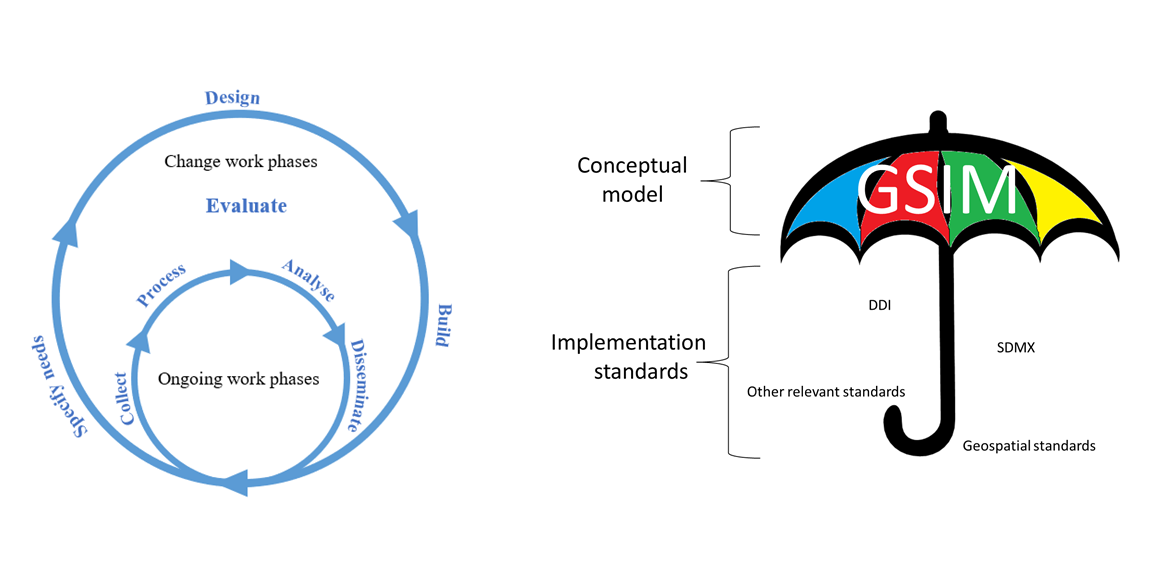
\includegraphics{png/datamodels/gsim.png}

DDI is part of the \textbf{General Statistical Information Model}
(GSIM)(UNECE 2014), which accompanies the \textbf{Generic Statistical
Business Process Model} (GSBPM) as an international standard model that
``describes and defines the set of business processes needed to produce
official statistics.'' We use the conceptualisation of GSIM so that our
results will be similar in quality to official statistics; of course,
similar processes allow us to create products that combine well with
official statistical products.

\begin{figure}[H]

{\centering 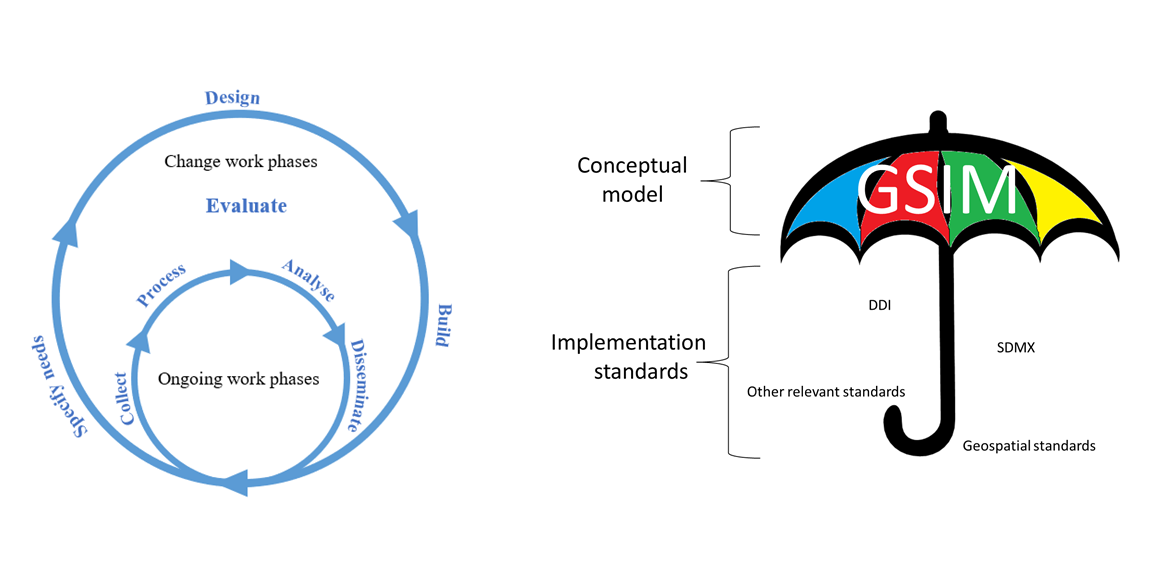
\includegraphics{png/datamodels/gsim.png}

}

\caption{The two implementation standards, DDI and SDMX ensures that our
observatories can work together with statistical offices, or respectable
social sciences data repositories.}

\end{figure}%

Applying the \emph{Data Documentation Initiatve} (DDI) will ensure that
we will remain compatible with official statistical microdata and
metadata services and other social sciences archives, like GESIS, the
official data archive of all European Commission-mandated survey
research dating back over 50 years (Vardigan, Heus, and Thomas 2008).

\section{Need for Questions}\label{need-for-questions}

The need for questions arises from the fact that you want to collect
some data systematically, either in an online or face-to-face
questionnaire, in a structured interview, or in making data requests to
an API or a form to record repeated answers to this question. After
statistical manipulations, such as summarising and averaging, the
responses will create empirical variables in a dataset. You can rely on
existing data and expand your knowledge utilising already collected
(open) data if you use the same questions that other researchers or
statisticians have used before you.

Without addressing the theory of data harmonisation, these are the steps
you are likely to make:

\begin{enumerate}
\def\labelenumi{\arabic{enumi}.}
\tightlist
\item
  For example, if you need data on reusable plastic bags, you need to
  find a widely shared definition of \texttt{plastic},
  \texttt{reusability} and \texttt{bags}.
\item
  You should consult a database or a question bank to find out if others
  have already asked about reusable plastic bags.
\item
  If you formulate a questionnaire using the exact wording and answering
  options as earlier surveys on attitudes to reusable plastic bags, you
  will be able to compare the results. So, you need access to question
  forms (question texts) and answer options.
\item
  If you work on an international project or want a global comparison,
  you will need to ensure that the question texts and answer options are
  translated very similarly and understood equally in different
  languages.
\item
  As a practical last step, the responses must be coded the same way as
  in international data repositories; for example, female respondents
  are coded with \texttt{F} in most statistical data repositories, even
  if the word `female' may start with a different letter in many
  languages.
\end{enumerate}

Our question bank is designed to be searchable by concepts, question
types, question labels or question texts.

\section{Question Types}\label{question-types}

What is a survey question after all? DDI organises questions into 3+1
hierarchical levels.

\begin{itemize}
\item[$\boxtimes$]
  \texttt{Question}: A question and its answer options formulated in at
  least one natural language, for example,
  \texttt{Please\ tell\ me\ to\ what\ extent\ you\ agree\ or\ disagree\ with\ the\ following\ statement:}
  \texttt{“I\ trust\ that\ products\ carrying\ the\ EU\ ecolabel\ are\ environmentally-friendly.”}
  \texttt{{[}\ {]}\ Totally\ agree\ {[}\ {]},\ Tend\ to\ agree\ {[}\ {]},\ Tend\ to\ disagree\ {[}\ {]},\ Totally\ disagree\ {[}\ {]},\ DK}.
  In this example DK refers to declined to comment on the question, or a
  refusal to answer this question.
\item[$\boxtimes$]
  \texttt{QuestionItem}: the concept (i.e., unemployment, or plastic
  bags) being measured by the question, text for the question, response
  domain information, clarifying instructions, external aids (clarifying
  objects used in presenting the question to the respondent), Input and
  Output Parameters and Bindings, allowed response cardinality and
  estimation of the time required to respond.
\item[$\boxtimes$]
  \texttt{QuestionBlock}: This structure is intended to bundle together
  a set of questions (items and/or grids) that have meaning only about a
  specified object expressed as the evaluation material. This form of
  question set is common in educational testing where a text, image, or
  other material is provided, and the respondent is asked questions
  specific to the material. For example, a portion of a play script is
  provided, and the respondent is asked questions concerning the
  dialogue and/or stage directions provided in the script. Note that the
  intent of QuestionBlock is not to bundle together a set of questions
  that are commonly used together or used in a specified order.
\item[$\boxtimes$]
  \texttt{QuestionGroup} is only for administrative purposes.
\end{itemize}

\subsection{Model question}\label{model-question}

One other way to make questions and resulting responses and their
statistically processed variables comparable is to ask questions about
different concepts in a same way? A standard quesiton in a Cultural
Access and Participation Survey is:

\texttt{How\ many\ times\ in\ the\ past\ 12\ months\ have\ you\ been\ to\ ...}
\texttt{...\ a\ concert?} \texttt{...\ cinema?} \texttt{...\ church?}

While people may have recollection biases about the 12 months, and may
use a bit differently the concept of concert or cinema, because of the
same syntax, context, we can assume that their responses are comparable.
In this case,
\texttt{How\ many\ times\ in\ the\ past\ 12\ months\ have\ you\ been\ to\ ...}
is a model question.

A \href{https://reprexbase.eu/demowiki/index.php?title=Item:Q126}{model
question} is a question template that can create simple questions or
question items in question grids or blocks.

\begin{itemize}
\tightlist
\item
  URI:
  \href{https://reprexbase.eu/demowiki/index.php?title=Item:Q127}{Q127}
\item
  label: \texttt{Trust\ in\ EU\ ECOLABEL\ {[}model{]}}
\item
  questionText (description):
  \texttt{Please\ tell\ me\ to\ what\ extent\ you\ agree\ or\ disagree\ with\ the\ following\ statement:\ “I\ trust\ that\ products\ carrying\ the\ EU\ ecolabel\ are\ environmentally-friendly.”\ {[}\ {]}\ scale}
\end{itemize}

And a question based on a model question, taken from

\begin{itemize}
\item
  QID: \url{https://reprexbase.eu/demowiki/index.php?title=Item:Q111}
\item
  label: \texttt{Trust\ in\ EU\ ECOLABEL}
\item
  questionText (description):
  \texttt{Please\ tell\ me\ to\ what\ extent\ you\ agree\ or\ disagree\ with\ the\ following\ statement:}
  \texttt{“I\ trust\ that\ products\ carrying\ the\ EU\ ecolabel\ are\ environmentally-friendly.”}
  \texttt{{[}\ {]}\ Totally\ agree\ {[}\ {]},\ Tend\ to\ agree\ {[}\ {]},\ Tend\ to\ disagree\ {[}\ {]},\ Totally\ disagree\ {[}\ {]},\ DK}
\item
  variable representation:
  \href{https://reprexbase.eu/demowiki/index.php?title=Item:Q116}{scale
  representation base type}
\item
  study (DDI):
  \href{https://reprexbase.eu/demowiki/index.php?title=Item:Q139}{Eurobarometer
  88.1 (2017)}
\end{itemize}

Our model questions follow one of the following formats:

\begin{itemize}
\tightlist
\item
  \texttt{questionText\ (description)}, \texttt{{[}\ {]}}
  \texttt{concept}, where the question connects to a concept, such as
  \href{https://reprexbase.eu/demowiki/index.php?title=Item:Q131}{environmental
  protection (Q131)}.
\item
  \texttt{questionText\ (description)}, \texttt{{[}\ {]}}
  \texttt{scale}, where the answers are on a scale, for example
  \href{https://reprexbase.eu/demowiki/index.php?title=Item:Q123}{Estimated
  number of employees in FTE {[}model{]} (Q123)}
\item
  \texttt{questionText\ (description)}, \texttt{{[}\ {]}}
  \texttt{category}, where the answer options are categories, for
  example:
  \href{https://reprexbase.eu/demowiki/index.php?title=Item:Q112}{Reduced
  use of single use plastic bags {[}model{]} (Q112)}
\item
  \texttt{questionText\ (description)}, \texttt{{[}\ {]}}
  \texttt{ranking}, where the respondent has to create a rank from the
  answer options, for example:
  \href{https://reprexbase.eu/demowiki/index.php?title=Item:Q143}{Important
  environmental issue {[}model{]} (Q143)}
\item
  \texttt{questionText\ (description)}, \texttt{{[}\ {]}}
  \texttt{concept,} \texttt{{[}\ {]}\ scale,} where beside the model
  question there are other sub-questions as well, for example:
  \href{https://reprexbase.eu/demowiki/index.php?title=Item:Q128}{Important
  for reduction of plastic {[}model{]} (Q128)}
\end{itemize}

Based on the DDI-Lifecycle model we could generate differently
structured model questions, and if there will be user need, we will
introduce further question templates.

The DDI-Discovery ontology requires the questions to take this format:

\begin{quote}
\emph{Please tell me to what extent you agree or disagree with the
following statement: ``I trust that products carrying the EU ecolabel
are environmentally-friendly.'' {[} {]} Totally agree {[} {]}, Tend to
agree {[} {]}, Tend to disagree {[} {]}, Totally disagree {[} {]}, DK}.
\end{quote}

This is a good representation to for an existing questionnaire, but it
is not really good for a questionbank, because in some cases, the
agreement scale may be a 3-level, in others, a 5-level agreement scale:

\begin{quote}
\emph{Please tell me to what extent you agree or disagree with the
following statement: ``I trust that products carrying the EU ecolabel
are environmentally-friendly.'' {[} {]}, Agree {[} {]}, {[} {]},
Disagree {[} {]}, DK}
\end{quote}

We can argue that the responses are still comparable, but
\texttt{{[}\ {]}\ Totally\ agree\ {[}\ {]},\ Tend\ to\ agree\ {[}\ {]}}
should be added together for a broader \texttt{{[}\ {]}\ Agree} category
if one survey uses the 5-scale version of the response scale while the
other uses the 3-scale (agree, disagree, decline) version.

This is why we separately record the model question, the subquestions
and the answer options.

\subsection{Simple, Multiple Choice and Matrix
Questions}\label{simple-multiple-choice-and-matrix-questions}

Different question types have different elements. Some questions consist
of one question, others have group questions and several sub-questions.

A question might consists of the following elements:

\texttt{{[}Model\ question{]}\ +\ \ {[}Question\ Items{]}\ +\ \ {[}Answer\ options{]}}

\begin{itemize}
\item
  All elements should be added separately to the Wikibase
\item
  The format changes based on the type of the question:

  \begin{itemize}
  \tightlist
  \item
    simple question: \texttt{{[}Model\ question{]}\ +\ {[}Answers{]}}
  \item
    multiple choice question:
    \texttt{{[}Model\ question{]}\ +\ {[}Question\ Items{]}}
  \item
    matrix question:
    \texttt{{[}Model\ question{]}\ +\ \ {[}Question\ Items{]}\ +\ \ {[}Answer\ options{]}}
  \end{itemize}
\end{itemize}

Let's see how to load into Wikibase:

\begin{itemize}
\tightlist
\item
  Simple Questions
\end{itemize}

\begin{itemize}
\item
  Matrix Questions
\item
  Multiple Choice Questions
\end{itemize}

\subsubsection{Simple Questions}\label{simple-questions}

In case of Simple Questions there's only one question.

\begin{tcolorbox}[enhanced jigsaw, opacityback=0, bottomrule=.15mm, rightrule=.15mm, toptitle=1mm, breakable, colbacktitle=quarto-callout-note-color!10!white, colback=white, title=\textcolor{quarto-callout-note-color}{\faInfo}\hspace{0.5em}{Note}, leftrule=.75mm, toprule=.15mm, left=2mm, arc=.35mm, colframe=quarto-callout-note-color-frame, coltitle=black, titlerule=0mm, bottomtitle=1mm, opacitybacktitle=0.6]

For a clearer definition, see the
\href{https://rdf-vocabulary.ddialliance.org/discovery.html\#question}{disco:Question}
class.

\end{tcolorbox}

\begin{center}
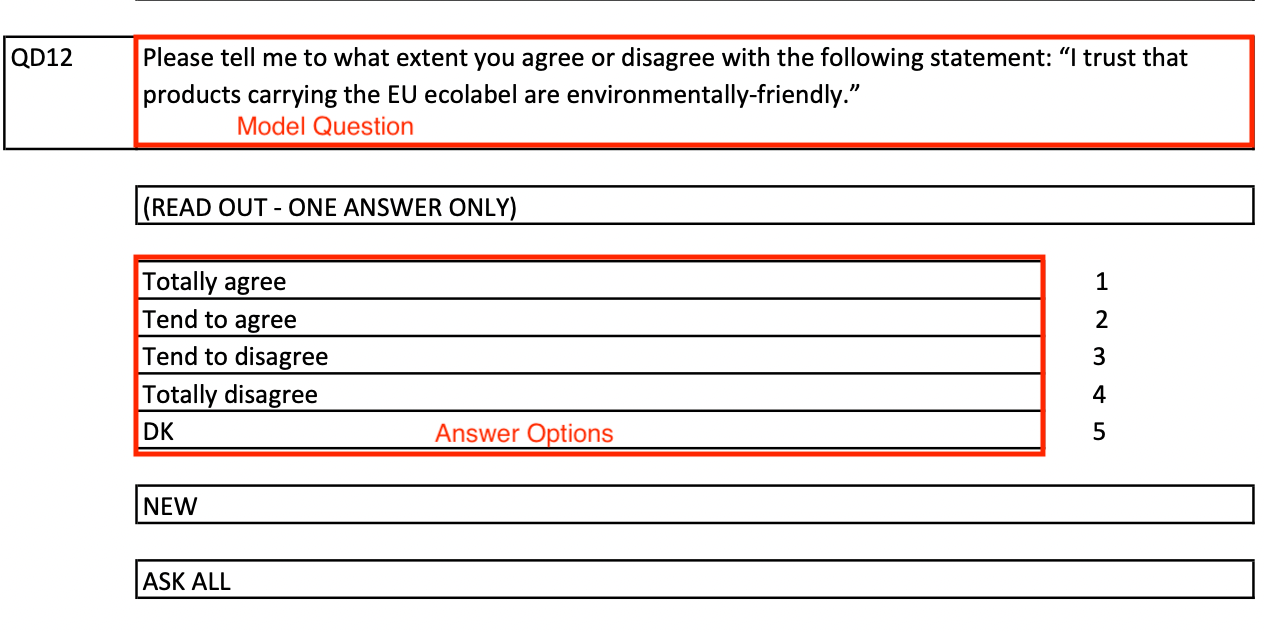
\includegraphics{png/question_to_wikibase/question_simple_2x1.png}
\end{center}
The format of a simple question is:
\texttt{{[}Model\ question{]}\ +\ {[}Answer\ options{]}}

Let's see how to create a simple question entry in Wikibase. Go to
``Special Pages''

\begin{center}
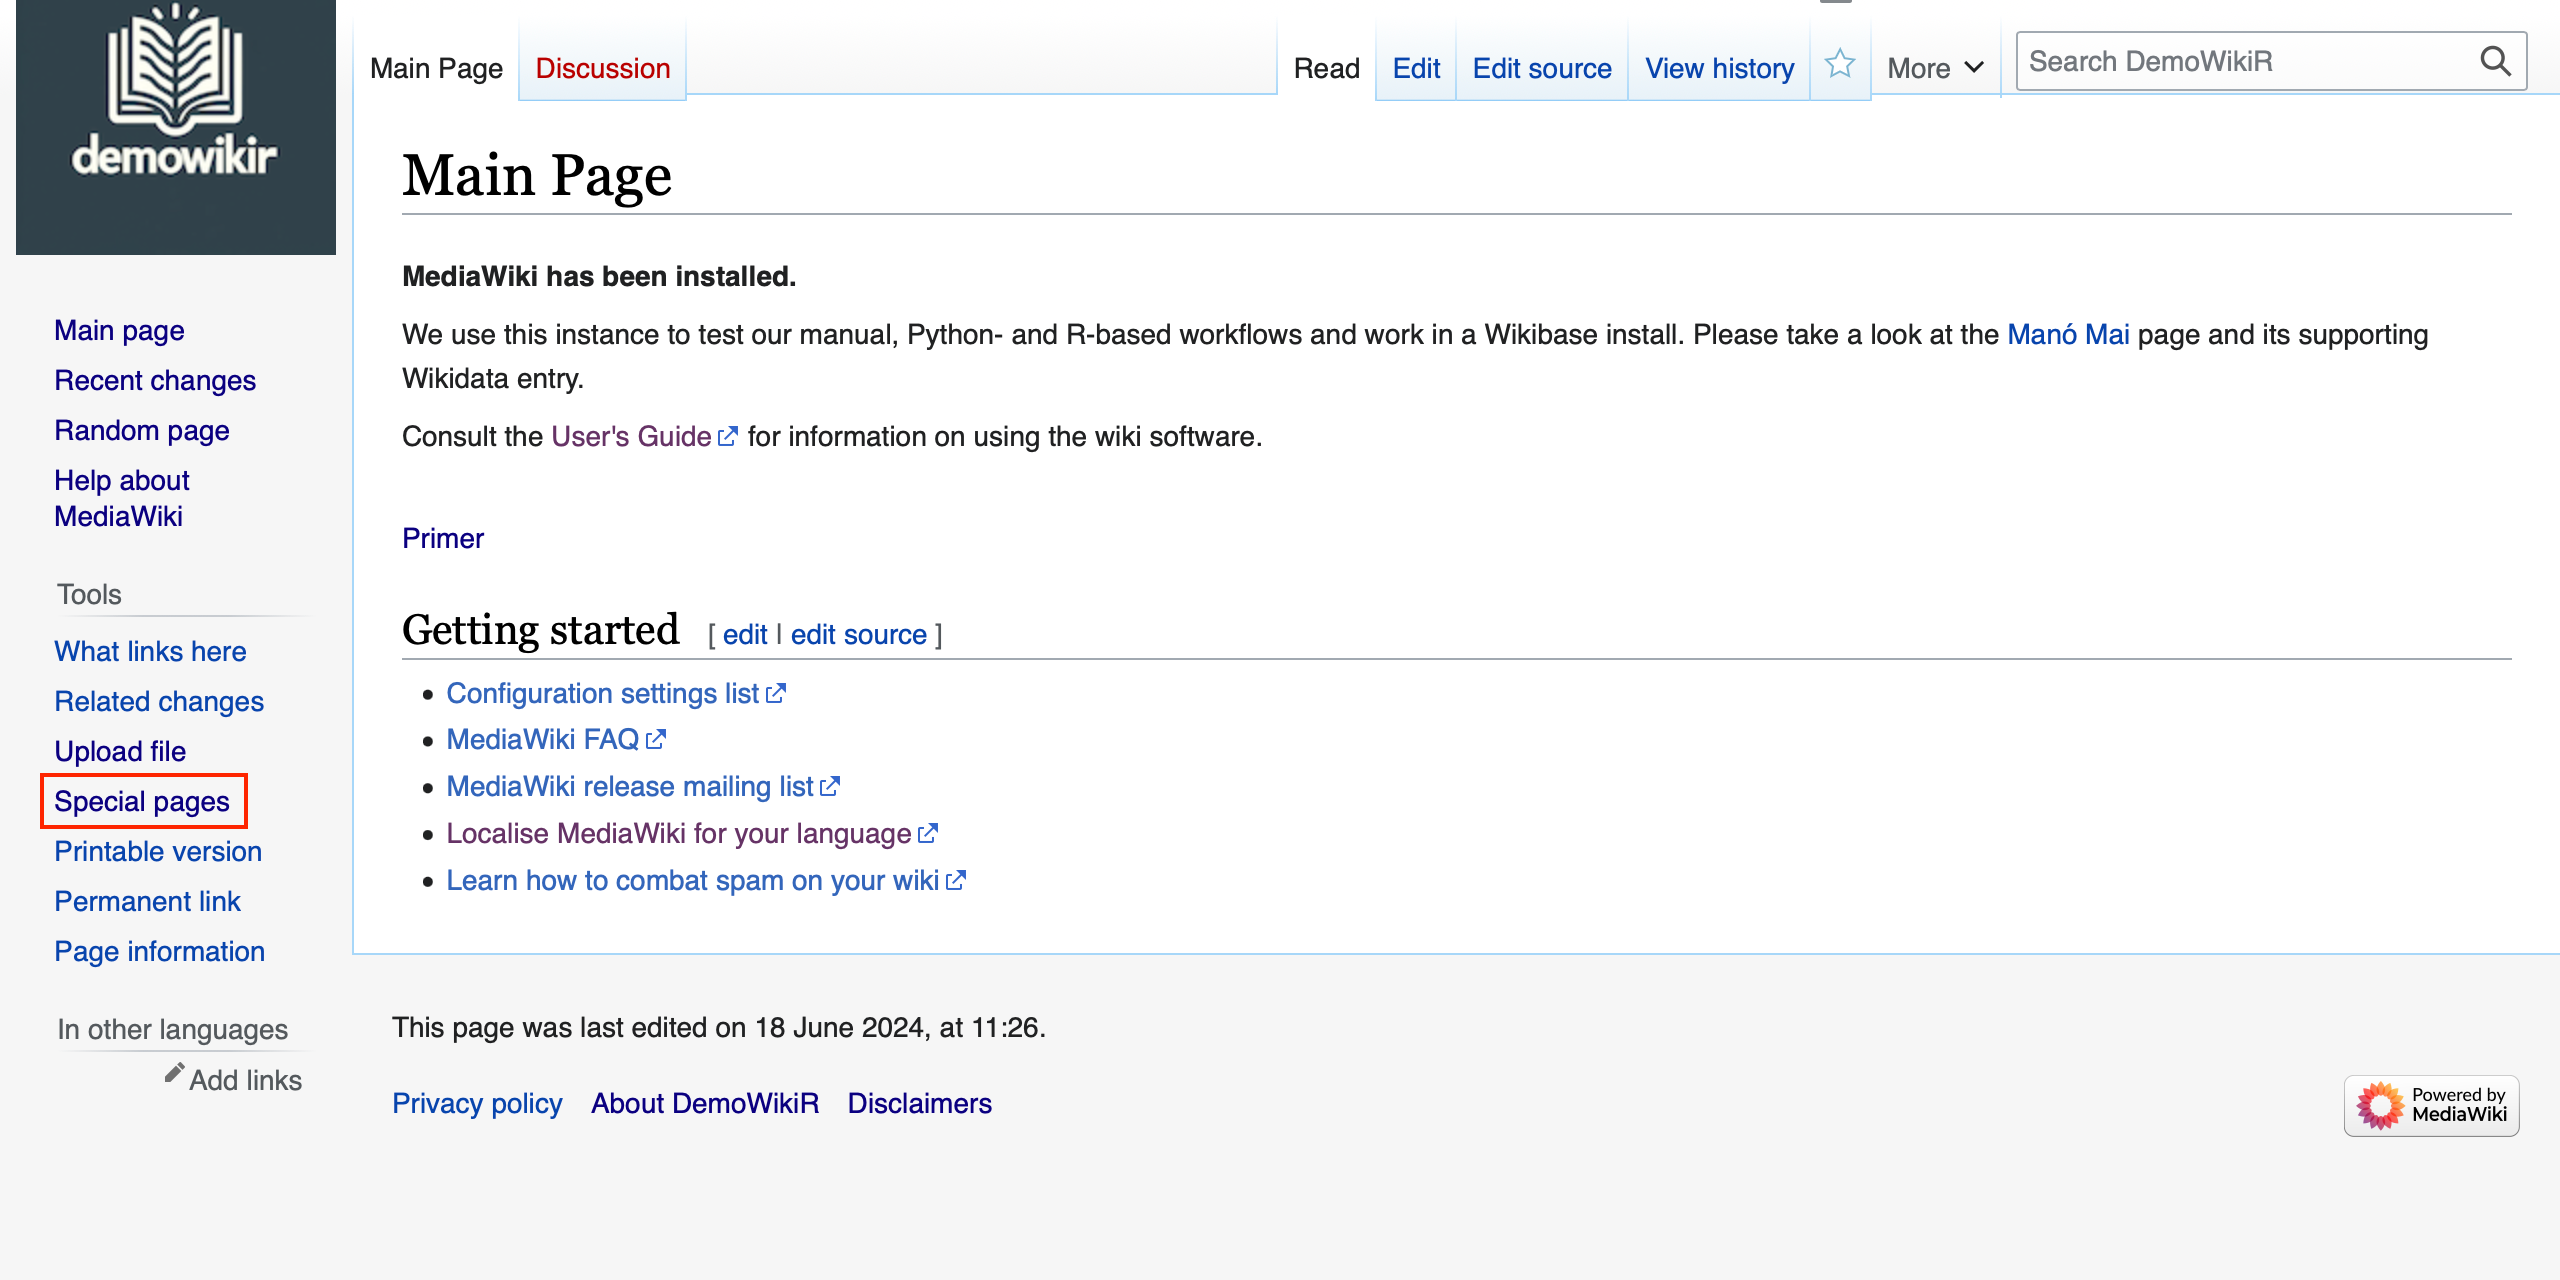
\includegraphics{png/question_to_wikibase/wikidata_specialPages_2x1.png}
\end{center}

Scroll down and select: \texttt{Create\ a\ New\ Item}

\begin{center}
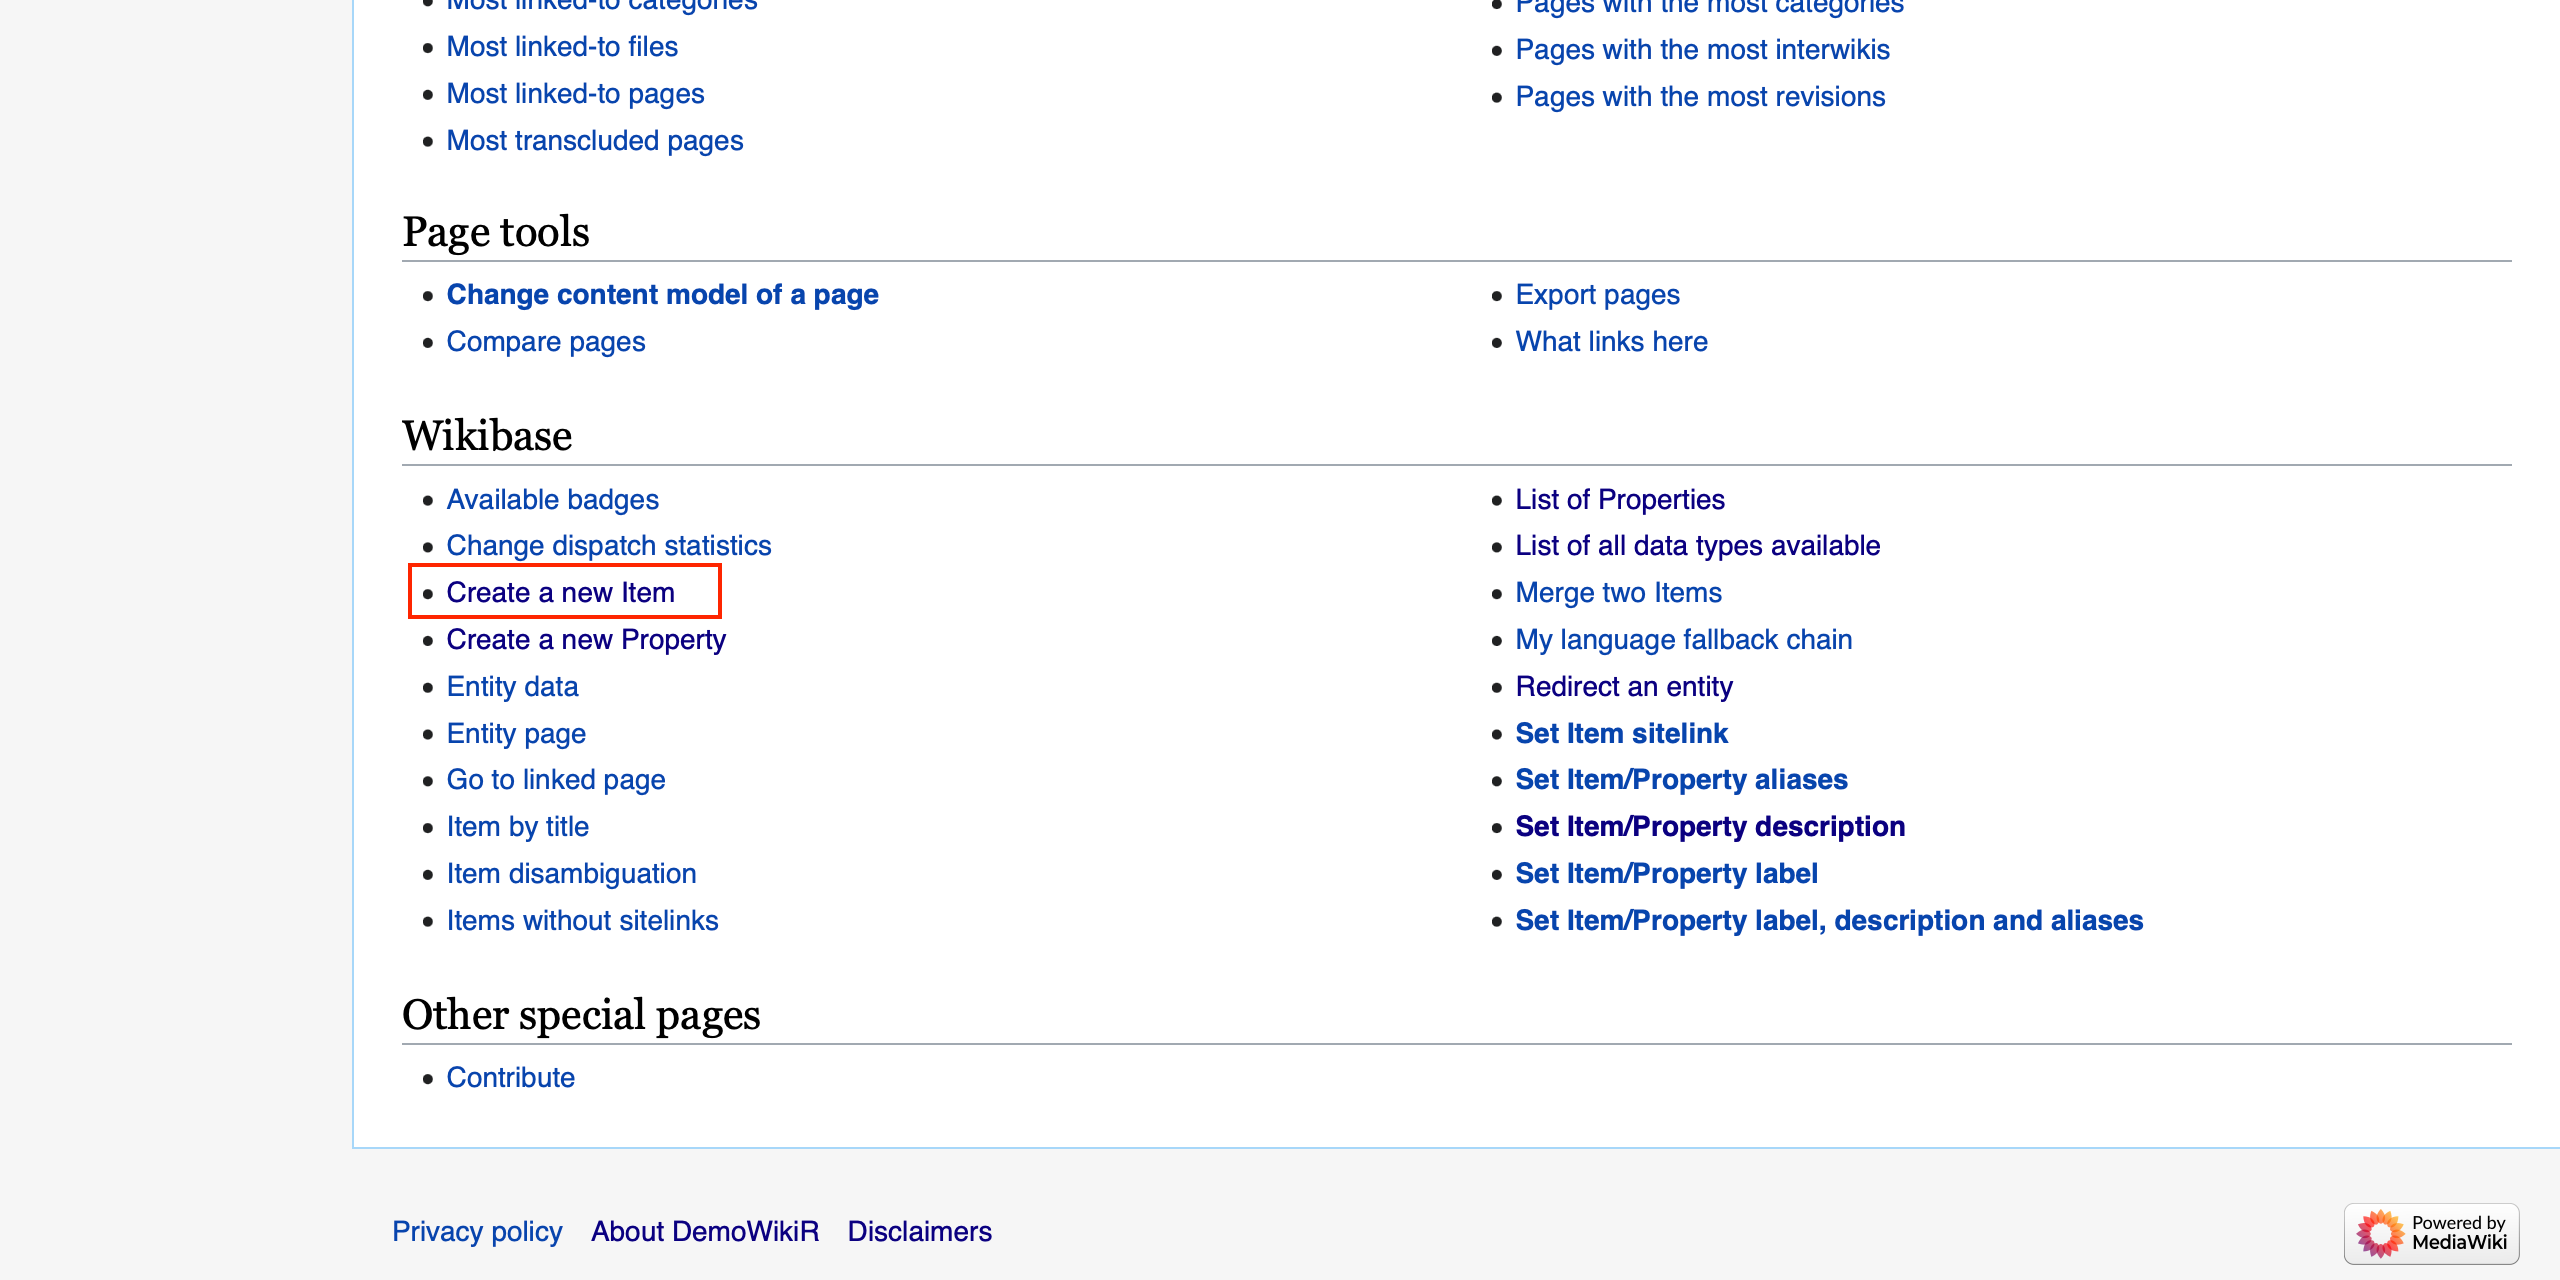
\includegraphics{png/question_to_wikibase/wikibase_addNewItem_2x1.png}
\end{center}

Fill the form with the question's data:

\begin{itemize}
\item
  Language ▷ Choose the language (en)
\item
  Label - Give a short name for the question
\item
  Description - Enter the question itself in the format specified above.
\item
  Aliases - leave it empty
\end{itemize}

\begin{center}
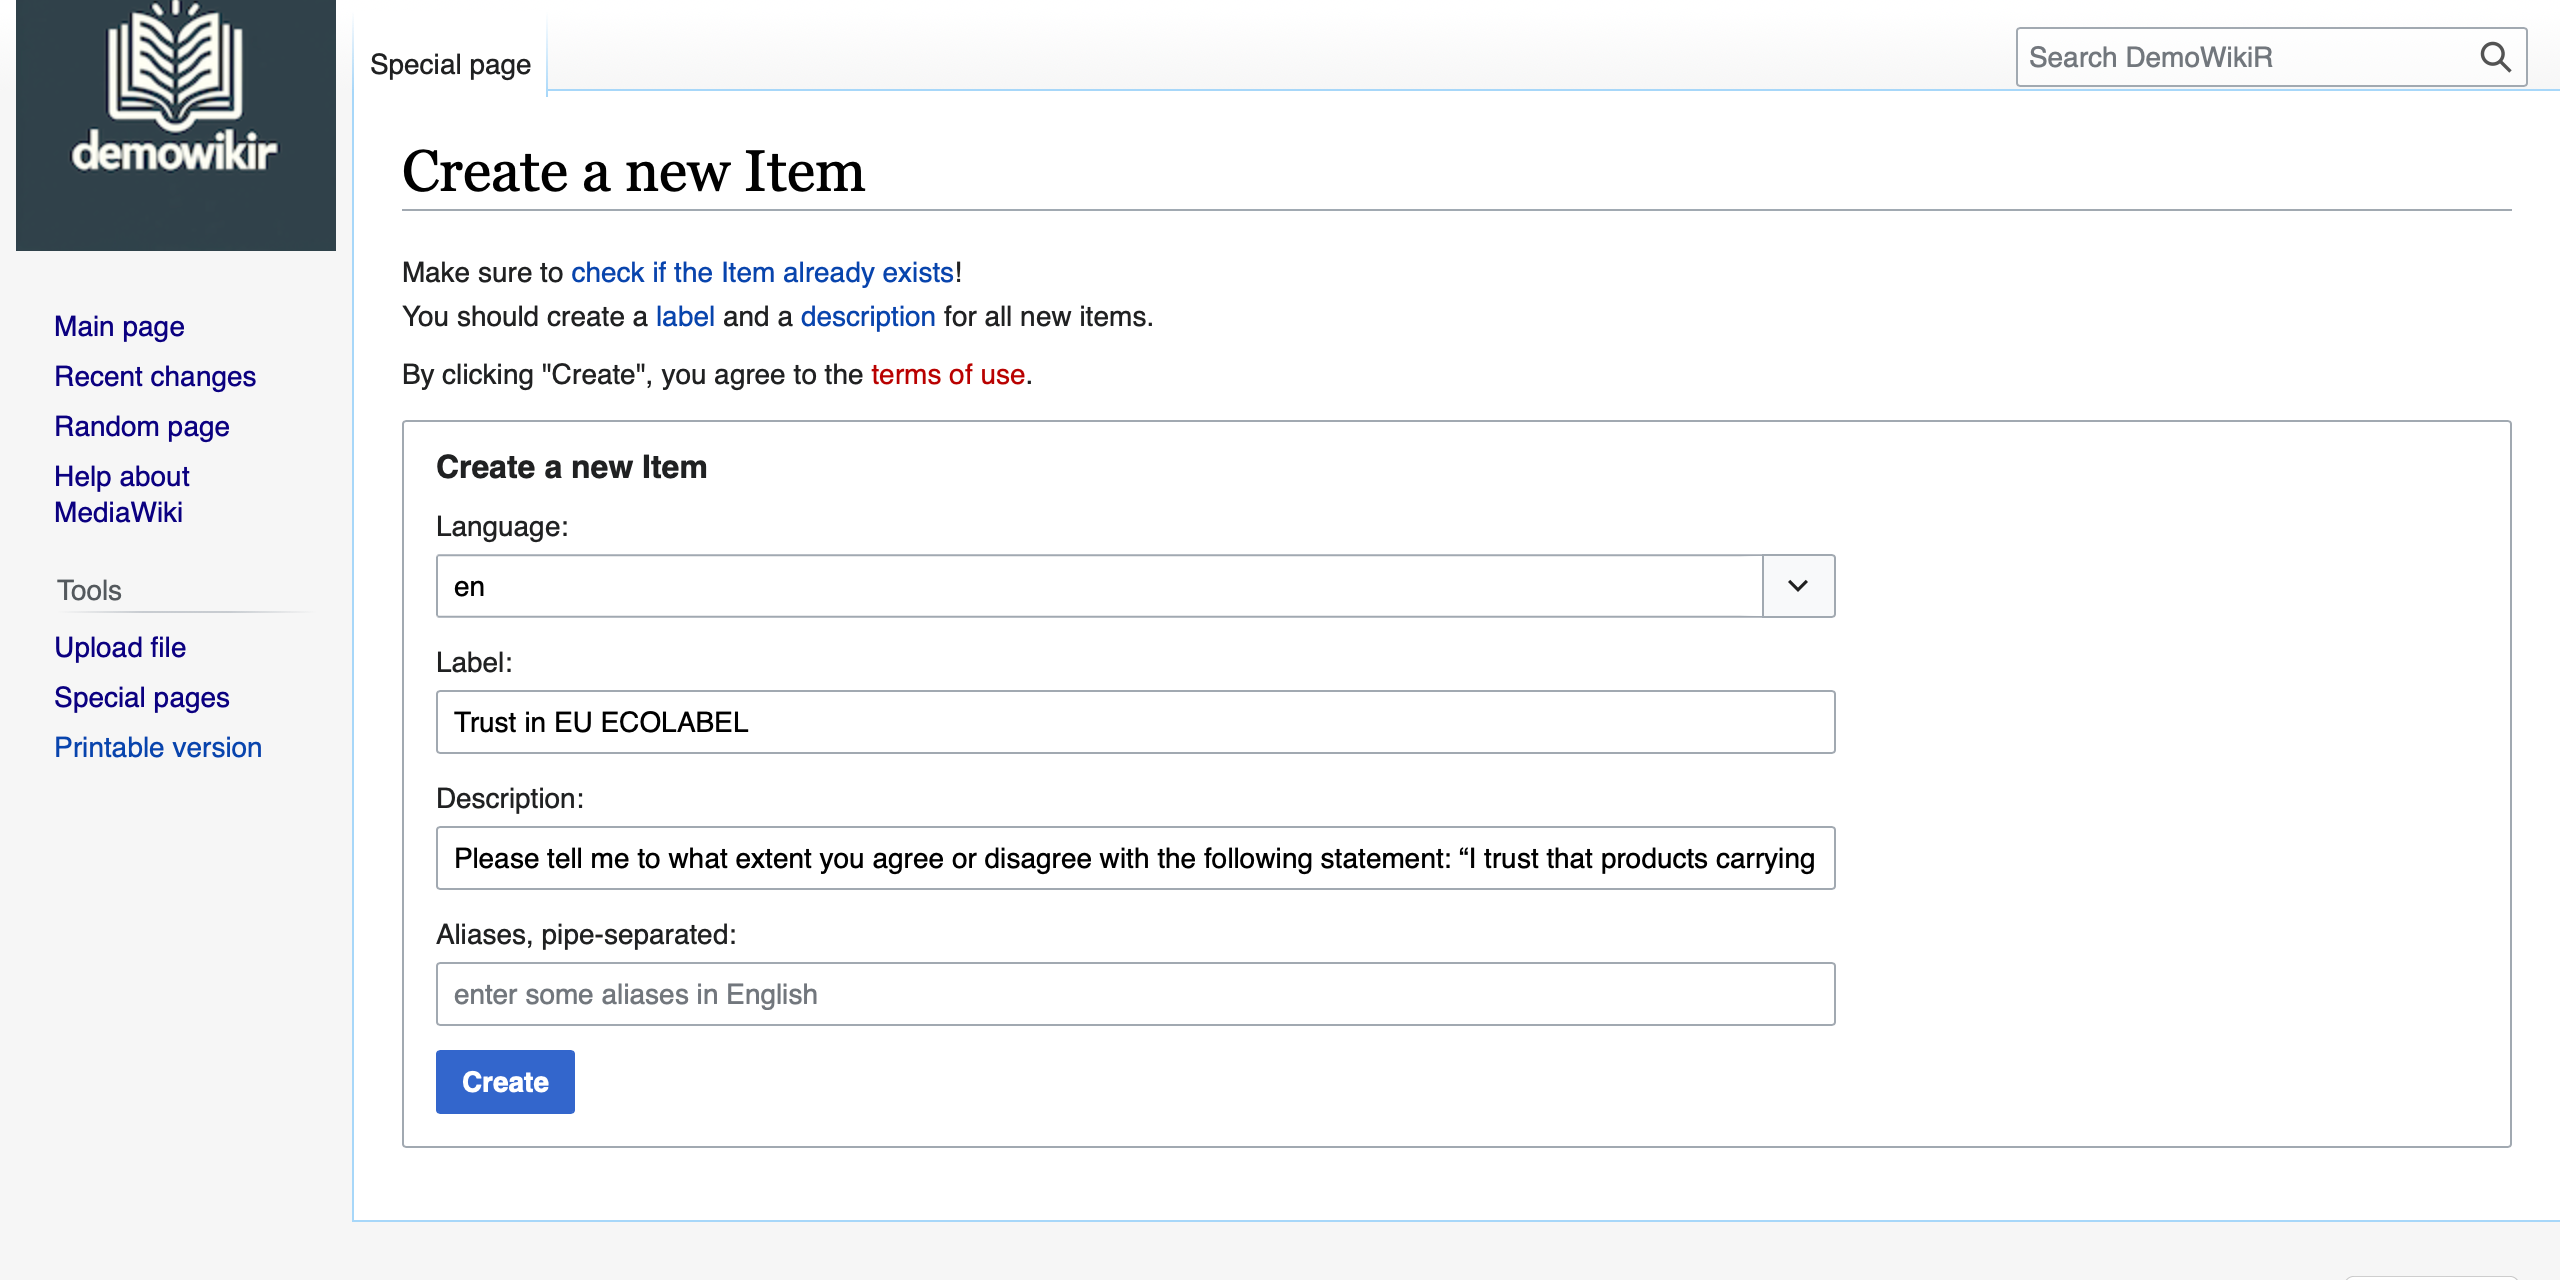
\includegraphics{png/question_to_wikibase/wikibase_createNewItem_2x1.png}
\end{center}

Click \texttt{Create}.

The question now is created on Wikibase.

\begin{center}
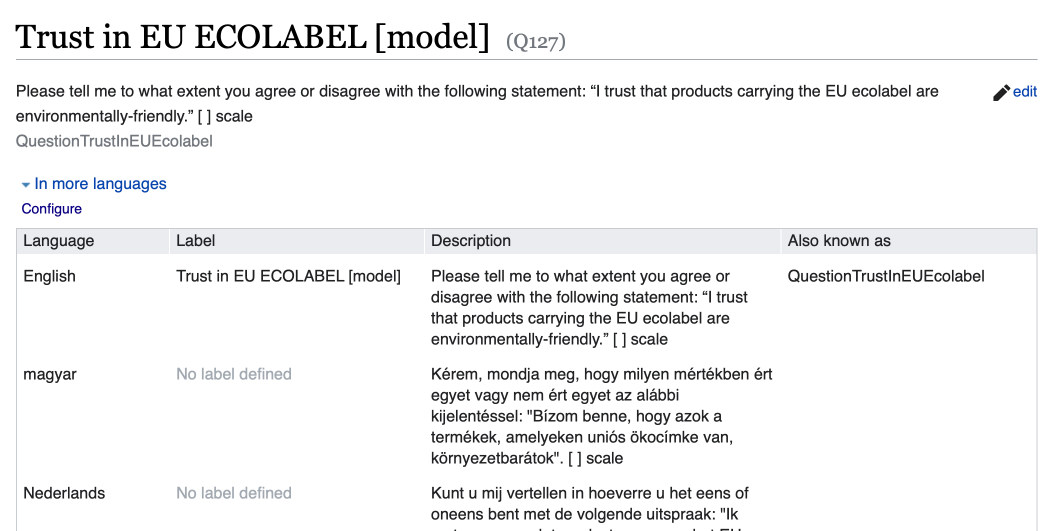
\includegraphics{png/question_to_wikibase/example_simple_question_2x1.png}
\end{center}

\begin{tcolorbox}[enhanced jigsaw, opacityback=0, bottomrule=.15mm, rightrule=.15mm, toptitle=1mm, breakable, colbacktitle=quarto-callout-note-color!10!white, colback=white, title=\textcolor{quarto-callout-note-color}{\faInfo}\hspace{0.5em}{Note}, leftrule=.75mm, toprule=.15mm, left=2mm, arc=.35mm, colframe=quarto-callout-note-color-frame, coltitle=black, titlerule=0mm, bottomtitle=1mm, opacitybacktitle=0.6]

Note: The system assigns a unique ID to every entry. In our example the
ID is
\href{https://reprexbase.eu/demowiki/index.php?title=Item:Q111}{Q111}.

\end{tcolorbox}

\subsubsection{Matrix Questions}\label{matrix-questions}

Matrix questions have:

\begin{itemize}
\item
  a model question
\item
  several question items
\item
  answer options
\end{itemize}

\begin{figure}[H]

{\centering 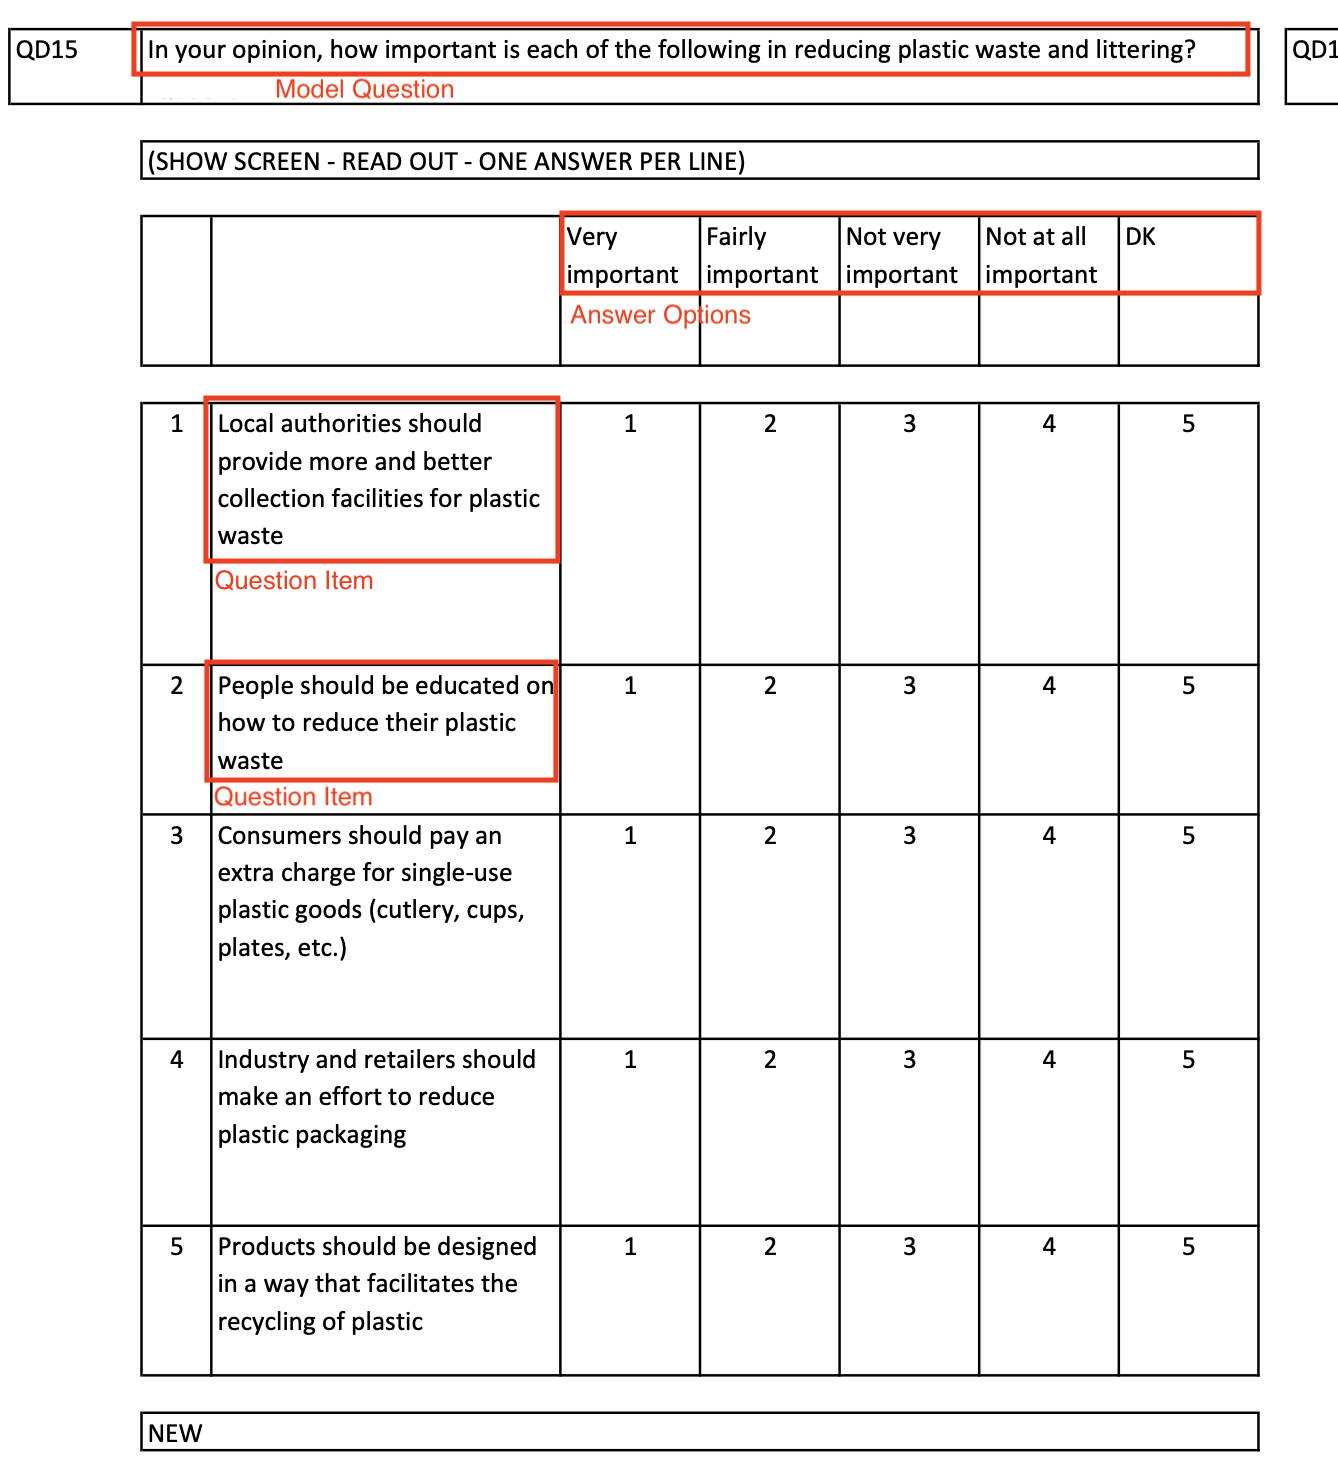
\includegraphics{png/question_to_wikibase/matrix_question.png}

}

\caption{This question is taken from the question block D (QD) from the
Eurobarometer 88.1 study.}

\end{figure}%

Following the functions ``Special Pages'' ▷ ``Create New Item'' you
should feed into Wibikbase separately the model question and the
questions items.

\begin{center}
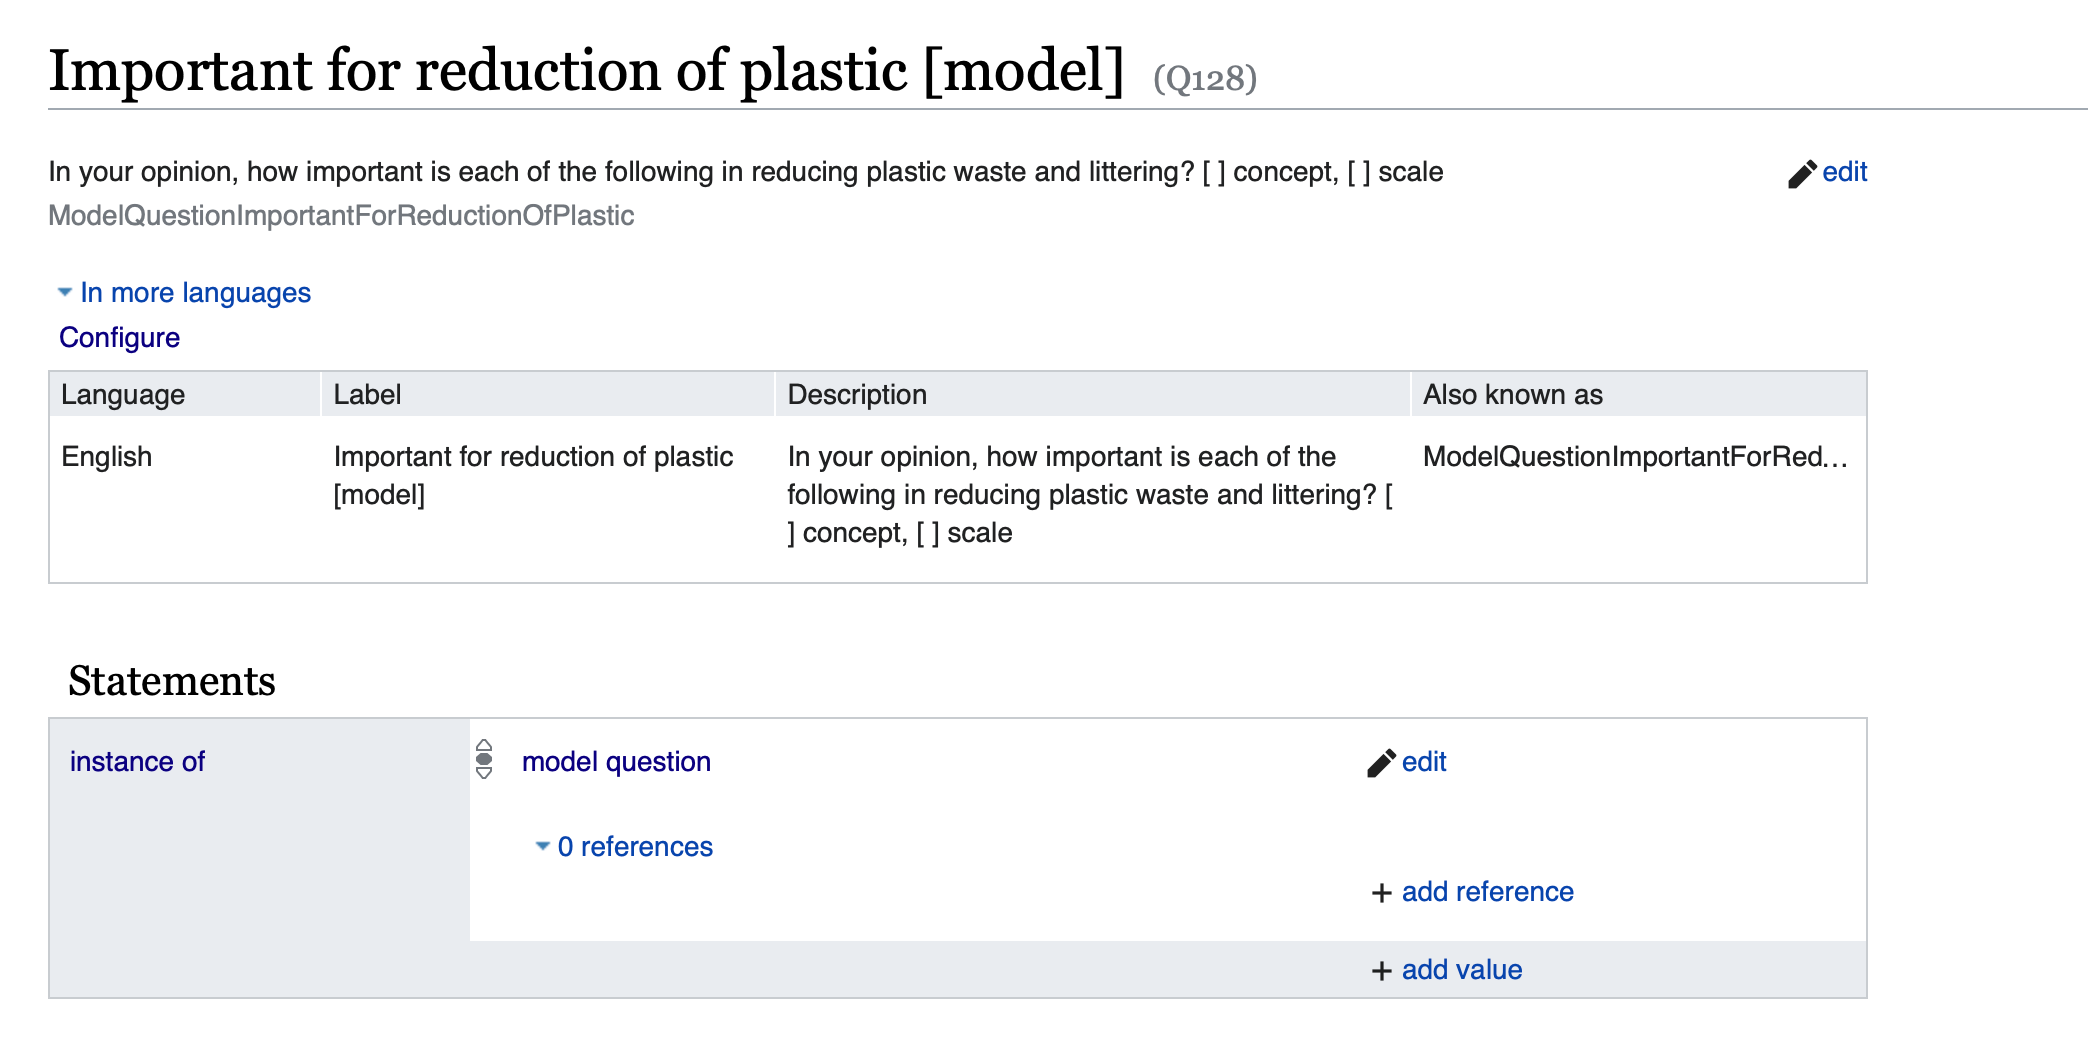
\includegraphics{png/question_to_wikibase/matrixQuestion_modelQuestion_2x1.png}
\end{center}

\href{https://reprexbase.eu/demowiki/index.php?title=Item:Q128}{Q128} is
the model question, which follows the structure:

\begin{itemize}
\item
  Language ▷ Choose the language (en)
\item
  Label - \emph{questionName + {[}model{]}} -
  \texttt{Important\ for\ reduction\ of\ plastic\ {[}model{]}}
\item
  questionText (description)

  \begin{itemize}
  \item
    \texttt{In\ your\ opinion,\ how\ important\ is\ each\ of\ the\ following\ in\ reducing\ plastic\ waste\ and\ littering?}
  \item
    \texttt{{[}\ {]}} \texttt{concept} - stands for the question items
  \item
    \texttt{{[}\ {]}} \texttt{scale} - stands for the answer options,
    which follow a scale
  \end{itemize}
\item
  Aliases - leave it empty
\end{itemize}

\begin{center}
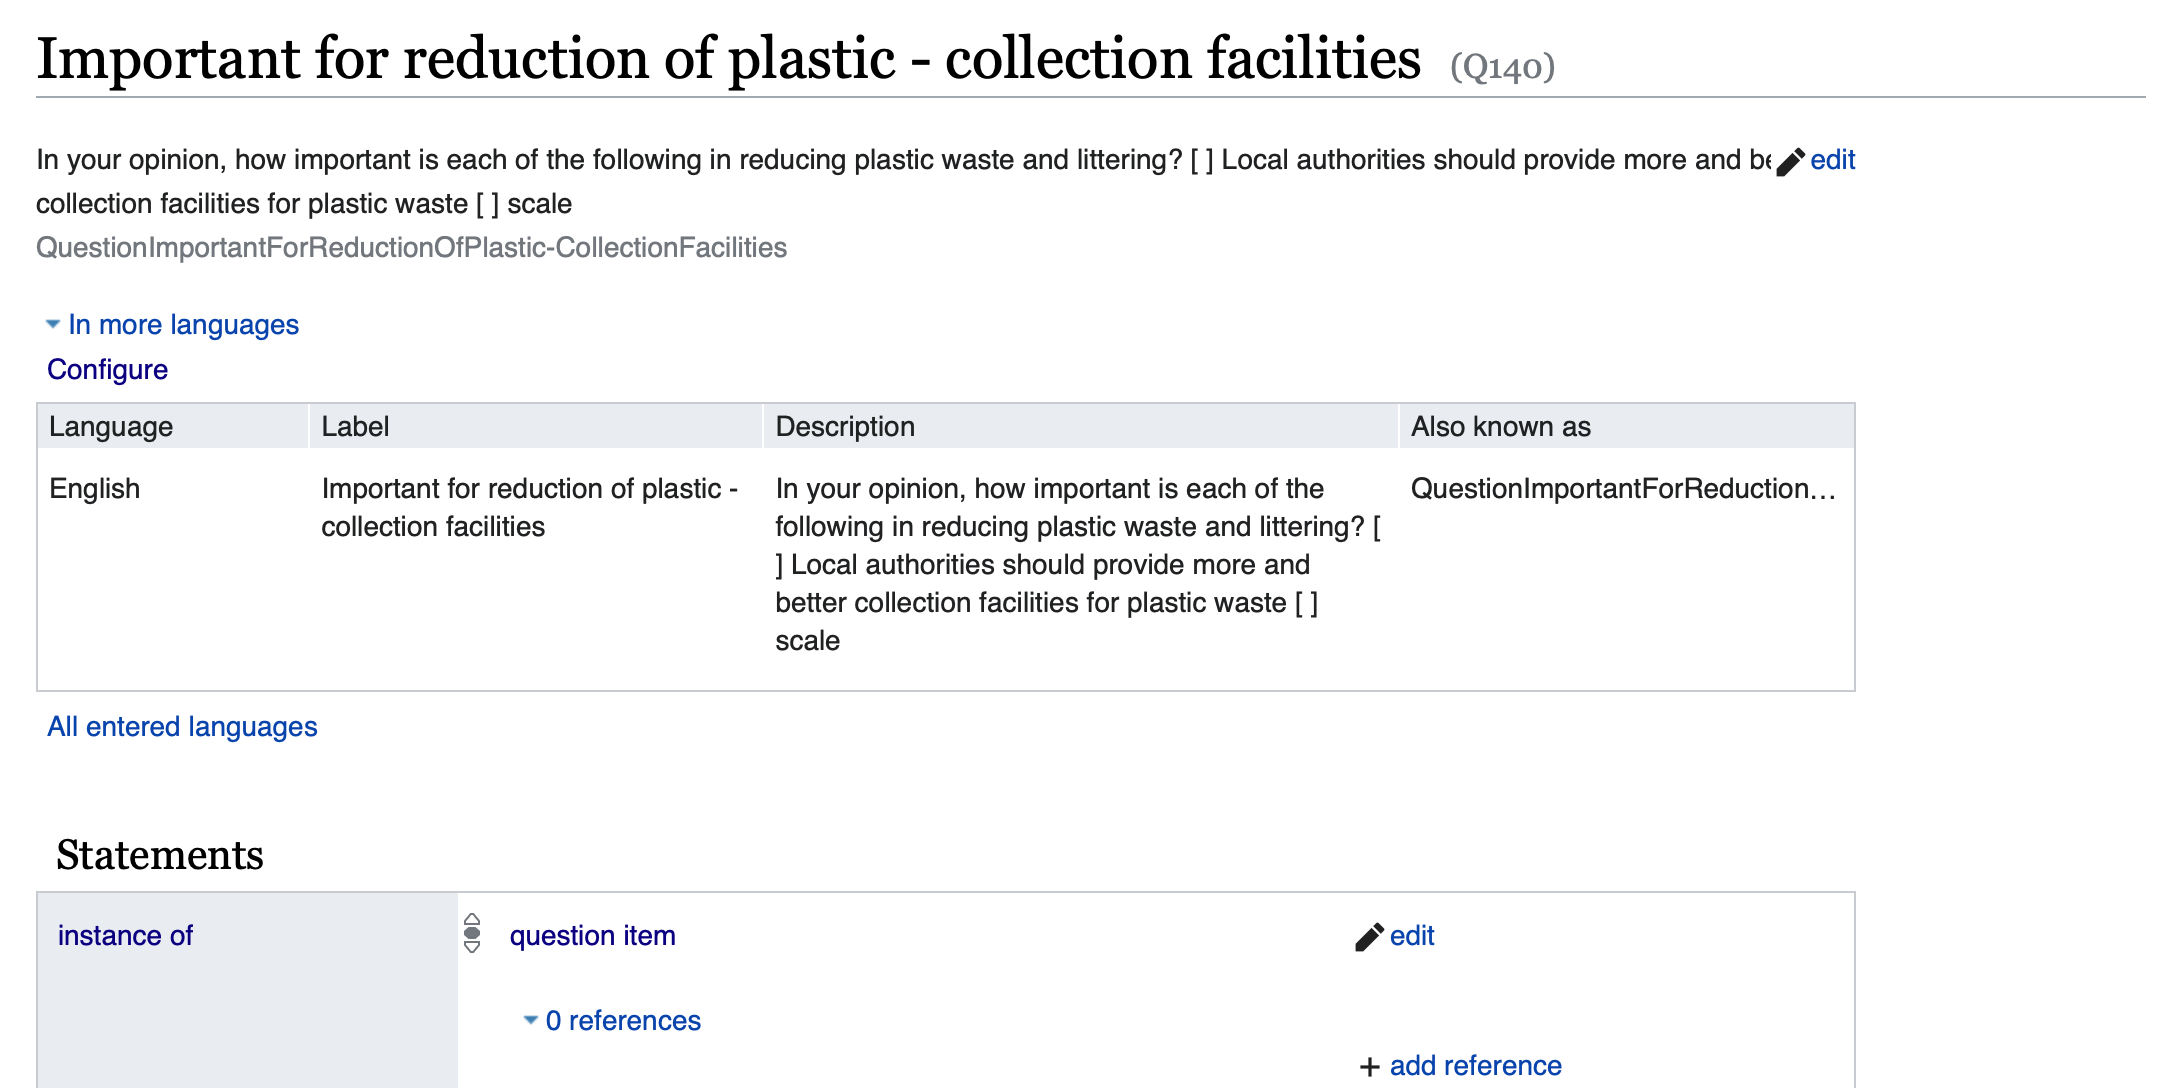
\includegraphics{png/question_to_wikibase/matrixQuestion_questionItem_2x1.png}
\end{center}

\href{https://reprexbase.eu/demowiki/index.php?title=Item:Q140}{Q140} is
a question item, which follows the structure:

\begin{itemize}
\tightlist
\item
  Language ▷ Choose the language (en)
\item
  label:
  \texttt{Important\ for\ reduction\ of\ plastic\ -\ collection\ facilities}
\item
  questionText (description)

  \begin{itemize}
  \tightlist
  \item
    model question -
    \texttt{In\ your\ opinion,\ how\ important\ is\ each\ of\ the\ following\ in\ reducing\ plastic\ waste\ and\ littering?}
  \item
    question item:
    \texttt{{[}\ {]}\ Local\ authorities\ should\ provide\ more\ and\ better\ collection\ facilities\ for\ plastic\ waste}
  \item
    \texttt{{[}\ {]}} \texttt{scale} - stands for the answer options,
    which follow a scale
  \end{itemize}
\item
  Aliases - leave it empty
\end{itemize}

\begin{tcolorbox}[enhanced jigsaw, opacityback=0, bottomrule=.15mm, rightrule=.15mm, toptitle=1mm, breakable, colbacktitle=quarto-callout-note-color!10!white, colback=white, title=\textcolor{quarto-callout-note-color}{\faInfo}\hspace{0.5em}{When creating a ``question item'', using statements, always connect the
``question item'' to the ``model question''}, leftrule=.75mm, toprule=.15mm, left=2mm, arc=.35mm, colframe=quarto-callout-note-color-frame, coltitle=black, titlerule=0mm, bottomtitle=1mm, opacitybacktitle=0.6]

\end{tcolorbox}

\begin{center}
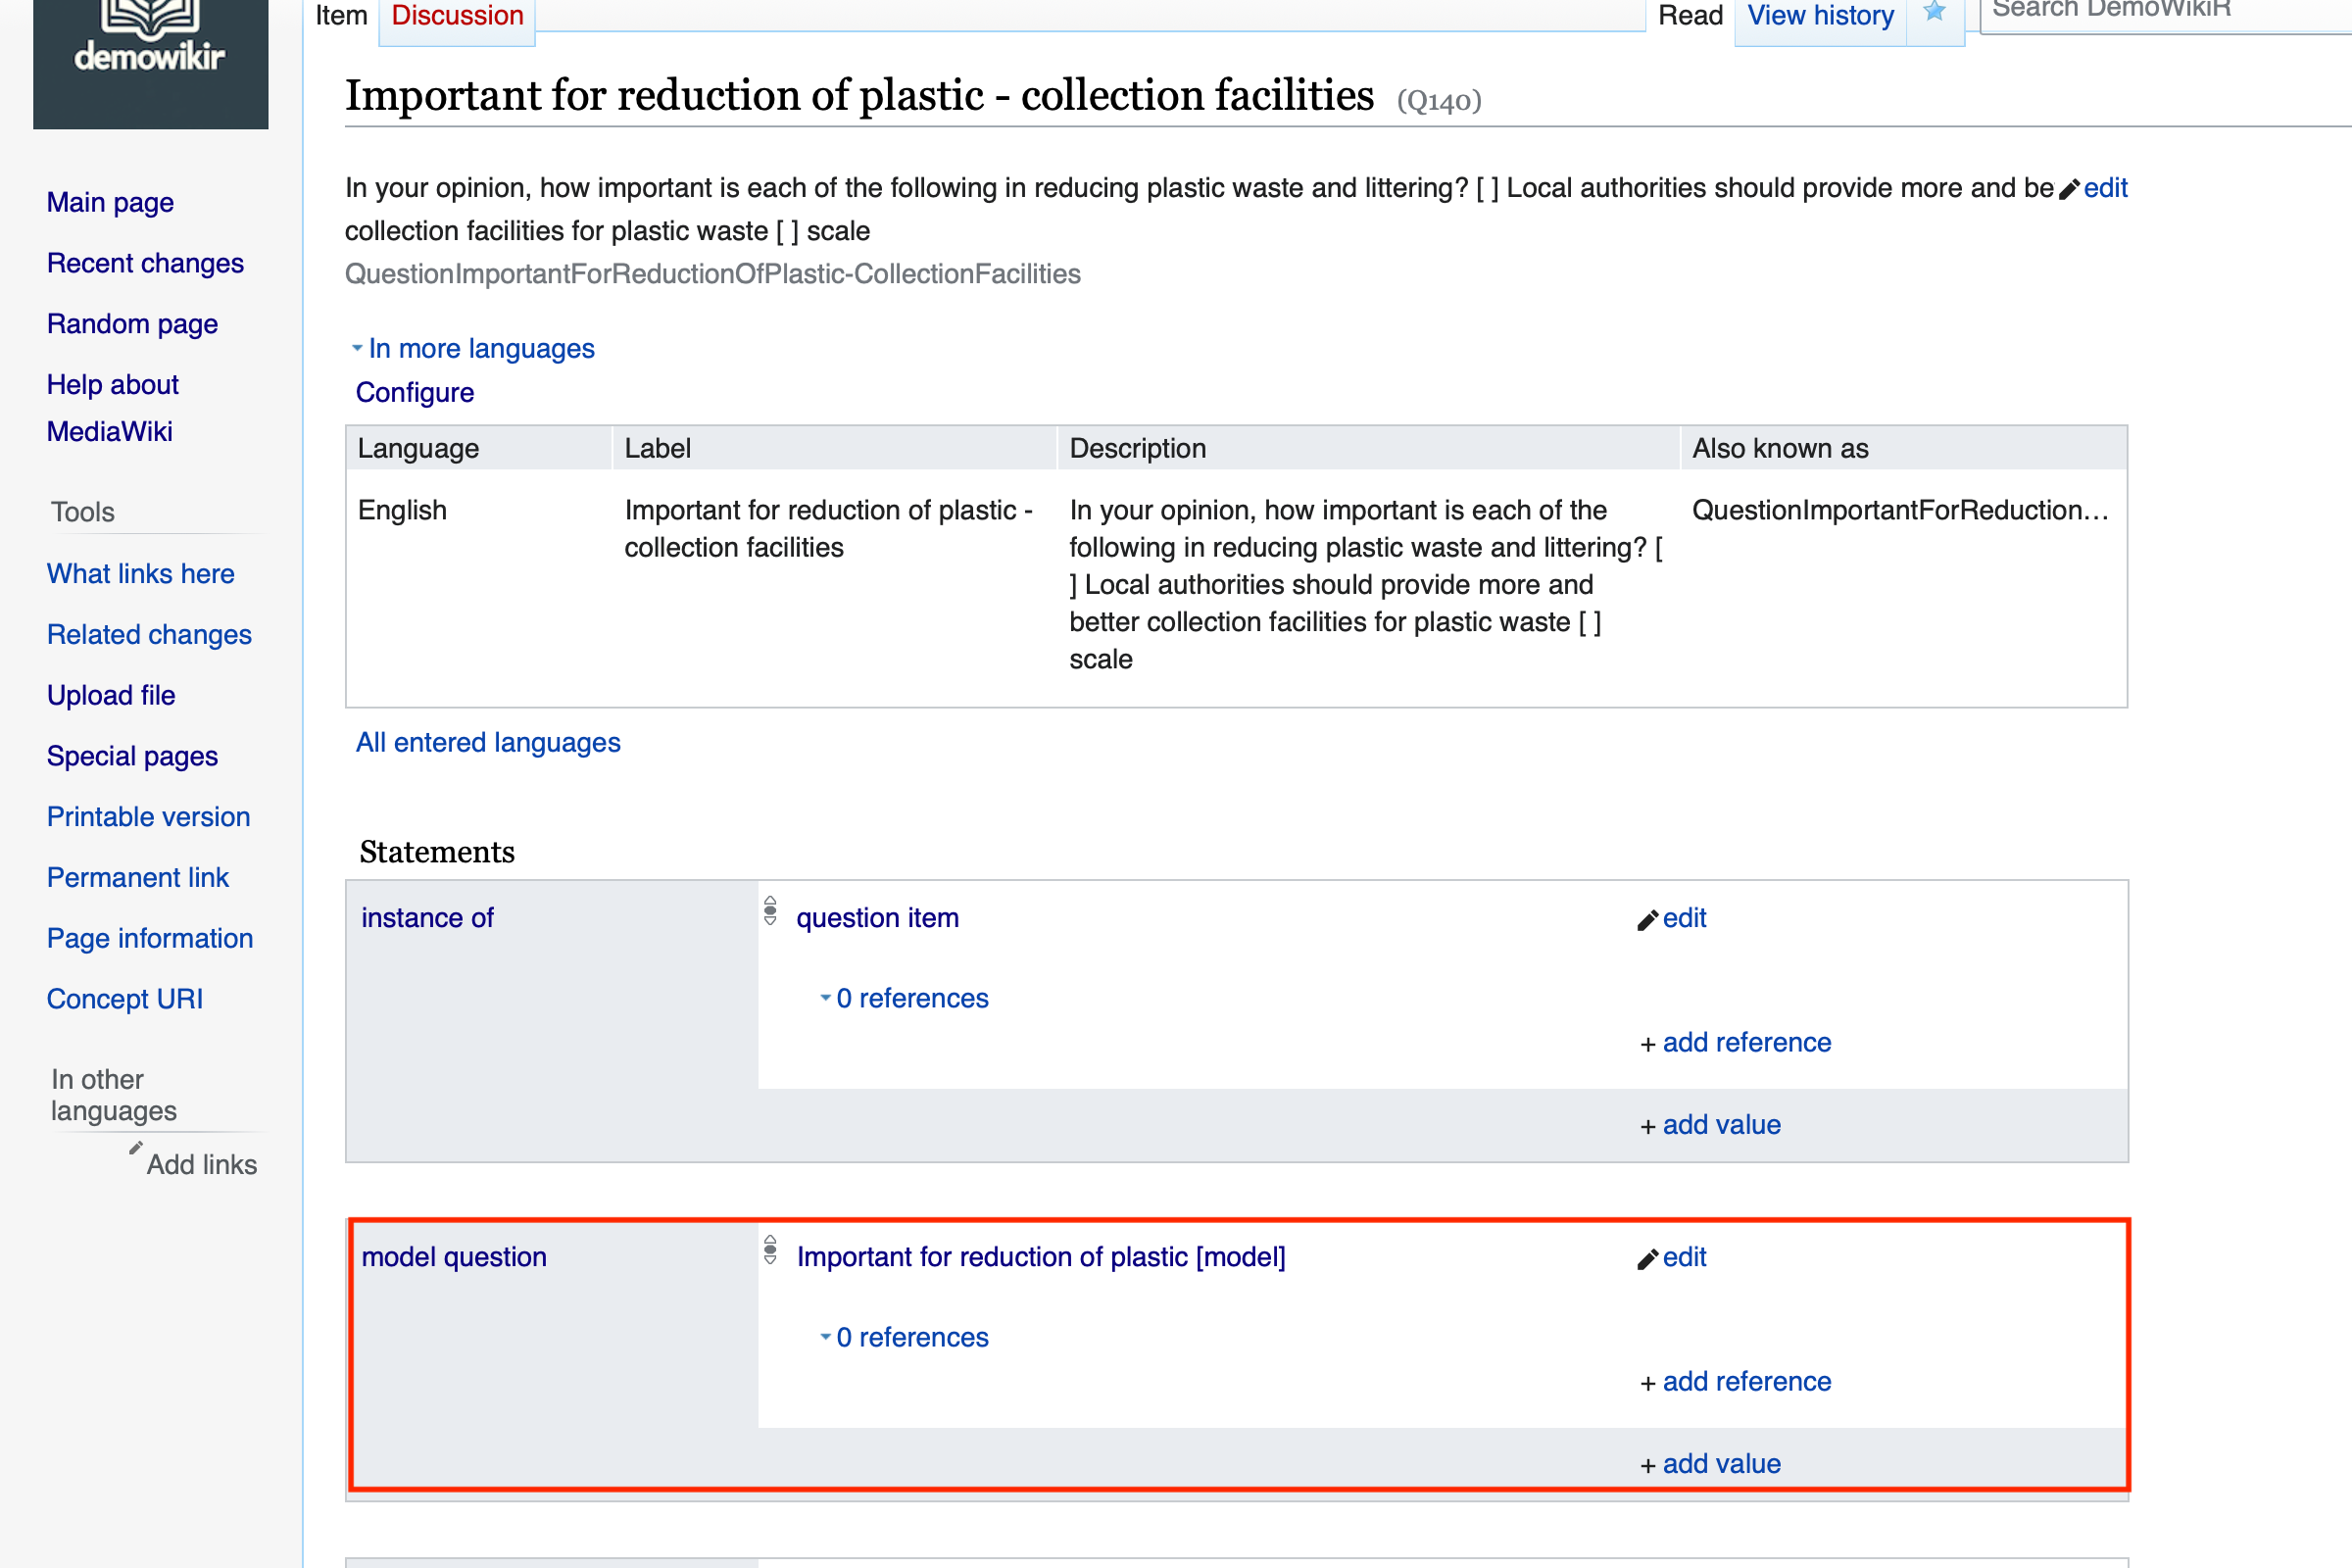
\includegraphics{png/question_to_wikibase/modelQuestion_questionItem_6x4.png}
\end{center}

\subsubsection{Multiple Choice
Questions}\label{multiple-choice-questions}

Multiple Choice questions have:

\begin{itemize}
\item
  a model question
\item
  several question items
\end{itemize}

\begin{figure}[H]

{\centering 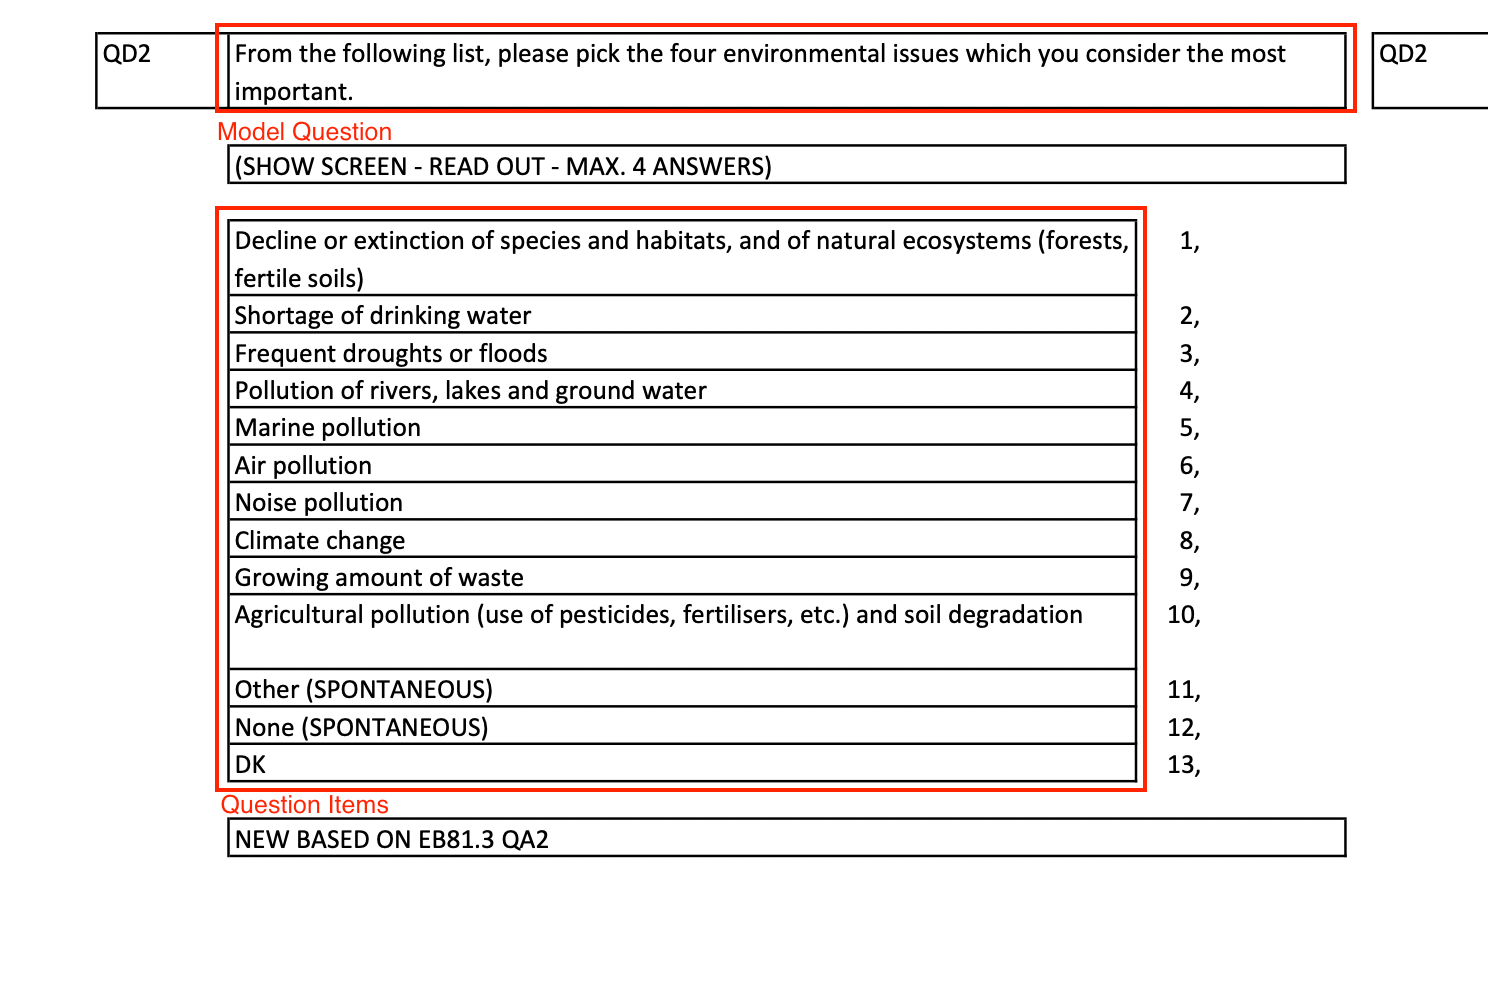
\includegraphics{png/question_to_wikibase/question_multipleChoice_6x4.png}

}

\caption{This question is taken from the question block D (QD) from the
Eurobarometer 88.1 study.}

\end{figure}%

Following the functions ``Special Pages'' ▷ ``Create New Item'' you
should feed into Wibikbase separately the model question and the
questions items.

\begin{center}
\includegraphics{png/question_to_wikibase/multipleChoiceQuestion_modelQuestion_2x1.png}
\end{center}

\href{https://reprexbase.eu/demowiki/index.php?title=Item:Q143}{Q143} is
the model question, which follows the structure:

\begin{itemize}
\item
  Language - Choose the language (en)
\item
  Label - \emph{questionName + {[}model{]}} -
  \texttt{Important\ environmental\ issue\textasciigrave{}\textasciigrave{}{[}model{]}}~
\item
  questionText (description)

  \begin{itemize}
  \item
    \texttt{From\ the\ following\ list,\ please\ pick\ the\ four\ environmental\ issues\ which\ you\ consider\ the\ most\ important.}
  \item
    \texttt{{[}\ {]}\ ranking} - stands for the question items
  \end{itemize}
\item
  Aliases: leave it empty
\end{itemize}

\begin{center}
\includegraphics{png/question_to_wikibase/multipleChoiceQuestion_questionItem_2x1.png}
\end{center}

\href{https://reprexbase.eu/demowiki/index.php?title=Item:Q144}{Q144} is
a question item, which follows the structure:

\begin{itemize}
\tightlist
\item
  Language ▷ Choose the language (en)
\item
  label:
  \texttt{Important\ for\ reduction\ of\ plastic\ -\ collection\ facilities}
\item
  questionText (description)

  \begin{itemize}
  \tightlist
  \item
    model question -
    \texttt{From\ the\ following\ list,\ please\ pick\ the\ four\ environmental\ issues\ which\ you\ consider\ the\ most\ important.}
  \item
    question item -
    \texttt{{[}\ {]}\ Decline\ or\ extinction\ of\ species\ and\ habitats,\ and\ of\ natural\ ecosystems\ (forests,\ fertile\ soils)}
  \end{itemize}
\item
  Aliases - leave it empty
\end{itemize}

\begin{tcolorbox}[enhanced jigsaw, opacityback=0, bottomrule=.15mm, rightrule=.15mm, toptitle=1mm, breakable, colbacktitle=quarto-callout-note-color!10!white, colback=white, title=\textcolor{quarto-callout-note-color}{\faInfo}\hspace{0.5em}{When creating a ``question item'', using statements, always connect the
``question item'' to the ``model question''}, leftrule=.75mm, toprule=.15mm, left=2mm, arc=.35mm, colframe=quarto-callout-note-color-frame, coltitle=black, titlerule=0mm, bottomtitle=1mm, opacitybacktitle=0.6]

\end{tcolorbox}

\section{Add Metadata Statements to your
Questions}\label{add-metadata-statements-to-your-questions}

Using Wikibase's ``statements'' feature you can link different type of
information to your questions.

You need to add further metadata statements to the question bank item.
Metadata is a statement about the data. We are adding standard, basic
statements in subject, predicate, and object (triplet) format to each
question bank item.

IN the following this guide explain how to add information about:

\begin{itemize}
\item
  questionnaire classes
\item
  \href{https://reprexbase.eu/demowiki/index.php?title=Property:P265}{variable
  representation (P265)}: a DDI-Lifecycle category for the creation of
  variables from the answer options, for example
\item
  \href{https://reprexbase.eu/demowiki/index.php?title=Property:P270}{study
  (DDI) P270}: the \emph{study} where you can find this (model) question
  (item). In DDI, a study represents the process by which a data set was
  generated or collected (in a survey). For example,
  \href{https://reprexbase.eu/demowiki/index.php?title=Item:Q139}{Eurobarometer
  88.1 (2017) Q139}
\item
  \href{https://reprexbase.eu/demowiki/index.php?title=Property:P267}{related
  survey concept (P267)}: a concept that a study (group), question
  (group) or question item aims to measure, for example
  \href{https://reprexbase.eu/demowiki/index.php?title=Item:Q131}{environmental
  protection (Q131)}.
\end{itemize}

\subsection{Questionnaire Classes}\label{questionnaire-classes}

Let's start by specifying the entry we created as
\texttt{model\ question} or \texttt{question\ item}.

Specify the entries created as \texttt{model\ question} or
\texttt{question\ item}.

\begin{itemize}
\item
  Select \texttt{+add\ statement}.
\item
  Using the
  \href{https://reprexbase.eu/demowiki/index.php?title=Property:P2}{instance
  of} property, which is defining the taxonomical class of the entered
  item (in this case, a question.)
\item
  In case of model questions, define them as \texttt{model\ question}.
\item
  In case of question item, define them as \texttt{question\ items}.
\end{itemize}

\begin{center}
\includegraphics{png/question_to_wikibase/instanceOf_modelQuestion_6x4.png}
\end{center}

\begin{tcolorbox}[enhanced jigsaw, opacityback=0, bottomrule=.15mm, rightrule=.15mm, toptitle=1mm, breakable, colbacktitle=quarto-callout-caution-color!10!white, colback=white, title=\textcolor{quarto-callout-caution-color}{\faFire}\hspace{0.5em}{In the case of questions items, always link them to the appropriate
model questions using the
\href{https://reprexbase.eu/demowiki/index.php?title=Property:P266}{model
question (P266)} property.}, leftrule=.75mm, toprule=.15mm, left=2mm, arc=.35mm, colframe=quarto-callout-caution-color-frame, coltitle=black, titlerule=0mm, bottomtitle=1mm, opacitybacktitle=0.6]

\end{tcolorbox}

\subsection{Variable Representation}\label{variable-representation}

When the questionnaire will be filled out in a raw dataset, each
response of a question(item) will be translated into a variable. We need
to define how we want to represent those answers in the resulting output
dataset. (See
\href{https://ddi-lifecycle-documentation.readthedocs.io/en/latest/TechnicalGuide/Value\%20Representation\%20and\%20Response\%20Domain.html}{DDI
3.3 (2020) documentation - Variable Value Representation and Question
Response Domain})

Using statements you can define the representation of the variables. You
can choose from the following categories:

\begin{itemize}
\item[$\boxtimes$]
  category representation base type: if the answers are categories (for
  example: \texttt{{[}\ {]}\ Female}, \texttt{{[}\ {]}\ Male},
  \texttt{{[}\ {]}\ Prefer\ not\ to\ say})
\item[$\boxtimes$]
  category representation base type with a \textbf{scale}: if the
  answers are categories and follow a scale (for example:
  \texttt{{[}{]}\ Very\ important},
  \texttt{{[}\ {]}\ Fairly\ important},
  \texttt{{[}\ {]}\ Not\ very\ important},
  \texttt{{[}\ {]}\ Not\ at\ all\ important}. )
\item[$\boxtimes$]
  ranking representation base type: the respondant must rank the answer
  options, like 1st, 2nd, 3rd, etc.
\item[$\boxtimes$]
  numeric variable representation base type: the answer should be a
  number, for example, the age of the respondant as an integer number or
  a postal code in a country where postal codes contain only numeric
  digits, f.e., \texttt{1051}.
\item[$\boxtimes$]
  textual variable representation base type: the answer should be some
  text, for example, and open answer, or a geographical location typed
  as a simple text, for example, \texttt{Bratislava}.
\end{itemize}

\begin{center}
\includegraphics{png/question_to_wikibase/VariableRepresentation_6x4.png}
\end{center}

\subsection{Define the source study}\label{define-the-source-study}

\begin{tcolorbox}[enhanced jigsaw, opacityback=0, bottomrule=.15mm, rightrule=.15mm, toptitle=1mm, breakable, colbacktitle=quarto-callout-tip-color!10!white, colback=white, title=\textcolor{quarto-callout-tip-color}{\faLightbulb}\hspace{0.5em}{Tip}, leftrule=.75mm, toprule=.15mm, left=2mm, arc=.35mm, colframe=quarto-callout-tip-color-frame, coltitle=black, titlerule=0mm, bottomtitle=1mm, opacitybacktitle=0.6]

For further details, please check the
\href{https://rdf-vocabulary.ddialliance.org/discovery.html\#study}{disco:Study}
class.

\end{tcolorbox}

With the
\href{https://reprexbase.eu/demowiki/index.php?title=Property:P270}{study
(DDI) P270} property you must link as a statement the \emph{study} where
you found the (model) question (item).

\begin{center}
\includegraphics{png/question_to_wikibase/statement_study_2x1.png}
\end{center}

An example for a study:
\href{https://reprexbase.eu/demowiki/index.php?title=Item:Q139}{Eurobarometer
88.1 (2017) Q139}

\begin{tcolorbox}[enhanced jigsaw, opacityback=0, bottomrule=.15mm, rightrule=.15mm, toptitle=1mm, breakable, colbacktitle=quarto-callout-note-color!10!white, colback=white, title=\textcolor{quarto-callout-note-color}{\faInfo}\hspace{0.5em}{Note}, leftrule=.75mm, toprule=.15mm, left=2mm, arc=.35mm, colframe=quarto-callout-note-color-frame, coltitle=black, titlerule=0mm, bottomtitle=1mm, opacitybacktitle=0.6]

Note: If the study is not yet in Wikibase, you can create an entry for
it using the \texttt{Create\ a\ New\ Item} function.

\end{tcolorbox}

\subsection{Add related concept}\label{add-related-concept}

With the
\href{https://reprexbase.eu/demowiki/index.php?title=Property:P267}{related
survey concept (P267)} property you can link concepts, that a study
(group), question (group) or question item aims to measure, for example
\href{https://reprexbase.eu/demowiki/index.php?title=Item:Q131}{environmental
protection (Q131)}.

\begin{center}
\includegraphics{png/question_to_wikibase/statement_relatedSurveyConcept_2x1.png}
\end{center}

Where are the related concepts coming from?

1. The best case is that you use a widely accepted conceptualisation
(ontology item) of your domain. For example, we took the
\href{https://reprexbase.eu/demowiki/index.php?title=Item:Q138}{study
(Q149)} concept from the DDI-Discovery (disco) ontology. You can connect
statements of equivalence to a well-defined ontology via
\href{https://reprexbase.eu/demowiki/index.php?title=Property:P69}{equivalent
class (P69)}. In other words, our Q149 entity is equivalent to DDI's
\texttt{Study}.

2. If there are no accepted ontologies or you are uncertain, it is a
very good practice to use a concept definition from Wikidata. Even in
the case of an ontological definition, adding the Wikidata QID is a
great idea because Wikidata connects equivalent definitions across
various domains' ontologies. You can make a statement about an
equivalent Wikidata URI (for an item) by
\href{https://reprexbase.eu/demowiki/index.php?title=Property:P73}{Wikibase
URI (P73)}. See, for example
\href{https://reprexbase.eu/demowiki/index.php?title=Item:Q148}{plastic
(Q148)},
\href{https://reprexbase.eu/demowiki/index.php?title=Property:P73}{Wikibase
URI (P73)}, \url{https://www.wikidata.org/wiki/Q11474}, meaning that our
\texttt{plastic} definition is equivalent to the Wikidata definition of
\texttt{plastic}.

3. You can create your definition if you are still looking for a
suitable definition in an accepted ontology or on Wikidata. For this,
you should create a definition in Wikibase (as a new item.) See, for
example,
\href{https://reprexbase.eu/demowiki/index.php?title=Item:Q126}{model
question (Q126)}, which is our own proprietary definition until we find
a more consensual one.

\section{Add the questionText
translations}\label{add-the-questiontext-translations}

On Wikibase you can add different language versions to the same
question.

To do so, go to ``Special Pages''

\begin{center}
\includegraphics{png/question_to_wikibase/wikidata_specialPages_2x1.png}
\end{center}

Scroll down and select: ``Set Item/Property Description''

\begin{center}
\includegraphics{png/question_to_wikibase/SpecialPages_Set_ItemProperty_Description_2x1.png}
\end{center}

Fill the form:

\begin{itemize}
\item
  ID - The QiD of the question
\item
  Language code - the new language you want to input the question
\item
  Description - The question itself in the new language
\end{itemize}

\begin{center}
\includegraphics{png/question_to_wikibase/Set_IetmProperty_Description_2x1.png}
\end{center}
Select ``Set Description''.

The entry is now updated with another language.

\chapter{Variables in Music Databases}\label{sec-musicapi}

We use two information models:

\begin{itemize}
\tightlist
\item
  SDMX for statistical concepts
\item
  DDI for the documentation of microdata
\end{itemize}

When repeatedly querying a music API, such as the Spotify API, we carry
out an automated survey in which the respondent is not a human but a
machine. Sending the same query to a well-designed API will yield a
comparable answer to our question sent to the same API yesterday or
tomorrow.

There are still many similarities with survey harmonisation: you would
usually like to combine the data from the API with other data sources,
in which case you still have to harmonise the concepts, the labelling,
the translations, and the coding of your responses (processed in a
dataset into variables.)

The previous Appendix introduces the key concepts and practices of
survey harmonisation. When working with APIs, you do not need to
harmonise question texts in human languages, because you harmonise them
in a marchine-readable query language (for example, in SQL or SPARQL.)
The rest of the data harmonisation workflow is the same.

\section{String versus item}\label{string-versus-item}

\begin{itemize}
\tightlist
\item
  \href{https://reprexbase.eu/demowiki/index.php?title=Item:Q79}{Slovakia
  (Q79)} is a well-defined node in our Wikibase graph.
\item
  \texttt{Slovakia} as a string is not well-defined; it can only be
  understood if we add \texttt{"Slovakia"@en} a reference to the natural
  language of the string.
\end{itemize}

Whenever possible, we want to refer to well-defined nodes in the
knowledge graph. For example, our entry
\href{https://reprexbase.eu/demowiki/index.php?title=Item:Q79}{Slovakia
(Q79)} states that it is equivalent with
\href{https://www.wikidata.org/wiki/Q214}{Slovakia (Q214) on Wikidata},
and Wikidata connects plenty of metadata to this concept: the
geographical boundaries, the fact that it is an independent state since
1993, it predecessors, capital, etc.

Our aim is to have a rich and standardised description to each variable,
and as much as possible, to very constant (or attribute.) \emph{Katarína
Kubošiová} is a Slovak singer-songwriter, also known as \emph{Katarzia}.
To avoid any ambigouity with other people potentially called
\emph{Katarína Kubošiová} or \emph{Katarzia}, we would like to refer to
her with a globally unique identifier. Her ISNI identifier (ISNI: ) is
\href{https://isni.org/isni/0000000467220673}{isni: 0000000467220673},
which identifies her with global clarity.

The metadata enrichment is possible to make data points into nodes. For
example, if we conceptualise \texttt{Slovakia} into a node, than we can
connect to this node sound recordings (regardless if they have a Slovak
or English-language title) if they were registered with the Slovak
national ISRC registrant's \texttt{SK} prefix. We can connect
\texttt{Katarína\ Kubošiová}, \texttt{Katarzia}, \texttt{SK},
\texttt{Slovakia} in a graph to the concept of \emph{Slovakia} with less
or more clarity; in this case, for example, defining that a sound
recording was registered in Slovakia, or the artist known as
\emph{Katarzia} was born in Slovakia or sung in the Slovak language.

\subsection{1. Access Wikibase}\label{access-wikibase}

Login in with you account to Wikibase.

\subsection{2. Create a New Item}\label{create-a-new-item}

Go to \texttt{Special\ Pages}

\begin{center}
\includegraphics{png/question_to_wikibase/wikidata_specialPages_2x1.png}
\end{center}

Scroll down and select: \texttt{Create\ a\ New\ Item}

\begin{center}
\includegraphics{png/question_to_wikibase/wikibase_addNewItem_2x1.png}
\end{center}

Fill the form with the item's data:

\begin{itemize}
\item
  Language - Choose the language (en)
\item
  Label - Give a short name for the node, for example, \emph{Katarína
  Kubošiová}
\item
  Description - Enter the item description, for example
  \emph{Singer-songwriter born in the Slovak Republic}
\item
  Aliases - you can add \emph{Katarzia} or any other known names here.
\end{itemize}

\begin{center}
\includegraphics{png/question_to_wikibase/wikibase_createNewItem_2x1.png}
\end{center}

Click \texttt{Create}.

The item now is created on Wikibase. For each concept that you want to
use in your research, its documentation should be present. For key
persons, names, musical works, it is also advisable to have an item
defined.

\begin{center}
\includegraphics{png/question_to_wikibase/example_question_2x1.png}
\end{center}

\begin{tcolorbox}[enhanced jigsaw, opacityback=0, bottomrule=.15mm, rightrule=.15mm, toptitle=1mm, breakable, colbacktitle=quarto-callout-note-color!10!white, colback=white, title=\textcolor{quarto-callout-note-color}{\faInfo}\hspace{0.5em}{Note}, leftrule=.75mm, toprule=.15mm, left=2mm, arc=.35mm, colframe=quarto-callout-note-color-frame, coltitle=black, titlerule=0mm, bottomtitle=1mm, opacitybacktitle=0.6]

Note: The system assigns a unique ID to every entry. For example, in our
system, the ID of \emph{Ján Levoslav Bella} (Slovak conductor, composer
and educator), aslo known under the alias with no Slovak special
characters as \emph{Jan Levoslav Bella} is
\href{https://reprexbase.eu/demowiki/index.php?title=Item:Q93}{Q93}.
With Q93 you cannot make the mistake of confusing the fact that
\emph{Ján Levoslav Bella} is the same person as \emph{Jan Levoslav
Bella}.

\end{tcolorbox}

\subsection{3. Add Metadata Statements}\label{add-metadata-statements}

You need to add further metadata statements to the question bank item.
Metadata is a statement about the data. We are adding standard, basic
statements in subject, predicate, and object (triplet) format to each
question bank item.

\subsubsection{Variable Representation}\label{variable-representation-1}

DDI has standard variable representation definitions. When a
questionnaire will be filled out in a raw dataset, or data will be
systematically queried from and API, each response will be translated
into a variable. We need to define how we want to represent those
answers in the resulting output dataset. (See
\href{https://ddi-lifecycle-documentation.readthedocs.io/en/latest/TechnicalGuide/Value\%20Representation\%20and\%20Response\%20Domain.html}{DDI
3.3 (2020) documentation - Variable Value Representation and Question
Response Domain})

Using statements you can define the representation of the variables. You
can choose from the following categories:

\begin{itemize}
\item[$\boxtimes$]
  category representation base type: if the answers are categories (for
  example: \texttt{{[}\ {]}\ Female}, \texttt{{[}\ {]}\ Male},
  \texttt{{[}\ {]}\ Prefer\ not\ to\ say})
\item[$\boxtimes$]
  category representation base type with a \textbf{scale}: if the
  answers are categories and follow a scale (for example:
  \texttt{{[}{]}\ Very\ important},
  \texttt{{[}\ {]}\ Fairly\ important},
  \texttt{{[}\ {]}\ Not\ very\ important},
  \texttt{{[}\ {]}\ Not\ at\ all\ important}. )
\item[$\boxtimes$]
  ranking representation base type: the respondant must rank the answer
  options, like 1st, 2nd, 3rd, etc.
\item[$\boxtimes$]
  numeric variable representation base type: the answer should be a
  number, for example, the age of the respondant as an integer number or
  a postal code in a country where postal codes contain only numeric
  digits, f.e., \texttt{1051}.
\item[$\boxtimes$]
  textual variable representation base type: the answer should be some
  text, for example, and open answer, or a geographical location typed
  as a simple text, for example, \texttt{Bratislava}.
\end{itemize}

\begin{center}
\includegraphics{png/question_to_wikibase/VariableRepresentation_6x4.png}
\end{center}

\subsubsection{Define the source study}\label{define-the-source-study-1}

\begin{tcolorbox}[enhanced jigsaw, opacityback=0, bottomrule=.15mm, rightrule=.15mm, toptitle=1mm, breakable, colbacktitle=quarto-callout-tip-color!10!white, colback=white, title=\textcolor{quarto-callout-tip-color}{\faLightbulb}\hspace{0.5em}{Tip}, leftrule=.75mm, toprule=.15mm, left=2mm, arc=.35mm, colframe=quarto-callout-tip-color-frame, coltitle=black, titlerule=0mm, bottomtitle=1mm, opacitybacktitle=0.6]

For further details, please check the
\href{https://rdf-vocabulary.ddialliance.org/discovery.html\#study}{disco:Study}
class.

\end{tcolorbox}

With the
\href{https://reprexbase.eu/demowiki/index.php?title=Property:P270}{study
(DDI) P270} property you must link as a statement the \emph{study} where
you found the concept definition. If it was a formal ontology, or
Wikibase, use different properties (see below).

\begin{center}
\includegraphics{png/question_to_wikibase/statement_study_2x1.png}
\end{center}

An example for a study:
\href{https://reprexbase.eu/demowiki/index.php?title=Item:Q139}{Eurobarometer
88.1 (2017) Q139}

\begin{tcolorbox}[enhanced jigsaw, opacityback=0, bottomrule=.15mm, rightrule=.15mm, toptitle=1mm, breakable, colbacktitle=quarto-callout-note-color!10!white, colback=white, title=\textcolor{quarto-callout-note-color}{\faInfo}\hspace{0.5em}{Note}, leftrule=.75mm, toprule=.15mm, left=2mm, arc=.35mm, colframe=quarto-callout-note-color-frame, coltitle=black, titlerule=0mm, bottomtitle=1mm, opacitybacktitle=0.6]

Note: If the study is not yet in Wikibase, you can create an entry for
it using the \texttt{Create\ a\ New\ Item} function.

\end{tcolorbox}

\subsubsection{Add related concept}\label{add-related-concept-1}

Where are the related concepts coming from?

\begin{enumerate}
\def\labelenumi{\arabic{enumi}.}
\item
  The best case is that you use a widely accepted conceptualisation
  (ontology item) of your domain. For example, we took the
  \href{https://reprexbase.eu/demowiki/index.php?title=Item:Q132}{duration
  (Q132)} concept from the Music Ontology. You can connect statements of
  equivalence to a well-defined ontology via
  \href{https://reprexbase.eu/demowiki/index.php?title=Property:P69}{equivalent
  class (P69)}. In other words, our Q149 entity is equivalent to Music
  Ontology's \texttt{duration} (in short: \texttt{mo:duration}.)
\item
  If there are no accepted ontologies or you are uncertain, it is a very
  good practice to use a concept definition from Wikidata. Even in the
  case of an ontological definition, adding the Wikidata QID is a great
  idea because Wikidata connects equivalent definitions across various
  domains' ontologies. You can make a statement about an equivalent
  Wikidata URI (for an item) by
  \href{https://reprexbase.eu/demowiki/index.php?title=Property:P73}{Wikibase
  URI (P73)}. See, for example
  \href{https://reprexbase.eu/demowiki/index.php?title=Item:Q132}{duration
  (Q132)},
  \href{https://reprexbase.eu/demowiki/index.php?title=Property:P73}{Wikibase
  URI (P73)},
  \href{https://www.wikidahttps://www.wikidata.org/wiki/Q16038819}{https://www.wikidata.org/wiki/Q16038819},
  meaning that our \texttt{plastic} definition is equivalent to the
  Wikidata definition of \texttt{plastic} (which has a QID of
  \texttt{Q16038819} on Wikidata, and it received the QID of
  \texttt{Q132} on our Wikibase instance.)
\item
  You can create your definition if you are still looking for a suitable
  definition in an accepted ontology or on Wikidata. For this, you
  should create a definition in Wikibase (as a new item.) See, for
  example,
  \href{https://reprexbase.eu/demowiki/index.php?title=Item:Q126}{model
  question (Q126)}, which is our own proprietary definition until we
  find a more consensual one.
\end{enumerate}

\subsection{Add national langugage translations to your
concept}\label{add-national-langugage-translations-to-your-concept}

On Wikibase you can add different language versions to the same
question.

To do so, go to \texttt{Special\ Pages}

\begin{center}
\includegraphics{png/question_to_wikibase/wikidata_specialPages_2x1.png}
\end{center}

Scroll down and select: \texttt{Set\ Item/Property\ Description}

\begin{center}
\includegraphics{png/question_to_wikibase/SpecialPages_Set_ItemProperty_Description_2x1.png}
\end{center}

Fill the form:

\begin{itemize}
\item
  ID - The QiD of the question (for example, if you want to add a Dutch
  description to \emph{Ján Levoslav Bella}, i.e., Slovak conductor,
  composer and educator, you must reference
  \href{https://reprexbase.eu/demowiki/index.php?title=Item:Q93}{Q93}.
\item
  Language code - the new language you want to input the question, in
  this case, \texttt{nl}.
\item
  Description - Write a short definition (up to 250 characters) in the
  new language.
\end{itemize}

\begin{center}
\includegraphics{png/question_to_wikibase/Set_IetmProperty_Description_2x1.png}
\end{center}
Select ``Set Description''.

The entry is now updated with another language label or description.




\end{document}
